\documentclass[a4paper,7pt]{book}

\usepackage[a5paper,bindingoffset=10mm,left=15mm,right=15mm,top=15mm,bottom=15mm,footskip=10mm]{geometry}
\usepackage{multicol}
\usepackage{libertine}
\usepackage{graphicx}
\usepackage{caption}
\usepackage{titlesec}
\usepackage{array}
\usepackage{setspace}
\usepackage{verse}
\usepackage{makecell}
\usepackage{multicol}
\usepackage{xspace}
\usepackage{tabularx,multirow,bigstrut,bigdelim}

\usepackage{hyperref}
\hypersetup{hidelinks}

\usepackage{perpage}
\MakePerPage{footnote}

\newcommand\st{\textsuperscript{st}\xspace}
\newcommand\nd{\textsuperscript{nd}\xspace}
\newcommand\rd{\textsuperscript{rd}\xspace}
\newcommand\nth{\textsuperscript{th}\xspace}

\title{Handbook of the \\ History of the \\ Cheshire Yeomanry}
\author{Chris Seaton}
\date{1797-2020}

\title{
  
\includegraphics[width=0.5\textwidth]{front/feathers.pdf} \\
  \vspace{10mm}
  \huge Handbook \\
  \vspace{2mm}
  \Large of the History of the \\
  \Huge Cheshire Yeomanry
}

\begin{document}

\frontmatter

\maketitle

\vspace*{\fill}

\begin{center}
  Copyright \textcopyright 2020 Chris Seaton
\end{center}

\setcounter{tocdepth}{0}
\tableofcontents{}

\mainmatter

\part{Gazette}
\begingroup

\titleformat{\chapter}[display]{\Huge\bf}{}{0mm}{\centering}[]
\titlespacing{\chapter}{0mm}{0mm}{5mm}

\titleformat{\section}[display]{\Large\bf}{}{0mm}{\centering}[]
\titleformat{\subsection}[display]{\large\bf}{}{0mm}{\centering}[]

\chapter{Kings and Queens of the United Kingdom}

\begin{center}
  \setstretch{1.5}
  \begin{tabular}{>{\raggedleft}p{20mm}l}
    1760-1820 & George III \\
    1820-1830 & George IV\footnotemark \\
    1830-1837 & William IV \\
    1837-1901 & Victoria \\
    1901-1910 & Edward VII \\
    1910-1936 & George V \\
    1936      & Edward VII \\
    1936-1952 & George VI \\
    1952      & Elizabeth II \\
  \end{tabular}
\end{center}

\footnotetext{Regent from 1811}

\chapter{Earls of Chester}

\begin{center}
  \setstretch{1.5}
  \begin{tabular}{>{\raggedleft}p{20mm}l}
    1762-1820 & George, Prince of Wales, later George IV\footnotemark \\
    1841-1901 & Albert, Prince of Wales, later Edward VII \\
    1901-1910 & George, Prince of Wales, later George V \\
    1910-1936 & Edward, Prince of Wales, later Edward VIII \\
    1958      & Charles, Prince of Wales \\
  \end{tabular}
\end{center}

\footnotetext{Regent from 1811}

\chapter{Lord Lieutenants of Cheshire}

\begin{center}
  \setstretch{1.5}
  \begin{tabular}{>{\raggedleft}p{20mm}l}
    1783-1819 & The 5th Earl of Stamford \\
    1819-1845 & The 6th Earl of Stamford \\
    1845-1867 & The 2nd Marquess of Westminster \\
    1868-1883 & The 1st Baron Egerton \\
    1883-1899 & The 1st Duke of Westminster \\
    1900-1905 & The 1st Earl Egerton \\
    1905-1920 & The 2nd Duke of Westminster \\
    1920-1949 & Sir William Bromley-Davenport \\
    1949-1990 & The 3rd Viscount Leverhulme \\
    1990-2010 & William Arthur Bromley-Davenport \\
    2010 & David Briggs \\
  \end{tabular}
\end{center}

\chapter{Battle Honours}

\section*{The Boer War}

\begin{center}
  South Africa 1900-01
\end{center}

\section*{The First World War}

\begin{center}
  \setstretch{1.3}
  Somme 1918 \\
  Bapaume 1918 \\
  Hindenburg Line \\
  Épéhy \\
  Pursuit to Mons \\
  France and Flanders 1918 \\
  Egypt 1916-17 \\
  Gaza \\
  Jerusalem \\
  Jericho \\
  Tell 'Asur \\
  Palestine 1917-18
\end{center}

\section*{The Second World War}

\begin{center}
  \setstretch{1.3}
  Syria 1941 \\
  North-West Europe 1945 (honorary distinction)
\end{center}

\chapter{Honorary Colonels}

\begin{center}
  \begin{tabular}{>{\raggedleft}p{20mm}l}
    1803-1827 & Col Sir John Leicester, 1st Baron de Tabley \\
    1827-1835 & Lt Col G Harry, 8th Baron Grey of Groby \\
    1835-1847 & Lt Col W Egerton \\
    1847-1869 & Lt Col G Leicester, 2nd Baron de Tabley \\
    1869-1899 & Lt Col H Grosvenor, 1st Duke of Westminster \\
    1905-1917 & Col C Stanhope, 8th Earl of Harrington \\
    1917-1953 & Col H Grosvenor, 2nd Duke of Westminster \\
    1955-1967 & Lt Col G Grosvenor, 4th Duke of Westminster \\
    1967-1981 & Col P Lever, 3rd Viscount Leverhulme \\
    1981-1988 & Col G E Sparrow \\
    1988-1993 & Col R G Sparrow \\
    1993-1998 & Col A W A Spielberg \\
    1998-2006 & Maj E G Hawke, 11th Baron \\
    2006-... & Col N C Glazebrook \\
    ...-2019 & Maj N Hill \\
    2019 & Maj P Cooper \\
  \end{tabular}
\end{center}

\chapter{Lineage}

\begin{center}
  \setstretch{1.5}
  \begin{tabular}{>{\raggedleft}p{10mm}l}
    1660 & Two troops of Light Horse for the County of Cheshire \\
    1797 & Provisional Corps of Cavalry for the County of Chester \\
         & \ldots \\
    1971 & \emph{C Squadron}, QOY \\
    1972 & \emph{C (Cheshire Yeomanry) Squadron}, QOY \\
    1999 & \emph{C (Cheshire Yeomanry) Squadron}, RMLY \\
    2014 & \emph{C (Cheshire Yeomanry) Squadron}, QOY \\
  \end{tabular}
\end{center}

\chapter{Commanders}

\section*{Commanding Officers}

\begin{tabular}{>{\raggedleft}p{20mm}l}
  1797-1803 & Lt Col T Dod \\
  1803-1812 & Lt Col T Brooke \\
  1812-1816 & Lt Col A Leicester \\
  1816-1829 & Lt Col E Townshend \\
  1929-1831 & Lt Col P Brooke \\
  1831-1836 & Lt Col W Egerton \\
  1836-1869 & Lt Col G Leicester, 2nd Baron de Tabley \\ % (possibly combined with Hon Col from 1847)
  1869-1891 & Lt Col H Grosvenor, 1st Duke of Westminster \\ % (possibly combined with Hon Col until 1891, then Hon Col alone until 1899)
  1891-1899 & Lt Col P Egerton-Warburton \\
  1899-1905 & Lt Col C A Stanhope, 8th Earl of Harrington \\
  1905-... & Lord Arthur Grosvenor \\
  1920-1926 & Lt Col G Egerton-Warburton \\
  1926-1930 & Lt Col S E Ashton \\
  1930-... & Lt Col T M Brooks \\
  1936-... & Lt Col Williams \\
    & Lt Col Dennis \\
    & Lt Col Langford-Brooke \\
    & Lt Col Leicester-Warren \\
    & Lt Col Verdin \\
    & Lt Col Mather \\
    & Lt Col Churton \\
    & Lt Col Sparrow \\
    & Lt Col Williams \\
    & Lt Col Barkworth \\
\end{tabular}

\vspace*{20mm}

\section*{Officers Commanding}

\subsection*{C (Cheshire Yeomanry) Squadron, QOY}

\begin{tabular}{>{\raggedleft}p{30mm}l}
  1971-1971 & Maj R G Sparrow \\
  1971-1974 & Maj A W A Spiegelberg \\
  1974-1978 & Maj D W Williams Wynn \\
  1978-1981 & Maj D R B Thompson \\
  1982-1984 & Maj E G Hawke, 11th Baron \\
  1985-1987 & Maj G C Grosvenor, 6th Duke of Westminster \\
  1988-1990 & Maj C R Hutchinson Smith \\
  1990-1992 & Maj N C Glazebrook \\
  1993-1996 & Maj N L Hill \\
  1996-1998 & Maj P M Cooper \\
  1998-1999 & Maj N L Hill \\
\end{tabular}

\subsection*{C (Cheshire Yeomanry) Squadron, RMLY}

\begin{tabular}{>{\raggedleft}p{30mm}l}
  1999-1999 & Maj N L Hill \\
  1999-2002 & Maj J R Compston \\
  2002-2005 & Maj C J Ledsham \\
  2005-2007 & Maj Sir James Lindsay, 3rd Baronet \\
  2007-2010 & Maj R W N Collis \\
  2010-2013 & Maj P C Morris \\
  2013-2014 & Maj W N W Bankes \\
\end{tabular}

\subsection*{C (Cheshire Yeomanry) Squadron, QOY}

\begin{tabular}{>{\raggedleft}p{30mm}l}
  2014-2015 & Maj W N W Bankes \\
  2015-2016 & Maj A Siddell \\
  2016-2020 & Maj A S Davies \\
  2020      & Maj C G Seaton \\
\end{tabular}

\vspace{20mm}

\pagebreak

\chapter{Sergeant Majors}

\section*{Regimental Sergeant Majors}

\begin{center}
  \textit{No information}
\end{center}

\section*{Squadron Sergeant Majors}

\subsection*{C (Cheshire Yeomanry) Squadron, QOY}

\begin{tabular}{>{\raggedleft}p{30mm}l}
  1972-1973 & WO2 G E Skinner \\
  1974-1975 & WO2 G Morley \\
  1976-1977 & WO2 F J Cameron \\
  1978-1984 & WO2 B C Hewitt \\
  1985-1887 & WO2 J D Wood \\
  1988-1989 & WO2 T G Parry \\
  1989-1994 & WO2 S E Hartley \\
  1997-1998 & WO2 C M Hodgkinson \\
  1999      & WO2 D White \\
\end{tabular}

\subsection*{C (Cheshire Yeomanry) Squadron, RMLY}

\begin{tabular}{>{\raggedleft}p{30mm}l}
  1999-2000 & WO2 D White \\
  2001      & WO2 T Hallam \\
  2002-2003 & WO2 D J Griffiths \\
  2004-2005 & WO2 R D Wharton \\
  2006-2009 & W02 D L Williams \\
  2010      & WO2 L Speed \\
\end{tabular}

\subsection*{C (Cheshire Yeomanry) Squadron, QOY}

\begin{tabular}{>{\raggedleft}p{30mm}l}
       & WO2 J Griffiths \\
  2017 & WO2 J Greenwood \\
\end{tabular}

\vspace{20mm}

\chapter{Fighting Platforms}

\begin{center}
  \large
  \textbf{of the Cheshire Yeomanry and Cheshire Yeomen}
\end{center}

\begin{figure}[h]
  \centering
  
\includegraphics[width=0.6\textwidth]{platforms/horse.pdf}
  \caption*{Horse}
\end{figure}

\begin{figure}[h]
  \centering
  
\includegraphics[width=0.6\textwidth]{platforms/scimitar.pdf}
  \caption*{Scimitar}
\end{figure}

\begin{figure}[h]
  \centering
  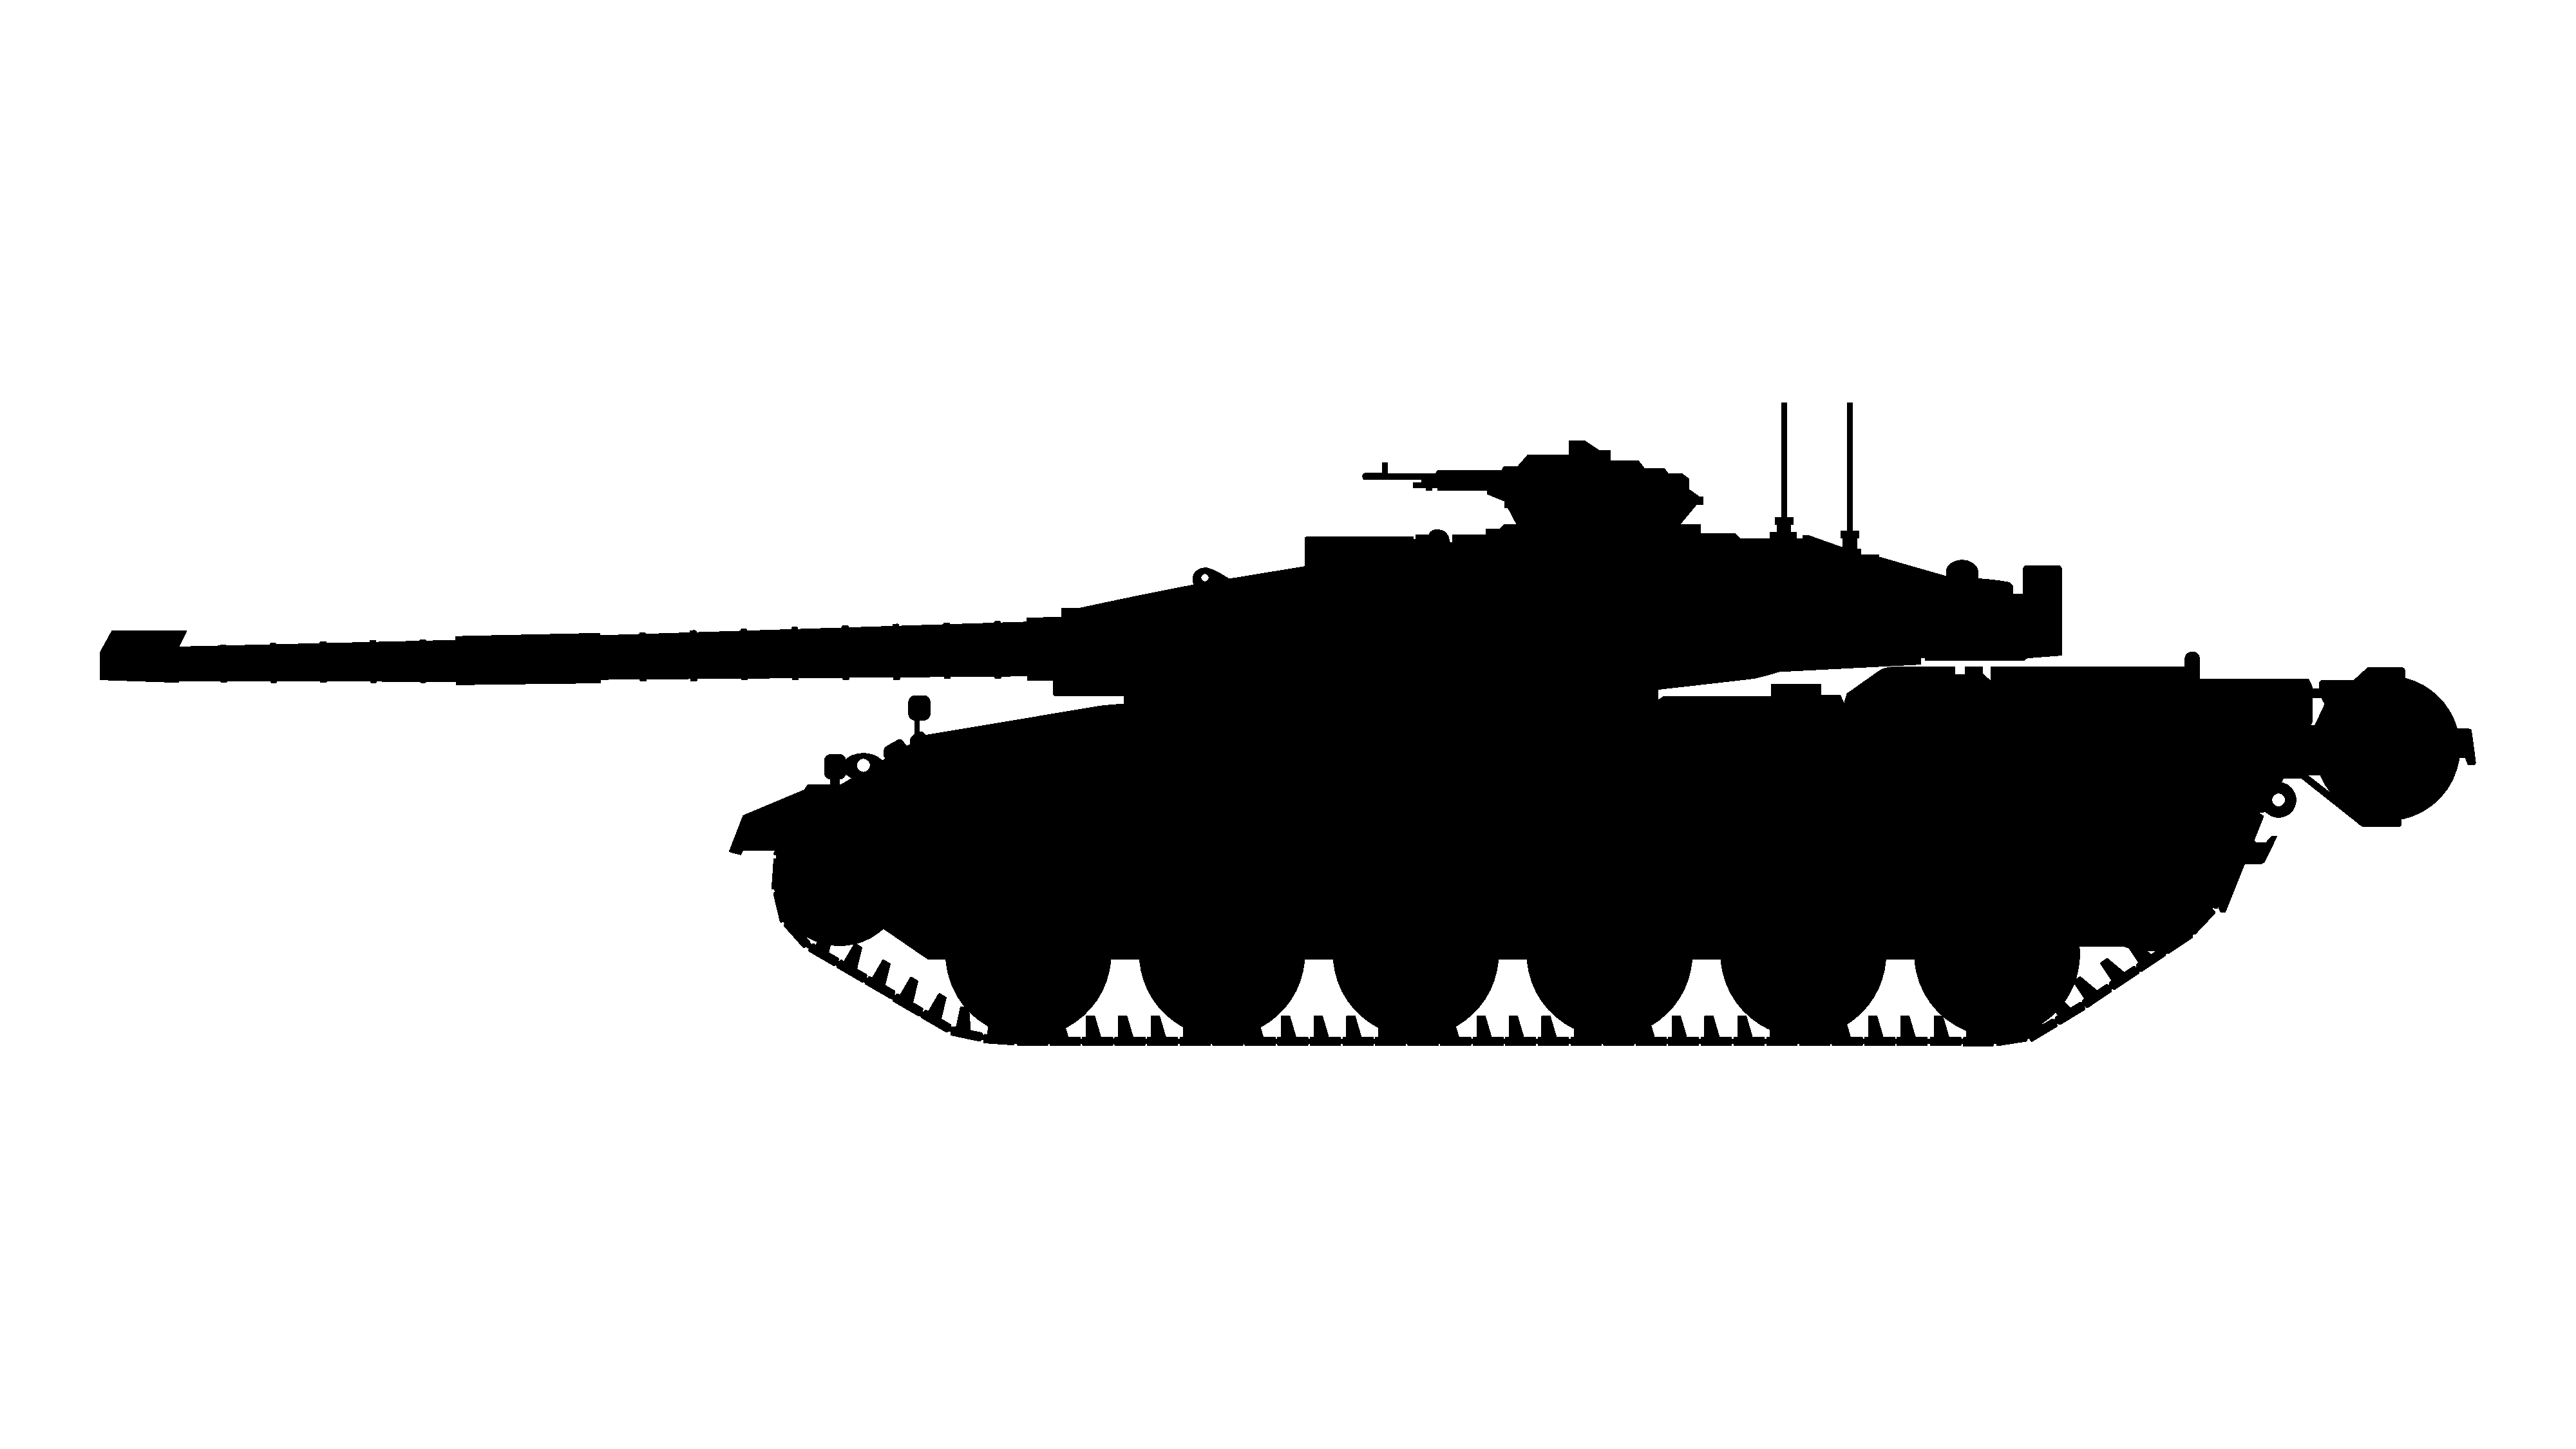
\includegraphics[width=0.6\textwidth]{platforms/challenger.pdf}
  \caption*{Challenger 2}
\end{figure}

\begin{figure}[h]
  \centering
  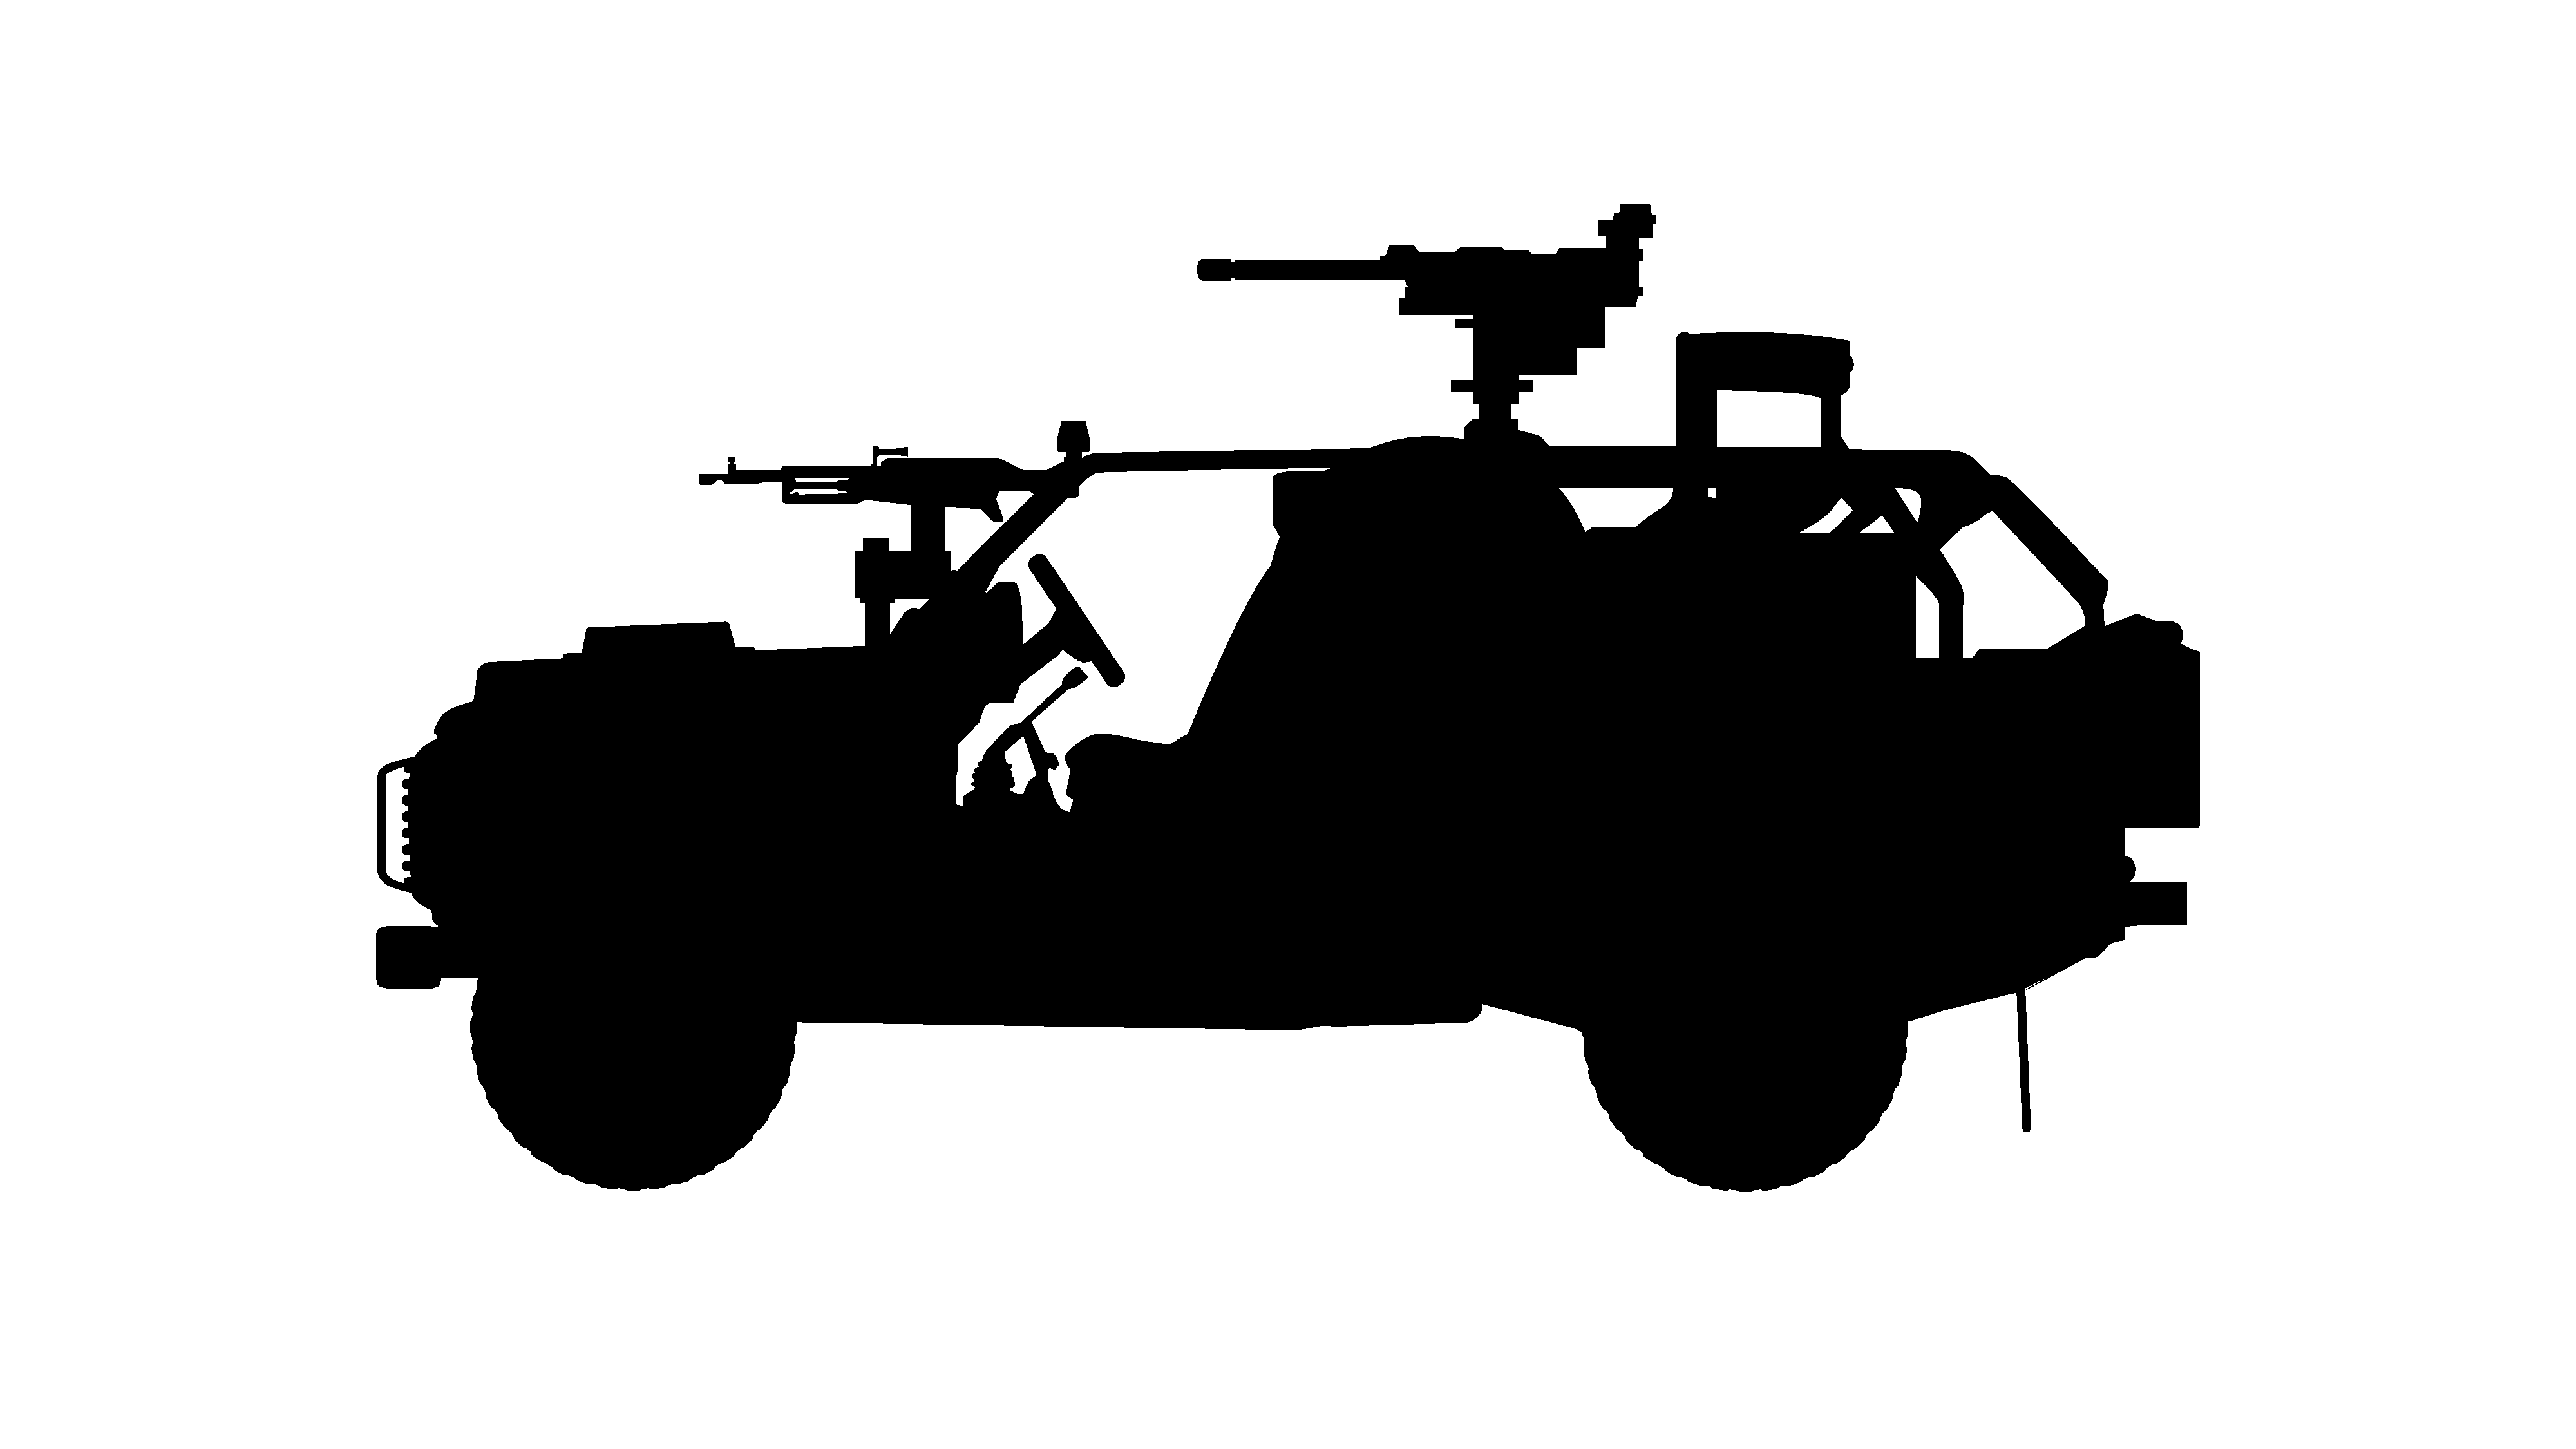
\includegraphics[width=0.6\textwidth]{platforms/wmik.pdf}
  \caption*{Land Rover Defender RWMIK}
\end{figure}

\begin{figure}[h]
  \centering
  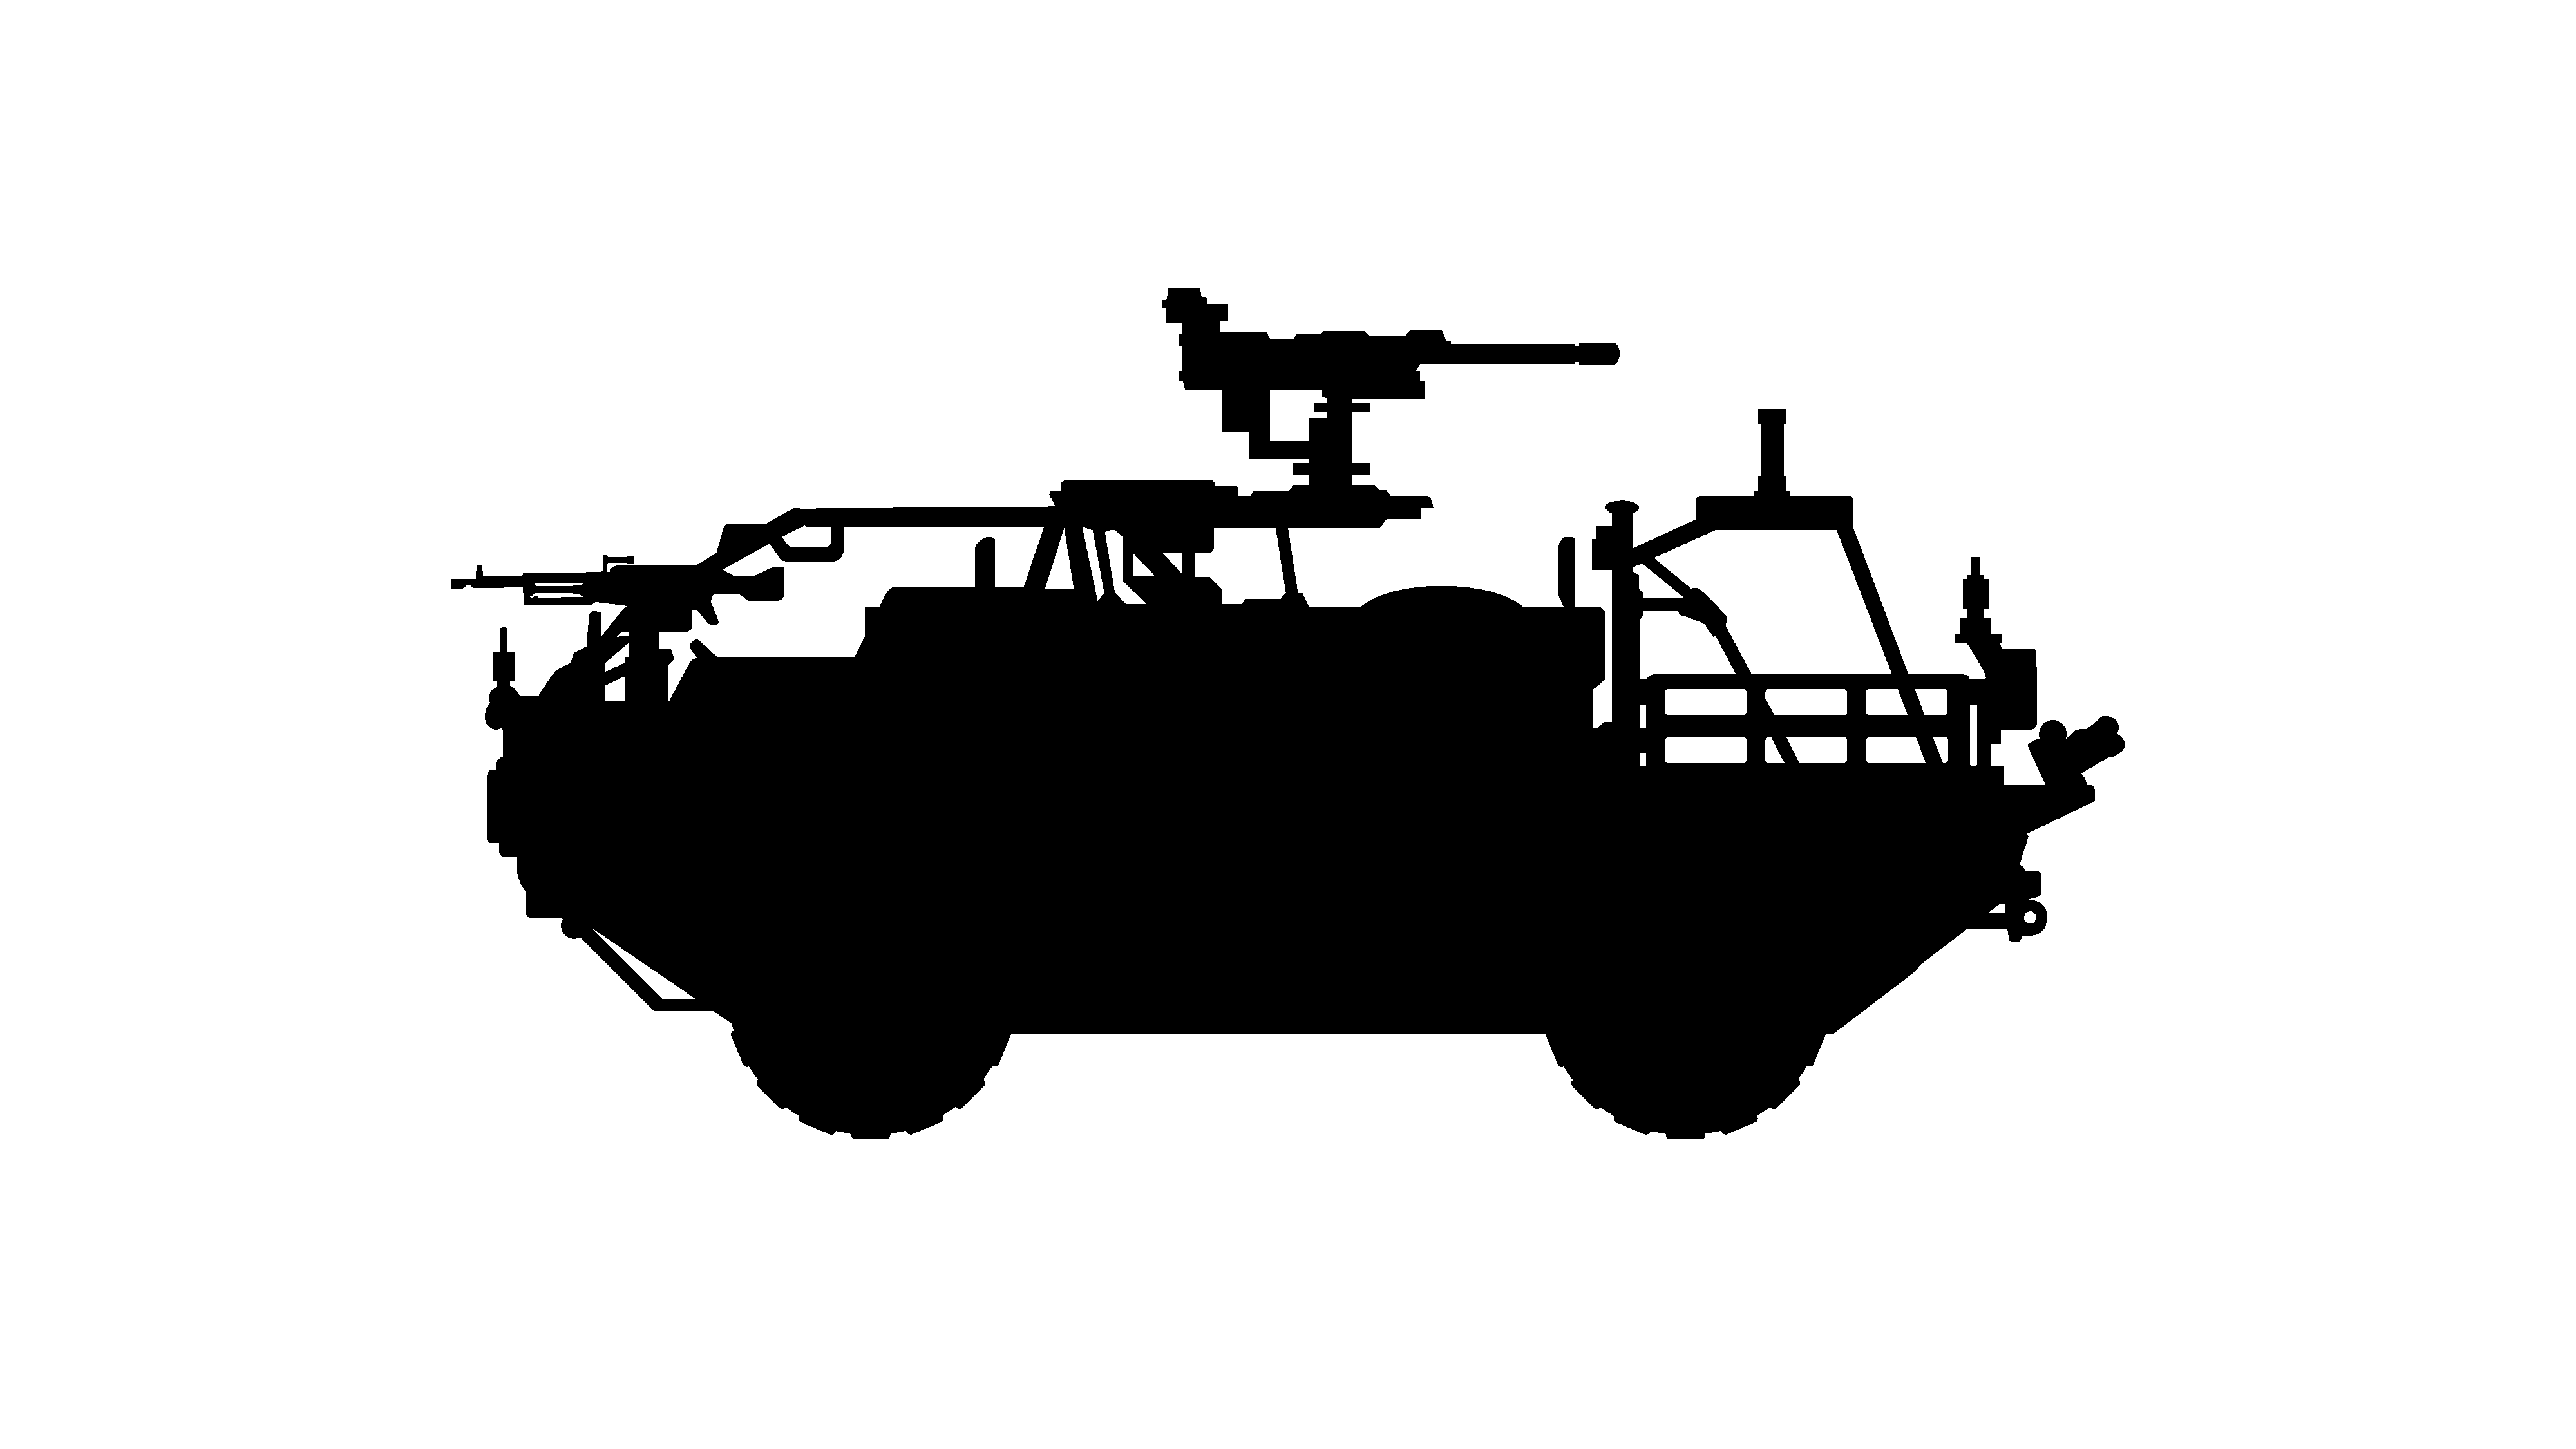
\includegraphics[width=0.6\textwidth]{platforms/jackal.pdf}
  \caption*{Supacat Jackal MWMIK}
\end{figure}


\chapter{Regimental March}

\poemtitle{D'ye ken John Peel}

\begin{verse}
\footnotesize
D'ye ken John Peel with his coat so gray? \\
D'ye ken John Peel at the break of the day? \\
D'ye ken John Peel when he's far, far away, \\
With his hounds and his horn in the morning?

\vin  'Twas the sound of his horn call'd me from my bed, \\
\vin  And the cry of his hounds has me oft-times led; \\
\vin  For Peel's view halloa would 'waken the dead, \\
\vin  Or a fax from his lair in the morning.

D'ye ken that bitch whose tongue is death? \\
D'ye ken her sons of peerless faith? \\
D'ye ken that a fox with his last breath \\
Curs'd them all as he died in the morning?

\vin  'Twas the sound of his horn call'd me from my bed...

Yes, I ken John Peel and auld Ruby, too, \\
Ranter and Royal and Bellman as true; \\
From the drag to the chase, from the chase to the view, \\
From the view to the death in the morning.

\vin  'Twas the sound of his horn call'd me from my bed...

And I've follow'd John Peel both often and far, \\
O'er the rasper-fence and the gate and the bar, \\
From Low Denton-holme up to the Scratchmere Scar, \\
When we vied for the brush in the morning.

\vin  'Twas the sound of his horn call'd me from my bed...

Then, here's to John Peel with my heart and soul, \\
Come fill--fill to him another strong bowl: \\
And we'll follow John Peel thro' fair and thro' foul \\
While we're wak'd by his horn in the morning.

\vin  'Twas the sound of his horn call'd me from my bed...
\end{verse}

\endgroup

\part{Journal}
\begingroup

\titleformat{\chapter}[display]{\Huge\bf}{}{0mm}{\centering}[]
\titlespacing{\chapter}{0mm}{0mm}{0mm}
\let\cleardoublepage\clearpage

\chapter{Prehistory}

\section*{1660s}

In the 1660s, in the reign of Charles II, there were records of two troops of volunteer Light Horse in the county of Cheshire. One record from 1660 describes a troop from the Hundreds\footnote{A \emph{hundred} is a subdivision of a county dating from before the Norman conquest - Cheshire had between seven and twelve hundreds at different times} of Wirral, Bucklow, and Macclsesfield, led by George Warburton, and a record from 1666 describes a troop from the hundreds of Broxton, Northwich, Nantwich, and Eddisbury\footnote{These are the modern names - contemporary records use \textit{Namptwich} and \textit{Edesbury}}, led by Lt~Col~Sir~Philip Egerton.

It's not clear how these troops connected at all to the later raising of the Cheshire Yeomanry proper, but the names associated with the two troops are familiar through the whole history of the Cheshire Yeomanry, including Cholmondeley, Egerton, Grosvenor, Wilbraham, and Warburton. It's notable that the two troops were led by an Egerton and a Warburton, and the last serving Ergerton-Warburton was in the Regiment as late as the 1960s.


\endgroup

\part{Encyclop{\ae}dia}
\small

\chapter*{B}

\section*{Bugle calls}

The Cheshire Yeomanry typically used the calls of the 5\nth Royal Inniskilling Dragoon Guards~\cite[p11]{trumpet-and-bugle-calls}, but also had their own trumpet and bugle calls.

\begin{figure}[h]
  \centering
  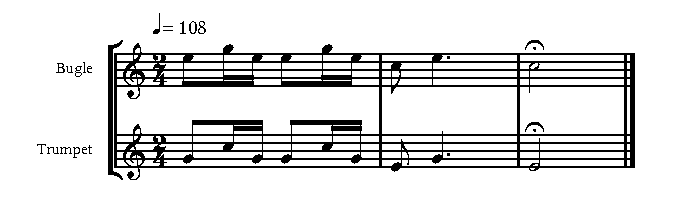
\includegraphics[width=0.75\textwidth]{gazette/cheshire-yeomanry-call.pdf}
  \caption*{Regimental call of the Cheshire Yeomanry~\cite[p11]{trumpet-and-bugle-calls}}
\end{figure}

\begin{figure}[h]
  \centering
  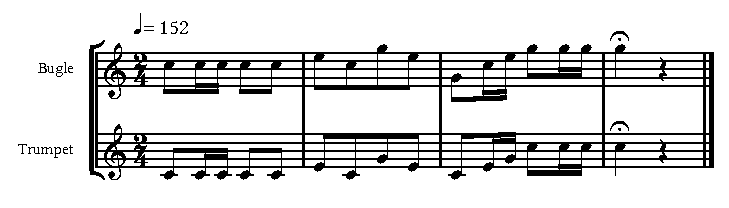
\includegraphics[width=0.75\textwidth]{gazette/5ridg-call.pdf}
  \caption*{Regimental call of the 5\nth Royal Inniskilling Dragoon Guards~\cite[p3]{trumpet-and-bugle-calls}}
\end{figure}

\chapter*{C}

\section*{Calls}

See \textit{bugle calls}.

\chapter*{T}

\section*{Trumpet calls}

See \textit{bugle calls}.


\part{Nominal Rolls}
\begingroup

\titleformat{\chapter}[display]{\Huge\bf}{}{0mm}{\centering}[]
\titlespacing{\chapter}{0mm}{0mm}{0mm}
\let\cleardoublepage\clearpage

\chapter*{1660}

\begin{center}
  \small
  \begin{tabular}{rl}
    Thomas, 3rd Earl Rivers & \\
    Lord Viscount Killmurry, and the Lady Killmur & William V \\
    Sir George Booth, Barronet & Samue Roe and Edward Delay \\
    Sir Willoby Aston, and those that enjoy Aston Landes & Thomas Hales \\
    George Warburton & \\
    Henry Brooke of Norton & John Barnes \\
    Thomas Manwaringe & Thomas Wainwright \\
    Thomas Brerton & John Houghe \\
    Thomas Maybury & William Rycroft \\
    Peter Leicester of nether Tabley & William Peacock \\
    John Leigh of Norbury Booths & Christopher Clay \\
    George Leicester of Tofte & Sussell Preston \\
    Peter Daniell of over Tabley, and his mother Mrs Danyell & Henry Antrobus \\
    Peter Brooke of Meire & George Ashton \\
    Henry Leigh of Heigh Leighe & William Gleaue \\
    Peter Leigh of Heigh Leighe & Peter R \\
    Edward Leigh of Baguley & \\
    Richard Marya Dumville of Limme and and Mrs Dumvile, Widow & Richard Lindall \\
    Starky of Stretton, Starky, and Jackson & \\
    William Tochett and Neither Whitly & \\
    Cholmonley of Holfor & Thomas Haukkins \\
    Harcott of Wyncham, Mouldsworth of Wyncham, and Peter Venables of Lostock & \\
    George Venables of Agdon & \\
    Richard Massy of Sale and Jeffery Cartwright & \\
    John Danyell of Dasbury and John Pickering & \\
    John Moores of Thelwall & \\
    Nathanyell Robinson, Lawrance Robinson, and Colthurst & Samuel Witter \\
    The Vikor of Budworth, the Vicar of Runckhorne, and Parson of Grappenhall & \\
    The Parson of Ashton upon Mercy Banke and Parsons of Limme and Warburton & \\
    The Parson of Mobberly, Vicar of Rosterne, and Vicar of Bowden & \\
  \end{tabular}
\end{center}




Men from:

The Bucklowe Hundred, formerly made of Trained Bands (Trained Bands are an earlier form of militia - these are possibly the earliest ancestors of the Cheshire Yeomanry?)
The Macclesfield Hundred
The Northwich Hundred
The Namptwich Hundred
The Boxton Hundred

\chapter*{1666}

\begin{center}
  \begin{tabular}{rl}
    Commander & Lt Col Sir Philip Egerton \\
    & Lt J Philips \\
    & Cnt C Cotton \\
    & Quartermaster W Brocke \\
    & Cpl Cumberbatch \\
    & Cpl Snell \\
    & Cpl Cooper \\
    & Trumpeter P Penckstone \\
    & Trumpeter W Ridway \\
    & Clerk F Adshed \\
  \end{tabular}
\end{center}

\begin{center}
  \Large
  \textbf{Broxton Hundred}
\end{center}

\begin{center}
  \small
  %\begin{tabular}{rl}
  \begin{tabular}{>{\raggedleft}m{5cm} m{5cm} }
    Lord Bishop of Chester & \dotfill \\
    Lord Cholmondeley & Francis Adshed and Randle Walker \\
    Sir Thomas Grosvenor & Richard Edwards \\
    The Lady Talbott & John Kellshall \\
    The Lady Calveley & Samuel Dickenson \\
    The heiress of Charles Walley & \dotfill \\
    Peter Dutton and Edward Bradshaw & Richard Tilston \\
    John Hurleston and William Brocke of Upton & Richard Willdigge \\
    The Parsons of Malpasee & Richard Cartwright \\
    Richard Alportt, Thomas Stockton, and John Catherall & John Steene \\
    Randle Dod, John Leech, George Bird & \\
    William Barneston, Edward Bromley, and Thomas Tanatt & Alex Cartwright \\
    Roger Puleston & George Morgan \\
    Henry Harpur, Edward Spencer, and Thomas Willcocks & William Sharman \\
    The Ministers of Waverton, Doddleston, Oldford, and Tattenhall & \dotfill \\
    The Deane and Chapter of Chester & \dotfill \\
  \end{tabular}
\end{center}

\pagebreak

\begin{center}
  \Large
  \textbf{Northwich Hundred}
\end{center}

\begin{center}
  \small
  \begin{tabular}{rl}
    Lord Brereton & \makecell[l]{Thomas Ashton, William Gorst, \\ John Cottingham} \\
    The Baron of Kinderton & \makecell[l]{John Millington, John Beayley, \\ and Joseph Venables} \\
    Sir John Bellott & John Hilditch \\
    Sir Jeffrey Shakerley & \dotfill \\
    Henry Mainwaringe & Samuel Bale \\
    George Davenport & John Snelson \\
    William Lawton, Thomas Smethwicke, \\ Somerfeild Oldfield, Archdale Palmer, \\ and Stephens of Wheelock & George Malbon \\
    Moreton of Hulme-Walfield, \\ John Ampson of Middlewich, Hone & George Wright \\
    The Parsons of Astbury, Warmincham, \\ and Davenham & Janies Statham \\
    The Lady Whittmoore, \\ Christopher Benon, Brookes & Henry Booth \\
  \end{tabular}
\end{center}

\begin{center}
  \Large
  \textbf{Namptwich Hundred}
\end{center}

\begin{center}
  \small
  \begin{tabular}{rl}
    Sir Thomas Wilbraham & Randel Fryar, Peter Cooke, and John Walton \\
    Sir Thomas Delves & Hugh Hampton, Thomas Reeve, Richard Own \\
    Sir Thomas Wainwaringe \\ and Sir Edward Minshull & Thomas Wainewright and John Bemisson \\
    Sir Thomas Smith & Richard Cooper \\
    Sir Robert Cotton & John Cleay \\
    George Vernon of Haslington & Thomas Price \\
    Roger Wilbraham of Darfold \\ and Roger Wilbraham of Namptwich & John Hatton and John Whittley \\
    Parson of Bartomley \\ and Vicar of Acton & \dotfill \\
  \end{tabular}
\end{center}

\pagebreak

\vspace*{30mm}

\begin{center}
  \Large
  \textbf{Edesbury Hundred}
\end{center}

\begin{center}
  \small
  \begin{tabular}{rl}
    Sir Philip Egerton & \dotfill \\
    Thomas Cholmondeley of Vale Royall & Thomas Billington and John Darlington \\
    John Crew of Vtkinton & John Golborne \\
    Chief Justice Bridgeman \\ and George Spurstowe & George Snell \\
    Thomas Lea and Mrs Warburton of Grange & John Tench \\
    Sir Peter Pindar, Jonathan Bruen, \\ and his son & John Johnson and John Beckett \\
    Darcy Savadge, \\ Mrs. Ann Moseley for Darley Hall & \dotfill \\
    George Davenport, \\ Mrs. Aldersey of Spurstowe, and Fradsham of Elton & John Pike \\
    Davies of Ashton, John Davies, \\ John Travers, and Wid' Hardware & Henry Gattliffe \\
  \end{tabular}
\end{center}

\vfill

\begin{center}
  \noindent
  \it
  \small
  Land owners are listed first, and then the riders they provided from their estates if their names are known.
\end{center}

\chapter*{1797}

\begin{center}
  \begin{tabular}{rl}
    Colonel Commandant & Col Sir John Leicester, later 1\st Baron de Tabley \\
    Commander & Lt Col T Dod \\
    & Maj T L Brooke \\
    & Capt C W J Sharkerley \\
    & Capt R Leycester \\
    & Capt H A Leicester \\
    & Lt L Page \\
    & Lt E Downes \\
    & Lt T Wright \\
    & Lt C D D Henchman \\
    & Lt C Antrobus \\
    & Cnt J Higginson \\
    & Cnt R Whitby \\
    & Cnt W Sutton \\
  \end{tabular}
\end{center}

\chapter*{1803}

\vspace*{10mm}

\begin{center}
  \Large
  \textbf{Earl of Chester's Regiment \\ of \\ Cheshire Yeomanry Cavalry}
\end{center}

\vspace*{10mm}

\begin{center}
  \begin{tabular}{rl}
    & Col Sir John Leicester, later 1\st Baron de Tabley \\
    & Lt Col T L Brooke \\
    & Maj H A Leicester \\
    Surgeon & P Holland \\
    Assistant-Surgeon & W Stone \\
    Adjutant & J Matchett \\
    Chaplain & Rev O Leycester \\
    & Capt R Leycester \\
    & Lt W Hollins \\
    & Cnt J Higginson \\
    & Capt E V Townshend \\
    & Lt J Davenport \\
    & Cnt W Okell \\
    & Capt B Ince \\
    & Lt T Ridgeway \\
    & Cnt J Shaw \\
    & Capt J S Daintry \\
    & Lt F Beswick \\
    & Cnt D Hall \\
    & Capt J Marshall \\
    & Lt H Furey \\
    & Cnt W Bradburn \\
  \end{tabular}
\end{center}

\vspace*{10mm}

\pagebreak

\vspace*{10mm}

\begin{center}
  \Large
  \textbf{Western Cheshire Volunteer Cavalry}
\end{center}

\vspace*{10mm}

\begin{center}
  \begin{tabular}{rl}
    & Lt Col Commandant T C Dod \\
    & Maj T Wild \\
    & Capt Sir John Stanley, 7\nth Baronet \\
    & Capt J Hill \\
    & Capt W H Worthington \\
    & Capt T Penson \\
    & Capt R Congreave \\
    & Capt J Richardson \\
    & Lt J Fielden \\
    & Lt H Potts \\
    & Lt T Fluitt \\
    & Lt F E Barker \\
    & Lt S Alderley \\
    & Cnt R Hill \\
    & Cnt J S Hughes \\
    & Cnt T Sudworth \\
    & Cnt J Bennion \\
    & Cnt W H Addison \\
    Chaplain & Rev T T Trevor \\
    Surgeon & G Harrison \\
  \end{tabular}
\end{center}

\chapter*{1804}

\vspace*{10mm}

\begin{center}
  \begin{tabular}{rl}
    & Col Sir J Leicester, later 1\st Baron de Tabley \\
    Adjt & J Matchett \\
  \end{tabular}
\end{center}

\vspace*{10mm}

\begin{center}
  \Large
  \textbf{Tabley Troop}
\end{center}

\vspace*{10mm}

\begin{multicols}{3}
  \small
  \noindent
  Quartermaster M Hulme \\
  Sgt W Ledward \\
  Sgt S Partington \\
  Sgt C Wallace \\
  Cpl J Hewit \\
  Cpl P Knowles \\
  Cpl W Partington \\
  Tptr J Blease \\
  Pte R Allen \\
  Pte J Bate \\
  Pte W Bayley \\
  Pte S Beecroft \\
  Pte W Beecroft \\
  Pte W Bradbury \\
  Pte T Brereton \\
  Pte P Broadhurst \\
  Pte S Carter \\
  Pte S Davenport \\
  Pte W Earls \\
  Pte T Evans \\
  Pte J Eaton \\
  Pte T Gleave \\
  Pte J Gleave \\
  Pte S Groves \\
  Pte J Golding \\
  Pte T Hewit \\
  Pte J Haslehurst \\
  Pte J Hickson \\
  Pte J Hewit \\
  Pte T Hickson \\
  Pte T Hough \\
  Pte J Haughton \\
  Pte T Jones \\
  Pte S Howard \\
  Pte W Lee \\
  Pte T Littler \\
  Pte C Lomas \\
  Pte J Hough \\
  Pte J Mann \\
  Pte S Meyers \\
  Pte J Meyers \\
  Pte J Moreton \\
  Pte G Noell \\
  Pte R Poole \\
  Pte J Steele \\
  Pte J Stretch \\
  Pte W Smith \\
  Pte P Stubbs \\
  Pte T Taylor \\
  Pte W Tasker \\
  Pte W Walton, Snr \\
  Pte W Walton, Jnr \\
  Pte T Warburton \\
  Pte J Witter \\
  Pte T Woodward \\
  Pte T Wyke \\
  Pte J Wyatt \\
\end{multicols}

\vspace*{10mm}

\pagebreak

\begin{center}
  \Large
  \textbf{Mere Troop}
\end{center}

\vspace*{10mm}

\begin{multicols}{3}
  \small
  \noindent
  Quartermaster R Cragg \\
  Sgt P Ashton \\
  Sgt J Okell \\
  Sgt R Broadbent \\
  Cpl J Blease \\
  Cpl M Crouchley \\
  Cpl J Pemberton \\
  Tptr T Burgess \\
  Pte J Ardern \\
  Pte S Ashbrooke \\
  Pte J Allen \\
  Pte J Ashton \\
  Pte S Barrow \\
  Pte W Broome \\
  Pte W Baguley \\
  Pte P Baguley \\
  Pte W Burrows \\
  Pte T Billington \\
  Pte J Bate \\
  Pte S Bradford \\
  Pte W Beecroft \\
  Pte J Cowsill \\
  Pte T Cragg \\
  Pte H Crouchley \\
  Pte D Dean \\
  Pte G Eden \\
  Pte T Eyres \\
  Pte W Fairclough \\
  Pte J Greaves \\
  Pte J Gleave \\
  Pte C Gleave \\
  Pte J Hampson \\
  Pte P Highfield \\
  Pte J Hamlett \\
  Pte T Hough \\
  Pte T Jon \\
  Pte W Jennings \\
  Pte D Kinsey \\
  Pte J Keeling \\
  Pte W Leigh \\
  Pte R Massey \\
  Pte J Millington \\
  Pte G Okell \\
  Pte W Partington \\
  Pte J Southern \\
  Pte T Swaine \\
  Pte J Toft \\
  Pte W Taylor \\
  Pte S Wright \\
  Pte W Whitley, Snr \\
  Pte W Whitley, Jnr \\
  Pte S Wilkinson \\
  Pte W Yould \\
  Pte W Powell \\
\end{multicols}

\vspace*{10mm}

\begin{center}
  \Large
  \textbf{Ashton Heyes Troop}
\end{center}

\vspace*{10mm}

\begin{multicols}{3}
  \small
  \noindent
  Quartermaster H Graham \\
  Sgt W Chatterton \\
  Sgt J Griffiths \\
  Sgt J White \\
  Cpl T Briscoe \\
  Cpl J Heath \\
  Cpl J Lewis \\
  Tptr W Jston \\
  Pte T Ankers \\
  Pte J Burgess \\
  Pte T Brookes \\
  Pte J Briscoe \\
  Pte J Bolland \\
  Pte W Cotgreve \\
  Pte J Cowap \\
  Pte J Cookson \\
  Pte W Clarke \\
  Pte W Dod \\
  Pte N Dod \\
  Pte J Dutton \\
  Pte J Done \\
  Pte T Es \\
  Pte J Gilbert \\
  Pte W Garner \\
  Pte R Harrison \\
  Pte S Hartbridge \\
  Pte E Jackson \\
  Pte C Jones \\
  Pte J Jones \\
  Pte T Jackson \\
  Pte W Jackson \\
  Pte R Lightfoot \\
  Pte J Lightfoot \\
  Pte J Lea \\
  Pte W Littler \\
  Pte J Lewis \\
  Pte T Musket \\
  Pte J Newhall \\
  Pte J Noden \\
  Pte B Pickering \\
  Pte W Peacock \\
  Pte W Robinson \\
  Pte W Reece \\
  Pte G Speakman \\
  Pte S Shaw \\
  Pte W Simmons \\
  Pte T Woodyer \\
  Pte J Walker \\
  Pte S Wilkinson \\
\end{multicols}

\vspace*{10mm}

\begin{center}
  \Large
  \textbf{Knutsford Troop}
\end{center}

\vspace*{10mm}

\begin{multicols}{3}
  \small
  \noindent
  Quartermaster I Taylor \\
  Sgt J Derbyshire \\
  Sgt J Lamb \\
  Sgt J Woodall \\
  Cpl J Burgess \\
  Cpl C Brandon \\
  Cpl J Dean \\
  Tptr G Hodges \\
  Pte J Acton \\
  Pte S Bailey \\
  Pte T Bradford \\
  Pte S Bradbury \\
  Pte J Bradford \\
  Pte H Birch \\
  Pte R Brown \\
  Pte I Baskerville \\
  Pte J Banks \\
  Pte T Boone \\
  Pte W Coldwell \\
  Pte J Cousell \\
  Pte J Clarke \\
  Pte R Craven \\
  Pte T Ditchfield \\
  Pte D Davies \\
  Pte H D \\
  Pte W Gatley \\
  Pte B Gratrix \\
  Pte J Gleave \\
  Pte W Hewit \\
  Pte J Howard \\
  Pte J Hodges \\
  Pte T Hussey \\
  Pte W Jordan \\
  Pte T Knowles \\
  Pte P Leather \\
  Pte J Lester \\
  Pte G Lee \\
  Pte J Lee \\
  Pte S Lee \\
  Pte J Leather \\
  Pte G Ecclestone \\
  Pte G Potter \\
  Pte S Plant \\
  Pte T Roylance \\
  Pte H Royle \\
  Pte T Rider \\
  Pte J Slater \\
  Pte P Street \\
  Pte W Swaine \\
  Pte S Siddeley \\
  Pte W Twiss \\
  Pte J Toft \\
  Pte S Wilson \\
  Pte P Wilkinson \\
  Pte J Witter \\
\end{multicols}

\vspace*{10mm}

\pagebreak

\begin{center}
  \Large
  \textbf{Macclesfield Troop}
\end{center}

\vspace*{10mm}

\begin{multicols}{3}
  \small
  \noindent
  Quartermaster M Tunnicliffe \\
  Sgt D Booth \\
  Sgt J Greaves \\
  Sgt J Rowbotham \\
  Cpl E Barrow \\
  Cpl S Bradbury \\
  Cpl C Mottershead \\
  Tptr H Shipton \\
  Pte W Ayton \\
  Pte C Ayton \\
  Pte T Arrowsmith \\
  Pte J Adshead \\
  Pte A Bay \\
  Pte J Barrow \\
  Pte J Bailey \\
  Pte J Bennett \\
  Pte T Booth \\
  Pte J Clewlowe \\
  Pte J Cook \\
  Pte T Critchley \\
  Pte E Cruttenden \\
  Pte W Davenport \\
  Pte E Fleet \\
  Pte J Greaves \\
  Pte T Goodwin \\
  Pte R Gaskell \\
  Pte S Hilditch \\
  Pte J Hodkinson \\
  Pte N Higginbotham \\
  Pte J Higginbotham \\
  Pte P Holland \\
  Pte T Hobson \\
  Pte S Henshall \\
  Pte R Kitsall \\
  Pte E Massey \\
  Pte J Massey \\
  Pte F Newbold \\
  Pte I Oliver \\
  Pte B Orme \\
  Pte T Phillips \\
  Pte G Pearson \\
  Pte E Rowe \\
  Pte S Stone \\
  Pte T Shaw \\
  Pte W Swann \\
  Pte W Scott \\
  Pte W Toft \\
  Pte R Turner \\
  Pte J Wright \\
  Pte W Waine \\
  Pte G Wood \\
  Pte T Wood \\
\end{multicols}

\vspace*{10mm}

\begin{center}
  \Large
  \textbf{Northwich Troop}
\end{center}

\vspace*{10mm}

\begin{multicols}{3}
  \small
  \noindent
  Quartermaster J Marshall \\
  Sgt T Antrobus \\
  Sgt H Jones \\
  Sgt T Oldham \\
  Cpl H Bennett \\
  Cpl J Molyneaux \\
  Cpl W Marrow \\
  Tptr C Dale \\
  Pte W Appleton \\
  Pte S Bradburn \\
  Pte R Bate \\
  Pte T Birch \\
  Pte T Barlow \\
  Pte W Beckett \\
  Pte W Bossen \\
  Pte T Chantler \\
  Pte W Dean \\
  Pte J Eauches \\
  Pte W Fowler \\
  Pte J Foster \\
  Pte S Grundy \\
  Pte J Hayes \\
  Pte C Holbrooke \\
  Pte J Hitchen \\
  Pte T Hodgkinson \\
  Pte W Holland \\
  Pte T Lawe \\
  Pte R Lownds \\
  Pte J Lovatt \\
  Pte R Littler \\
  Pte R Lambeth \\
  Pte J Minshell \\
  Pte J Moore \\
  Pte G Chesworth \\
  Pte J Ormson \\
  Pte J Oakes \\
  Pte J Olliver \\
  Pte G Prescott \\
  Pte J Rimmer \\
  Pte G Rotherham \\
  Pte T Shakeshaft \\
  Pte J Shepherd \\
  Pte J Tomkinson \\
  Pte D Thompson \\
  Pte T Wood \\
  Pte J Walmsley \\
  Pte W Wharton \\
  Pte R Wrench \\
  Pte J Woodcock \\
  Pte R Heath \\
  Pte J Roylance \\
  Pte J Ravenscroft \\
\end{multicols}

\chapter*{1810}

\begin{multicols}{2}
  \noindent
  Col Sir John Leicester, 1\nth Baron de Tabley \\
  Lt Col T Brooke \\
\end{multicols}

\begin{center}
  \Large
  \textbf{Tabley Troop}
\end{center}

\begin{multicols}{2}
  \noindent
  Capt R Leycester \\
  Lt W Hollins \\
  Cnt J Higginson \\
  Quartermaster M Hulme \\
  Sgt S Partington \\
  Sgt J Hewitt \\
  Sgt W Ledward \\
  Cpl P Knowles \\
  Cpl W Partington \\
  Cpl J Hough \\
  Tptr J Blease \\
  Farr R Allen \\
  Pte W Bradbury \\
  Pte S Carter \\
  Pte J Meyers \\
  Pte J Gleave \\
  Pte T Hickson \\
  Pte J Mann \\
  Pte J Moreton \\
  Pte T Smith \\
  Pte J Eaton \\
  Pte W Bailey \\
  Pte S Beecroft \\
  Pte T Brereton \\
  Pte G Davenport \\
  Pte T Gleave \\
  Pte C Knowles \\
  Pte S Meyers \\
  Pte P Stubbs \\
  Pte S Groves \\
  Pte J Goulding \\
  Pte J Haslehurst \\
  Pte J Steel, Snr \\
  Pte G Noell \\
  Pte J Taylor \\
  Pte J Woodward \\
  Pte C Earl \\
  Pte T Prescott \\
  Pte W Beecroft \\
  Pte T Evans \\
  Pte T Hewitt \\
  Pte J Hickson \\
  Pte W Tasker \\
  Pte T Wyke \\
  Pte P Wyatt \\
  Pte P Broadhurst \\
  Pte T Hough \\
  Pte P Foster \\
  Pte J Steel \\
  Pte J Gallimore \\
  Pte S Holbrooke \\
  Pte S Siddaley \\
  Pte J Simpson \\
  Pte I Williamson \\
  Pte W Nield \\
  Pte W Snelson \\
  Pte J Tomlin \\
  Pte T Blease \\
  Pte E Hayward \\
  Pte J Steel \\
  Pte W Eaton \\
  Pte R Holland \\
  Pte T Spragg \\
  Pte T Jackson \\
  Pte J Blease \\
  Pte R Clayton \\
  Pte T Mathers \\
\end{multicols}

\begin{center}
  \Large
  \textbf{Ashton Heyes Troop}
\end{center}

\begin{multicols}{2}
  \noindent
  Capt T Marshall \\
  Lt T Ridgway \\
  Cnt J Shaw \\
  Quartermaster J White \\
  Sgt J Lewis \\
  Sgt J Lewis \\
  Sgt W Littler \\
  Cpl J Briscoe \\
  Cpl J Dutton \\
  Cpl T Ankers \\
  Tptr W Johnson \\
  Pte J Cookson \\
  Pte W Dod \\
  Pte N Dod \\
  Pte T Edwards \\
  Pte T Jones \\
  Pte R Lightfoot \\
  Pte T Musket \\
  Pte W Peacock \\
  Pte W Robinson \\
  Pte W Reece \\
  Pte S Shaw \\
  Pte J Walker \\
  Pte W Clarke \\
  Pte J Burgess \\
  Pte B Pickering \\
  Pte J Lightfoot, Jnr \\
  Pte T Woodyer \\
  Pte R Harrison \\
  Pte G Lea \\
  Pte S Wilkinson \\
  Pte J Billington \\
  Pte J Dod \\
  Pte R Dentith \\
  Pte R Dykes \\
  Pte W Symonds \\
  Pte R Dilworth \\
  Pte J Goulborn \\
  Pte J Farrall \\
  Pte R Webster \\
  Pte S Hignet \\
  Pte J Bratt \\
  Pte S Adamson \\
  Pte E Briscoe \\
  Pte J Deane \\
  Pte J Dentith \\
  Pte S Harbridge \\
  Pte J Lightfoot \\
  Pte J Whitley \\
  Pte C Woodcock \\
  Pte J Cawley \\
  Pte T Peck \\
  Pte J Dutton \\
  Pte T Norton \\
  Farr T Roberts \\
  Pte W Harbridge \\
  Pte S Ball \\
  Pte J Newhall \\
\end{multicols}

\begin{center}
  \Large
  \textbf{Northwich Troop}
\end{center}

\begin{multicols}{2}
  \noindent
  Capt J Marshall \\
  Lt W Bradburne \\
  Cnt T Chantler \\
  Quartermaster T Antrobus \\
  Sgt J Molineux \\
  Sgt W Beckett \\
  Sgt D Thompson \\
  Cpl J Rylance \\
  Cpl J Yarwood \\
  Cpl S Bradburne \\
  Tptr R Lambeth \\
  Pte R Bate \\
  Pte T Birch \\
  Pte R Lownds \\
  Pte J Lovatt \\
  Pte J Eachers \\
  Pte J Hitchin \\
  Pte W Holland \\
  Pte J Moore \\
  Pte R Littler \\
  Pte J Ravenscroft \\
  Pte G Prescott \\
  Pte J Heyes \\
  Pte G Chesworth \\
  Pte S Heath \\
  Pte P Bancroft \\
  Pte H Smith \\
  Pte P Eaton \\
  Pte W Rhodes \\
  Pte A Riley \\
  Pte J Morris \\
  Pte W Goulding \\
  Pte J Brammall \\
  Pte R Wrench \\
  Pte T Winnington \\
  Pte J Horton \\
  Pte J Deakin \\
  Pte T Bate \\
  Pte R Holland \\
  Pte J Heald \\
  Pte S Barlow \\
  Pte G Warton \\
  Pte J Hartley \\
\end{multicols}

\begin{center}
  \Large
  \textbf{Knutsford Troop}
\end{center}

\begin{multicols}{2}
  \noindent
  Capt J Hollins \\
  Lt R Hancock \\
  Cnt F Sharpe \\
  Quartermaster I Taylor \\
  Sgt J Dean \\
  Sgt S Bailey, Jnr \\
  Sgt J Burgess, Jnr \\
  Cpl J Hodges \\
  Cpl W Pownall, Jnr \\
  Tptr G Hodges \\
  Farr J Leigh \\
  Pte J Acton \\
  Pte S Bradbury \\
  Pte T Ditchfield \\
  Pte J Howard \\
  Pte W Jordan \\
  Pte G Potter \\
  Pte J Slater \\
  Pte P Street \\
  Pte P Wilkinson \\
  Pte J Witter \\
  Pte H Birch \\
  Pte W Caldwell, Jnr \\
  Pte R Brown \\
  Pte S Siddeley \\
  Pte I Baskerville \\
  Pte J Banks \\
  Pte H Daniel \\
  Pte S Wilson \\
  Pte J Cowsill, Jnr \\
  Pte R Craven \\
  Pte J Leather \\
  Pte S Leigh \\
  Pte T Rider \\
  Pte W Swaine \\
  Pte J Gleave \\
  Pte J Bradford \\
  Pte J Clarke \\
  Pte P Leather \\
  Pte H Royle \\
  Pte B Gratrix \\
  Pte J Beade \\
  Pte T Hancock \\
  Pte T Clarke \\
  Pte S Birch \\
  Pte R Pigg \\
  Pte J Worthington \\
  Pte J Barratt \\
  Pte S Banks \\
  Pte S Wright \\
  Pte R Wright, Jnr \\
  Pte J Daniel \\
  Pte T Blackshaw \\
  Pte J Blackburn \\
  Pte J Parkes, Jnr \\
  Pte P Lee \\
  Pte W Higginson \\
  Pte J Roberts \\
\end{multicols}

\begin{center}
  \Large
  \textbf{Macclesfield Troop}
\end{center}

\begin{multicols}{2}
  \noindent
  Capt J S Daintry \\
  Lt D Hall \\
  Cnt H Critchley \\
  Quartermaster M Tunnicliffe \\
  Sgt D Booth \\
  Sgt E Barrow \\
  Sgt J Barrow \\
  Cpl C Mottershead \\
  Cpl J Adshead \\
  Cpl J Dale \\
  Farr J Findlow \\
  Tptr D Shipton \\
  Pte J Rowbotham \\
  Pte T Arrowsmith \\
  Pte T Critchley \\
  Pte J Cooke \\
  Pte J Hodgkinson \\
  Pte N Higginbotham \\
  Pte E Roe \\
  Pte S Stone \\
  Pte R Turner \\
  Pte G Wood \\
  Pte T Wood \\
  Pte J Dixon \\
  Pte J Newbold \\
  Pte H Ryle \\
  Pte N Percival \\
  Pte J Hardern \\
  Pte I Allen \\
  Pte J Bostock \\
  Pte J Davenport \\
  Pte R Broadhurst \\
  Pte A Bailey \\
  Pte C Greene \\
  Pte W Thorneycroft \\
  Pte J Whittaker \\
  Pte W Whittaker \\
  Pte T Grimsditch \\
  Pte W Low \\
  Pte T Wardle \\
  Pte S Grimsditch \\
  Pte M Grimsditch \\
  Pte C Bullock \\
  Pte S Orme \\
  Pte J Wilson \\
  Pte G Stringer \\
  Pte W Cantliff \\
  Pte J Barratt \\
  Pte E Johnson \\
  Pte J Frost \\
  Pte G Ridgway \\
  Pte C Turnock \\
  Pte W Radford \\
  Pte J Dale \\
  Pte E Lomas \\
  Pte J Swain \\
  Pte G Wright \\
  Pte T Johnson \\
\end{multicols}

\begin{center}
  \Large
  \textbf{Mere Troop}
\end{center}

\begin{multicols}{2}
  \noindent
  Capt E V Townshend \\
  Lt J Naylor \\
  Cnt W Okell \\
  Sgt J Okell \\
  Sgt P Ashton \\
  Sgt C Gleave \\
  Cpl J Pemberton \\
  Cpl M Crouchley \\
  Pte J Hampson \\
  Pte S Barrow \\
  Pte G Eden \\
  Pte S Wright \\
  Pte J Arden \\
  Pte J Cowsill \\
  Pte W Broom \\
  Pte W Partington \\
  Pte R Hickson \\
  Pte N Eden \\
  Pte J Eden \\
  Pte S Lamb \\
  Pte J Pownall \\
  Pte T Cragg \\
  Pte W Janing \\
  Pte J Burgess \\
  Pte R Bennett \\
  Pte W Baguley \\
  Pte H Drinkwater \\
  Pte J Allen \\
  Pte W Lee \\
  Pte P Baguley \\
  Pte W Taylor \\
  Pte J Ashton \\
  Pte J Southam \\
  Pte W Yould \\
  Pte W Burrows \\
  Pte T Swain \\
  Pte W Whitley \\
  Pte T Billington \\
  Pte T Massy \\
  Pte J Brocklow \\
  Pte J Wilkinson \\
  Pte W Bradford \\
  Pte T Hough \\
  Pte J Bradford \\
  Pte W Fairclough \\
  Pte T Jamieson \\
  Pte D Dean \\
  Pte T Hewitt \\
  Pte J Hewitt \\
  Pte S Basnett \\
  Pte T Kinsey \\
  Pte P Orme \\
  Pte W Povey \\
  Pte H Cronchley \\
  Pte J Millington \\
  Pte J Hamlett \\
  Pte S Wilkinson \\
  Tpr T Burgess \\
  Farr T Allen \\
\end{multicols}

\chapter*{1812}

\vspace*{10mm}

\begin{center}
  \textit{Only includes those deployed in aid of the civil power}
\end{center}

\vspace*{10mm}

\begin{center}
  \Large
  \textbf{Tabley Troop}
\end{center}

\begin{multicols}{3}
  \small
  \noindent
  Quartermaster M Hulme \\
  Sgt Ledward \\
  Sgt S Partington \\
  Sgt C Wallace \\
  Cpl J Hewitt \\
  Cpl P Knowles \\
  Cpl W Partington \\
  Tptr J Blease \\
  Pte R Allen \\
  Pte W Bayley \\
  Pte W Bancroft \\
  Pte T Brereton \\
  Pte P Broadbent \\
  Pte S Davenport \\
  Pte T Evans \\
  Pte J Eaton \\
  Pte T Gleave \\
  Pte J Gleave \\
  Pte S Groves \\
  Pte J Golding \\
  Pte T Hewit \\
  Pte J Haslehurst \\
  Pte J Hickson \\
  Pte T Hickson \\
  Pte T Hough \\
  Pte J Hough \\
  Pte J Mann \\
  Pte S Meyers \\
  Pte J Meyers \\
  Pte J Moreton \\
  Pte W Tasker \\
  Pte T Smith \\
  Pte T Wyke \\
  Pte J Taylor \\
  Pte C Earl \\
  Pte T Prescott \\
  Pte P Wyatt \\
  Pte P Foster \\
  Pte S Holbrooke \\
  Pte S Siddeley \\
  Pte J Williamson \\
  Pte J Carter \\
  Pte J Wright \\
  Pte T Hickson \\
  Pte Nixon \\
  Pte J Williamson \\
  Pte C Lowndes \\
  Pte J Gilgrass \\
  Pte Warburton \\
  Pte J Foden \\
\end{multicols}

\pagebreak

\vspace*{10mm}

\begin{center}
  \Large
  \textbf{Mere Troop}
\end{center}

\vspace*{10mm}

\begin{multicols}{3}
  \small
  \noindent
  Quartermaster R Cragg \\
  Sgt P Ashton \\
  Sgt J Okell \\
  Sgt C Gleave \\
  Cpl W Crouchley \\
  Tptr T Burgess \\
  Pte J Arden \\
  Pte J Allen \\
  Pte J Ashton \\
  Pte S Barrow \\
  Pte W Broome \\
  Pte W Baguley \\
  Pte P Baguley \\
  Pte W Burrows \\
  Pte T Billington \\
  Pte J Cowsill \\
  Pte T Cragg \\
  Pte D Dean \\
  Pte G Eden \\
  Pte T Eyres \\
  Pte W Fairclough \\
  Pte J Hampson \\
  Pte T Hough \\
  Pte T Jameson \\
  Pte W Jennings \\
  Pte W Leigh \\
  Pte J Millington \\
  Pte W Partington \\
  Pte T Swaine \\
  Pte S Wright \\
  Pte W Whitley, Snr \\
  Pte S Wilkinson \\
  Pte W Yould \\
  Pte J Pemberton \\
  Pte T Allen \\
  Pte S Lamb \\
  Pte S Barnett \\
  Pte W Hampson \\
  Pte T Massey \\
\end{multicols}

\vspace*{10mm}

\begin{center}
  \Large
  \textbf{Ashton Heyes}
\end{center}

\vspace*{10mm}

\begin{multicols}{3}
  \small
  \noindent
  Sgt J Lewis \\
  Sgt Briscoll \\
  Sgt W Litler \\
  Cpl T Ankers \\
  Tptr W Johnstone \\
  Pte J Burgess \\
  Pte W Dodd \\
  Pte N Dodd \\
  Pte J Dillon \\
  Pte T Edwards \\
  Pte J Gilbert \\
  Pte R Harrison \\
  Pte S Hartbridge \\
  Pte R Lightfoot \\
  Pte T Mushet \\
  Pte W Peacock \\
  Pte W Robinson \\
  Pte W Reece \\
  Pte S Shaw \\
  Pte W Simmons \\
  Pte T Woodyer \\
  Pte J Dentith \\
  Pte B Dickens \\
  Pte S Johnson \\
  Pte J Booth \\
  Pte T Woodcock \\
\end{multicols}

\vspace*{10mm}

\begin{center}
  \Large
  \textbf{Knutsford Troop}
\end{center}

\vspace*{10mm}

\begin{multicols}{2}
  \small
  \noindent
  Sgt John Dean \\
  Sgt S Bailey \\
  Cpl J Burgess \\
  Cpl J Hodges \\
  Cpl T Rider \\
  Farr J Lee \\
  Pte J Acton \\
  Pte H Birch \\
  Pte R Brown \\
  Pte J Baskerville \\
  Pte J Banks \\
  Pte W Caldwell \\
  Pte J Clarke \\
  Pte T Ditchfield \\
  Pte H Daniel \\
  Pte B Gratrix \\
  Pte J Gleave \\
  Pte J Howard \\
  Pte W Jordan \\
  Pte P Leather \\
  Pte G Potter \\
  Pte H Royle \\
  Pte J Slater \\
  Pte P Street \\
  Pte W Swaine \\
  Pte S Siddeley \\
  Pte S Wilson \\
  Pte P Wilkinson \\
  Pte J Sparks \\
  Pte J Leather \\
  Pte W Knowles \\
  Pte J Blackshaw \\
  Pte J Hewitt \\
  Pte S Blackshaw \\
\end{multicols}

\vspace*{10mm}

\begin{center}
  \Large
  \textbf{Macclesfield Troop}
\end{center}

\vspace*{10mm}

\begin{multicols}{2}
  \small
  \noindent
  Quartermaster M Tunnicliffe \\
  Sgt E Barrow \\
  Cpl J Adshead \\
  Tptr H Shipton \\
  Pte D Booth \\
  Pte T Arrowsmith \\
  Pte J Barrow \\
  Pte J Bailey \\
  Pte J Bennett \\
  Pte T Critchley \\
  Pte J Cook \\
  Pte J Hodkinson \\
  Pte N Higginbotham \\
  Pte T Hobson \\
  Pte E Massey \\
  Pte S Stone \\
  Pte R Turner \\
  Pte C Broadhurst \\
  Pte B Chear \\
  Pte J Goodwin \\
  Pte T Lomas \\
  Pte J Poole \\
  Pte R Potts \\
  Pte T Stringer \\
  Pte T Johnson \\
\end{multicols}

\vspace*{10mm}

\begin{center}
  \Large
  \textbf{Northwich Troop}
\end{center}

\vspace*{10mm}

\begin{multicols}{2}
  \small
  \noindent
  Sgt J Molineaux \\
  Sgt W Beckett \\
  Sgt D Thompson \\
  Cpl S Bradburn \\
  Tptr R Lambeth \\
  Pte R Bate \\
  Pte T Birch \\
  Pte J Hayes \\
  Pte J Hitchen \\
  Pte W Holland \\
  Pte J Lovatt \\
  Pte G Prescott \\
  Pte J Ravenscroft \\
  Pte W Bate \\
  Pte T Littler \\
  Pte J Mainwaring \\
  Pte T Eachus \\
  Pte C Leigh \\
  Pte W Golding \\
\end{multicols}

\chapter*{1814}

\begin{center}
  \textit{Only includes those deployed in aid of the civil power}
\end{center}

\begin{center}
  \Large
  \textbf{1st Macclesfield Troop}
\end{center}

\begin{multicols}{2}
  \noindent
  Quartermaster J Newbold \\
  Sgt C Bullock \\
  Sgt E Barrow \\
  Sgt J Dale \\
  Cpl J Leah \\
  Cpl T Mottershead \\
  Pte J Barratt \\
  Pte G Ridgeway \\
  Pte C Turnock \\
  Pte W Whittaker \\
  Pte T Grimsditch \\
  Pte T Wardle \\
  Pte S Grimsditch \\
  Pte T Grimsditch \\
  Pte J Rowbotham \\
  Pte H Ryle \\
  Pte J Swain \\
  Pte T Arrowsmith \\
  Pte J Barrow \\
  Pte J Bayley \\
  Pte J Cook \\
  Pte J Hodkinson \\
  Pte T Hobson \\
  Pte E Massey \\
  Pte T Swanwick, Snr \\
  Pte J Swanwick \\
  Pte T Swanwick, Jnr \\
  Pte J Swanwick \\
  Pte W Bent \\
  Pte G Wright \\
  Pte W Paulden \\
  Pte D Hadern \\
  Pte T Bayley \\
  Pte J Frost \\
  Pte C Greaves \\
  Pte H Verdon \\
  Pte J Sergeant \\
  Pte J Davenport \\
  Pte J Goodhall \\
  Pte S Sefton \\
  Pte J Brooks \\
  Pte J Dixon \\
  Pte T Barton \\
  Pte J Taylor \\
  Pte T Hope \\
  Pte J Cotterall \\
  Pte W Madew \\
  Pte J Corbishley \\
  Pte S Pointon \\
  Pte W Potts \\
  Pte J Braddock \\
  Pte J Collier \\
  Pte T Ainsworth \\
  Tptr C Buckley \\
  Farr C Booth \\
\end{multicols}

\begin{center}
  \Large
  \textbf{2nd Macclesfield Troop}
\end{center}

\begin{multicols}{2}
  \noindent
  Capt D Hall \\
  Lt J Stone \\
  Cnt R Turner \\
  Sgt E Johnson \\
  Sgt J Robinson \\
  Sgt W Anderton \\
  Pte T Bullock \\
  Pte W Whittaker \\
  Pte J Lomas \\
  Pte J Thorneycroft \\
  Pte P Blackshaw \\
  Pte S Atkinson \\
  Pte J Brindley \\
  Pte G Whittaker \\
  Pte J Henshaw \\
  Pte F Thompstone \\
  Pte I Thompstone \\
  Pte H Hanbury \\
  Pte J Hammond \\
  Pte J Bullock \\
  Pte E Gee \\
  Pte R Mottershead \\
  Pte T Trafford \\
  Pte J Davenport \\
  Pte T Davenport \\
  Pte J Goodfellow \\
  Pte A Filcock \\
  Pte T Harden \\
  Pte T Lockett \\
  Pte W Wincle \\
  Pte T Wincle \\
  Pte J Hamblet \\
  Pte G Redfern \\
  Pte J Booth \\
  Pte T Maden \\
  Pte W Robinson \\
  Pte T Hall \\
  Pte J Boothby \\
  Pte J Nixon \\
  Pte J Malkin \\
  Pte J Thorniley \\
  Pte G Burgess \\
  Pte B Chear \\
  Pte N Percival \\
  Pte J Harden \\
  Pte E Lomas \\
  Pte C Green \\
  Pte I Allen \\
  Pte J Bostock \\
  Pte R Broadhurst \\
  Pte J Whittaker \\
  Pte J Wilson \\
  Pte J Goodwin \\
  Pte J Poole \\
  Pte R Potts \\
  Pte T Stringer \\
  Tptr J Hall \\
  Farr J Findlow \\
\end{multicols}

\begin{center}
  \Large
  \textbf{Stockport Troop}
\end{center}

\begin{multicols}{2}
  \noindent
  Capt R Gee \\
  Lt R Roe \\
  Cnt J Newton \\
  Sgt T Garside \\
  Sgt J Howard \\
  Sgt T Foster \\
  Pte R Partington \\
  Pte E Thompson \\
  Pte S Stevenson \\
  Pte J Howard \\
  Pte J Radcliffe \\
  Pte E Sykes \\
  Pte R Fern \\
  Pte T Morton \\
  Pte T Steele \\
  Pte A Carrington \\
  Pte J Swindells \\
  Pte J Harrop \\
  Pte J Robinson \\
  Pte J Stringer \\
  Pte J Howard \\
  Pte J Lane \\
  Pte J Broadhurst \\
  Pte T Cartwright \\
  Pte W Brownhill \\
  Pte T Stanley \\
  Pte S Jowett \\
  Pte J Norbury \\
  Pte J Andrew \\
  Pte T Thorpe \\
  Pte P Wild \\
  Pte A Howard \\
  Pte H Howard \\
  Pte J Howard \\
  Pte J Barker \\
  Pte J Walmsley \\
  Pte J Bruckshaw \\
  Pte M Mayer \\
  Pte P Marsland \\
  Pte W Garman \\
  Pte E Taylor \\
  Pte H Lomas \\
  Pte D Shaw \\
  Pte W Clayton \\
  Pte J Hampson \\
  Pte J Isherwood \\
  Pte J Lidster \\
  Pte Howard \\
  Pte T Dicken \\
  Pte J Bolton \\
  Pte J Kinder \\
  Pte S Gaskell \\
  Pte J Bentley \\
\end{multicols}

\chapter*{1817}

\vspace*{10mm}

\begin{center}
  \textit{Only includes those deployed in aid of the civil power}
\end{center}

\vspace*{10mm}

\begin{center}
  \Large
  \textbf{Tabley Troop}
\end{center}

\begin{multicols}{3}
  \noindent
  Quartermaster Rose \\
  Sgt S Partington \\
  Sgt C Wallace \\
  Sgt J Haugh \\
  Cpl J Gleave \\
  Tptr W Mackenzie \\
  Pte W Bancroft \\
  Pte T Brereton \\
  Pte P Broadbent \\
  Pte S Groves \\
  Pte J Hickson \\
  Pte T Hough \\
  Pte J Mann \\
  Pte J Moreton \\
  Pte W Tasker \\
  Pte T Smith \\
  Pte T Wyke \\
  Pte C Earl \\
  Pte T Prescott \\
  Pte P Foster \\
  Pte J Steele, Snr \\
  Pte S Siddeley \\
  Pte W Sullivan \\
  Pte J Steele, Jnr \\
  Pte J Blease \\
  Pte R Clayton \\
  Pte J Burgess \\
  Pte J Gullimore \\
  Pte P Wyatt \\
  Pte T Whittaker \\
  Pte J Davies \\
  Pte T Banks \\
  Pte J Jackson \\
  Pte J Wilkinson \\
  Pte T Ledward \\
  Pte J Barlow \\
  Pte H Allen \\
  Pte J Law \\
  Pte P Barker \\
  Pte J Hewitt \\
  Pte W Barnard \\
  Pte J Forden \\
  Pte G Littler \\
  Pte J Singleton \\
  Pte J Stubbs \\
\end{multicols}

\chapter*{1818}

\vspace*{10mm}

\begin{center}
  \begin{tabular}{rl}
    & Col Sir John Leicester, 1\st Baron de Tabley \\
    & Lt Col E Townshend \\
  \end{tabular}
\end{center}

\vspace*{10mm}

\begin{center}
  \Large
  \textbf{Tabley Troop}
\end{center}

\begin{multicols}{3}
  \small
  \noindent
  Quartermaster W Rose \\
  Sgt S Partington \\
  Sgt W Bancroft \\
  Sgt J Hough \\
  Cpl T Hickson \\
  Tptr W Mackenzie \\
  Pte T Gleave \\
  Pte J Gleave \\
  Pte T Whittaker \\
  Pte J Haslehurst \\
  Pte C Earl \\
  Pte P Foster \\
  Pte J Blease \\
  Pte J Burgess \\
  Pte J Gallimore \\
  Pte J Davies \\
  Pte T Banks \\
  Pte J Jackson \\
  Pte J Barlow \\
  Pte H Allen \\
  Pte P Barber \\
  Pte J Hewitt \\
  Pte J Fordan \\
  Pte J Buckley \\
  Pte J Forster \\
  Pte T Hough \\
  Pte J Hickson \\
  Pte J Law \\
  Pte T Ledward \\
  Pte G Littler \\
  Pte C Lowndes \\
  Pte J Main \\
  Pte T Prescott \\
  Pte T Spragg \\
  Pte S Siddeley \\
  Pte W Snelson \\
  Pte J Steele, Snr \\
  Pte J Stubbs \\
  Pte J Singleton \\
  Pte J Steele, Jnr \\
  Pte W Foster \\
  Pte J Wright \\
  Pte T Wyke \\
  Pte P Wyatt \\
  Pte J Williamson \\
  Pte J Williamson \\
  Pte J Woodward \\
\end{multicols}

\vspace*{10mm}

\begin{center}
  \Large
  \textbf{Ashton Heyes Troop}
\end{center}

\begin{multicols}{3}
  \small
  \noindent
  Quartermaster J Lewis \\
  Sgt J Lewis \\
  Sgt R Briscoe \\
  Tptr W Johnson \\
  Pte J Briscoe \\
  Pte T Ankers \\
  Pte J Burgess \\
  Pte J Bratt \\
  Pte P Briscoe \\
  Pte J Booth \\
  Pte R Beckett \\
  Pte S Beckett \\
  Pte R Dentith \\
  Pte R Dilworth \\
  Pte J Dutton, Snr \\
  Pte J Dutton, Jnr \\
  Pte T Darlington \\
  Pte J Dentith \\
  Pte W Dickinson \\
  Pte S Cowan \\
  Pte W Ellis \\
  Pte J Finchitt \\
  Pte J Gilbert \\
  Pte S Gilbert \\
  Pte J Greenaway \\
  Pte R Harrison \\
  Pte J Hall \\
  Pte R Heath \\
  Pte S Johnson \\
  Pte J Johnson \\
  Pte J Jackson \\
  Pte J Jones \\
  Pte J Lightfoot \\
  Pte J Lightfoot, Jnr \\
  Pte J Lea \\
  Pte T Muskett \\
  Pte G Oulton \\
  Pte W Robinson \\
  Pte T Roberts \\
  Pte J Roberts \\
  Pte G Stockton \\
  Pte J Symmons \\
  Pte T Wright \\
  Pte A White \\
  Pte T Witton \\
  Pte T Worrall \\
  Pte J Fox \\
\end{multicols}

\vspace*{10mm}

\begin{center}
  \Large
  \textbf{Northwich Troop}
\end{center}

\begin{multicols}{3}
  \small
  \noindent
  Quartermaster \\ \indent T Antrobus \\
  Sgt J Molyneaux \\
  Sgt W Beckett \\
  Sgt D Thompson \\
  Tptr W Whitney \\
  Pte J Eachus \\
  Pte J Yarwood \\
  Pte J Morris \\
  Pte J Arrowsmith \\
  Pte R Wrench \\
  Pte R Bate \\
  Pte H Smith \\
  Pte H Hughes \\
  Pte T Foster \\
  Pte C Leigh \\
  Pte T Williams \\
  Pte J Horton \\
  Pte T Horton \\
  Pte J Mainwaring \\
  Pte J Ravenscroft \\
  Pte G Prescott, Jnr \\
  Pte R Littler \\
  Pte J Hesketh \\
  Pte C Wittingham \\
  Pte J Heald \\
  Pte R Ball \\
  Pte J Ainson \\
  Pte J Vernon \\
  Pte J Torbuck \\
  Pte R Wittingham \\
  Pte R Woodward \\
  Pte J Wild \\
  Pte S Austin \\
  Pte R Shaw \\
  Pte J Lythgoe \\
  Pte J Walker \\
  Pte C Berry \\
  Pte T Wild \\
  Pte J Davis \\
  Pte J Johnson \\
  Pte P Robinson \\
  Pte P Anderson \\
  Pte J Yardley \\
  Pte J Longshaw \\
  Pte W Miller \\
  Pte S Kinsey \\
  Pte T Woodyear, Jnr \\
  Pte J Yearsley \\
  Pte G Gleave \\
  Pte J Williams \\
  Pte W Wharton \\
  Pte W Dawson \\
  Pte T Bancroft \\
  Pte J Sanderson \\
  Pte S Eachus \\
  Pte T Warton \\
\end{multicols}

\pagebreak

\begin{center}
  \Large
  \textbf{Knutsford Troop}
\end{center}

\begin{multicols}{3}
  \small
  \noindent
  Quartermaster I Taylor \\
  Sgt J Dean \\
  Sgt S Bailey \\
  Sgt J Burgess \\
  Tptr G Hodges \\
  Pte J Acton \\
  Pte J Alderson \\
  Pte T Ditchfield \\
  Pte J Slater \\
  Pte P Wilkinson \\
  Pte J Howard \\
  Pte B Froggatt \\
  Pte J Read \\
  Pte P Street \\
  Pte P Hall \\
  Pte R Moore \\
  Pte R Howard \\
  Pte J Gaskell \\
  Pte S Forrester \\
  Pte G Potter \\
  Pte W Green \\
  Pte W Caldwell \\
  Pte H Birch \\
  Pte R Brown \\
  Pte S Wright \\
  Pte P Lee \\
  Pte J Royle, Jnr \\
  Pte W Pownall \\
  Pte W Higgins \\
  Pte J Worthington \\
  Pte J Bracegirdle \\
  Pte R Wright \\
  Pte J Daniels \\
  Pte S Wilson \\
  Pte S Siddeley \\
  Pte T Clarke, Jnr \\
  Pte H Daniels, Jnr \\
  Pte J Hope \\
  Pte S Hope \\
  Pte S Norbury \\
  Pte J Robinson \\
  Pte N Booth \\
  Pte W Shatwell \\
  Pte J Leigh \\
  Pte J Leather \\
  Pte W Twisse, Jnr \\
  Pte W Coleshill, Jnr \\
  Pte S Toft \\
  Pte J Clarke \\
  Pte J Henshall \\
  Pte H Royle \\
  Pte W Occlestone \\
  Pte I Baskerville \\
  Pte J Hodges \\
  Pte W Parkes \\
  Pte F Hancock, Jnr \\
  Pte A Walley \\
\end{multicols}

\vspace*{10mm}

\begin{center}
  \Large
  \textbf{1st Macclesfield Troop}
\end{center}

\begin{multicols}{3}
  \small
  \noindent
  Quartermaster J Newbold \\
  Sgt T Thompson \\
  Sgt E Barrow \\
  Sgt J Dale \\
  Tptr P Lomax \\
  Pte J Lea \\
  Pte T Mottershead \\
  Pte T Wardle \\
  Pte T Swanwick, Snr \\
  Pte T Swanwick, Jnr \\
  Pte J Swanwick \\
  Pte J Swanwick \\
  Pte S Lockett \\
  Pte W Lockett \\
  Pte W Paulden \\
  Pte D Harden \\
  Pte P Bullock \\
  Pte J Swain \\
  Pte J Barrett \\
  Pte J Frost \\
  Pte C Greaves \\
  Pte J Rushton \\
  Pte J Davenport \\
  Pte T Hobson \\
  Pte J Goodall \\
  Pte S Sefton \\
  Pte J Brookes \\
  Pte J Adshead \\
  Pte J Dixon \\
  Pte D Massey \\
  Pte E Massey \\
  Pte H Birchinall \\
  Pte R Cookson \\
  Pte J Alltree \\
  Pte J Johnstone, Snr \\
  Pte J Johnstone, Jnr \\
  Pte J Powell \\
  Pte J Davis \\
  Pte J Hulley \\
  Pte G Darby \\
  Pte E Cope \\
  Pte J Beaumont \\
  Pte T Jones \\
  Pte C Turnock \\
  Pte J Barrow \\
  Pte W Bent \\
  Pte C Boothby \\
  Pte T Hope \\
  Pte W Mayden \\
  Pte J Corbishley \\
  Pte S Grimsditch \\
  Pte M Grimsditch \\
  Pte S Stansfield \\
  Pte J Taylor \\
  Pte J Cottershill \\
  Pte J Warburton \\
  Pte J Astle \\
  Pte G Ainsworth \\
  Pte T Wooley \\
\end{multicols}

\vspace*{10mm}

\begin{center}
  \Large
  \textbf{2nd Macclesfield Troop}
\end{center}

\begin{multicols}{3}
  \small
  \noindent
  Sgt E Johnson \\
  Sgt J Dale \\
  Sgt W Anderton \\
  Tptr C Buckley \\
  Pte J Burgess \\
  Pte T Johnson \\
  Pte W Robinson \\
  Pte T Hall \\
  Pte T Barton \\
  Pte H Booth \\
  Pte J Hudson \\
  Pte W Malkin \\
  Pte W Johnson \\
  Pte H Kerr \\
  Pte J Poole \\
  Pte F Boothby \\
  Pte J Booth \\
  Pte J Massey \\
  Pte T Jones \\
  Pte J Nightingale \\
  Pte J Bradley \\
  Pte J Bailey \\
  Pte T Barber \\
  Pte T Goodwin \\
  Pte J Braddock \\
  Pte G Pickford \\
  Pte R Potts \\
  Pte J Norbury \\
  Pte G Burgess \\
  Pte J Robinson \\
  Pte J Whittaker \\
  Pte J Bailey \\
  Pte T Bullock \\
  Pte J Green \\
  Pte J Bullock \\
  Pte J Lomas \\
  Pte J Thorneycroft \\
  Pte J Thompson \\
  Pte R Mottershead \\
  Pte W Trafford \\
  Pte J Hammond \\
  Pte P Blackshaw \\
  Pte S Atkinson \\
  Pte E Lomas \\
  Pte N Percival \\
  Pte J Hardern \\
  Pte T Harden \\
  Pte W Davenport \\
  Pte J Davenport \\
  Pte J Goodfellow \\
  Pte A Filcock \\
  Pte T Lockett \\
  Pte W Warrington \\
  Pte J Casey \\
  Pte T Kitchen \\
  Pte W Lamb \\
  Pte J Priestnall \\
  Pte G Priestnall \\
\end{multicols}

\vspace*{10mm}

\begin{center}
  \Large
  \textbf{Mere Troop}
\end{center}

\begin{multicols}{3}
  \small
  \noindent
  Quartermaster P Ashton \\
  Sgt J Pemberton \\
  Sgt C Gleave \\
  Sgt M Crouchley \\
  Cpl P Orme \\
  Cpl G Eden \\
  Cpl S Wilkinson \\
  Tptr T Burgess \\
  Farr T Allen \\
  Pte J Arden \\
  Pte T Coleshill \\
  Pte J Brown \\
  Pte S Burrows \\
  Pte W Broome \\
  Pte S Lamb \\
  Pte J Eden \\
  Pte S Wright \\
  Pte J Hampson \\
  Pte N Eden \\
  Pte W Partington \\
  Pte J Pownall \\
  Pte J Robinson \\
  Pte G Occlestone \\
  Pte J Cragg \\
  Pte T Cragg \\
  Pte W Jennings \\
  Pte J Carter \\
  Pte J Allen \\
  Pte T Kinsey, Snr \\
  Pte T Kinsey, Jnr \\
  Pte T Eyres \\
  Pte J Gibson \\
  Pte J Risley \\
  Pte P Orme \\
  Pte W Leigh \\
  Pte P Baguley \\
  Pte T Gleave \\
  Pte G Okell \\
  Pte W Hanton \\
  Pte J Brockley \\
  Pte W Whitley \\
  Pte T Swain \\
  Pte J Wilkinson \\
  Pte T Massey \\
  Pte J Billington \\
  Pte W Yould \\
  Pte J Lewis \\
  Pte H Crouchley \\
  Pte J Millington \\
  Pte W Fairclough \\
  Pte J Bradford \\
  Pte T Hough \\
  Pte T Hatton \\
  Pte W Bradford \\
  Pte D Dean \\
  Pte P Whitley \\
  Pte W Swaine \\
  Pte R Greaves \\
  Pte J Gleave \\
\end{multicols}

\vspace*{10mm}

\begin{center}
  \Large
  \textbf{Stockport Troop}
\end{center}

\begin{multicols}{3}
  \small
  \noindent
  Quartermaster J Howard \\
  Sgt J Radcliffe \\
  Sgt B Brownhill \\
  Sgt S Hunt \\
  Cpl W Pearson \\
  Cpl G Williams \\
  Cpl S S Barratt \\
  Tptr G Cooke \\
  Pte J Jowett \\
  Pte J Barke \\
  Pte R Wright \\
  Pte J Hunt \\
  Pte J Heathcote \\
  Pte R Fogg \\
  Pte H Lomas \\
  Pte J Hankinson \\
  Pte J Gleave \\
  Pte J R Walker \\
  Pte J Brammall \\
  Pte J Dakin \\
  Pte J Robinson \\
  Pte J Gosling \\
  Pte J Dodge \\
  Pte J Robinson \\
  Pte S Taylor \\
  Pte P Jepson \\
  Pte R White \\
  Pte W Sidebottom \\
  Pte J Bolton \\
  Pte T Newton \\
  Pte J Perry, Jnr \\
  Pte W Booth \\
  Pte W Birch \\
  Pte J Shirt \\
  Pte J Barlow \\
  Pte G Burgess \\
  Pte J Howard \\
  Pte W Woodcock \\
  Pte J Fowler \\
  Pte C Brown \\
  Pte J Hibbert \\
  Pte J Heathcote \\
  Pte J Johnson \\
  Pte J Thatcher \\
  Pte J Walley \\
  Pte T Hulme \\
\end{multicols}

\chapter*{1819}

\vspace*{10mm}

\begin{center}
  \Large
  \textbf{Part of the Prince Regent's \\ Cheshire Volunteer Legion}
\end{center}

\vspace*{5mm}

\begin{center}
  \begin{tabular}{rl}
    & Maj Commandant S Wright \\
    & Capt J Holland \\
    & Capt J Cragg \\
    & Capt J Potter \\
    & Capt J Dumville \\
    & Lt S Hardy \\
    & Lt W Okell \\
    & Lt W Dean \\
    & Lt R Brown \\
    & Ensign T Hooley \\
    & Ensign W Wright \\
    & Ensign J Hulme \\
    & Ensign J Done \\
    Surgeon & W Billingham \\
  \end{tabular}
\end{center}

\vspace*{5mm}

\begin{multicols}{1}
  \noindent
  \textbf{Dunham Massey Troop} \\
  Capt W Egerton \\
  Lt T Hibbert \\
  Cnt J Davenport \\
  \\
  \\
  \textbf{Altrincham Troop} \\
  Capt Sir Harry Mainwaring\footnote{2\nd Baronet} \\
  Lt R L Trafford \\
  Cnt P D Finney \\
\end{multicols}

\chapter*{1820}

\vspace*{10mm}

\begin{center}
  \Large
  \textbf{Adlington Lancers}
\end{center}

\vspace*{10mm}

\begin{multicols}{2}
  \noindent
  E Massey \\
  J Swanwick \\
  J Priestnall \\
  G Bridnell \\
  W Lane \\
  T Kitchen \\
  T Barber \\
  J Bradley \\
  J Wagstaff \\
  J Hope \\
  J Newbold \\
  J Norris \\
  J Davenport \\
  W Wilde \\
  G Broster \\
  T Barber \\
  J Hunslet \\
  W Forster \\
  W Wood \\
  T Barber \\
  T Dickinson \\
  R Newton \\
  J Burgess \\
  H Taylor \\
  I Carter \\
  W Hall \\
  M Grimsditch \\
  T Carrington \\
  J H Beswick \\
  T Reddish \\
  J Chatham \\
  J Hulme \\
  J Toft \\
  J Alman \\
  S Wood \\
  S Clarke \\
  J Bayley \\
  S Grimsditch \\
  A Hatton \\
  J Sandbach \\
  T Darby \\
  G Burgess \\
  G Lawton \\
  T Ryle \\
  E Kinsey \\
\end{multicols}

\chapter*{1823}

\vspace*{10mm}

\begin{center}
  \Large
  \textbf{Knutsford Troop}
\end{center}

\vspace*{10mm}

\begin{multicols}{3}
  \small
  \noindent
  Quartermaster I Taylor \\
  Sgt J Dean \\
  Sgt J Burgess \\
  Sgt J Hodges \\
  Cpl J Howard \\
  Cpl W Pownall \\
  Cpl W Parks \\
  Tptr G Hodges \\
  Pte B Froggatt \\
  Pte W Green \\
  Pte R Cliff \\
  Pte W Coldwell \\
  Pte J Slater \\
  Pte J Ravenscroft \\
  Pte R Borrow \\
  Pte J Newton \\
  Pte W Burgess \\
  Pte W Heason \\
  Pte T Bertles \\
  Pte T Heath \\
  Pte T Ditchfield \\
  Pte J Acton \\
  Pte S Egerton \\
  Pte J Rollinson \\
  Pte J Ashton \\
  Pte J Caulton \\
  Pte W Shatwell \\
  Pte J Lockett \\
  Pte J Maddock \\
  Pte H Birch \\
  Pte J Hewitt \\
  Pte P Stubbs \\
  Pte S Worsley \\
  Pte H Daniel \\
  Pte J Daniel \\
  Pte J Hope \\
  Pte P Richardson \\
  Pte T Potter \\
  Pte S Norbury \\
  Pte J Wilson \\
  Pte C Wilson \\
  Pte C Hall \\
  Pte T Leech \\
  Pte R Wright \\
  Pte W Higginson \\
  Pte T Hancock \\
  Pte R Smith \\
  Pte H Royle \\
  Pte Ikin \\
  Pte P Street \\
  Pte T Austin \\
  Pte J Brown \\
  Pte J Leigh \\
  Pte Coleshill \\
  Pte J Twiss \\
\end{multicols}

\chapter*{1839}

\vspace*{10mm}

\begin{center}
  \textit{Only includes those deployed in aid of the civil power}
\end{center}

\vspace*{5mm}

\begin{center}
  \Large
  \textbf{Tatton Troop}
\end{center}

\begin{multicols}{3}
  \small
  \noindent
  Capt Tatton Egerton \\
  Lt Leycester \\
  Cnt Pownall \\
  Quartermaster John Howard \\
  Sgt Maj Kibble \\
  Sgt J Hope \\
  Sgt J Wilson \\
  Sgt T Newton \\
  Cpl J Dooley \\
  Cpl D Atkinson \\
  Tptr J Worthington \\
  Pte R Acton \\
  Pte J Ardern \\
  Pte J Batchelor \\
  Pte T Bartholomew \\
  Pte S Barrow \\
  Pte S Beech \\
  Pte J Bells \\
  Pte J Blackburn \\
  Pte J Blease \\
  Pte J Branson \\
  Pte W Broady \\
  Pte J Brown \\
  Pte W Brown \\
  Pte A Cash \\
  Pte J Cash \\
  Pte S Clarke \\
  Pte J Cunliffe \\
  Pte S Daniel \\
  Pte G Drinkwater \\
  Pte S Faulkner \\
  Pte H Gresty \\
  Pte W Hancock \\
  Pte J Hamilton \\
  Pte J Hampson \\
  Pte H Hope \\
  Pte P Hope \\
  Pte J Jackson \\
  Pte W Jennings \\
  Pte J Kinsey \\
  Pte J Lowndes \\
  Pte D Morris \\
  Pte J Palfrey \\
  Pte J Packs \\
  Pte W Partington \\
  Pte J Pickston \\
  Pte H Royle \\
  Pte P Richardson \\
  Pte T Shatwell \\
  Pte W Shuttleworth \\
  Pte G Suncock \\
  Pte P Stelfox \\
  Pte P Stockton \\
  Pte J Taylor \\
  Pte J Whitfield \\
  Pte R Wood, Snr \\
  Pte R Wood, Jnr \\
  Pte N Worsley \\
  Pte J Wright \\
\end{multicols}

\vspace*{10mm}

\pagebreak

\begin{center}
  \Large
  \textbf{Morley Troop}
\end{center}

\begin{multicols}{3}
  \small
  \noindent
  Capt H Trafford \\
  Quartermaster J Taylor \\
  Sgt O Lovell \\
  Sgt A Chadwick \\
  Cpl G Bannister \\
  Cpl W Massey \\
  Cpl J Hardman \\
  Farr R Oldfield \\
  Tptr J Lea \\
  Pte J Bradshaw \\
  Pte W Bradshaw \\
  Pte B Brundrett \\
  Pte P Chadwick, Snr \\
  Pte P Chadwick, Jnr \\
  Pte W Cowsell \\
  Pte S Faulkner \\
  Pte W Foster \\
  Pte R Gerrard \\
  Pte W Gibbon \\
  Pte W Gleave \\
  Pte J Hampson \\
  Pte B Hampson \\
  Pte N Hodcroft \\
  Pte S Hall \\
  Pte J Hulme \\
  Pte J Hulme \\
  Pte B Johnson \\
  Pte J Jolly \\
  Pte E Jones \\
  Pte J Ledger \\
  Pte J Lengard \\
  Pte J Lowe \\
  Pte W Mellor \\
  Pte J Mellor \\
  Pte T Massey \\
  Pte H Massey \\
  Pte L Matley \\
  Pte G Mellor \\
  Pte T Moss \\
  Pte J Parr \\
  Pte T Ogden \\
  Pte J Quin \\
  Pte S Rogers \\
  Pte J Royle \\
  Pte J Shawcross \\
  Pte H Sherlock \\
  Pte J Stainbank \\
  Pte T Stevens \\
  Pte A Holt \\
  Pte J Taylor \\
  Pte C Watson \\
  Pte T Williamson \\
  Pte J Whitehead \\
  Pte R Whittaker \\
  Pte R Wild \\
  Pte J Woodall \\
\end{multicols}

\vspace*{10mm}

\begin{center}
  \Large
  \textbf{Dunham Massey Troop}
\end{center}

\begin{multicols}{3}
  \small
  \noindent
  Sergeant Major Slater of Macclefield Squadron (attached) \\
  Capt T Worthington \\
  Lt T Wakefield \\
  Cnt H Thornton \\
  Quartermaster T Lotor \\
  Sgt T Cross \\
  Sgt P Davies \\
  Sgt J Hardy \\
  Cpl S Bancroft \\
  Cpl T Dean \\
  Cpl J Raines \\
  Tptr E Worthington \\
  Pte R Bowker \\
  Pte J Brown \\
  Pte G Clarke \\
  Pte J Cotterill \\
  Pte J Dawson \\
  Pte T Dudley \\
  Pte J Evans, Snr \\
  Pte J Evans, Jnr \\
  Pte T Foster \\
  Pte J Gallimore \\
  Pte R Gatley \\
  Pte J Goodier \\
  Pte J Gratrix \\
  Pte J Hampson \\
  Pte E Harrison \\
  Pte J Harrison \\
  Pte G Hobson \\
  Pte J Holt \\
  Pte T Howard \\
  Pte A Jackson \\
  Pte J Leigh \\
  Pte S Morris \\
  Pte J Perrin \\
  Pte P Shaw \\
  Pte T Stanbank \\
  Pte H Starkey, Snr \\
  Pte H Starkey, Jnr \\
  Pte S Timperley \\
  Pte J Walker \\
  Pte N Warburton \\
  Pte W Warburton \\
  Pte R Winkey \\
  Pte W Worthington \\
\end{multicols}

\vspace*{10mm}

\begin{center}
  \Large
  \textbf{Altrincham Troop}
\end{center}

\begin{multicols}{3}
  \small
  \noindent
  Lt Williams \\
  Cnt R Worthington \\
  Quartermaster W Worthington \\
  Sgt T Balshaw \\
  Sgt J Massey \\
  Sgt A Roberts \\
  Cpl E Hill \\
  Cpl J Story \\
  Cpl J Whittam \\
  Pte B Adshead \\
  Pte J Adshead \\
  Pte J Aldcroft \\
  Pte T Bailey \\
  Pte C Balshaw \\
  Pte B Chambers \\
  Pte J Clarke \\
  Pte C Ellison \\
  Pte J Goulden \\
  Pte R Hill \\
  Pte R Hargrave \\
  Pte P Holt \\
  Pte J Holt \\
  Pte W Harden \\
  Pte G Jackson \\
  Pte J Jones \\
  Pte N Jones \\
  Pte J Maire \\
  Pte J Perrin \\
  Pte W Perrin \\
  Pte S Pownall \\
  Pte J Pearson \\
  Pte J Rawlins \\
  Pte J Renshaw \\
  Pte N Royle \\
  Pte S Sheldon \\
  Pte I Timperley \\
  Pte J Warburton, Snr \\
  Pte J Wood \\
  Pte J Worthington \\
\end{multicols}

\begin{center}
  \Large
  \textbf{Macclesfield Troop}
\end{center}

\begin{multicols}{3}
  \small
  \noindent
  Capt J C Ryle \\
  Cnt Dod \\
  Quartermaster Gregory \\
  Sgt Pogmore \\
  Sgt Maydew \\
  Sgt Cundiffe \\
  Cpl Potts \\
  Cpl Bullock \\
  Cpl Gibbon \\
  Pte H Bailey \\
  Pte G Barton \\
  Pte E Bowers \\
  Pte T Boothby \\
  Pte C Chadwick \\
  Pte I Broom \\
  Pte T Coxon \\
  Pte J Cottrill \\
  Pte J Corbishley \\
  Pte W Dean \\
  Pte J Dumville \\
  Pte J Dale \\
  Pte J Dickin \\
  Pte W Hoult \\
  Pte J Holland \\
  Pte J Hibbert \\
  Pte J Hulse \\
  Pte R Johnson \\
  Pte J Latham \\
  Pte G Lancaster \\
  Pte W Lockett \\
  Pte R Middleton \\
  Pte S Orme \\
  Pte P B Pimlott \\
  Pte J Rathbone \\
  Pte W Scragg \\
  Pte T Simpson \\
  Pte A Thornley \\
  Pte A Whalley \\
  Pte J Wilshaw \\
  Pte J Wright \\
  Pte F Wood \\
  Pte W Walker \\
  Pte J Wardle \\
  Pte C Whiston \\
  Pte W Hanks \\
  Pte F Sefton \\
\end{multicols}

\pagebreak

\begin{center}
  \Large
  \textbf{Congleton Troop}
\end{center}

\begin{multicols}{3}
  \small
  \noindent
  Capt G C Antrobus \\
  Quartermaster J Newbold \\
  Sgt J Twiss \\
  Sgt J Hancock \\
  Sgt J Broadhurst \\
  Cpl Baddeley \\
  Cpl J Lomas \\
  Cpl G Lowe \\
  Pte J Astles \\
  Pte E Broad \\
  Pte R Burgess \\
  Pte J Brock \\
  Pte J Broadhead \\
  Pte C Bibby \\
  Pte C Blease \\
  Pte P Blackshaw \\
  Pte R Cowlishaw \\
  Pte J Deane \\
  Pte T Davenport \\
  Pte J Fenton \\
  Pte J Forster \\
  Pte W Ford \\
  Pte P Ford \\
  Pte J Fox \\
  Pte J Goodwin \\
  Pte D Heath \\
  Pte W Holland \\
  Pte R Sheratt \\
  Pte J Lownds \\
  Pte J Massey \\
  Pte J Oakes \\
  Pte W Slack \\
  Pte G Shrigley \\
  Pte J Shufflebotham \\
  Pte G Twemlow \\
  Pte P Ullivero \\
  Pte C Vaudrey \\
  Pte G Vernon \\
  Pte A Wright \\
  Pte E Wood \\
  Pte S Yates \\
  Pte J Lownds \\
\end{multicols}

\vspace*{10mm}

\begin{center}
  \Large
  \textbf{Stockport Troop}
\end{center}

\begin{multicols}{3}
  \small
  \noindent
  Capt Tatton \\
  Quartermaster I Shuttleworth \\
  Sgt Hardman \\
  Sgt E Barlow \\
  Sgt S Warren \\
  Cpl J Johnson \\
  Cpl J Fowler \\
  Cpl W Mundy \\
  Farr T Unsworth \\
  Tptr J Whittaker \\
  Pte J Antrobus \\
  Pte J Ardern \\
  Pte A Ashworth \\
  Pte G Bowers \\
  Pte J Bowers \\
  Pte E Bowers \\
  Pte J Bullock \\
  Pte C Cheteham \\
  Pte G Goodwin \\
  Pte G Gould \\
  Pte J Gouldshaw \\
  Pte T Higginbottom \\
  Pte W Hulme \\
  Pte W Hunt \\
  Pte S Jackson \\
  Pte H Norris \\
  Pte S Parry \\
  Pte J Shea \\
  Pte J Simister \\
  Pte T Smith \\
  Pte W Stanley \\
  Pte J Taylor \\
  Pte G Walker \\
  Pte J Walmsley \\
  Pte J Warmby \\
  Pte J Wood \\
  Pte T Worthington \\
  Pte T Woodard \\
  Pte T Kenyon \\
\end{multicols}

\chapter*{1842}

\vspace*{10mm}

\begin{center}
  \textit{Only includes those deployed in aid of the civil power}
\end{center}

\vspace*{10mm}

\begin{center}
  \Large
  \textbf{Tabley Troop}
\end{center}

\begin{multicols}{3}
  \small
  \noindent
  Capt Townshend \\
  Lt H Wallace \\
  Cnt W Worthington \\
  Quartermaster J Forster \\
  Sgt W Kibble \\
  Sgt J Steel \\
  Sgt T Blease \\
  Sgt J Cragg \\
  Cpl H Barber \\
  Cpl P Woodward \\
  Cpl T Morrey \\
  Tptr J Hulme \\
  Pte J Allen \\
  Pte J Ashbrooke \\
  Pte J Bentley \\
  Pte J Booth \\
  Pte S Blease \\
  Pte T Burgess \\
  Pte P Burgess \\
  Pte J Bowker \\
  Pte W Barber \\
  Pte J Carter \\
  Pte G Cawley \\
  Pte J Cockram \\
  Pte J Curbishley \\
  Pte J Cragg \\
  Pte R Earl \\
  Pte J Earl \\
  Pte J Forster \\
  Pte W Groves \\
  Pte T Groves \\
  Pte A Hewitt \\
  Pte P Hickson \\
  Pte J Hickson \\
  Pte T Hazlehurst \\
  Pte T Hough \\
  Pte J Hough \\
  Pte T Hurst \\
  Pte J Jackson \\
  Pte T Kynsey \\
  Pte W Leicester \\
  Pte J Lea \\
  Pte J Mann \\
  Pte J Manley \\
  Pte J Mosson \\
  Pte J Newton \\
  Pte J Platt \\
  Pte S Riley \\
  Pte J Smith \\
  Pte J Snelson \\
  Pte J Starkey \\
  Pte T Speakman \\
  Pte T Steel \\
  Pte S Tasker \\
  Pte T Venables \\
  Pte L Walley \\
  Pte W Yarwood \\
  Pte J Emson \\
\end{multicols}

\begin{center}
  \Large
  \textbf{Tatton Troop}
\end{center}

\begin{multicols}{3}
  \small
  \noindent
  Capt W T Egerton \\
  Cnt Pownall \\
  Quartermaster J Hope \\
  Sgt W Kibble \\
  Sgt J Wilson \\
  Sgt T Newton \\
  Sgt H Atkinson \\
  Cpl R Wood \\
  Cpl J Wright \\
  Cpl J Jackson \\
  Tptr J Worthington \\
  Pte J Acton \\
  Pte J Ardern \\
  Pte J Batchelor \\
  Pte S Barrow \\
  Pte J Bell \\
  Pte J Blackburn \\
  Pte J Bloor \\
  Pte S Bracegirdle \\
  Pte J Brown, Snr \\
  Pte J Brown, Jnr \\
  Pte W Brown \\
  Pte J Brown \\
  Pte J Brown \\
  Pte J Cash \\
  Pte S Clarke \\
  Pte J Cunliffe \\
  Pte J Daniel \\
  Pte S Faulkner \\
  Pte H Gresty \\
  Pte W Hancock \\
  Pte J Harrison \\
  Pte J Harrison \\
  Pte P Hewitt \\
  Pte H Hope \\
  Pte P Hope \\
  Pte J Jackson \\
  Pte J Jennings \\
  Pte J Jones \\
  Pte W Naden \\
  Pte J Kinsey \\
  Pte J Parks \\
  Pte W Partington \\
  Pte J Peckstone \\
  Pte H Royle \\
  Pte P Richardson \\
  Pte T Shatwell \\
  Pte G Simcock \\
  Pte J Skelhorn \\
  Pte P Stelfox \\
  Pte T Stelfox \\
  Pte P Stockton \\
  Pte R Wood \\
  Pte J Worthington \\
\end{multicols}

\vspace*{10mm}

\begin{center}
  \Large
  \textbf{Arley Troop}
\end{center}

\begin{multicols}{3}
  \small
  \noindent
  Lt Court \\
  Quartermaster P Carter \\
  Sgt J Walker \\
  Sgt G Smith \\
  Sgt S Wharton \\
  Sgt J Barker \\
  Cpl J Tickle \\
  Cpl G Artingstall \\
  Cpl R Richardson \\
  Tptr T Williams \\
  Pte W Beswick \\
  Pte J Barlow \\
  Pte S Barber \\
  Pte T Bennett \\
  Pte J Bradford \\
  Pte J Boardman \\
  Pte G Chadwick \\
  Pte J Cocker \\
  Pte J Darlington \\
  Pte J Dawson \\
  Pte J Dale \\
  Pte J Eachus \\
  Pte J Eden \\
  Pte E Grange \\
  Pte J Grange \\
  Pte J Holland, Snr \\
  Pte J Holland, Jnr \\
  Pte G Howes \\
  Pte J Haspel \\
  Pte T Harding \\
  Pte J Jones \\
  Pte W Lambert \\
  Pte R Lewis \\
  Pte J Mainwaring \\
  Pte H Maswell \\
  Pte J Miller \\
  Pte W Meredith \\
  Pte J Maddock \\
  Pte J Meire \\
  Pte G Moss \\
  Pte T Percival \\
  Pte J Robinson \\
  Pte T Robinson \\
  Pte J Smith \\
  Pte C Speakman \\
  Pte T Speakman \\
  Pte J Stockton \\
  Pte J Spruce \\
  Pte W Tomkinson \\
  Pte T Taylor \\
  Pte S Wright \\
  Pte J Yarwood \\
  Capt H Trafford \\
  Cnt S Raingill \\
  Quartermaster J Taylor \\
  Sgt O Lovell \\
  Sgt A Chadwick \\
  Cpl G Bannister \\
  Cpl W Massey \\
  Cpl J Jolly \\
  Pte J Ashcroft \\
  Pte W Axon \\
  Pte A Bannister \\
  Pte P Barber \\
  Pte J Bradshaw \\
  Pte W Bradshaw \\
  Pte B Brundritt \\
  Pte T Brundritt \\
  Pte J Chadwick \\
  Pte W Cowsell \\
  Pte W Foster \\
  Pte N Hodcroft \\
  Pte J Hodcroft \\
  Pte S Holt \\
  Pte J Hulme \\
  Pte J Hulme, Snr \\
  Pte J Hulme, Jnr \\
  Pte J Hulme \\
  Pte B Johnson \\
  Pte J Ledger \\
  Pte J Leigh \\
  Pte J Lingard \\
  Pte J Mallor \\
  Pte W Mallor \\
  Pte H Massey \\
  Pte T Massey \\
  Pte W Massey \\
  Pte G Mallor \\
  Pte T Moss \\
  Pte R Oldfield \\
  Pte T Ogden \\
  Pte J Parr \\
  Pte J Royle \\
  Pte J Shawcross \\
  Pte M Shawcross \\
  Pte H Sherlock \\
  Pte J Standbank \\
  Pte A Stott \\
  Pte J Taylor \\
  Pte R Wild \\
  Pte T Williamson \\
  Pte J Woodall \\
  Pte W Kibble \\
  Pte J Fielding \\
  Pte W Gleave \\
  Pte R Gerrard \\
  Pte J Grange \\
  Pte B Hampson \\
  Pte J Higham \\
  Pte J Higson \\
  Lt Palin \\
  Cnt Potts \\
  Quartermaster G Oulton \\
  Sgt J Walker \\
  Sgt R Southern \\
  Sgt W Steele \\
  Cpl S Rowe \\
  Cpl H Shuffiebotham \\
  Cpl W Jenkins \\
  Tptr J Elson \\
  Pte J Ankers \\
  Pte J Bottley \\
  Pte H Burgess \\
  Pte W Barnes \\
  Pte J Burrows \\
  Pte R Billington \\
  Pte W Beckett \\
  Pte C Clark \\
  Pte G Clark \\
  Pte J Crank \\
  Pte W Cowap \\
  Pte T Dodd \\
  Pte W Dutton, Snr \\
  Pte W Dutton, Jnr \\
  Pte W Gregory \\
  Pte W Johnson \\
  Pte J Jones \\
  Pte R Hewitt, Snr \\
  Pte R Hewitt Jun \\
  Pte R Hewitt, Snr \\
  Pte R Hewitt Jun \\
  Pte W Hitchins \\
  Pte G Hunt \\
  Pte J Hayward \\
  Pte T Livesley \\
  Pte S Lewis \\
  Pte T Norton \\
  Pte J Pennington \\
  Pte J Reece \\
  Pte J Rider \\
  Pte W Swinley \\
  Pte G Snelson \\
  Pte W Shaw \\
  Pte J Tepley \\
  Pte R Thomas \\
  Pte R Taylor \\
  Pte T Weaver \\
  Pte A White \\
  Pte S Whitlow \\
  Pte G Wood \\
  Pte W Warburton \\
  Pte G Wingfield \\
  Pte R Wade \\
  Pte S Walker \\
  Capt Leycester \\
  Lt Dod \\
  Cnt H Wright \\
  Quartermaster \\ \indent R B Maydew \\
  Sgt Marland \\
  Sgt Sefton \\
  Sgt Potts \\
  Cpl Gibbon \\
  Cpl Latham \\
  Cpl Whiston \\
  Tptr F Wood \\
  Pte Bullock \\
  Pte Simcock \\
  Pte Antrobus \\
  Pte Baguley \\
  Pte Broadhead \\
  Pte S Beswick \\
  Pte T Beswick \\
  Pte Bracegirdle \\
  Pte Fountain \\
  Pte Cockson \\
  Pte Cotrill \\
  Pte Daniel \\
  Pte Earl \\
  Pte Forest \\
  Pte Hatton \\
  Pte Holland \\
  Pte Hol \\
  Pte Hulse \\
  Pte J Beswick \\
  Pte Hankinson \\
  Pte Hodkinson \\
  Pte Kelsall \\
  Pte Massey \\
  Pte Middleton \\
  Pte Morris \\
  Pte Maybery \\
  Pte Levi Norbury \\
  Pte T Norbury \\
  Pte J Pearson \\
  Pte J Pownall \\
  Pte G Pownall \\
  Pte Simpson \\
  Pte J Simcock \\
  Pte Whalley \\
  Pte Willshaw \\
  Pte Wardle \\
  Pte Whitelegg \\
  Pte Walkley \\
  Pte Wood \\
  Pte J Whittaker \\
  Pte Williams \\
  Pte Featherstone \\
  Capt Antrobus \\
  Lt Reade \\
  Quartermaster J Twiss \\
  Sgt J Broadhurst \\
  Sgt G Lowe \\
  Sgt J Lomas \\
  Cpl W Baddeley \\
  Cpl S Yates \\
  Cpl P Ullivero \\
  Tptr G Barlow \\
  Pte J Astles \\
  Pte E Broad \\
  Pte R Burgess \\
  Pte J Baddeley \\
  Pte G Buckley \\
  Pte T Bailey \\
  Pte D Bailey, Snr \\
  Pte D Bailey, Jnr \\
  Pte R Burgess \\
  Pte C Blease \\
  Pte T Brightmore \\
  Pte J Davenport \\
  Pte R Cowlishaw \\
  Pte J Fenton \\
  Pte J Forster \\
  Pte W Forster \\
  Pte W Ford \\
  Pte J Fox \\
  Pte I Goodwin \\
  Pte D Heath \\
  Pte W Heath \\
  Pte W Holland \\
  Pte G Hawthorn \\
  Pte C Hickson \\
  Pte G Hughes \\
  Pte T Kelsall \\
  Pte T Lockett \\
  Pte W Lucas \\
  Pte J Massey \\
  Pte J Morris \\
  Pte J Perry \\
  Pte J Shufflebotham \\
  Pte J Shufflebotham \\
  Pte W Slack \\
  Pte W Smallwood \\
  Pte C Stubbs \\
  Pte F H Turner \\
  Pte G Vernon \\
  Pte A Wright \\
  Pte W Keeling \\
  Pte J Wareham \\
  Pte J Marland \\
  Pte J Siddall \\
  Pte T Lucas \\
  Pte J Blackshaw \\
  Pte T Fox \\
  Pte J Hobson \\
  Pte P Haslam \\
  Capt T W Tatton \\
  Lt E Marsland \\
  Quartermaster \\ \indent J Shuttleworth \\
  Sgt J Hardman \\
  Sgt J Johnson \\
  Sgt H Norris \\
  Cpl J Bullock \\
  Cpl J Chatham \\
  Cpl J Wild \\
  Tptr J Bowers \\
  Pte A Ashworth \\
  Pte J Bennet \\
  Pte I Booth \\
  Pte G Bowers \\
  Pte W Chadwick \\
  Pte J Cooke \\
  Pte J Cutler \\
  Pte A Curry \\
  Pte J Farmer \\
  Pte J Garner \\
  Pte J Gouldshaw \\
  Pte R Griffiths \\
  Pte R Harper \\
  Pte T Higginbotham \\
  Pte J Higginbotham \\
  Pte J Hunt \\
  Pte W Hunt \\
  Pte S Lomax \\
  Pte R Lovatt \\
  Pte W Marsland \\
  Pte G Mason \\
  Pte R Milton \\
  Pte T Morley \\
  Pte J Nield \\
  Pte S Parry \\
  Pte E Pearson \\
  Pte G Raynes \\
  Pte I Leah \\
  Pte J Redfern \\
  Pte J Robinson \\
  Pte P Royle \\
  Pte J Kidd \\
  Pte J Slack \\
  Pte W Stanley \\
  Pte J Walmsley \\
  Pte S Watkinson \\
  Pte R Warburton \\
  Pte G Wosingcroft \\
  Pte O Lovell \\
  Pte F Unsworth \\
\end{multicols}

\vspace*{10mm}

\begin{center}
  \Large
  \textbf{Dunham Massey Troop}
\end{center}

\begin{multicols}{3}
  \small
  \noindent
  Capt Worthington \\
  Lt Richmond \\
  Quartermaster N Pass \\
  Sgt A Roberts \\
  Sgt T Cross \\
  Sgt P Davies \\
  Sgt J Hardey \\
  Cpl S Bancroft \\
  Cpl J Reeves \\
  Tptr G Worthington \\
  Pte G Clarke \\
  Pte J Cottrill \\
  Pte H Daine \\
  Pte J Dawson \\
  Pte W Dawson \\
  Pte T Dudley \\
  Pte J Evans \\
  Pte J Galleymore \\
  Pte J Goodier \\
  Pte S Graham \\
  Pte E Harrison \\
  Pte G Hobson \\
  Pte T Hobson \\
  Pte J Holt \\
  Pte J Haslam \\
  Pte A Jackson \\
  Pte J Jackson \\
  Pte W Johnson \\
  Pte R Leather \\
  Pte S Morris \\
  Pte J Standbank \\
  Pte H Starkey, Snr \\
  Pte H Starkey, Jnr \\
  Pte I Timperley \\
  Pte J Thorpe \\
  Pte J Walker \\
  Pte W Warburton \\
  Pte N Warburton \\
  Pte R Winckley \\
  Pte W Worthington \\
  Capt Lloyd \\
  Lt Nicholson \\
  Quartermaster \\ \indent W Warburton \\
  Sgt T Balshaw \\
  Sgt S Gresty \\
  Sgt J Massey \\
  Cpl J Perrin \\
  Cpl J Whitlow \\
  Cpl A Roberts \\
  Tptr J Ackerley \\
  Pte J Aldcroft \\
  Pte B Adshead \\
  Pte J Adshead \\
  Pte C Balshaw \\
  Pte S Berry \\
  Pte J Clarke \\
  Pte J Clarke \\
  Pte H Drinkwater \\
  Pte J Goulden \\
  Pte W Greenwood \\
  Pte J Hewitt \\
  Pte J Holt \\
  Pte W Hardern \\
  Pte G Jackson \\
  Pte E Jackson \\
  Pte J Johnson \\
  Pte T Johnson \\
  Pte J Jones \\
  Pte N Jones \\
  Pte W Jones \\
  Pte T Norbury \\
  Pte J Pearson \\
  Pte S Pownall \\
  Pte J Rowland \\
  Pte J Renshaw \\
  Pte N Royle \\
  Pte S Sheldon \\
  Pte J Street \\
  Pte T Stubbs \\
  Pte J Sutton \\
  Pte I Timperley \\
  Pte W Walker \\
  Pte J Warburton, Snr \\
  Pte R Warburton \\
  Pte V Warburton \\
  Pte J Ward \\
  Pte J Worthington \\
  Pte J Weetman \\
\end{multicols}

\chapter*{1848}

\begin{center}
  \textit{Only includes those deployed in aid of the civil power}
\end{center}

\begin{center}
  \Large
  \textbf{Tabley Troop}
\end{center}

\begin{multicols}{2}
  \noindent
  Cnt W T Pownall \\
  Quartermaster J Hope \\
  Sgt J Wilson \\
  Sgt T Newton \\
  Sgt H Atkinson \\
  Sgt R Wood \\
  Cpl J Wright \\
  Cpl J Jackson \\
  Cpl I Taylor \\
  Cpl T Stelfox \\
  Pte R Acton \\
  Pte S Barrow \\
  Pte J Batchelor \\
  Pte J Bell \\
  Pte J Berry \\
  Pte J Blackburn \\
  Pte J Bloor \\
  Pte S Bracegirdle \\
  Pte W Bracegirdle \\
  Pte J Brown, Snr \\
  Pte W Brown \\
  Pte J Brown \\
  Pte J Cash \\
  Pte J Chadfield \\
  Pte S Clarke \\
  Pte J Cunliffe \\
  Pte J Davenport \\
  Pte I Erlam \\
  Pte S Faulkner \\
  Pte W Hancock \\
  Pte J Hardy \\
  Pte P Hewitt \\
  Pte H Hope, Snr \\
  Pte H Hope, Jnr \\
  Pte J Jennings \\
  Pte T Jones \\
  Pte J Kinsey \\
  Pte J Mason \\
  Pte J Mason \\
  Pte P Partington \\
  Pte J Pickstone \\
  Pte H Royle \\
  Pte G Simcock \\
  Pte J Stelfox \\
  Pte T Taylor \\
  Pte T Whittingham \\
  Pte J Wright, Snr \\
  Pte J Wright, Jnr \\
  Pte R Wood \\
  Pte J Wood \\
  Pte J Worthington \\
  Pte H Rogers \\
  Pte W Kibble \\
  Cnt S Pearson \\
  Sgt J Broadhurst \\
  Sgt G Lowe \\
  Sgt J Lomas \\
  Cpl S Yates \\
  Cpl P Ullivero \\
  Cpl P Haslam \\
  Farr C Blease \\
  Tptr T Green \\
  Pte J Astles \\
  Pte R Burgess \\
  Pte T Brightmore \\
  Pte J Baddeley \\
  Pte D Bailey \\
  Pte G Birtles \\
  Pte G Bunn \\
  Pte J Blackshaw \\
  Pte J Brocklehurst \\
  Pte R Cowlishaw \\
  Pte A Cope \\
  Pte W Cartlidge \\
  Pte J Dale \\
  Pte W Forster \\
  Pte T Ford \\
  Pte J Fox \\
  Pte I Goodwin \\
  Pte F Heath \\
  Pte W Holland \\
  Pte C Hickson \\
  Pte G Hughes \\
  Pte T Hackney \\
  Pte G Hill \\
  Pte T Kelsall \\
  Pte W Keeling \\
  Pte W Machin \\
  Pte E Massey \\
  Pte J M'Gannon \\
  Pte T Potts \\
  Pte J Peney \\
  Pte W Smallwood \\
  Pte J Siddall \\
  Pte J Stubbs \\
  Pte J Shropshale \\
  Pte F Turner \\
  Pte T Thorneycroft, Snr \\
  Pte T Thorneycroft, Jnr \\
  Pte J Wilde \\
  Pte W Drakeford \\
  Pte T Wright, Jnr \\
  Pte W Brittain \\
  Pte T Filcock \\
  Pte T Bailey \\
\end{multicols}

\chapter*{1897}

\begin{center}
  \begin{tabular}{rl}
    Hon Col & Lt Col H Grosvenor, 1\st Duke of Westminster \\
    Lt Col Comdt & Lt Col P Egerton-Warburton \\
    Major & Lt Col C A Stanhope, 8\nth Earl of Harrington \\
    Adjutant & Capt H P Kirkpatrick (16L) \\
    Surgeon & G Garrison \\
    Veterinary Surgeon & R E Edwards \\
    Bandmaster & J Clement \\
    RSM & G Cooper \\
  \end{tabular}
\end{center}

\begin{center}
  \Large
  \textbf{A (Tatton) Squadron}
\end{center}

\begin{multicols}{2}
  \noindent
  Sergeant Major D Souden \\
  Capt A de Tatton Egerton \\
  2Lt R C Parr \\
  Quartermaster C Sherwin \\
  Sgt J Newton \\
  Sgt W Chorlton \\
  Sgt J Brown \\
  Sgt W Pownall \\
  Cpl W Hope \\
  Cpl W Latham \\
  Cpl A Stellfox \\
  Cpl T Brown \\
  Farr L Newton \\
  Tptr W Brown \\
  Bandsman A Brannan \\
  Bandsman E Brannan \\
  Pte W Baguley \\
  Pte J Beswick \\
  Pte W Blackburn \\
  Pte W Booth \\
  Pte J Brown \\
  Pte T Burgess \\
  Pte A Daniels \\
  Pte W Ellison \\
  Pte C Erlam \\
  Pte I Erlam \\
  Pte O Garner \\
  Pte J C Gill \\
  Pte E Gresty \\
  Pte G Harrison \\
  Pte E Harrison \\
  Pte F Hope \\
  Pte J Hulme \\
  Pte J Jepson \\
  Pte J Johnson \\
  Pte C A Jones \\
  Pte G Leech \\
  Pte H Ourend \\
  Pte H Overend \\
  Pte R Sproston \\
  Pte T Stellfox \\
  Pte E Stockton \\
  Pte H T Stockton \\
  Pte J Warburton \\
  Pte S Warburton \\
  Pte S Whalley \\
  Pte J Whitelegge \\
  Capt H A Birley \\
  Lt R W D Phillips \\
  Quartermaster J Mason \\
  Sgt W Leech \\
  Sgt B Wright \\
  Sgt W Platt \\
  Cpl J Hewitt \\
  Cpl P Hewitt \\
  Cpl S Dale \\
  Cpl G Lee \\
  Bandsman G Driver \\
  Bandsman C Hopewell \\
  Pte W Barber \\
  Pte J Bloor \\
  Pte C Bowers \\
  Pte W Bracegirdle \\
  Pte J Bracegirdle \\
  Pte G Chorlton \\
  Pte C N Hewess \\
  Pte E Hollinsworth \\
  Pte J Hope \\
  Pte R Knowles \\
  Pte R Lloyd \\
  Pte R Moore \\
  Pte F Shrieves \\
  Pte J Stanier \\
  Pte G Stamer \\
  Pte T Steel \\
  Pte W Stockton \\
  Pte W Stockton \\
  Pte J Webb \\
  Pte S Webster \\
  Pte H Wilson \\
  Pte J Worthington \\
  Pte J Wright \\
  Pte S Wright \\
\end{multicols}

\begin{center}
  \Large
  \textbf{B (Eaton) Squadron}
\end{center}

\begin{multicols}{2}
  \noindent
  Sergeant Major W Bagg \\
  Capt Lord Arthur Grosvenor \\
  Lt E W Swetenham \\
  Quartermaster Allwood \\
  Sgt R Evans \\
  Sgt J Hartshorn \\
  Sgt G Mullock \\
  Cpl H Denson \\
  Cpl M Rowe \\
  Cpl E Cookson \\
  Cpl W Gillham \\
  Farr J Bramall \\
  Tptr A Myers \\
  Bandsman F Richardson \\
  Bandsman T Wardle \\
  Pte A Barker \\
  Pte H Cuzner \\
  Pte A Fearnall \\
  Pte W Fox \\
  Pte J Hewson \\
  Pte E Jones \\
  Pte R Jones \\
  Pte E Lloyd \\
  Pte G Lloyd \\
  Pte W Minshull \\
  Pte S Moore \\
  Pte J Mitchell \\
  Pte R Parry \\
  Pte J Parker \\
  Pte E Parting \\
  Pte T Partington \\
  Pte A Pickering \\
  Pte F Pickering \\
  Pte E Randles \\
  Pte J Rigby \\
  Pte W Roberts \\
  Pte W Wynne \\
  Pte B Youd \\
  Capt G Wyndham \\
  Lt H Barnston \\
  Quartermaster R Mullock \\
  Sgt R Walley \\
  Sgt J Gregory \\
  Sgt F Allwood \\
  Cpl F Wright \\
  Cpl S Partington \\
  Farr/Sgt S Palin \\
  Tptr J Lunt \\
  Bandsman A Baker \\
  Bandsman M Baker \\
  Pte J Allwood \\
  Pte F Caswell \\
  Pte C Corson \\
  Pte S Denson \\
  Pte J Dutton \\
  Pte G Emmerson \\
  Pte T Fearnall \\
  Pte J Grace \\
  Pte C Jones \\
  Pte T Jones \\
  Pte F Lake \\
  Pte W Lee \\
  Pte E Lewis \\
  Pte J Myers \\
  Pte S Minshull \\
  Pte T Minshull \\
  Pte C Moore \\
  Pte R Poynton \\
  Pte H Pritchard \\
  Pte J Pritchard \\
  Pte J Roberts \\
  Pte J Salmon \\
  Pte R Shepherd \\
  Pte G Thomas \\
  Pte C Walley \\
  Pte R Watkins \\
\end{multicols}

\begin{center}
  \Large
  \textbf{C Squadron (Arley and Bostock Troops)}
\end{center}

\begin{multicols}{2}
  \noindent
  Sergeant Major W Barret \\
  Capt O M Leigh \\
  2Lt H M Wilson \\
  Quartermaster R Hornby \\
  Sgt R Clarke \\
  Sgt T Williamson \\
  Sgt J Lambert \\
  Cpl J Whitlow \\
  Cpl J R Newton \\
  Cpl W Wright \\
  Farr A Britch \\
  Sergeant Tptr H Yarwood \\
  Tptr G Barff \\
  Bandsman J Henshaw \\
  Bandsman J Hopewell \\
  Pte A Beckett \\
  Pte C H Blackshaw \\
  Pte J Blackshaw \\
  Pte A Bolton \\
  Pte E Britch \\
  Pte E Clarke \\
  Pte E Dallow \\
  Pte W Darlington \\
  Pte J Drinkwater \\
  Pte W Drinkwater \\
  Pte W Duncalf \\
  Pte T Earl \\
  Pte J Gerrard \\
  Pte W Gerrard \\
  Pte G Hardy \\
  Pte G Hindley \\
  Pte J Hindley \\
  Pte E Leather \\
  Pte J Newton \\
  Pte J Norcott \\
  Pte D Percival \\
  Pte J Platt \\
  Pte R Platt \\
  Pte A Pimlott \\
  Pte J Prescott \\
  Pte R Prescott \\
  Pte J Priestner \\
  Pte E Rawes \\
  Pte T Simpson \\
  Pte H Stringer \\
  Pte T Stringer \\
  Pte A Walton \\
  Pte G Whitelegg \\
  Pte D Williamson \\
  Pte W Woodall \\
  Pte R Yarwood \\
  Pte J Yarwood \\
  Pte F Yoxall \\
  Capt W H France-Hayhurst \\
  Lt W R Court \\
  2Lt R H M Verdin \\
  Quartermaster J Lewis \\
  Sgt T B Manley \\
  Sgt W Jinks \\
  Cpl G Lewis \\
  Cpl A Dickens \\
  Cpl H Frith \\
  Bandsman J Phosey \\
  Bandsman J Smith \\
  Pte W Barker \\
  Pte J Beckett \\
  Pte W Carter \\
  Pte C S Drinkwater \\
  Pte G Gerrard \\
  Pte J Gleave \\
  Pte T Hewitt \\
  Pte S Holland \\
  Pte E Hopley \\
  Pte C Hulme \\
  Pte E Jones \\
  Pte T Ledward \\
  Pte E Lees \\
  Pte E Lightfoot \\
  Pte A Luker \\
  Pte T Millings \\
  Pte S Moses \\
  Pte T Parr \\
  Pte G Parry \\
  Pte F Proudlove \\
  Pte W Rayner \\
  Pte C Rowe \\
  Pte T Shaw \\
  Pte F Spann \\
  Pte A Steel \\
\end{multicols}

\begin{center}
  \Large
  \textbf{D Squadron (Forest and Congleton Troops)}
\end{center}

\begin{center}
  \begin{tabular}{rl}
    Sergeant Major & W Sarchy \\
    & Capt J Tomkinson \\
    & Lt C E Hope \\
    & Lt Sir Philip Grey-Egerton, 2\nth Baronet \\
    & Quartermaster A Evason \\
    & Sgt T Rowland \\
    & Sgt J Pritchard \\
    & Sgt C Bebbington \\
    & Cpl F Newport \\
    & Cpl G Roscoe \\
    & Cpl M Gerard \\
    & Pte T Arden \\
    & Pte A Burston \\
    & Pte W Capper \\
    & Pte C Clements \\
    & Pte C Cordery \\
    & Pte F Dean \\
    & Pte C Darlington \\
    & Pte R Gleave \\
    & Pte S Gerrard \\
    & Pte T Gouldbourne \\
    & Pte J Heanley \\
    & Pte J Higginson \\
    & Pte A Hignett \\
    & Pte H Ikin \\
    & Pte H Kirby \\
    & Pte T Leech \\
    & Pte S Lewis \\
    & Pte G Lightfoot \\
    & Pte H Lightfoot \\
    & Pte F Nicholas \\
    & Pte J Owen \\
    & Pte J Plant \\
    & Pte T Pleavin \\
    & Pte W Pleavin \\
    & Pte G Parry \\
    & Pte J Pritchard \\
    & Pte B Rutter \\
    & Pte T Travis \\
    & Pte W Woodfine \\
    & Pte W Washington \\
    & Pte A Wright \\
    & Capt W B Brocklehurst \\
    & Lt W T Birchenough \\
    & 2Lt A M R Legh \\
    & Quartermaster A Wright \\
    & Sgt A Lomas \\
    & Sgt J Stubbs \\
    & Sgt F Shaw \\
    & Cpl J Rathbone \\
    & Cpl W Lawton \\
    & Cpl J Thompstone \\
    & Tptr J Lawton \\
    & Pte F Bayley \\
    & Pte S Bayley \\
    & Pte E Barber \\
    & Pte J Belfield \\
    & Pte J Blackshaw \\
    & Pte J Bolshaw \\
    & Pte C Bowyer \\
    & Pte J Bowyer \\
    & Pte H Casey \\
    & Pte J Cox \\
    & Pte A Dale \\
    & Pte A Dale \\
    & Pte J Goodfellow \\
    & Pte T Goodwin \\
    & Pte C Hope \\
    & Pte J Jackson \\
    & Pte H Lomas \\
    & Pte W Lomas \\
    & Pte J Longden \\
    & Pte Lowndes \\
    & Pte J Maby \\
    & Pte A Mayer \\
    & Pte H M'Corkell \\
    & Pte C Moore \\
    & Pte J Mottershead \\
    & Pte F Nadin \\
    & Pte J Nixon \\
    & Pte H Rathbone \\
    & Pte J Riley \\
    & Pte J Rokhearts \\
    & Pte F Shaw \\
    & Pte J Shufflebotham \\
    & Pte M Stubbs \\
    & Pte W Trueman \\
    & Pte S Warrington \\
    & Pte H Whittaker \\
  \end{tabular}
\end{center}

\chapter*{1900}

\vspace*{10mm}

\begin{center}
  \Large
  \textbf{2\nd Battalion, Imperial Yeomanry}
\end{center}

\vspace*{10mm}

\begin{center}
  \Large
  \textbf{21\st Company}
\end{center}

\vspace*{3mm}

\begin{center}
  \begin{tabular}{rl}
    OC & Maj Lord Arthur Grosvenor \\
    Commanding No 1 Section & Lt J H W Rennie \\
    Commanding No 2 Section & Lt H G Beaumont \\
    Commanding No 3 Section & Lt R Barbour \\
    Commanding No 4 Section & Lt R Grosvenor \\
  \end{tabular}
\end{center}

\vspace*{3mm}

\begin{center}
  \begin{tabular}{rl}
    & CSgt W Hardwick \\
    QMS & A Broucher \\
  \end{tabular}
\end{center}

\vspace*{3mm}

\begin{multicols}{3}
  \small
  \noindent
  Farr/Sgt J Fletcher \\
  Sgt H G Hincks \\
  Sgt H G Pierce \\
  Sgt E Long \\
  Sgt J H Staveacre \\
  Cpl F Beech \\
  Cpl T C Grainger \\
  Cpl A Pickering \\
  Cpl A T Vaughan \\
  Cpl S Warrington \\
  Cpl J Wetton \\
  Bugler J Laurie \\
  Bugler S Woodcock \\
  Saddler T J Pickstan \\
  Shoeing Smith \\ \indent G Bradshaw \\
  Shoeing Smith J Clements \\
  Shoeing Smith W H Perry \\
  Tpr H Aldersley \\
  Tpr E A Avery \\
  Tpr A Barlow \\
  Tpr J Blythin \\
  Tpr R G Boggs \\
  Tpr E R Bowden \\
  Tpr B C Bradbury \\
  Tpr R P Bradbury \\
  Tpr R N Brassey \\
  Tpr J E Bryant \\
  Tpr J Buckley \\
  Tpr C L Calvert \\
  Tpr J Capern \\
  Tpr Carter \\
  Tpr N Cogswell \\
  Tpr J Cooke \\
  Tpr C A Cowie \\
  Tpr J Cramer-Roberts \\
  Tpr G Crawford \\
  Tpr A W Cunnah \\
  Tpr A Curtis \\
  Tpr J W Davies \\
  Tpr W Denson \\
  Tpr J Done \\
  Tpr C L Dudley \\
  Tpr J Dunning \\
  Tpr H Ennion \\
  Tpr A E Faulkner \\
  Tpr W A Fraser \\
  Tpr A E Gardiner \\
  Tpr T Gerrard \\
  Tpr S Hammon \\
  Tpr O Harrison \\
  Tpr R Harrison \\
  Tpr W R Haswell \\
  Tpr J Heanley \\
  Tpr R Haydon \\
  Tpr A H Holditch \\
  Tpr E Hollingworth \\
  Tpr R Humphreys \\
  Tpr N G Hunt \\
  Tpr C E Huskinsson \\
  Tpr H G Jackson \\
  Tpr T R Jackson \\
  Tpr F Jones \\
  Tpr J K Jones \\
  Tpr W B Jones \\
  Tpr W H Jones \\
  Tpr T J Kelly \\
  Tpr A Kelsall \\
  Tpr J S King \\
  Tpr A Lea \\
  Tpr C W Lea \\
  Tpr H W Lewis \\
  Tpr F Lloyd \\
  Tpr J Longdon \\
  Tpr H Lowe \\
  Tpr G A Moore \\
  Tpr J Morgan \\
  Tpr C L Moulding \\
  Tpr J A Nickson \\
  Tpr H Norton \\
  Tpr R Owen \\
  Tpr A J Parkes \\
  Tpr G J Parry \\
  Tpr E M Parry \\
  Tpr R B Parry \\
  Tpr Pennett \\
  Tpr D Picker \\
  Tpr R Pickering \\
  Tpr W J Pickering \\
  Tpr C F Pilkington \\
  Tpr F S Povah \\
  Tpr G Powell \\
  Tpr F Price \\
  Tpr J Pritchard \\
  Tpr G H Proudlove \\
  Tpr E F Robertson \\
  Tpr D C D Selby \\
  Tpr L E Shone \\
  Tpr W Simon \\
  Tpr H Sinclair \\
  Tpr R W Stanhope \\
  Tpr E A Stubbs \\
  Tpr F O Tattersail \\
  Tpr C Taylor \\
  Tpr A Temple \\
  Tpr R Thelwall \\
  Tpr A Thomas \\
  Tpr H Thornton \\
  Tpr G C Thorpe \\
  Tpr Tootle \\
  Tpr W Turton \\
  Tpr E Unsworth \\
  Tpr R E Walley \\
  Tpr R W Webb \\
  Tpr J J White \\
  Tpr W Woodfine \\
  Tpr T Worgent \\
  Tpr C Worthington \\
  Tpr R Yates \\
  \\
  \textbf{Joined at Upington} \\
  Cpl A Edwards \\
  Tpr H S Banks \\
  Tpr A Edwards \\
  Tpr G F Fox \\
  Tpr M Goulding \\
  Tpr A W Jones \\
  Tpr T C Kinsey \\
  Tpr W J Lawless \\
  Tpr R J Lewis \\
  Tpr A B Mellor \\
  Tpr W Payne \\
  Tpr N H Taylor \\
\end{multicols}

\pagebreak

\begin{center}
  \Large
  \textbf{22\nd Company}
\end{center}

\vspace*{3mm}

\begin{center}
  \begin{tabular}{rl}
    OC & Capt O Mosley Leigh \\
    Commanding No 1 Section & Lt A Daniel \\
    Commanding No 2 Section & Lt R W D Phillips \\
    Commanding No 3 Section & Lt W E Massey \\
    Commanding No 4 Section & Lt S Reynolds \\
    SSM & W Barrett \\
    QMS & W Latham \\
  \end{tabular}
\end{center}

\vspace*{3mm}

\begin{multicols}{2}
  \small
  \noindent
  Sgt H Backhouse \\
  Farr/Sgt S Henshaw \\
  Sgt E Hopley \\
  Sgt W H Male \\
  Sgt G Raynor \\
  Cpl J Foster \\
  Cpl G Lee \\
  Cpl F Rivett \\
  Cpl S T Vyvyan \\
  Tpr F W Applebee \\
  Tpr A Ashton \\
  Tpr H S Baird \\
  Tpr A L Baker \\
  Tpr F W Banning \\
  Tpr J T Barlow \\
  Tpr E Barnes \\
  Tpr R Barnes \\
  Tpr T Baxter \\
  Tpr J A Beckett \\
  Tpr T Bintliff \\
  Tpr C Bloss \\
  Tpr W Bowers \\
  Tpr J Bratt \\
  Tpr J Brennan \\
  Tpr J W Broadbent \\
  Tpr G F Brundrit \\
  Tpr W Buckanan \\
  Tpr T Burgess \\
  Tpr A E Busby \\
  Tpr A A Garrick \\
  Tpr C Cawley \\
  Tpr R Charlton \\
  Tpr J B Clarke \\
  Tpr J E Clarke \\
  Tpr J C Close-Brooks \\
  Tpr F Collins \\
  Tpr W Collins \\
  Tpr J K Cooke \\
  Tpr J Cookson \\
  Tpr J Corrigan \\
  Tpr G Cross \\
  Tpr T Davenport \\
  Tpr F Davies \\
  Tpr H Day \\
  Tpr W Dodd \\
  Tpr F Drinkwater \\
  Tpr A Duckies \\
  Tpr F Emery \\
  Tpr C Erlam \\
  Tpr W B Felton \\
  Tpr H Fitchett \\
  Tpr G L Fletcher \\
  Tpr J Gleave \\
  Tpr W T Gray \\
  Tpr A Hall \\
  Tpr A Harlow \\
  Tpr J Hawkesworth \\
  Tpr H T Haynes \\
  Tpr H Hazeldine \\
  Tpr H H Heatley \\
  Tpr F W Hickson \\
  Tpr G Hindley \\
  Tpr J Hope \\
  Tpr F Hopley \\
  Tpr F W Hopley \\
  Tpr S Howarth \\
  Tpr R Hulme \\
  Tpr W D Hunter \\
  Tpr G Jones \\
  Tpr J P Jones \\
  Tpr H M Kerr \\
  Tpr A J Kingman \\
  Tpr G Kingman \\
  Tpr J Knott \\
  Tpr W Lambourne \\
  Tpr F Laverty \\
  Tpr J Lightfoot \\
  Tpr W Lister \\
  Tpr J Littler \\
  Tpr E H Lord \\
  Tpr J H Lowery \\
  Tpr E R McClure \\
  Tpr J McDonald \\
  Tpr W Moulton \\
  Tpr L Newton \\
  Tpr J Norris \\
  Tpr C Owen \\
  Tpr H Owen \\
  Tpr W Parkes \\
  Tpr W Pattison \\
  Tpr E W Peterkin \\
  Tpr T Philbin \\
  Tpr A H Pickering \\
  Tpr J Princep \\
  Tpr P F Preston \\
  Tpr E Pritchard \\
  Tpr H Redfern \\
  Tpr H Redfern \\
  Tpr H Reeves \\
  Tpr J Reeves \\
  Tpr H P Rigby \\
  Tpr A Royle \\
  Tpr H Schwabe \\
  Tpr S Schwabe \\
  Tpr R H Scott \\
  Tpr C E Smethurst \\
  Tpr H Smethurst \\
  Tpr E Spibey \\
  Tpr R Stanley \\
  Tpr R Stubbs \\
  Tpr G Thompson \\
  Tpr G Thurgood \\
  Tpr E C White \\
  Tpr G Whitelegg \\
  Tpr R Whitlow \\
  Tpr A Whittingham \\
  Tpr R Williams \\
  \\
  \textbf{Joined at Drachoender} \\
  Tpr G Ainsley \\
  Tpr E Burgess \\
  Tpr R Fumival \\
  Tpr E Hodson \\
  Tpr B C Knight \\
  Tpr H Lloyd \\
  Tpr A T Mayer \\
  Tpr W J Pugh \\
  Tpr R Richardson \\
  Tpr W Scott \\
  Tpr E P Williams \\
  Tpr P Williamson \\
\end{multicols}

\chapter*{1914}

\begin{center}
  \textit{On 5 August, day of mobilisation, day after war declared}
\end{center}

\begin{center}
  \begin{tabular}{rl}
    CO & Lt Col H M Wilson \\
    2IC & Maj R W D Phillips-Brocklehurst, but officially Maj H R A Grosvenor, 2\nd Duke of Westminster \\
    Adjt & Capt V N Lockett \\
    QM & Maj G Cooper \\
    A (Tatton) Sqn Ldr & Capt M Egerton (in Kenya), then Maj Glazebrook when D Sqn split up, Capt Egerton worked in the Admiralty for rest of the War \\
    SSM & Erlam (went to 2\nd Line) \\
    B (Eaton) Sqn Ldr & Maj Barbour \\
    Sqn 2IC & Capt J J de Knoop \\
    SSM & W H Potter (went to 2\nd Line) \\
    C Sqn Ldr & Maj R N H Verdin, soon replaced by Maj C W Tomkinson when Maj Verdin failed medical \\
    SSM & Richards \\
    SSM & Trueman (went to 2\nd Line) \\
    D Sqn & Capt P K Glazebrook \\
  \end{tabular}
\end{center}


\chapter*{1916}

\vspace*{10mm}

\begin{center}
  \textit{March, prior to embarkation for Egypt}
\end{center}

\begin{center}
  \Large
  \textbf{Regimental Headquarters}
\end{center}

\begin{center}
  \begin{tabular}{rl}
    Hon Col & Col C Stanhope, 8\nth Earl of Harrington \\
    CO & Lt Col H M Wilson \\
    2IC & Maj R W D Phillips-Brocklehurst \\
    Adjt & Lt J E Tomkinson \\
    Machine Gun Officer & Capt G Egerton-Warburton \\
    Assistant Machine Gun Officer & 2Lt L H Wilson \\
    MO & Lt N A Boswell \\
    QM & Lt C W Cowell \\
    RSM & Lt W Long \\
    RQMS & Lt A Wycherley \\
  \end{tabular}
\end{center}

\begin{center}
  \Large
  \textbf{A Squadron}
\end{center}

\begin{center}
  \begin{tabular}{rl}
    Sqn Ldr & Maj P K Glazebrook \\
    2IC & Capt I B Jarmay \\
    & Lt H Aldersey \\
    & 2Lt E A Eason \\
    & 2Lt W E Nicholson \\
    & 2Lt J W Boumphrey \\
    & 2Lt C Schwabe \\
    SSM & A Edney \\
    SQMS & C Owen \\
    & Sgt D Stelfox \\
    & Cpl F Waite \\
    & LCpl C E Edgell \\
    & Pte H Acton \\
    & Pte J Armer \\
    & Pte W T Bond \\
    & Pte J Bracegirdle \\
    & Pte A E Clarke \\
    & Pte J Cooper \\
    & Pte A Dewhurst \\
    & Pte F A Gent \\
    & Pte L J Gildea \\
    & Pte J E Gledhill \\
    & Pte J Greenock \\
    & Pte T Hammond \\
    & Pte F Jones \\
    & Pte E Lloyd \\
    & Pte J Maden \\
    & Pte J Mellor \\
    & Pte A Murphy \\
    & Pte R C R Robinson \\
    & Pte D Ross \\
    & Pte A Royle \\
    & Pte J Rutter \\
    & Pte R Shires \\
    & Pte W Sisson \\
    & Pte S Spilsbury \\
    & Pte R Stuart \\
    & Pte B Taylor \\
    & Pte F G Thurlow \\
    & Pte G H Verity \\
    & Pte T Walker \\
    & Pte B Ward \\
    & Pte W L A Wilkinson \\
    & Sgt F Osmond \\
    & Sgt H Hallworth \\
    & LCpl W Rowley \\
    & LCpl J Summer \\
    & LCpl A Potts \\
    & Pte J Barlow \\
    & Pte P N Bradburn \\
    & Pte R N Burrell \\
    & Pte H Cash \\
    & Pte T Cash \\
    & Pte J Chadwick \\
    & Pte A Clarke \\
    & Pte E Clarke \\
    & Pte P Connor \\
    & Pte T Connor \\
    & Pte R A Dawson \\
    & Pte R Dickinson \\
    & Pte F Ford \\
    & Pte H Henshall \\
    & Pte J Henshall \\
    & Pte J Hough \\
    & Pte A Kirkham \\
    & Pte W Kirkham \\
    & Pte F G Knight \\
    & Pte H Lowe \\
    & Pte E Mayers \\
    & Pte W Murdock \\
    & Pte H Pendlebury \\
    & Pte T Quilliam \\
    & Pte W Robinson \\
    & Pte W Rodgers \\
    & Pte A Shires \\
    & Pte J Sproston \\
    & Pte J R Sturmton \\
    & Pte W Vernon \\
    & Pte A Yarwood \\
    & Pte J Yarwood \\
    & Pte A L Yoxall \\
    & Sgt H Baird \\
    & Sgt J Stuart \\
    & LSgt P Blackburn \\
    & Cpl A Sowerbutts \\
    & Cpl G Vevers \\
    & LCpl F Beaumont \\
    & LCpl G Knowles \\
    & LCpl J McWaters \\
    & LCpl J Ward \\
    & LCpl A C Watkins \\
    & Pte G Atkinson \\
    & Pte A Ball \\
    & Pte E Barron \\
    & Pte J Bateman \\
    & Pte J H Bates \\
    & Pte F Beard \\
    & Pte S Bowers \\
    & Pte G Boyd \\
    & Pte R S Bruce \\
    & Pte J W Cooke \\
    & Pte I I Creary \\
    & Dr W H Donkin \\
    & Pte A Dugdale \\
    & Pte H Evans \\
    & Pte A Glen \\
    & Pte J A Johns \\
    & Dr J Kidger \\
    & Pte R Lindop \\
    & Pte F Moore \\
    & Pte H Radley \\
    & Pte C Rowley \\
    & Pte H S Teare \\
    & Pte T Turner \\
    & Pte T A Wilkinson \\
    & Pte T Williams \\
    & Pte W Woodcock \\
    & Pte G A Woodfield \\
    & Sgt J Stelfox \\
    & Sgt B Halliday \\
    & Farr/Sgt A Oilier \\
    & Cpl N Preston \\
    & LCpl G Cotterill \\
    & LCpl J Grant \\
    & Pte G M Barker \\
    & Pte R Barker \\
    & Pte R Bell \\
    & Pte J N Blamire \\
    & Pte A Bradley \\
    & Pte S Briggs \\
    & Pte J M Broughton \\
    & Pte W F Brown \\
    & Pte E Church \\
    & Pte J Dawson \\
    & Pte W B Distin \\
    & Pte J Dutton \\
    & Pte A V Englefield \\
    & Pte H Fitzgerald \\
    & Pte W Flynn \\
    & Pte C Groves \\
    & Pte H Hiam \\
    & Pte T Hollingworth \\
    & Pte S S Hurst \\
    & Pte S A Moss \\
    & Pte J R Peat \\
    & Pte D Pitt \\
    & Pte W Plant \\
    & Pte C Pugh \\
    & Pte F Rayner \\
    & Pte F Rutter \\
    & Pte H Sandbach \\
    & Pte G Spencer \\
    & Pte J R Taylor \\
    & Pte W Thornber \\
    & Pte P Whelam \\
    & Pte A Wilson \\
  \end{tabular}
\end{center}

\begin{center}
  \Large
  \textbf{B Squadron}
\end{center}

\begin{center}
  \begin{tabular}{rl}
    Sqn Ldr & Maj B Barbour \\
    2IC & Capt J J de Knoop \\
    & Lt W N Soames \\
    & Lt W G K Sparrow \\
    & Lt T M Brooks \\
    & Lt R J Houghton \\
    SSM & P Langley \\
    SQMS & A Vaugh \\
    & Sgt R Robinson \\
    & Sgt L Wycherley \\
    & Cpl W Broad \\
    & Cpl F Jones \\
    & Cpl H G Martin \\
    & LCpl W Frogley \\
    & LCpl R Lewis \\
    & LCpl E Piggott \\
    & LCpl G Thomas \\
    & LCpl H Tupling \\
    & Pte R Arnold \\
    & Pte J H Bailey \\
    & Pte G Broster \\
    & Pte J Cooke \\
    & Pte T Dodd \\
    & Pte C Dyke \\
    & Pte J Edwards \\
    & Pte W Furnival \\
    & Pte A Gauterin \\
    & Pte W E Goff \\
    & Pte T Hannaway \\
    & Pte C Harrison \\
    & Pte J Hassall \\
    & Pte T G Hughes \\
    & Pte R J Hutton \\
    & Pte S Jenkins \\
    & Pte F Jones \\
    & Pte J B Jones \\
    & Pte F Lyons \\
    & Pte R Martin \\
    & Pte A Mort \\
    & Pte J Nicholson \\
    & Pte W Nickson \\
    & Pte E Paddock \\
    & Pte B Pierce \\
    & Pte R C Red \\
    & Pte T Ryan \\
    & Pte C Sheard \\
    & Pte F Smith \\
    & Pte L Stonely \\
    & Pte H Stones \\
    & Pte C Swaffield \\
    & Pte H Taberner \\
    & Pte J Threadgold \\
    & Pte H Taylor \\
    & Cpl P Rowlands (RAMC) \\
    & Pte R Crowther (Signaller) \\
    & Cpl D Fisher (Bde Staff) \\
    & Cpl A Law (Stretcher Bearer) \\
    & Cpl E Teanby (Signaller) \\
    & Sgt G Edwards \\
    & Cpl W McNeill \\
    & LCpl G Fairbrother \\
    & LCpl T Fellows \\
    & LCpl J Potter \\
    & Tptr J Storrar \\
    & Pte R Selby \\
    & LCpl G Bramall \\
    & LCpl T Brown \\
    & LCpl J H Cowap \\
    & LCpl J Crewe \\
    & LCpl J Currivan \\
    & LCpl W Curtis \\
    & LCpl T J Davies \\
    & LCpl A J Eccles \\
    & LCpl B Errington \\
    & LCpl J Harris \\
    & Pte W Jones \\
    & Pte W Leonard \\
    & Pte T Lewis \\
    & Pte E McConnell \\
    & Pte E Malam \\
    & Pte A Meredith \\
    & Pte R Nichols \\
    & Pte J A Nickson \\
    & Pte T J Ruck \\
    & Pte A Speed \\
    & Pte H C Truelove \\
    & Pte W Walworth \\
    & Pte T Watson \\
    & Pte D A White \\
    & Pte R Williamson \\
    & Pte B J Willis \\
    & Sgt/Cook G Holding \\
    & Arm/Sgt G E Waters \\
    & LCpl A Minshull (Motorcyclist) \\
    & LCpl A Partin (Grenadier) \\
    & LCpl C H K Williams (Motor Cyclist) \\
    & LCpl J Wood (HQ) \\
    & Pte T Clare (HQ) \\
    & Pte A G Davies (CO's Orderly) \\
    & Pte T L Jones (Signaller) \\
    & Pte H Lloyd (MO's Orderly) \\
    & Pte G Parfitt (Stretcher Bearer) \\
    & Pte A Smith (RAMC) \\
    & Pte J Smout (HQ) \\
    & Pte G Wright (HQ) \\
    & Sgt N Salmon \\
    & Farr/Sgt H Parry \\
    & Cpl A Jones \\
    & LCpl F Milton \\
    & LCpl J Okell \\
    & Pte R Allwood \\
    & Pte E Barker \\
    & Pte H Buxton \\
    & Pte E Bray \\
    & Pte F Carr \\
    & Pte R Christopher \\
    & Pte W Denson \\
    & Pte H A Davies \\
    & Pte G Dawson \\
    & Tptr V M Du Plergny \\
    & Pte H Fearnall \\
    & Pte N Furber \\
    & Pte W H Griffiths \\
    & Pte F Hinde \\
    & Pte E Jones \\
    & Pte E Jones \\
    & Pte J T Lawley \\
    & Pte J Leigh \\
    & Pte G Marsh \\
    & Pte P Minshull \\
    & Pte W Newport \\
    & Pte R Oultram \\
    & Pte J Partington \\
    & Pte H Peacock \\
    & Pte A R Pointon \\
    & Pte E Thornton \\
    & Pte J S Weights \\
    & Pte W Woolrich \\
    & Farr/QMS J Arrowsmith \\
    & Cpl/Tptr E Tidlesley \\
    & LCpl Bradshaw (Motorcyclist) \\
    & LCpl J Dunne (HQ) \\
    & LCpl R Parsonage (Signaller) \\
    & LCpl T Studley (Police) \\
    & Pte F Clayton (Bde HQ) \\
    & Pte H Harrison (RAMC) \\
    & Pte H W Lloyd (HQ) \\
    & Pte Mapes (HQ) \\
    & Pte T Parsonage (Stretcher Bearer) \\
    & Pte E Ryan (HQ) \\
    & Pte R Wheatley (Signaller) \\
    & Sgt J Simon \\
    & Cpl J Brown \\
    & Sgt A Gillham \\
    & Sgt W Thomas \\
    & Sgt N Torr \\
    & LCpl H Beach \\
    & LCpl W Brough \\
    & LCpl J Cookson \\
    & LCpl W Wain \\
    & Pte F L Andrews \\
    & Pte J A Bailey \\
    & Pte E Baker \\
    & Pte T Ball \\
    & Pte W Barzoy \\
    & Pte E Berrow \\
    & Pte G Beswick \\
    & Pte S Blackburn \\
    & Pte G H Curbishley \\
    & Pte W Dentith \\
    & Pte W Eccles \\
    & Pte T W Edge \\
    & Pte B Foster \\
    & Pte J Gaskell \\
    & Pte W H Gibbon \\
    & Pte J G Holmes \\
    & Pte F Jackson \\
    & Pte P Knibbs \\
    & Pte J Lockett \\
    & Pte M H Parry \\
    & Pte G Reeves \\
    & Pte H Reeves \\
    & Pte T F Wall \\
    & Pte W Woodcock \\
    & Pte L Woodward \\
    & Pte G Wright \\
    & Cpl R Ashton (HQ) \\
    & LCpl J Davies (HQ) \\
    & LCpl S Onions (MO's Orderly) \\
    & LCpl J Richie (HQ) \\
    & Pte G P Abbott (Stretcher Bearer) \\
    & Pte F Carr (HQ) \\
    & Pte H Lawrence (HQ) \\
  \end{tabular}
\end{center}

\begin{center}
  \Large
  \textbf{C Squadron}
\end{center}

\begin{center}
  \begin{tabular}{rl}
    Sqn Ldr & Maj C W Tomkinson \\
    2IC & Capt S E Ashton \\
    & 2Lt A T Neilson \\
    & 2Lt G G Lockett \\
    & 2Lt R M Wilson \\
    & 2Lt R V Wilbraham \\
  \end{tabular}
\end{center}

\begin{center}
  \Large
  \textbf{6th Company, Imperial Camel Corps}
\end{center}

\begin{center}
  \begin{tabular}{rl}
    & Maj J J de Knoop (promoted from Capt, and then to Lt Col) \\
    & Lt Houghton \\
    SQMS & A Rutter \\
    & Sgt N Salmon \\
    & H Fearnall \\
    & W Newport \\
    & N Furber \\
    & W Henson \\
    & G P Abbott \\
    & P Minishull \\
    & H Davies \\
    & J Taylot \\
    & F Whitby \\
    & H Reeves \\
    & A Poynton \\
    & F Ormes \\
    & H Cash \\
    & E Barron \\
    & S Onions \\
    & Gwilliam \\
    & Seabrook \\
    & Rogerson \\
  \end{tabular}
\end{center}

\chapter*{1917}

\vspace*{10mm}

\begin{center}
  \Large
  \textbf{10\nth Battalion King's Shropshire Light Infantry (Shropshire and Cheshire \\ Yeomanry Regiments)}
\end{center}

\begin{multicols}{2}
  \noindent
  Lt A T Neilson (Transport Officer) \\
\end{multicols}

\vspace*{10mm}

\begin{center}
  \Large
  \textbf{No 2 Company}
\end{center}

\begin{multicols}{2}
  \noindent
  Maj C W Tomkinson \\
  Capt S E Ashton \\
  Lt L H Wilson \\
  Lt H Aldersey \\
  Lt E P Vosper\footnote{bbut went elsewhere, so QM Lt Cowell took over} \\
\end{multicols}

\vspace*{10mm}

\begin{center}
  \Large
  \textbf{No 4 Company}
\end{center}

\begin{multicols}{2}
  \noindent
  Maj Glazebrook \\
  Capt W G K Sparrow \\
  Capt T M Brooks \\
  Lt J E Tomkinson \\
  Lt E A Eason \\
  Lt N B Brooks \\
  Lt C W Cowell \\
\end{multicols}


\chapter*{1939}

\vspace*{10mm}

\begin{center}
  \textit{December, prior to embarkation for Haifa, only warrant officers, non-commissioned officers, and other ranks}
\end{center}

\vspace*{10mm}

\begin{center}
  \begin{tabular}{rl}
    RSM & W Pearce \\
    RQMS & G E Gander \\
    SSM & C Funnel \\
    Farr QMS & J Thompson \\
    TSM & R Douglas \\
    SQMS & E G Tierney \\
    & SSgt D G Williams \\
    TM & K Hodge \\
  \end{tabular}
\end{center}

\vspace*{10mm}

\begin{center}
  \Large
  \textbf{A Squadron}
\end{center}

\begin{center}
  \begin{tabular}{rl}
    SSM & F Osmond \\
    TSM & C B Platt \\
    SQMS & C Rhodes \\
  \end{tabular}
\end{center}

\begin{multicols}{3}
  \small
  \noindent
  Sgt H Booth \\
  Sgt F Lorrimer \\
  Sgt B V Lowe \\
  Farr/Sgt J Webster \\
  LSgt W H Caldwell \\
  LSgt R Cottrill \\
  Cpl E G Bickerton \\
  Cpl O Dearden \\
  Cpl W Giles \\
  Cpl R V Massey \\
  Cpl V P Pastore \\
  Cpl G A Salter \\
  LCpl J G Anderson \\
  LCpl E J Corbishley \\
  LCpl G Daine \\
  LCpl R Hart \\
  LCpl G Hatton \\
  LCpl A R Littler \\
  LCpl T Parry \\
  Tpr W Aitken \\
  Tpr A Allen \\
  Tpr J U Arnold \\
  Tpr G Ashworth \\
  Tpr P Ashworth \\
  Tpr J E Atkins \\
  Tpr A Atkinson \\
  Tpr W Bailey \\
  Tpr G H Bate \\
  Tpr H Bennett \\
  Tpr T Blackbum \\
  Tpr W W Briggs \\
  Tpr J H Broster \\
  Tpr E Brown \\
  Tpr W H Bunce \\
  Tpr G Burgess \\
  Tpr J H Buxton \\
  Tpr J Caine \\
  Tpr E Jones \\
  Tpr F Jones \\
  Tptr G Jones \\
  Tptr G C Jones \\
  Tptr H Jones \\
  Tptr J Kaby \\
  Tptr G H Kelly \\
  Tptr F R C Kindon \\
  Tptr A Kings \\
  Tptr F Kirton \\
  Tptr R Knight \\
  Tptr J S Lavender \\
  Tptr A Lindley \\
  Tptr A Lockett \\
  Tptr F Ludlow \\
  Tptr J F McConnell \\
  Tptr A T Macdonald \\
  Tptr F Maddams \\
  Tptr H D Mannington \\
  Tptr E Marsland \\
  Tptr H G Mason \\
  Tptr F E Mellors \\
  Tptr W Mills \\
  Tptr T Milnes \\
  Tptr J R Moncrieff \\
  Tptr A Moore \\
  Tptr T H Moores \\
  Tptr W G Morris \\
  Tptr W R Morris \\
  Tptr A L T Mullen \\
  Tptr E Mullins \\
  Tptr K H Murray \\
  Tptr L J Murrell \\
  Tptr T Newall \\
  Tptr E A Nock \\
  Tptr H F Norbury \\
  Tptr E Ogilvie \\
  Tptr G B Osmond \\
  Tptr F K Palmer \\
  Tptr E J Pastore \\
  Tpr D Campbell \\
  Tpr E Carroll \\
  Tpr T A Chasse \\
  Tpr T Connor \\
  Tpr H Cook \\
  Tpr J F Cooper \\
  Tpr S E Cotton \\
  Tpr W Coward \\
  Tpr W Cox \\
  Tpr V Curbishley \\
  Tpr E Dale \\
  Tpr F L Davies \\
  Tpr G M Davies \\
  Tpr R Davies \\
  Tpr H Dean \\
  Tpr J W Dodd \\
  Tpr R Doris \\
  Tpr J Dunbar \\
  Tpr H P Durrant \\
  Tpr J F Endicote \\
  Tpr N D Fazakerley \\
  Tpr I F Firth \\
  Tpr A C Fontes \\
  Tpr G P Fothergill \\
  Tpr W P Fothergill \\
  Tpr J Foy \\
  Tpr H Hambleton \\
  Tpr W G Hankey \\
  Tptr R Harrison \\
  Tpr W G Harrison \\
  Tpr H W Haythorn \\
  Tpr J Hazelhurst \\
  Tpr G R O Higham \\
  Tpr G Hodgeon \\
  Tpr J N Hodgkinson \\
  Tpr R Holmes \\
  Tpr T R Ikin \\
  Tpr A Jackson \\
  Tpr S T Jenkinson \\
  Tpr C G S Jones \\
  Tpr N Peers \\
  Tpr F Platt \\
  Tpr T Plevin \\
  Tpr J K V Pollard \\
  Tpr N Potts \\
  Tpr E E Price \\
  Tpr A Pritchard \\
  Tpr W H Renshaw \\
  Tpr C Roberts \\
  Tpr C J Roberts \\
  Tpr F Robinson \\
  Tpr H J Robinson \\
  Tpr G V Rogers \\
  Tpr B Rowe \\
  Tpr A E Rowley \\
  Tpr L W Ruck \\
  Tpr B Shaw-Williams \\
  Tpr W Shufflebottom \\
  Tpr E Smith \\
  Tpr W H Spencer \\
  Tpr P Steel \\
  Tpr G Stone \\
  Tpr A Sudlow \\
  Tpr A Symcox \\
  Tpr H Taylor \\
  Tpr H K Taylor \\
  Tpr N Taylor \\
  Tpr H Thomas \\
  Tpr S J W Tomlinson \\
  Tpr J W Townsend \\
  Tpr D Walker \\
  Tpr F Watson \\
  Tpr R J Weston \\
  Tpr C Wilding \\
  Tpr H Williams \\
  Tpr O E Williams \\
  Tpr H Woolf \\
  Tpr D A Yarwood \\
  Tpr J A Yarwood \\
  Tpr R G Yarwood \\
\end{multicols}

\pagebreak

\begin{center}
  \Large
  \textbf{B Squadron}
\end{center}

\begin{center}
  \begin{tabular}{rl}
    SSM & H C Martin \\
    SQMS & A J Grander \\
  \end{tabular}
\end{center}

\begin{multicols}{3}
  \small
  \noindent
  Farr/SSgt M Banks \\
  Sgt W E Bradley \\
  Sgt W Campbell \\
  Sgt J Rowlandson \\
  LSgt J H Ashe \\
  LSgt F E Gander \\
  LSgt G M Tasker \\
  LSgt J A Woodruff \\
  Farr/Cpl J Bailey \\
  Cpl G H B Dryland \\
  Cpl A Edwards \\
  Cpl J C Manning \\
  Cpl A Maurice-Jones \\
  Cpl W Peters \\
  Cpl A J Richardson-George \\
  Cpl J A Sadler \\
  Cpl J S Sutherland \\
  Cpl F W Tasker \\
  Cpl J W Tidd \\
  Cpl K R West \\
  Cpl P A Wycherley \\
  LCpl F T Astill \\
  LCpl E A Cotgrcavc \\
  LCpl A H Dodd \\
  LCpl W Ellams \\
  LCpl M Haigh \\
  LCpl E Laycock \\
  LCpl F Lloyd \\
  LCpl F Miles \\
  LCpl J A Poynton \\
  LCpl C Sutcliffe \\
  LCpl J H Syvertscn \\
  LCpl A Williams \\
  Tpr J S Aitchison \\
  Tpr J F Aston \\
  Tpr C H Arnold \\
  Tpr D Bailey \\
  Tpr A W Barley \\
  Tpr F J Bead \\
  Tpr F H Bednail \\
  Tpr K Bowker \\
  Tpr R Briscoe \\
  Tpr J H Brown \\
  Tpr B C Burrows \\
  Tpr J L Chance \\
  Tpr A Chaplin \\
  Tpr J T Clarke \\
  Tpr W C Clewley \\
  Tpr A J Coley \\
  Tpr G Couch \\
  Tpr A Crewe \\
  Tpr L G Cross \\
  Tpr J R Daly \\
  Tpr J D'Arcy \\
  Tpr D E Davies \\
  Tpr T B Denning \\
  Tpr T R Downie \\
  Tpr H Duncan \\
  Tpr L Durack \\
  Tpr A Eaton \\
  Tpr G S Edwards \\
  Tpr A Evans \\
  Tpr D R Evans \\
  Tpr W J Evans \\
  Farr W J Ford \\
  Tpr J F R Fox \\
  Tpr W H O Fox \\
  Tpr J Freeman \\
  Tpr W P Gibb \\
  Tpr C G Renton \\
  Tpr D Rigby \\
  Tpr J W Roberts \\
  Tpr R J Rowbotham \\
  Tpr G Shickell \\
  Tpr F A Smith \\
  Tpr M P Smith \\
  Farr W Smith \\
  Tpr A Sprake \\
  Tpr T Stockton \\
  Tpr E J Stuart \\
  Tpr W J Sutton \\
  Tpr S Swift \\
  Farr W Tansley \\
  Tpr W Taylor \\
  Tpr H Thompson \\
  Tpr C W Thorley \\
  Tpr J Trelfa \\
  Tpr E A Gilliam \\
  Tpr D Goulding \\
  Tpr L Greatorex \\
  Tpr C H Green \\
  Tpr J Gresty \\
  Tpr R Grindley \\
  Tptr D P Hall \\
  Tpr R A Hall \\
  Tpr C Harvey \\
  Tpr F Harwood \\
  Tpr F L Headington \\
  Tpr G E Hemclryk \\
  Tpr L F Higgins \\
  Tpr L Hutchinson \\
  Tpr J Ingham \\
  Tpr N G Ingram \\
  Tpr T James \\
  Tpr E W Johncock \\
  Tpr T E Johnston \\
  Tpr A Jones \\
  Farr A H Jones \\
  Tpr J P Jones \\
  Tpr T Kimber \\
  Tpr L King \\
  Tpr W Large \\
  Tpr R Lewis \\
  Tpr R Lilley \\
  Tpr P I Lloyd \\
  Tpr G F Lowe \\
  Tpr E J McCone \\
  Tpr J McTernon \\
  Tpr F Martin \\
  Tpr H Meredith \\
  Tpr H Mildren \\
  Tpr W Moore \\
  Tpr I J Morgan \\
  Tpr A Mozeley \\
  Tpr J Nason \\
  Tpr J H S Neild \\
  Tpr R G Newton \\
  Tpr T P Nicholls \\
  Tpr J O'Brien \\
  Tpr T Owen \\
  Tpr H Parker \\
  Tpr J Parker \\
  Tpr W Paske \\
  Tpr J Pattie \\
  Tpr L Perry \\
  Tpr F Pickles \\
  Tpr G H Pilling \\
  Tpr W M Power \\
  Tpr A E Powis \\
  Tpr A Underwood \\
  Tpr G P Vernon \\
  Tpr W V Vickers \\
  Tpr V J Waddington \\
  Tpr E A Wallace \\
  Tpr C Westwood \\
  Tpr G White \\
  Tpr W Willcocks \\
  Tpr E J Williams \\
  Tpr L C Williams \\
  Tpr W O Williams \\
  Tpr G R Wood \\
  Tpr E Wright \\
  Tpr H L Wright \\
  Tpr L H Wright \\
  Tpr W A Wright \\
  Tpr B F Wycherley \\
\end{multicols}

\vspace*{10mm}

\begin{center}
  \Large
  \textbf{C Squadron}
\end{center}

\begin{center}
  \begin{tabular}{rl}
    SSM & C A Parker \\
    SQMS & R E Facer \\
  \end{tabular}
\end{center}

\begin{multicols}{3}
  \small
  \noindent
  Farr/Sgt H C Armitage \\
  Sgt E Burgess \\
  Sgt E V Elwood \\
  Sgt M Grossman \\
  Sgt A J Lambert \\
  LSgt D E Boyle \\
  LSgt E A Norris \\
  Cpl S Astbury \\
  Cpl T L Bowden \\
  Cpl J J Burks \\
  Cpl G D Christie \\
  Cpl J P Hislop \\
  Cpl J L Jones \\
  Cpl A R Leyland \\
  Cpl R G Moore \\
  Cpl J H Proudley \\
  Cpl J W Rice \\
  Cpl J L Roberts \\
  Cpl J R Smith \\
  Cpl J M Stephenson \\
  LCpl L F Callaway \\
  LCpl J G F Donnelly \\
  LCpl S Eccles \\
  LCpl E J Holbum \\
  LCpl H M Kavanagh \\
  LCpl J D Smith \\
  Tpr R J Allen \\
  Tpr J R Anderson \\
  Tpr E H Ashton \\
  Tpr E V Atkin \\
  Tpr C R Ball \\
  Tpr G A Bancroft \\
  Tpr R C Barris \\
  Tpr W Barry \\
  Tpr H F Batcheldor \\
  Tpr A W Batty \\
  Tpr N Beecroft \\
  Tpr W H Bell \\
  Tpr A J Bennett \\
  Tpr B Birch \\
  Tpr B S Bolton \\
  Tpr W G Bolton \\
  Tpr W H L Bolton \\
  Tpr T D L Bowden \\
  Tpr P Bretherick \\
  Tpr J L Campbell \\
  Tpr J T Campbell \\
  Tpr T Carlyle \\
  Tpr D S Cashin \\
  Tpr F Clements \\
  Tpr D Cottrell \\
  Tpr W Cummings \\
  Tpr J Daly \\
  Tpr G G Davies \\
  Tpr W H Deane \\
  Tpr H Devonshire \\
  Tpr G Douglas \\
  Tpr T G Downs \\
  Tpr R S Duncan \\
  Tpr K J Eaton \\
  Tpr R Edge \\
  Tpr R Edwards \\
  Tpr H Edwardson \\
  Tpr L N Ellis \\
  Tpr J P Ewbank \\
  Tpr Field \\
  Tpr F A Francis \\
  Tpr S G Freeman \\
  Tpr G V Gaskell \\
  Tpr H N Gerrard \\
  Tpr M I Gillmore \\
  Tpr B E Goldinger \\
  Tpr J Goode \\
  Tpr R N Guthrie \\
  Farr J Hadfield \\
  Tpr J R Hallett \\
  Tpr E W J Harvie \\
  Tpr D Hawkins \\
  Tpr D P Haworth \\
  Tpr F M Heath \\
  Tpr G R Hewlett \\
  Tpr G T Hicks \\
  Tpr T G Horton \\
  Tpr H H Houghton \\
  Tpr H Howarth \\
  Tpr R A Hughes \\
  Tpr J J Hurley \\
  Tpr D Jones \\
  Farr E L M Jones \\
  Tpr J F Jones \\
  Tpr J G Jones \\
  Tpr W T Jones \\
  Tpr G Jowett \\
  Tpr T Kemp \\
  Tpr D H King \\
  Tpr J G Kirkland \\
  Tpr A D Lamont \\
  Tpr E J Lancaster \\
  Tpr D N Lee \\
  Tpr L Y Lee \\
  Tpr P L Lee \\
  Tpr A G Leighton \\
  Tpr R F Leyland \\
  Tpr A Lockington \\
  Tpr D E Lumby \\
  Tpr F Lund \\
  Tpr J F Lunt \\
  Tpr R H Malone \\
  Tpr A J Mason \\
  Tpr W Massey \\
  Tpr J Middleton \\
  Farr J Mills \\
  Tpr E Moody \\
  Tpr I T Morgan \\
  Tpr J Morrisey \\
  Tpr W E Morris \\
  Tpr G Moyles \\
  Tpr W R Nolan \\
  Tpr W Parker \\
  Tpr R Petrie \\
  Tpr D E Pettit \\
  Tpr E T Plant \\
  Tpr W H Poe \\
  Tpr R Poston \\
  Tpr E J Prasher \\
  Tpr D N Proctor \\
  Tpr R A Radcliffe \\
  Tpr D P Railing \\
  Tpr H Richards \\
  Tptr J Rimmer \\
  Tpr G R Robinson \\
  Tpr J Robinson \\
  Tpr F G Roby \\
  Tpr A Routledge \\
  Tpr J Scrugham \\
  Tpr J Seston \\
  Tpr E A Shaw \\
  Farr W Silverwood \\
  Tpr A L Slimming \\
  Tpr R W Smith \\
  Tpr S T Smith \\
  Tpr G Spann \\
  Tpr B D Staunton \\
  Tpr D M Stubbs \\
  Tpr C Swain \\
  Tpr J G Swanton \\
  Tpr J R Symonds \\
  Tpr N G Thorougood \\
  Tpr J Thurlwell \\
  Tpr K W Tinckler \\
  Tpr W D R Tudor \\
  Tpr D Tyler \\
  Tpr G H L Walters \\
  Tpr L F Walton \\
  Tpr R A Weir \\
  Tpr B E Wevill \\
  Tptr D H Wharton \\
  Tpr I T Williams \\
  Tpr S G Wyer \\
  Tpr F Yates \\
  Tpr G A Yates \\
\end{multicols}

\pagebreak

\vspace*{20mm}

\begin{center}
  \Large
  \textbf{RHQ and HQ Squadron}
\end{center}  

\begin{multicols}{3}
  \small
  \noindent
  Sgt R T Griffiths \\
  Sgt E V Hoyle \\
  Sgt V J Middlehurst \\
  Sgt J W Milton \\
  Sgt F Rantell \\
  Sgt C W Royle \\
  Sgt C E Sandbach \\
  Cpl W J Alderton \\
  Cpl M T Condon \\
  Cpl G K Foster \\
  Cpl A J Jarvis \\
  Cpl F King \\
  Cpl P Lancaster \\
  Cpl G Radford \\
  Cpl A Snazell \\
  Cpl S Wynne \\
  LCpl E Aydon \\
  LCpl J A Cornish \\
  LCpl H Davies \\
  LCpl G A Jones \\
  LCpl W Kennedy \\
  LCpl G E Morgan \\
  LCpl J Probitts \\
  Farr T Alderson \\
  Tpr J R Allen \\
  Tpr W Allport \\
  Tpr A D Anderton \\
  Tpr A S Anthony \\
  Tpr F K Armstrong \\
  Tpr C F Amell \\
  Tpr B J Bailey \\
  Tpr A Bater \\
  Tpr B Best \\
  Tpr W A Betts \\
  Tptr W Bland \\
  Tpr G Bradbury \\
  Tpr A F Bright \\
  Tpr T Broster \\
  Tpr S Cain \\
  Tpr M C Carrotte \\
  Tpr W Chaloner \\
  Tpr A V Christy \\
  Tpr R Collin \\
  Tpr R K Conway \\
  Tpr H Cooper \\
  Tpr W H Cooper \\
  Tpr V W Cosgrove \\
  Tpr R Curtis \\
  Tpr C Dalrymple \\
  Tpr N Davenport \\
  Tpr H F Davies \\
  Tpr J S Davies \\
  Tpr R V Davies \\
  Tpr J Day \\
  Tpr A H Dodd \\
  Tpr J Dorwood \\
  Tpr A B Dryland \\
  Tpr G Dunning \\
  Tpr J Dyett \\
  Tpr W T Eager \\
  Tpr R H Edge \\
  Tpr E C Entwistle \\
  Tpr J Erickson \\
  Tpr H Eynon \\
  Tpr J Fallon \\
  Tpr J H A Fenlon \\
  Tpr J Fletcher \\
  Tpr C Formston \\
  Tpr F A Forster \\
  Tpr G T Hancock \\
  Tpr J H Harris \\
  Tpr P B Harris \\
  Tpr A Harrison \\
  Tpr L Harrison \\
  Tpr R Herring \\
  Tpr T Hesketh \\
  Tpr E B Hewitt \\
  Tpr O R Howard \\
  Tpr P Huddleston \\
  Tpr J Hughes \\
  Tpr T Hughes \\
  Tpr J Hyland \\
  Tpr C Ingram \\
  Tpr J Isaac \\
  Tpr C Johnson \\
  Tpr W J Johnson \\
  Tpr E W Jones \\
  Tpr G W Jones \\
  Tpr W O Jones \\
  Tpr F Joy \\
  Tpr J Juckes \\
  Tpr T Kirkland \\
  Tpr E Knight \\
  Tpr H N Laver \\
  Tpr M J Ledsham \\
  Tpr A A Lee \\
  Tpr T H Lewis \\
  Tpr G E Lloyd \\
  Tpr W Long \\
  Tpr F A Lyon \\
  Tpr J McDonnell \\
  Tpr J W Mallon \\
  Tpr A S Martin \\
  Tpr H Martin \\
  Tpr R Marriott \\
  Tpr J Mascheter \\
  Tpr T W Mascheter \\
  Tpr E Massey \\
  Tpr G H Maylen \\
  Tpr H Mills \\
  Tpr W H C Moore \\
  Tpr W R Morris \\
  Tpr H L Moss \\
  Tpr W Murray \\
  Tpr K Neilson \\
  Tpr F G Nodcn \\
  Tpr E Norman \\
  Tpr A M Nunnerley \\
  Tpr D D Owen \\
  Tpr T E Owen \\
  Tpr P Outlaw \\
  Tpr J Paine \\
  Tpr R A Peake \\
  Tpr F Pearson \\
  Tpr F W Peers \\
  Tpr J G Piercy \\
  Tpr T G Plant \\
  Tpr E F Powell \\
  Tpr H Powell \\
  Tpr J Price \\
  Tpr E Pritchard \\
  Tpr G W Pym \\
  Tpr B Ralston \\
  Tpr W Randle \\
  Tpr A Ray \\
  Tpr S R Renshaw \\
  Tpr G T Richards \\
  Tpr R Richards \\
  Tpr W O Rigby \\
  Tpr E Roberts \\
  Tpr H Roberts \\
  Tpr P Sctterfield \\
  Tpr E Shackleton \\
  Tpr J S Shaw \\
  Tpr B Shepherd \\
  Tpr S Shickell \\
  Tpr A Simms \\
  Tpr F G Smith \\
  Tpr T Sorrell \\
  Tpr W G Stacey \\
  Tpr C Stephens \\
  Tpr R Stratful \\
  Tpr J Swain \\
  Tpr A A Taylor \\
  Tpr H H Taylor \\
  Tpr E Thomas \\
  Farr W Thompson \\
  Tpr A A Tilling \\
  Tpr J Tomkins \\
  Tpr J Tomlinson \\
  Tpr T Tomlinson \\
  Tpr E W Tottey \\
  Tpr J Tucker \\
  Tpr W H H Turner \\
  Tpr J Vickers \\
  Tpr S F Vincent \\
  Tpr A W Wakeland \\
  Tpr G Walker \\
  Tpr R Warburton \\
  Tpr H Ward \\
  Tpr Watson \\
  Tpr J Wheeldon \\
  Tpr P Wickham \\
  Tpr H Williams \\
  Tpr R Williams \\
  Tpr E W Williamson \\
  Tpr K T Williamson \\
  Tpr F Wilson \\
  Tpr E G Wright \\
  Tpr I Wynne \\
\end{multicols}

\chapter*{1943}

\begin{center}
  \textit{On transfer from 8th Army Signals to 4 Lines of Communication Signals, August 25}
\end{center}

\begin{center}
  \Large
  \textbf{108 Line Troop}
\end{center}

\begin{multicols}{2}
  \noindent
  Capt M N Mitchell \\
  Sgt E Burgess \\
  Sgt S Astbury \\
  LSgt F T Astill \\
  Cpl E G Bickerton \\
  Cpl L F Calloway \\
  Cpl H J Jones \\
  Cpl W T Kemp \\
  Cpl J T Weedall \\
  Cpl C A Yates \\
  LCpl J L Campbell \\
  LCpl A Ray \\
  LCpl L Reece \\
  LCpl B J Waddington \\
  LCpl P Wickham \\
  LCpl E W Williamson \\
  LCpl H Woolf \\
  Sig C H Arnold \\
  Sig J O Arnold \\
  Sig A Atkinson \\
  Sig A J Bennett \\
  Sig C Campbell \\
  Sig J T Campbell \\
  Sig J T Clarke \\
  Sig A J Coley \\
  Sig G Couch \\
  Sig W Coward \\
  Sig A Crewe \\
  Sig J Endicott \\
  Sig R N Eynon \\
  Sig D Field \\
  Sig J Gresty \\
  Sig A Jones \\
  Sig F Lloyd \\
  Sig W D Lunn \\
  Sig F C T Miles \\
  Sig W E Morris \\
  Sig J G Piercey \\
  Sig J A Poynton \\
  Sig W E Randle \\
  Sig C L Richardson \\
  Sig A Simms \\
  Sig W Smith \\
  Sig T Sorrell \\
  Sig T Stockton \\
  Sig M Sullivan \\
  Sig W G Symonds \\
  Sig W Thompson \\
  Sig T Tomlinson \\
  Sig J Tompkin \\
  Sig E A Wallace \\
  Sig D H White \\
  Dvr W H Deane \\
  Dvr B Dugdale \\
  Dvr F A Francis \\
  Dvr S J Freeman \\
  Dvr E B Hewitt \\
  Dvr C Mitchell \\
  Dvr H Mills \\
  Dvr A E Powis \\
  Dvr G W Pym \\
  Dvr J Rimmer \\
  Dvr R Salisbury \\
  Dvr F A Smith \\
  Dvr H Thompson \\
\end{multicols}

\begin{center}
  \Large
  \textbf{9 Construction Troop (Cheshire Yeomanry)}
\end{center}

\begin{multicols}{2}
  \noindent
  Capt W J Cunningham \\
  Sgt J Woodruff \\
  Sgt L Harland \\
  LSgt E Johncock \\
  Cpl T James \\
  Cpl G Shickell \\
  LCpl T Broster \\
  LCpl E Burrows \\
  LCpl J Evans \\
  LCpl E Wilkinson \\
  Sig A Allen \\
  Sig L Birchenall \\
  Sig K Bowker \\
  Sig C Briscoe \\
  Sig R Bussey \\
  Sig T Carlyle \\
  Sig F Crouch \\
  Sig T Downie \\
  Sig J Dunbar \\
  Sig I Firth \\
  Sig G Hancock \\
  Sig J Hudson \\
  Sig L King \\
  Sig F Kirton \\
  Sig G Lancaster \\
  Sig E Laycock \\
  Sig A Lockett \\
  Sig W Long \\
  Sig F Lund \\
  Sig F Maddams \\
  Sig E Mullins \\
  Sig W Murray \\
  Sig J Parker \\
  Sig G Rishton \\
  Sig N Smith \\
  Sig R StratfuI \\
  Sig A Symcox \\
  Sig W Taylor \\
  Sig F Waters \\
  Sig J Webster \\
  Sig G Wilson \\
  Sig L Worthy \\
  Sig B Vanson \\
  Dvr D Anderson \\
  Dvr W Briggs \\
  Dvr F Davis \\
  Dvr C Jones \\
  Dvr T Plevin \\
  Dvr N Taylor \\
  Dvr A Williams \\
\end{multicols}

\begin{center}
  \Large
  \textbf{28th Infantry Brigade Signal Section (Cheshire Yeomanry)}
\end{center}

\begin{multicols}{2}
  \noindent
  Capt H Cunningham \\
  Lt R A Radcliff \\
  Sgt C H Green \\
  Sgt D Ralling \\
  LSgt D Jones \\
  LSgt I C McAdam \\
  Cpl E Aydon \\
  Cpl J Fenlon \\
  Cpl T Hesketh \\
  Cpl W Pritchard \\
  LCpl W Birch \\
  LCpl F Roby \\
  LCpl L Rogers \\
  Sig J Anderson \\
  Sig B Bailey \\
  Sig H Bunce \\
  Sig T Davies \\
  Sig L Ellis \\
  Sig L Gibbs \\
  Sig E Jeffery \\
  Sig J Jukes \\
  Sig T Masheter \\
  Sig T Newall \\
  Sig T Page \\
  Sig A Rawson \\
  Sig E Shackleton \\
  Sig A Slimming \\
  Sig E Smith \\
  Sig R W Smith \\
  Sig S T Smith \\
  Cpl W Myatt \\
  Sig T Chasse \\
  Sig A McDonald \\
  Sig D Walker \\
  LCpl C Thorley \\
  Sig H Boardman \\
  Sig G Kelly \\
  Sig D Peate \\
  Sig L Perry \\
  Sig W Shaw-Williams \\
  Sig H K Taylor \\
  Dvr/Mec W Aitken \\
  Dvr/Mec G Burgess \\
  Dvr/Mec J Hazelhurst \\
  Dvr/Mec J Lavender \\
  Dvr/Mec G Maylen \\
  Dvr/Mec K Neilson \\
  Dvr/Mec G Osmond \\
  Dvr/IC E Atkins \\
  Dvr/IC F Ball \\
  Dvr/IC B Blackman \\
  Dvr/IC L Cross \\
  Dvr/IC G Lloyd \\
  Dvr/IC F Lyon \\
  Dvr/IC H Powell \\
  Dvr/IC H Thomas \\
  Dvr/IC B Wevill \\
  Cpl E Pastore \\
  Sig E Barker \\
  Sig W Massey \\
  Sig J Malton \\
  Cpl E Jones \\
  Tpr H Miller \\
\end{multicols}


\chapter*{1966}

\begin{center}
  \textit{On the occasion of the formation of the signals squadron}
\end{center}

\begin{multicols}{2}
  \noindent
  Maj A W A Spiegelberg \\
  Capt M B Gravett \\
  Capt W Afflek \\
  Lt R Bissell \\
  Lt D W Hill \\
  2Lt B Iverson \\
\end{multicols}


\chapter*{1967}

\begin{center}
  \textit{On the occasion of the presentation of the guidon}
\end{center}

\begin{center}
  \begin{tabular}{rl}
    Hon Col & Col G Grosvenor, 4\nth Duke of Westminster \\
    CO & Col G E Sparrow \\
    2IC & Maj F J K Williams \\
    Adjt & Capt G P D Waud (3DG) \\
    RSM & WO1 F W De Fraine (3DG) \\
    Chaplain & Rev T N Rylands \\
  \end{tabular}
\end{center}

\begin{center}
  \Large
  \textbf{A Squadron}
\end{center}

\begin{multicols}{2}
  \noindent
  Maj C P Norton \\
  Capt R V Covill \\
  Lt J J Hutton \\
\end{multicols}

\begin{center}
  \Large
  \textbf{B Squadron}
\end{center}

\begin{multicols}{2}
  \noindent
  Maj R G Platt \\
  Capt M J Wilbraham \\
  Lt C M Mallett \\
\end{multicols}

\begin{center}
  \Large
  \textbf{C Squadron}
\end{center}

\begin{multicols}{2}
  \noindent
  Maj R A O'Callaghan \\
  Capt J R Anselm-Fox \\
  Lt J B Lockett \\
\end{multicols}

\begin{center}
  \Large
  \textbf{HQ Squadron}
\end{center}

\begin{multicols}{2}
  \noindent
  Capt S Oppenheimer \\
  Lt J M Wagstaff \\
  Lt R C Naylor \\
\end{multicols}

\begin{center}
  \Large
  \textbf{Band}
\end{center}

\begin{multicols}{2}
  \noindent
  WO1 I H Abraham \\
\end{multicols}


\chapter*{1970}

\vspace*{10mm}

\begin{center}
  \Large
  \textbf{80th (Cheshire Yeomanry) Signal Squadron}
\end{center}

\vspace*{5mm}

\begin{center}
  \begin{tabular}{rl}
    Sqn Ldr & Maj A W A Spiegelberg \\
    SSM & WO2 J Rigby \\
    Stores & C Hughson \\
    Storeman & Cpl R Leerning \\
    & Capt J Baldwin \\
    & Lt R Clarke-Lomas \\
    & OCdt T Bentley \\
    & SSgt M Lawler \\
    & Sgt J Park \\
    & Sgt R Hulse \\
    & Cpl D Freeley \\
    & Cpl D Bell \\
    & Cpl D Blackham \\
    & Cpl B Baston \\
    & Cpl T Cook \\
    & LCpl K Roberts \\
    & LCpl C Parson \\
    & LCpl T Rose \\
    & Sig T Blakeley \\
    & Sig B Shone \\
    & Sig B Brassey \\
    & Sig E Hughes \\
  \end{tabular}
\end{center}


\chapter*{1971}

\begin{center}
  \textit{On the occasion of the reformation parade}
\end{center}

\begin{center}
  \begin{tabular}{rl}
    Hon Col & Col P Lever, 3\rd Viscount Leverhulme \\
    Sqn Ldr & Maj R G Sparrow \\
    2IC & Capt D W Williams-Wynn \\
    SSM & WO2 E H Hartley \\
  \end{tabular}
\end{center}

\begin{center}
  \Large
  \textbf{No 1 Troop}
\end{center}

\begin{multicols}{2}
  \noindent
  Lt P L Mather \\
  Sgt K F Brown \\
\end{multicols}

\begin{center}
  \Large
  \textbf{No 2 Troop}
\end{center}

\begin{multicols}{2}
  \noindent
  Lt D M Vevers \\
  Cpl F J Cameron \\
\end{multicols}

\begin{center}
  \Large
  \textbf{No 3 Troop}
\end{center}

\begin{multicols}{2}
  \noindent
  Lt J L Gabbot \\
  Cpl K J Byrne \\
\end{multicols}

\begin{center}
  \Large
  \textbf{Assault Troop}
\end{center}

\begin{multicols}{2}
  \noindent
  Sgt J J Noonan \\
\end{multicols}

\begin{center}
  \Large
  \textbf{LAD Troop}
\end{center}

\begin{multicols}{2}
  \noindent
  Sgt J C Nield \\
  Sgt M J Sage \\
\end{multicols}

\begin{center}
  \Large
  \textbf{The Cadre}
\end{center}

\begin{multicols}{2}
  \noindent
  Maj R G Sparrow \\
  Capt P T Roberts \\
  Lt D M Vevers \\
  WO2 E H Hartley \\
  SSgt A J Brew \\
  Sgt C D Whyborn \\
  Sgt J C McCormick \\
  Cpl I D Hammond \\
\end{multicols}

\begin{center}
  \Large
  \textbf{Cheshire Yeomanry ACF Detachments}
\end{center}

\begin{center}
  \begin{tabular}{rl}
    & Maj D A W Noakes \\
    34 (Northwich) Detachemnt & Lt F A Norrey \\
    35 (Runcorn) Detachment & Capt F Cottrell \\
    36 (Frodsham) Detachment & SMI A B Whitecross \\
    38 (Waverham) Detachment & 2Lt E A Mulder \\
    64 (Wallasey) Detachment & Capt B R Sanders \\
    65 (Moreton) Detachment & 2Lt S C Ennion \\
    68 (Wallasey Grammar School) Detachment & Lt N M Andrews \\
  \end{tabular}
\end{center}

\begin{center}
  \Huge
  \textbf{1972}
\end{center}

\begin{center}
  \small
  \begin{tabular}{rl}
    Hon Col & Col P Lever, 3rd Viscount Leverhulme \\
    Sqn Ldr & Maj A W A Speigelberg \\
    2IC & Capt D W Williams-Wynn \\
    Sqn Adj & Capt P G E Bartholomew (RSDG) \\
    Tp Ldrs & Capt P T Roberts \\
     & Capt P N B Kennedy \\
     & Lt P L Mather \\
     & Lt D M Vevers \\
     & 2Lt J L Gabbot \\
    SSM (V) & WO2 G E Skinner \\
    SSM & WO2 H F Colwell (16/5L) \\
  \end{tabular}
\end{center}

\begin{multicols}{4}
  \scriptsize
  \noindent
  SSgt A J Brew \\
  Sgt C H Hartley \\
  Sgt J J Noonan \\
  Sgt C D Whyborn \\
  Sgt K F Brown \\
  Sgt K J Byrne \\
  Sgt F J Cameron \\
  Sgt M G Noonan \\
  Cpl D Byron \\
  Cpl I D Hammond \\
  Cpl G Morley \\
  Cpl J H Murray \\
  Cpl F Nugent \\
  Cpl W Neilson \\
  LCpl T J Evans \\
  LCpl R T G Atkin \\
  LCpl A E Beals \\
  LCpl D W Boyd \\
  LCpl J Forster \\
  LCpl W Hibbert \\
  LCpl S E Hartley \\
  LCpl J W Unsworth \\
  LCpl J E Cartner \\
  LCpl D E G Tilling \\
  LCpl J D Wood \\
  Tpr B T Matthews \\
  Tpr R J Ashcroft \\
  Tpr B L Allen \\
  Tpr G R Alman \\
  Tpr T Bartes \\
  Tpr T H Bailey \\
  Tpr A J Baller \\
  Tpr R Buckley \\
  Tpr G Bradburn \\
  Tpr R L Brown \\
  Tpr D Broon \\
  Tpr C Booth \\
  Tpr L J Broadhurst \\
  Tpr P Boyle \\
  Tpr Crocker \\
  Tpr A Cerney \\
  Tpr M C Craig \\
  Tpr Charratt \\
  Tpr A Cartwright \\
  Tpr J T Curzon \\
  Tpr G L Cohen \\
  Tpr D Dutton \\
  Tpr T W Evans \\
  Tpr Fleming \\
  Tpr K R Gouldson \\
  Tpr K Gilder \\
  Tpr G C Grosvenor\footnote{6th Earl, later 6th Duke of Westminster} \\
  Tpr C Gosling \\
  Tpr S D Garden \\
  Tpr T Hendrie \\
  Tpr K J Hagedorn \\
  Tpr T N Hannan \\
  Tpr W R Jones \\
  Tpr C F Jones \\
  Tpr R A James \\
  Tpr D R Jewell \\
  Tpr A D Kavanach \\
  Tpr R Kendall \\
  Tpr P J Kelly \\
  Tpr A Kirk \\
  Tpr R S Little \\
  Tpr V H Liversage \\
  Tpr T Miller \\
  Tpr P J Mallon \\
  Tpr J C P Martin \\
  Tpr J H W MacKinnon \\
  Tpr K McTique \\
  Tpr J P J McMahon \\
  Tpr D L A McMahon \\
  Tpr K M Musgrove \\
  Tpr C E Pickering \\
  Tpr M Potts \\
  Tpr A A Pink \\
  Tpr G C Rich \\
  Tpr T P Reynolds \\
  Tpr W J Roberts \\
  Tpr B J Roberts \\
  Tpr P A Royle \\
  Tpr G Rogers \\
  Tpr J Rigby \\
  Tpr C J Rogers \\
  Tpr R W Spann \\
  Tpr G R J Sparrow \\
  Tpr K E Skinner \\
  Tpr D C Sharratt \\
  Tpr K R Turner \\
  Tpr M T Tierney \\
  Tpr D Washington \\
  Tpr R Washington \\
  Tpr C Whyborn \\
  Tpr J J Wolger \\
  Tpr J D Woolley \\
  Tpr J W Wintrip \\ \\
  \textbf{ACC} \\
  Cpl A Frain \\
  Cpl F Roberts \\
  LCpl W Niblo \\
  Pte Murphy \\ \\
  \textbf{RAPC} \\
  Pte J Gilchrist \\ \\
  \textbf{Attached Reservists} \\
  Dvr Barnard \\
  Cpl Welsh \\
  LCpl M Wood
\end{multicols}

\pagebreak

\begin{center}
  \Huge
  \textbf{1973}
\end{center}

\begin{center}
  \small
  \begin{tabular}{rl}
    Hon Col & Col P Lever, 3rd Viscount Leverhulme \\
    Sqn Ldr & Maj A W A Spiegelberg \\
    2IC & Capt D W Williams-Wynn \\
    Second Captain & Capt P T Roberts \\
    Sqn Adj & Capt C M Tetley (16/5L) \\
    Tp Ldrs & Lt P L Mather \\
      & Lt J L Gabbott \\
      & Lt E G Hawke, later 11th Baron \\
      & 2Lt G C Grosvenor, 6th Earl, later 6th Duke of Westminster \\
    SSM & WO2 G E Skinner \\
  \end{tabular}
\end{center}

\begin{multicols}{4}
  \scriptsize
  \noindent
  SSgt A J Brew \\
  Sgt R T E Atkin \\
  Sgt K J Byrne \\
  Sgt F J Cameron \\
  Sgt E H Hartley \\
  Sgt G Morley \\
  Sgt J J Noonan \\
  Sgt C D Whyborn \\
  Cpl D Byrom \\
  Cpl J F Cartner \\
  Cpl T J Evans \\
  Cpl J Foster \\
  Cpl S E Hartley \\
  Cpl P Nugent \\
  Cpl D E G Tilling \\
  Cpl J D Wood \\
  LCpl R J Ashcroft \\
  LCpl A E Beals \\
  LCpl R Buckley \\
  LCpl G Bradburn \\
  LCpl A Corney \\
  LCpl W Hibbert \\
  LCpl R A James \\
  LCpl B E Mathews \\
  LCpl T P Miller \\
  LCpl K McTigue \\
  LCpl J W Unsworth \\
  LCpl C Whyborn \\
  LCpl J J Wolger \\
  LCpl J D Woolley \\
  Tpr B C Allen \\
  Tpr A J Baller \\
  Tpr T Bartos \\
  Tpr J W Beatty \\
  Tpr A C Blyth \\
  Tpr P Boyle \\
  Tpr D Breen \\
  Tpr L J Broadhurst \\
  Tpr R L Brown \\
  Tpr A Cartwright \\
  Tpr M E Craig \\
  Tpr J T Curzon \\
  Tpr S H Cummins \\
  Tpr D Dodd \\
  Tpr D Dutton \\
  Tpr T W Evans \\
  Tpr R J P Fleming \\
  Tpr R M Forrester \\
  Tpr D A George \\
  Tpr K Gilder \\
  Tpr R G Gladding \\
  Tpr C Gosling \\
  Tpr K R Gouldson \\
  Tpr A J H Gowrley \\
  Tpr T N Hannah \\
  Tpr T Hendrie \\
  Tpr N P E Higgin \\
  Tpr R J Jackson \\
  Tpr J F Jeffs \\
  Tpr D R Jewell \\
  Tpr C F Jones \\
  Tpr E R Jones \\
  Tpr W R Jones \\
  Tpr A D Kavanagh \\
  Tpr P Kavanagh \\
  Tpr P J Kelly \\
  Tpr J P Kennedy \\
  Tpr M Knowles \\
  Tpr R S Little \\
  Tpr V H Liversage \\
  Tpr J C P Martin \\
  Tpr J Moore \\
  Tpr E L Moreton \\
  Tpr K N Musgrove \\
  Tpr P J T McDean \\
  Tpr J P J McMahon \\
  Tpr D L A McMahon \\
  Tpr N S Penkethman \\
  Tpr C E Pickering \\
  Tpr A A Pink \\
  Tpr M Potts \\
  Tpr T P Reynolds \\
  Tpr B J Roberts \\
  Tpr W J Roberts \\
  Tpr C J Rogers \\
  Tpr G Rogers \\
  Tpr G Robb \\
  Tpr P A Royle \\
  Tpr G K Rutter \\
  Tpr S R Sharp \\
  Tpr D E Sharratt \\
  Tpr K E Skinner \\
  OCdt G R J Sparrow \\
  Tpr M T Tierney \\
  Tpr K R Turner \\
  Tpr J H Wintrip \\
  Tpr P M J Wood \\
  \\
  \textbf{REME} \\
  SSgt J H Foulds \\
  Sgt J C Nield \\
  Cpl P A Pittwood \\
  LCpl L S Williams \\
  Cfn G R Alman \\
  Cfn E C Beard \\
  Cfn J J Boyd \\
  Cfn G G Rich \\
  Cfn P G Robinson \\
  \\
  \textbf{RAPC} \\
  Cpl K J Gilchrist \\
  Pte R G Sparks \\
  \\
  \textbf{ACC} \\
  Cpl A Frain \\
  Cpl F Roberts \\
  LCpl W Niblo \\
  LCpl J K Murphy \\
  \\
  \textbf{Attached Reservists} \\
  Sgt G W Allen \\
  Cpl D Sharp \\
  Cpl R Hambleton \\
  Cpl J Maguire \\
  Cpl D Welsh \\
  LCpl M Wood \\
  Dvr N R Barnard \\
  Pte J P Rowlands \\
  Sig J Wilson \\
  \\
  \textbf{Permanent Staff} \\
  WO2 R A W George \\ \indent (15/19H) \\
  SSgt M J Handford \\ \indent (17/21L) \\
  Sgt J L W James \\ \indent (Scots DG) \\
  Sgt P J L Kinvig (16/5L) \\
  Cpl P Jackson (16/5L) \\
  Cpl J Wyatt (16/5L) \\
  Tpr A Salisbury \\ \indent (Scots DG)
\end{multicols}

\pagebreak

\chapter*{1974}

\begin{center}
  \small
  \begin{tabular}{rl}
    Hon Col & Col P Lever, 3\rd Viscount Leverhulme \\
    Sqn Ldr & Maj D W Williams-Wynn \\
    2IC & Capt A D B Brooks \\
    Second Captain & Capt P T Roberts \\
    Sqn Adj & Capt C M Tetley (16/5L) \\
    Tp Ldrs & Lt P L Mather \\
      & Lt E G Hawke, later 11\nth Baron \\
      & 2Lt G C Grosvenor, 6\nth Earl, later 6\nth Duke of Westminster \\
    SSM & WO2 G Morley
  \end{tabular}
\end{center}

\begin{multicols}{4}
  \scriptsize
  \noindent
  SSgt S R G Hughes \\
  SSgt K J Byrne \\
  Sgt J P Cartner \\
  Sgt F J Cameron \\
  Sgt E H Hatley \\
  Sgt J D Wood \\
  Sgt C D Whyborn \\
  Sgt R T E Atkin \\
  Cpl T J Evans \\
  Cpl F Nugent \\
  Cpl S E Hartley \\
  Cpl O R Forsten \\
  LCpl C Whyborn \\
  LCpl T P Miller \\
  LCpl K McTigue \\
  LCpl A E Beals \\
  LCpl T Barton \\
  LCpl R Buckley \\
  LCpl B E Matthews \\
  LCpl G Bradburn \\
  LCpl K Gilder \\
  LCpl D R Jewell \\
  LCpl E R Jones \\
  LCpl J D Woolley \\
  LCpl J C P Martin \\
  Tpr R J Arnold \\
  Tpr B C Allen \\
  Tpr A J Baller \\
  Tpr D P Byrne \\
  Tpr P A Curzon \\
  Tpr L J Broadhurst \\
  Tpr J T Curzon \\
  Tpr A Cartwright \\
  Tpr M E Craig \\
  Tpr D Dodd \\
  Tpr D Dutton \\
  Tpr D J Evans \\
  Tpr T W Evans \\
  Tpr H P Ellwood \\
  Tpr K R Gouldson \\
  Tpr R G Gladding \\
  Tpr A J H Gowpley \\
  Tpr R G Gardner \\
  Tpr F W Godfrey \\
  Tpr M N Graham \\
  Tpr R B Hassel \\
  OCdt N P G Higgin \\
  Tpr A D S Hindell \\
  Tpr T N Hannah \\
  Tpr T Hendrie \\
  Tpr J Hurst \\
  Tpr R J Jackson \\
  Tpr W R Jones \\
  Tpr R E King \\
  Tpr A D Kavanagh \\
  Tpr P Kavanagh \\
  Tpr C J Jones \\
  Tpr J M Lee \\
  Tpr D H Morley \\
  Tpr P J T McDean \\
  Tpr D L A McMahon \\
  Tpr J P J McMahon \\
  Tpr J Moore \\
  Tpr P J A Murphy \\
  Tpr N S Penkathman \\
  Tpr T G Parry \\
  Tpr A A Pink \\
  Tpr M Potts \\
  Tpr G T Powell \\
  Tpr D N Price \\
  Tpr C J Rogers \\
  Tpr A G Robertsv \\
  Tpr S K W Roberts \\
  Tpr D E Sharrat \\
  Tpr A Smith \\
  Tpr S R Sharp \\
  Tpr A J Seal \\
  Tpr G Smart \\
  Tpr N J Swinborn \\
  OCdt G R J Sparrow \\
  Tpr B D Yardley \\
  Tpr P M J Wood \\
  \\
  \textbf{REME} \\
  Sgt J C Nield \\
  LCpl L S Williams \\
  LCpl Rich \\
  Cfn E C Beard \\
  Cfn Cummins \\
  Pte G Robb \\
  Pte R A James \\
  Pte G R Alman \\
  \\
  \textbf{ACC} \\
  Sgt Frain \\
  LCpl Niblo \\
  \\
  \textbf{RAPC} \\
  Cpl Gilchrist \\
  \\
  \textbf{Attached Reservists} \\
  Cpl J Wilson \\
  Cpl J R Snowdon \\
  Cpl J Maguire \\
  LCpl N R Barnard \\
  Pte Jones \\
  Pte D J Mills \\
  \\
  \textbf{Permanent Staff} \\
  WO2 R A W George \\ \indent (15/19H) \\
  SSgt E Bradley (2 RTR) \\
  Sgt J Jackson (16/5L) \\
  Sgt P J L Kinvig (16/5L) \\
  Sgt J L W James \\ \indent (Scots DG) \\
  Cpl J Wyatt (16/5L) \\
  Tpr J A P Davis \\ \indent (5 Innis DG) \\
  Tpr T W Platt (16/5L) \\
  Tpr E W Oliver \\ \indent (Scots DG) \\
  Cpl B E Jones (14/20H)
\end{multicols}

\pagebreak

\chapter*{1975}

\begin{center}
  \small
  \begin{tabular}{rl}
    Hon Col & Col P Lever, 3rd Viscount Leverhulme \\
    Sqn Ldr & Maj D W Williams-Wynn \\
    2IC & Capt A D B Brooks \\
    Second Captain & Capt P T Roberts \\
    Sqn Adj & Capt H C G Gabbey (5 Innis DG) \\
    Tp Ldrs & Lt P L Mather \\
      & Lt E G Hawke, later 11th Baron \\
      & Lt N J F Dalrymple-Hamilton \\
      & Lt R Orchard \\
      & Lt D R B Thompson \\
      & 2Lt G C Grosvenor, 6th Earl, later 6th Duke of Westminster \\
    SSM & WO2 G Morley \\
  \end{tabular}
\end{center}

\begin{multicols}{4}
  \scriptsize
  \noindent
  SSgt K J Byrne \\
  Sgt J F Cartner \\
  Sgt R T E Atkin \\
  Sgt F J Cameron \\
  Sgt S E Hartley \\
  Sgt C D Whyborn \\
  Sgt J D Wood \\
  Cpl R Buckley \\
  Cpl T J Evans \\
  Cpl K Gilder \\
  Cpl D R Jewell \\
  Cpl E R Jones \\
  Cpl J C P Martin \\
  Cpl B E Matthews \\
  Cpl F Nugent \\
  Cpl J Wilson \\
  LCpl B C Allen \\
  LCpl T Bartos \\
  LCpl R G Gladding \\
  LCpl J Moore \\
  LCpl K McTigue \\
  LCpl T G Parry \\
  LCpl C Whyborn \\
  Tpr R J Arnold \\
  Tpr A J Baller \\
  Tpr G Barnes \\
  Tpr D W Boyd \\
  Tpr L J Broadhurst \\
  Tpr D Butler \\
  Tpr D P Byrne \\
  Tpr N Cairns \\
  Tpr M E Craig \\
  Tpr P A Curzon \\
  Tpr B Daly \\
  Tpr D Dodd \\
  Tpr R Don \\
  Tpr D R Doughty \\
  Tpr R H Edwards \\
  Tpr H P Ellwood \\
  Tpr D J Evans \\
  Tpr T W Evans \\
  Tpr F C Fairclough \\
  Tpr P L D Fox \\
  Tpr R J Gardner \\
  Tpr F W Godfrey \\
  Tpr K R Gouldson \\
  Tpr T N Hannah \\
  Tpr M N Harries \\
  Tpr T Hendrie \\
  Tpr A D S Hindell \\
  Tpr M W Howard \\
  Tpr P Jeffreys \\
  Tpr R J Jackson \\
  Tpr C J Jones \\
  Tpr W R Jones \\
  Tpr P Kavanagh \\
  Tpr R E King \\
  Tpr G Lloyd \\
  Tpr T R Loughran \\
  Tpr P K Magner \\
  Tpr D J Mills \\
  Tpr A D Morley \\
  Tpr D H Morley \\
  Tpr T McKinley \\
  Tpr D L A McMahon \\
  Tpr J P J McMahon \\
  Tpr S E Newell \\
  Tpr M O'Loughlin \\
  Tpr D Owen \\
  Tpr J Parry \\
  Tpr D J Peel \\
  Tpr N S Penkethman \\
  Tpr J R Potts \\
  Tpr M Potts \\
  Tpr D N Price \\
  Tpr A Reed \\
  Tpr A G Roberts \\
  Tpr R H Roberts \\
  Tpr S K W Roberts \\
  Tpr A J Seal \\
  Tpr S R Sharp \\
  Tpr R Stanley \\
  Tpr N J Swinburn \\
  Tpr K W Turner \\
  Tpr P F Wakelam \\
  Tpr R E Walker \\
  Tpr D Washburn \\
  Tpr D Whittaker \\
  Tpr P M J Wood \\
  Tpr S J Wood \\
  Tpr B D Yardley \\
  \\
  \textbf{REME} \\
  Sgt J C Nield \\
  Cpl G G Rich \\
  Pte G R Alman \\
  Pte S H Cummins \\
  Pte P C Davies \\
  Pte R A James \\
  Pte G Robb \\
  Pte D E Sharratt \\
  \\
  \textbf{ACC} \\
  Cpl R C Davies \\
  Cpl A Frain \\
  \\
  \textbf{RAPC} \\
  Pte M J Manning \\
  \\
  \textbf{Attached Reservists} \\
  Sgt J Maguire \\
  Cpl D Sharp \\
  Cpl J R Snowdon \\
  LCpl A P Smith \\
  LCpl J L Hall \\
  Dvr D Lowe \\
  Pte D J Mills \\
  \\
  \textbf{Permanent Staff} \\
  WO2 J C Cousins \\ \indent (3 RTR) \\
  SSgt E Bradley (2 RTR) \\
  Sgt M R Brown \\ \indent (5 Innis DG) \\
  Sgt J L W James \\ \indent (Scots DG) \\
  Sgt D L Lee (16/5L) \\
  Cpl D Reilly (16/5L) \\
  Tpr J A P Davis \\ \indent (5 Innis DG) \\
  Tpr M A Pickard (16/5L)
\end{multicols}

\pagebreak

\begin{center}
  \Huge
  \textbf{1976}
\end{center}

\begin{center}
  \small
  \begin{tabular}{rl}
    Hon Col & Col P Lever, 3rd Viscount Leverhulme \\
    Sqn Ldr & Maj D W Williams-Wynn \\
    2IC & Capt A D B Brooks \\
    LO/Second Captain & Capt D R B Thompson \\
    Sqn Adj & Capt H C G Gabbey (5 Innis DG) \\
    Tp Ldrs & Lt N J F Dalrymple-Hamilton \\
      & Lt G C Grosvenor, 6th Earl, later 6th Duke of Westminster \\
      & Lt E G Hawke, later 11th Baron \\
      & Lt P L Mather \\
      & Lt C M Tetley \\
    SSM & WO2 F J Cameron \\
  \end{tabular}
\end{center}

\begin{multicols}{4}
  \scriptsize
  \noindent
  SSgt K J Byrne \\
  Sgt R T E Atkin \\
  Sgt J F Cartner \\
  Sgt S E Hartley \\
  Sgt J Maguire \\
  Sgt G Morley \\
  Sgt F Nugent \\
  Sgt C D Whyborn \\
  Sgt J Wilson \\
  Sgt J D Wood \\
  Cpl R Buckley \\
  Cpl K Gilder \\
  Cpl R G Gladding \\
  Cpl D R Jewell \\
  Cpl E R Jones \\
  Cpl B E Matthews \\
  Cpl K McTigue \\
  Cpl J Moore \\
  Cpl T G Parry \\
  LCpl R J Arnold \\
  LCpl M E Craig \\
  LCpl D Dodd \\
  LCpl W R Jones \\
  LCpl D J Mills \\
  LCpl D H Morley \\
  LCpl J R Potts \\
  LCpl D N Price \\
  LCpl A J Seal \\
  LCpl N J Swinburn \\
  LCpl D Washburn \\
  LCpl C Whyborn \\
  LCpl P M J Wood \\
  Tpr B D Yardley \\
  Tpr B C Allen \\
  Tpr P W Anderson \\
  Tpr A J Baller \\
  Tpr G Barnes \\
  Tpr S A Borg \\
  Tpr D W Boyd \\
  Tpr L J Broadhurst \\
  Tpr S J Brocken \\
  Tpr R Burns \\
  Tpr N Cairns \\
  Tpr R C Carrigan \\
  Tpr K Chadwick \\
  Tpr P L Chaloner \\
  Tpr D G Cleverly \\
  Tpr R G Collins \\
  Tpr S J Copeland \\
  Tpr J Daniels \\
  Tpr R M Delamere \\
  Tpr W P Earlam \\
  Tpr T W Evans \\
  Tpr C P Fay \\
  Tpr D T Frimston \\
  Tpr D Froggatt \\
  Tpr D E Frost \\
  Tpr T J Gibson \\
  Tpr K R Gouldson \\
  Tpr A R Green \\
  Tpr A P Greenway \\
  Tpr B D Halliday \\
  Tpr T Hendrie \\
  Tpr M W Howard \\
  Tpr D J Evans \\
  Tpr S E Hurst \\
  Tpr R J  Jackson \\
  Tpr P Jeffryes \\
  Tpr A L  Jones \\
  Tpr P Kavanagh \\
  Tpr R Lea \\
  Tpr A J Leitch \\
  Tpr D C Light \\
  Tpr W P Lockley \\
  Tpr T K Loughran \\
  Tpr G Mainwaring \\
  Tpr T McKinley \\
  Tpr D L A McMahon \\
  Tpr J P J McMahon \\
  Tpr A D Morley \\
  Tpr M O'Loughlin \\
  Tpr D Owen \\
  Tpr D J Peel \\
  Tpr N S Penkethman \\
  Tpr A Reed \\
  Tpr S K W Roberts \\
  Tpr R L Scott \\
  Tpr J Shacklady \\
  Tpr G E Shaw \\
  Tpr P E Shaw \\
  Tpr R Stanley \\
  Tpr J Tait \\
  Tpr K W Turner \\
  Tpr R E Walker \\
  Tpr P K Wilding \\
  Tpr S J Wood \\
  Tpr J D Woolley \\
  \\
  \textbf{REME} \\
  SSgt J J McAteer \\
  Sgt J C Nield \\
  Cpl G G Rich \\
  LCpl P C Davies \\
  LCpl R A James \\
  LCpl G Robb \\
  Cfn G R Alman \\
  Pte T Bartos \\
  Pte D E Sharratt \\
  Pte S T Whitley \\
  \\
  \textbf{ACC} \\
  Cpl R C Davies \\
  Pte D McPherson \\
  \\
  \textbf{RAPC} \\
  Cpl M J Manning \\
  \\
  \textbf{Attached Reservists} \\
  Cpl R Lofthouse \\
  Cpl D Sharp \\
  LCpl L Woods \\
  Spr C Cooper \\
  Tpr R D Green \\
  \\
  \textbf{Permanent Staff} \\
  WO2 D E Goulding \\ \indent (QRIH) \\
  SSgt E Bradley (2 RTR) \\
  Sgt I R Blanchard (16/5L) \\
  Sgt M R S Brown \\ \indent (INNIS DG) \\
  Sgt J M Folan (16/5L) \\
  Cpl W J Caddick \\ \indent (5 Innis DG) \\
  Tpr P J McLaren \\ \indent (5 Innis DG) \\
  Tpr M A Pickard (16/5L)
\end{multicols}

\pagebreak

\begin{center}
  \Huge
  \textbf{1977}
\end{center}

\begin{center}
  \small
  \begin{tabular}{rl}
    Hon Col & Col P Lever, 3rd Viscount Leverhulme \\
    Sqn Ldr & Maj D W Williams-Wynn \\
    2IC & Capt A D B Brooks \\
    LO/Second Captain & Capt D R B Thompson \\
    Sqn Adj & Capt W R Waterhouse (16/5L) \\
    Tp Ldrs & Lt N J F Dalrymple-Hamilton \\
      & Lt G C Grosvenor, 6th Earl, later 6th Duke of Westminster \\
      & Lt E C Hawke, later 11th Baron \\
      & Lt P L Mather \\
    SSM & WO2 F J Cameron \\
  \end{tabular}
\end{center}

\begin{multicols}{4}
  \scriptsize
  \noindent
  SSgt C D Whyborn \\
  SSgt J D Wood \\
  Sgt R T E Atkin \\
  Sgt K J Byrne \\
  Sgt J F Cartner \\
  Sgt S E Hartley \\
  Sgt J Maguire \\
  Sgt E R Jones \\
  Sgt F Nugent \\
  Sgt J Wilson \\
  Cpl R Buckley \\
  Cpl K Gilder \\
  Cpl R G Gladding \\
  Cpl D R Jewell \\
  Cpl J Moore \\
  Cpl K McTigue \\
  Cpl T G Parry \\
  Cpl A J Seal \\
  LCpl R J Arnold \\
  LCpl M E Craig \\
  LCpl D Dodd \\
  LCpl K R Gouldson \\
  LCpl D J Mills \\
  LCpl D H Morley \\
  LCpl N S Penkethman \\
  LCpl J B Potts \\
  LCpl D N Price \\
  LCpl R L Scott \\
  LCpl N J Swinburn \\
  LCpl C Whyborn \\
  LCpl P M J Wood \\
  LCpl D J Woolley \\
  LCpl B D Yardley \\
  Tpr B C Allen \\
  Tpr P W Anderson \\
  Tpr A J Baller \\
  Tpr G Barnes \\
  Tpr B A Brindley \\
  Tpr L J Broadhurst \\
  Tpr S J Brocken \\
  Tpr R Burns \\
  Tpr K Chadwick \\
  Tpr P L Chaloner \\
  Tpr D G Cleverley \\
  Tpr R G Collins \\
  Tpr K R Downes \\
  Tpr W P Earlam \\
  Tpr T W Evans \\
  Tpr C P Fay \\
  Tpr D Froggatt \\
  Tpr T J Gibson \\
  Tpr A R Green \\
  Tpr P Green \\
  Tpr B D Halliday \\
  Tpr D E Hartley \\
  Tpr T Hendrie \\
  Tpr K M Hessey \\
  Tpr S E Hurst \\
  Tpr C R Hutchinson-Smith \\
  Tpr P Jeffryes \\
  Tpr N C Jellicoe \\
  Tpr A Johnson \\
  Tpr A L Jones \\
  Tpr P Kennerley \\
  Tpr P A Knight \\
  Tpr A G Knowles \\
  Tpr R Lea \\
  Tpr A J Leitch \\
  Tpr D C Light \\
  Tpr J Littler \\
  Tpr T K Loughran \\
  Tpr R C Massey \\
  Tpr M J McBride \\
  Tpr T McKinley \\
  Tpr D A McMahon \\
  Tpr J P J McMahon \\
  Tpr J J Noonan \\
  Tpr D Owen \\
  Tpr D J Peel \\
  Tpr J T Pleavin \\
  Tpr C L Riley \\
  Tpr G Rivett \\
  Tpr P D Roberts \\
  Tpr S K W Roberts \\
  Tpr G E Shaw \\
  Tpr P E Shaw \\
  Tpr J G Shiels \\
  Tpr R Stanley \\
  Tpr J Tait \\
  Tpr M J Townley \\
  Tpr K W Turner \\
  Tpr G C Vincent \\
  Tpr R E Walker \\
  Tpr K Wilson \\
  Tpr C T Wood \\
  Tpr S J Wood \\
  Tpr K A C Woolley \\
  \\
  \textbf{REME} \\
  SSgt J J McAteer \\
  Sgt J C Nield \\
  Cpl R A James \\
  Cpl G G Rich \\
  LCpl T Bartos \\
  LCpl G Robb \\
  Pte P G McGee \\
  Pte K M Musgrove \\
  Pte D S Sharrattt \\
  \\
  \textbf{ACC} \\
  Cpl R C Davies \\
  LCpl D McPherson \\
  Pte J Shacklady \\
  Pte T B Williams \\
  \\
  \textbf{RAPC} \\
  Cpl M J Manning \\
  \\
  \textbf{RAMC} \\
  Pte D P Frampton (Attached Reservist) \\
  \\
  \textbf{Attached Reservists} \\
  Cpl R Lorthouse (RMP) \\
  Cpl D Sharp \\ \indent (Coldm Gds) \\
  LCpl L Woods (3 DG) \\
  LCpl R D Green (17/21L) \\
  LCpl R P Rees (INF) \\
  Gdm R C Greenway \\ \indent (Welsh Gds) \\
  Tpr J P Rowlands \\ \indent (Scots DG) \\
  \\
  \textbf{Permanent Staff} \\
  WO2 D E Goulding \\ \indent (QRIH) \\
  Sgt I R Blanchard (16/5L) \\
  Sgt J M Folan (16/5L) \\
  Sgt E Smith (5 Innis DG) \\
  SCpl R V Birrt (RHG/D) \\
  Cpl W J Caddick \\ \indent (5 Innis DG) \\
  Tpr P J McLaren \\ \indent (5 Innis DG) \\
  Tpr K R Woodward \\ \indent (16/5L)
\end{multicols}

\pagebreak

\chapter*{1978}

\begin{center}
  \small
  \begin{tabular}{rl}
    Hon Col & Col P Lever, 3rd Viscount Leverhulme \\
    Sqn Ldr & Maj D R B Thompson \\
    2IC & Capt E G Hawke, later 11th Baron \\
    Sqn Adj & Capt W R Waterhouse (16/5L) \\
    Tp Ldrs & Lt G C Grosvenor, 6th Earl, later 6th Duke of Westminster \\
      & Lt P L Mather \\
      & Lt C M Nicklas-Carter \\
  \end{tabular}
\end{center}

\begin{multicols}{4}
  \scriptsize
  \noindent
  SSgt B C Hewitt \\
  SSgt C D Whyborn \\
  SSgt J D Wood \\
  Sgt R T E Atkin \\
  Sgt S E Hartley \\
  Sgt E R Jones \\
  Sgt J Maguire \\
  Sgt J Moore \\
  Sgt F Nugent \\
  Sgt T G Parry \\
  Cpl G Barnes \\
  Cpl R Buckley \\
  Cpl M E Craig \\
  Cpl R G Gladding \\
  Cpl D R Jewell \\
  Cpl K McTigue \\
  Cpl J J Noonan \\
  Cpl N S Penkethman \\
  Cpl D N Price \\
  Cpl J R Potts \\
  Cpl A J Seal \\
  Cpl C Whyborn \\
  Cpl P M J Wood \\
  Cpl B D Yardley \\
  LCpl C P Fay \\
  LCpl A R Green \\
  LCpl P Green \\
  LCpl R E Knight \\
  LCpl N J Swinburn \\
  LCpl M J Townley \\
  LCpl K W Turner \\
  LCpl D J Woolley \\
  Tpr B C Allen \\
  Tpr S Baines \\
  Tpr A J Baller \\
  Tpr D G Blair \\
  Tpr B A Brindley \\
  Tpr I J Broadhurst \\
  Tpr G Cardwell \\
  Tpr R G Cherry \\
  Tpr P S Clarke \\
  Tpr D G Cleverley \\
  Tpr G J Dodd \\
  Tpr K R Downes \\
  Tpr T W Evans \\
  Tpr D E Hartley \\
  Tpr R S Hawley \\
  Tpr T Hendrie \\
  Tpr K M Hessey \\
  Tpr M P Heward \\
  Tpr I M Hunter \\
  Tpr J Hurst \\
  Tpr S E Hurst \\
  Tpr C R \\ \indent Hutchinson-Smith \\
  Tpr M G Job \\
  Tpr A Johnson \\
  Tpr C A Johnson \\
  Tpr R A Johnson \\
  Tpr P Kennerley \\
  Tpr P A Knight \\
  Tpr A G Knowles \\
  Tpr R Limbert \\
  Tpr R C Massey \\
  Tpr I E Mayv \\
  Tpr P J Melvin \\
  Tpr S J Moran \\
  Tpr M J McBride \\
  Tpr J P J McMahon \\
  Tpr A Oxton \\
  Tpr K R Parry \\
  Tpr S J Paulson \\
  Tpr C L Riley \\
  Tpr A Roberts \\
  Tpr P D Roberts \\
  Tpr R L Scott \\
  Tpr P M Shanley \\
  Tpr G E Shaw \\
  Tpr M E Shaw \\
  Tpr P E Shaw \\
  Tpr B Shawcross \\
  Tpr J G Sheils \\
  Tpr B S Stuffin \\
  Tpr R W Sutton \\
  Tpr G R Swarbrick \\
  Tpr S R Tatman \\
  Tpr A W Thompson \\
  Tpr M Tushingham \\
  Tpr R A Wells \\
  Tpr T P Williams \\
  Tpr K Wilson \\
  Tpr C T Wood \\
  Tpr S J Wood \\
  Tpr L Woods \\
  Tpr K A C Woolley \\
  Tpr G Wright \\
  \\
  \textbf{REME} \\
  SSgt J J McAteer \\
  Sgt J C Nield \\
  Cpl R A James \\
  Cpl G G Rich \\
  LCpl T Bartos \\
  LCpl G Robb \\
  Pte B J Hawkins \\
  Pte D E Sharratt \\
  \\
  \textbf{ACC} \\
  SSgt R C Davies \\
  Cpl D McPherson \\
  Pte A C Cartwright \\
  Pte J Shacklady \\
  \\
  \textbf{RAPC} \\
  Cpl M J Manning \\
  \\
  \textbf{Attached Reservists} \\
  Cpl R Lofthouse (RMP) \\
  Cpl D Sharp \\ \indent (Coldm Gds) \\
  LCpl R D Green (17/21L) \\
  \\
  \textbf{Permanent Staff} \\
  WO2 C Long (16/5L) \\
  Sgt S W Broer (16/5L) \\
  Sgt Blanchard (16/5L) \\
  Sgt E Smith (5 Innis DG) \\
  Sgt P F Rosier (REME) \\
  LCpl R V Birt (RHG/D) \\
  Cpl W J Caddick \\ \indent (5 Innis DG) \\
  Tpr M W Shaw \\ \indent (5 Innis DG) \\
  Tpr K R Woodward \\ \indent (16/5L)
\end{multicols}

\pagebreak

\chapter*{1979}

\vspace*{10mm}

\begin{center}
  \begin{tabular}{rl}
    Hon Col & Col P Lever, 3\rd Viscount Leverhulme \\
    Sqn Ldr & Maj D R B Thompson \\
    2IC & Capt E G Hawke, later 11\nth Baron \\
    Sqn Adjt & Capt Lord John FitzGerald (5 INNIS DG) \\
    Tp Ldrs & Lt G C Grosvenor, 6\nth Duke of Westminster \\
     & Lt P L Mather \\
     & Lt C M Nicklas-Carter \\
    SSM & WO2 B C Hewitt \\
  \end{tabular}
\end{center}

\vspace*{10mm}

\begin{multicols}{3}
  \small
  \noindent
  SSgt R T E Atkin \\
  SSgt C D Whyborn \\
  SSgt J D Wood \\
  Sgt R Buckley \\
  Sgt S E Hartley \\
  Sgt E R Jones \\
  Sgt J Maguire \\
  Sgt J Moore \\
  Sgt M G McLelland \\
  Sgt F Nugent \\
  Sgt T G Parry \\
  Cpl G Barnes \\
  Cpl C P Fay \\
  Cpl R G Gladding \\
  Cpl K McTigue \\
  Cpl J J Noonan \\
  Cpl N Penkethman \\
  Cpl J R Potts \\
  Cpl D N Price \\
  Cpl A J Seal \\
  Cpl C Whyborn \\
  Cpl P M J Wood \\
  Cpl L Woods \\
  Cpl B D Yardley \\
  LCpl K Gilder \\
  LCpl A R Green \\
  LCpl P Green \\
  LCpl T Hendrie \\
  LCpl P A Knight \\
  LCpl R E Knight \\
  LCpl M J McBride \\
  LCpl D Sharp \\
  LCpl G E Shaw \\
  LCpl J G Sheils \\
  LCpl N J Swinburn \\
  LCpl M J Townley \\
  LCpl K W Turner \\
  LCpl S J Wood \\
  Tpr B C Allen \\
  Tpr P Atkins \\
  Tpr S Baines \\
  Tpr A J Baller \\
  Tpr A B C D Bangs \\
  Tpr D G Blair \\
  Tpr A T Boswell \\
  Tpr C Brooks \\
  Tpr P R Buckley \\
  Tpr G Cardwell \\
  Tpr S M Cave \\
  Tpr R G Cherry \\
  Tpr P S Clarke \\
  Tpr P W Corkish \\
  Tpr K R Downes \\
  Tpr G Fisher \\
  Tpr D E Hartley \\
  Tpr S L Hassall \\
  Tpr R S Hawley \\
  Tpr K M Hessey \\
  Tpr M P Heward \\
  Tpr B J Holdsworth \\
  Tpr J Hooper \\
  Tpr I M Hunter \\
  Tpr J Hurst \\
  Tpr S E Hurst \\
  Tpr C R \\ \indent Hutchinson-Smith \\
  Tpr M G Job \\
  Tpr P A Jones \\
  Tpr M T Leach \\
  Tpr R Limbert \\
  Tpr G Mallard \\
  Tpr I A Manford \\
  Tpr S P Mason \\
  Tpr R C Massey \\
  Tpr P J Melvin \\
  Tpr S J Moran \\
  Tpr R M McBride \\
  Tpr T McKinley \\
  Tpr J P J McMahon \\
  Tpr J J P O'Gorman \\
  Tpr A Oxton \\
  Tpr K R Parry \\
  Tpr A W Phillips \\
  Tpr A Roberts \\
  Tpr P D Roberts \\
  Tpr P K Scott \\
  Tpr R L Scott \\
  Tpr P M Shanley \\
  Tpr B Shawcross \\
  Tpr M A Smedley \\
  Tpr C S Stevenson \\
  Tpr N C A Stubbs \\
  Tpr B S Stuffin \\
  Tpr R W Sutton \\
  Tpr G R Thomas \\
  Tpr A W Thompson \\
  Tpr M Tushingham \\
  Tpr M J Wall \\
  Tpr J J Westlake \\
  Tpr J J Williams \\
  Tpr T P Williams \\
  Tpr C T Wood \\
  Tpr N Wood \\
  Tpr E E Woolley \\
  \\
  \textbf{REME} \\
  WO2 B Barratt \\
  Sgt J C Nield \\
  Cpl B J Hawkins \\
  Cpl R A James \\
  Cpl G G Rich \\
  Cpl G Robb \\
  Pte M E Craig \\
  Pte T W Evans \\
  Pte C Ravenscroft \\
  Pte D E Sharratt \\
  \\
  \textbf{ACC} \\
  Sgt R C Davies \\
  Cpl D McPherson \\
  Pte A C Cartwright \\
  Pte J Shacklady \\
  Pte D R Yardley \\
  \\
  \textbf{RAPC} \\
  Cpl M J Manning \\
  \\
  \textbf{RAMC} \\
  LCpl A J Holmes \\
  %\\
  \textbf{Attached Reservists} \\
  LCpl R D Green (17/21L) \\
  Tpr A G Manning (INF) \\
  \\
  \textbf{Permanent Staff} \\
  WO2 I Wilson (4/7DG) \\
  Sgt S W Broer (16/5L) \\
  Sgt H Statham (16/5L) \\
  Sgt R Hesford \\ \indent (5 INNIS DG) \\
  Scpl R V Birt (RHG/D) \\
  Cpl H P Conway (5 INNIS DG) \\
  Tpr M W Shaw (5 INNIS DG) \\
  Tpr D Mansell (16/5L) \\
  Sgt P F Rosier (REME) \\
\end{multicols}

\chapter*{1980}

\vspace*{10mm}

\begin{center}
  \begin{tabular}{rl}
    Hon Col & Col P Lever, 3\rd Viscount Leverhulme \\
    Sqn Ldr & Maj D R B Thompson \\
    2IC & Capt E G Hawke, later 11\nth Baron \\
    Sqn Adjt & Capt J FitzGerald (5 INNIS DG) \\
    Tp Ldrs & Lt G C Grosvenor, 6\nth Duke of Westminster \\
     & Lt P L Mather \\
     & Lt T J Pritchard-Barrett \\
     & 2Lt M P Heward \\
     & 2Lt C R Hutchinson-Smith \\
    SSM & WO2 B C Hewitt \\
  \end{tabular}
\end{center}

\vspace*{10mm}

\begin{multicols}{3}
  \small
  \noindent
  SSgt R T E Atkin \\
  SSgt M G McLelland \\
  SSgt C D Whyborn \\
  SSgt J D Wood \\
  Sgt R G Gladding \\
  Sgt S E Hartley \\
  Sgt J Maguire \\
  Sgt F Nugent \\
  Sgt T G Parry \\
  Sgt H P Conway \\
  Cpl G Barnes \\
  Cpl C P Fay \\
  Cpl R D Green \\
  Cpl K McTigue \\
  Cpl J J Noonan \\
  Cpl N S Penkethman \\
  Cpl D N Price \\
  Cpl C Whyborn \\
  Cpl P M J Wood \\
  Cpl L Woods \\
  Cpl K Gilder \\
  Cpl K S Ryan \\
  Cpl A R Green \\
  LCpl R G Cherry \\
  LCpl B C Allen \\
  LCpl M J Green \\
  LCpl P Green \\
  LCpl D E Hartley \\
  LCpl T Hendrie \\
  LCpl S E Hurst \\
  LCpl R E Knight \\
  LCpl J P J McMahon \\
  LCpl A Roberts \\
  LCpl R L Scott \\
  LCpl G E Shaw \\
  LCpl J G Shiels \\
  LCpl N J Swinburn \\
  LCpl S J Wood \\
  Tpr P J Ashton \\
  Tpr E S Astbury \\
  Tpr A B C D Bangs \\
  Tpr C J M Barlow \\
  Tpr D G Blair \\
  Tpr M J Boden \\
  Tpr S Boothroyd \\
  Tpr A T Boswell \\
  Tpr D A Bowler \\
  Tpr C Brooks \\
  Tpr P K Buckley \\
  Tpr P S Clarke \\
  Tpr C A Craig \\
  Tpr S D Crompton \\
  Tpr T E Crossley \\
  Tpr G D'Arcy \\
  Tpr M T Davies \\
  Tpr P R Daly \\
  Tpr M S Dean \\
  Tpr M Doyle \\
  Tpr K R Downes \\
  Tpr C I Dunbar \\
  Tpr S A Evans \\
  Tpr C J Finnerman \\
  Tpr A D Fletcher \\
  Tpr T A J Fowles \\
  Tpr B Gaw \\
  Tpr A Gough \\
  Tpr C M Hodgkinson \\
  Tpr S C Holden \\
  Tpr G J Humphrous \\
  Tpr T D Johnston \\
  Tpr R Judic \\
  Tpr R H Kibbey \\
  Tpr C E King \\
  Tpr S R B King \\
  Tpr R Lea \\
  Tpr M T Leach \\
  Tpr D J Leonard \\
  Tpr B Lomas \\
  Tpr I A Manford \\
  Tpr S J Martin \\
  Tpr S P Mason \\
  Tpr S J Moran \\
  Tpr A F McRioen \\
  Tpr I McKinley \\
  Tpr T McKinley \\
  Tpr D L A McMahon \\
  Tpr C W Pate \\
  Tpr D G Price \\
  Tpr R T Price \\
  Tpr A K Rae \\
  Tpr P D Roberts \\
  Tpr B T Reynolds \\
  Tpr P M Shanley \\
  Tpr S M Shann \\
  Tpr D J Shaw \\
  Tpr B Shawcross \\
  Tpr E R W Stanley, later 19\nth Earl of Derby \\
  Tpr M A Smedley \\
  Tpr N K Steaton \\
  Tpr C S Stevenson \\
  Tpr T J Stephen \\
  Tpr A W Thompson \\
  Tpr D E Wakelam \\
  Tpr P O Whitley \\
  Tpr C F Wilderspin \\
  Tpr S T Whitley \\
  Tpr B Willetts \\
  Tpr J J Williams \\
  Tpr B K Williams \\
  Tpr N Wood \\
  Tpr J D Wood \\
  Tpr S C Yates \\
  \\
  \textbf{LAD REME} \\
  WO2 B Barratt \\
  SSgt W J M Wilson \\
  Sgt J C Nield \\
  Cpl B J Hawkins \\
  Cpl R A James \\
  Cpl G G Rich \\
  Cpl G Robb \\
  LCpl M E Craig \\
  Cfn S P Ashton \\
  Cfn S M Cave \\
  Cfn T W Evans \\
  Cfn K R Parry \\
  Cfn C Ravenscroft \\
  \\
  \textbf{RAPC} \\
  Cpl M J Manning \\
  \\
  \textbf{RAMC} \\
  Cpl A J Holmes \\
  \\
  \textbf{ACC} \\
  Sgt R C Davies \\
  Cpl M M Linnell \\
  Cpl D McPherson \\
  Pte A C Cartwright \\
  Pte J Shacklady \\
  Pte D R Yardley \\
\end{multicols}

\begin{center}
  \Huge
  \textbf{1981}
\end{center}

\begin{center}
  \small
  \begin{tabular}{rl}
    Hon Col & Col P Lever, 3rd Viscount Leverhulme \\
    Sqn Ldr & Maj D R B Thompson \\
    2IC & Capt E G Hawke, later 11th Baron \\
    Sqn Adj & Capt J FitzGerald (5 Innis DG) \\
    LO & Capt G C Grosvenor, 6th Duke of Westminster \\
    Tp Ldrs & Lt P L Mather \\
      & Lt T J Pritchard-Barrett \\
      & 2Lt C R Hutchison-Smith \\
    SSM & WO2 B C Hewitt \\
  \end{tabular}
\end{center}

\begin{multicols}{4}
  \scriptsize
  \noindent
  SSgt R T E Atkin \\
  SSgt M G McLelland \\
  SSgt C D Whyborn \\
  SSgt J D Wood \\
  Sgt H P Conway \\
  Sgt R G Gladding \\
  Sgt S E Hartley \\
  Sgt F Nugent \\
  Sgt T G Parry \\
  Cpl G Barnes \\
  Cpl C P Fay \\
  Cpl K Gilder \\
  Cpl A R Green \\
  Cpl R D Green \\
  Cpl K McTigue \\
  Cpl J J Noonan \\
  Cpl N S Penkethman \\
  Cpl D N Price \\
  Cpl K J Ryan \\
  Cpl C Whyborn \\
  Cpl P M J Wood \\
  LCpl B C Allen \\
  LCpl R G Cherry \\
  LCpl M J Green \\
  LCpl D E Hartley \\
  LCpl T Hendrie \\
  LCpl S E Hurst \\
  LCpl R E Knight \\
  LCpl J P J McMahon \\
  LCpl A Roberts \\
  LCpl R L Scott \\
  LCpl G E Shaw \\
  LCpl J G Shiels \\
  LCpl N J Swinburn \\
  LCpl S J Wood \\
  LCpl D E Wakelam \\
  LCpl M Donaldson (Attached Reservist) \\
  Tpr E S Astbury \\
  Tpr C J M Barlow \\
  Tpr D G Blair \\
  Tpr A T Boswell \\
  Tpr D A Bowler \\
  Tpr C Brooks \\
  Tpr P K Buckley \\
  Tpr K A Charlton \\
  Tpr P S Clarke \\
  Tpr G A Craig \\
  Tpr S D Crompton \\
  Tpr P R Daly \\
  Tpr G D'Arcy \\
  Tpr M T Davies \\
  Tpr M S Dean \\
  Tpr K R Downes \\
  Tpr M Doyle \\
  Tpr C I Dunbar \\
  Tpr S A Evans \\
  Tpr C J Finnerman \\
  Tpr A D Fletcher \\
  Tpr M C Hall \\
  Tpr C M Hodgkinson \\
  Tpr S R Hughes \\
  Tpr G J Humphreys \\
  Tpr T D Johnston \\
  Tpr R Judic \\
  Tpr S R B King \\
  Tpr R Lea \\
  Tpr D J Leonard \\
  Tpr B Lomas \\
  Tpr I A Manford \\
  Tpr R Marshall \\
  Tpr S J Martin \\
  Tpr S P Mason \\
  Tpr L J Miller \\
  Tpr T Moore \\
  Tpr S J Moran \\
  Tpr D Moss \\
  Tpr I S McCready \\
  Tpr A F McEwen \\
  Tpr D L A McMahon \\
  Tpr S E Newell \\
  Tpr D E Newman \\
  Tpr O Nicholls \\
  Tpr C W Pate \\
  Tpr D G Price \\
  Tpr R T Price \\
  Tpr A K Rae \\
  Tpr B T Reynolds \\
  Tpr P D Roberts \\
  Tpr P M Shanley \\
  Tpr S M Shann \\
  Tpr D J Shaw \\
  Tpr B Shawcross \\
  Tpr M A Smedley \\
  Tpr N K Steaton \\
  Tpr T J Stephen \\
  Tpr C S Stevenson \\
  Tpr P O Whitley \\
  Tpr S T Whitley \\
  Tpr D Willetts \\
  Tpr J J Williams \\
  Tpr B K Williams \\
  Tpr J D Wood \\
  Tpr N Wood \\
  \\
  \textbf{LAD REME} \\
  WO2 B Barratt \\
  Sgt J C Bield \\
  Cpl P Hammond \\
  Cpl B J Hawkins \\
  Cpl R A James \\
  Cpl G G Rich \\
  Cpl G Robb \\
  Cpl M E Craig \\
  Cfn S M Cave \\
  Cfn T W Evans \\
  Cfn J D Kevan \\
  Cfn K R Parry \\
  Cfn C Ravenscroft \\
  \\
  \textbf{RAPC} \\
  Cpl M J Manning \\
  \\
  \textbf{RAMC} \\
  Cpl A J Holmes \\
  \\
  \textbf{ACC} \\
  Sgt R C Davies \\
  Cpl M M Linnell \\
  Cpl D McPherson \\
  LCpl A C Cartwright \\
  Pte R Smith
\end{multicols}

\pagebreak

\begin{center}
  \Huge
  \textbf{1982}
\end{center}

\begin{center}
  \small
  \begin{tabular}{rl}
    Hon Col & Lt Col G E Sparrow \\
    Sqn Ldr & Maj E G Hawke, later 11th Baron \\
  \end{tabular}
\end{center}

\begin{center}
  \textit{No further information}
\end{center}

\vspace{50mm}

\pagebreak

\chapter*{1983}

\begin{center}
  \small
  \begin{tabular}{rl}
    Hon Col & Lt Col G E Sparrow \\
    Sqn Ldr & Maj E G Hawke, later 11\nth Baron \\
    2IC & Capt G C Grosvenor, 6\nth Duke of Westminster \\
    Sqn Adj & Capt T D L Higham (16/5L) \\
    Squadron LO & Capt D N V Churton \\
    Tp Ldrs & Lt T J Pritchard-Barrett \\
      & Lt C R Hutchinson-Smith \\
      & 2Lt J L Owen \\
    SSM & WO2 B C Hewitt \\
  \end{tabular}
\end{center}

\begin{multicols}{4}
  \scriptsize
  \noindent
  SSgt R T E Atkin \\
  SSgt M G McLelland \\
  SSgt C D Whybom \\
  SSgt J D Wood \\
  Sgt H P Conway \\
  Sgt K Gilder \\
  Sgt R G Gladding \\
  Sgt S E Hartley \\
  Sgt F Nugent \\
  Sgt T C Parry \\
  Sgt D N Price \\
  Cpl G Barnes \\
  Cpl C P Fay \\
  Cpl A R Green \\
  Cpl R D Green \\
  Cpl J P J McMahon \\
  Cpl K McTigue \\
  Cpl J J Noonan \\
  Cpl N S Penkethman \\
  Cpl D E Wakelam \\
  Cpl C Whybom \\
  Cpl P M J Wood \\
  LCpl B C Allen \\
  LCpl R G Cherry \\
  LCpl P S Clarke \\
  LCpl G D'Arcy \\
  LCpl C J Finnerman \\
  LCpl M J Green \\
  LCpl D E Hartley \\
  LCpl T Hendrie \\
  LCpl C M Hodgkinson \\
  LCpl S E Hurst \\
  LCpl S R B King \\
  LCpl R E Knight \\
  LCpl R Lea \\
  LCpl I A Manford \\
  LCpl A Roberts \\
  LCpl J G Shiels \\
  LCpl M A Smedley \\
  LCpl D Willetts \\
  LCpl S J Wood \\
  LCpl M Donaldson \\
  Tpr E S Astbury \\
  Tpr M Barlow \\
  Tpr C J M Barlow \\
  Tpr D G Blair \\
  Tpr J C Borrows \\
  Tpr C Brooks \\
  Tpr I Brown \\
  Tpr P K Buckley \\
  Tpr K A Charlton \\
  Tpr N E Clist \\
  Tpr S D Crompton \\
  Tpr K P Cullen \\
  Tpr P R Daly \\
  Tpr J De-Witt \\
  Tpr D A Dodd \\
  Tpr K R Downs \\
  Tpr S A Evans \\
  Tpr W Evans \\
  Tpr C W B Fenner \\
  Tpr A D Fletcher \\
  Tpr F J Gallagher \\
  Tpr C P Games \\
  Tpr M D Gittins \\
  Tpr N C Glazebrook \\
  Tpr R S S Holloway \\
  Tpr S R Hughes \\
  Tpr A C Husselbury \\
  Tpr P L Jones \\
  Tpr R Judic \\
  Tpr D J Leonard \\
  Tpr B Lomas \\
  Tpr C P S Mapp \\
  Tpr S J Martin \\
  Tpr L J Miller \\
  Tpr T Moore \\
  Tpr D Moss \\
  Tpr I S McCready \\
  Tpr S E Newall \\
  Tpr D E Newman \\
  Tpr O Nicholls \\
  Tpr C W Pate \\
  Tpr R T Price \\
  Tpr A K Rae \\
  Tpr B T Reynolds \\
  Tpr P D Roberts \\
  Tpr P M Shanley \\
  Tpr D J Shaw \\
  Tpr M A Sheldon \\
  Tpr N K Steaton \\
  Tpr T J Stephen \\
  Tpr D J Wickens \\
  Tpr M O Wilkinson \\
  Tpr J J Williams \\
  Tpr G J Williams \\
  Tpr B K Williams \\
  Tpr J D Wood \\
  Tpr N Wood \\
  Tpr G L Wratton \\
  \\
  \textbf{LAD REME} \\
  WO2 B Barrett \\
  Sgt J C Nield \\
  Cpl P Hammond \\
  Cpl B J Hawkins \\
  Cpl R A James \\
  Cpl G G Rich \\
  Cpl G Robb \\
  LCpl M E Craig \\
  Cfn S M Cave \\
  Cfn T W Evans \\
  Cfn J D Kevan \\
  Cfn J L O' Hanlon \\
  Cfn K R Parry \\
  Cfn C Ravenscroft \\
  Cfn P Thompson \\
  \\
  \textbf{RAPC} \\
  Cpl M J Manning \\
  \\
  \textbf{RAMC} \\
  Cpl A J Holmes \\
  \\
  \textbf{ACC} \\
  Sgt R C Davies \\
  Cpl D McPherson \\
  LCpl A C Cartwright \\
  Pte G R Cottrell
\end{multicols}

\pagebreak

\chapter*{1984}

\vspace*{5mm}

\begin{center}
  \small
  \begin{tabular}{rl}
    Hon Col & Lt Col G E Sparrow \\
    Sqn Ldr & Maj E G Hawke, later 11\nth Baron \\
    2IC & Capt G C Grosvenor, 6\nth Duke of Westminster \\
    Sqn Adjt & Capt T D L Higham (16/5L) \\
    Squadron LO & Capt D N V Churton \\
    Tp Ldrs & Lt T J Pritchard-Barrett \\
     & Lt C R Hutchinson-Smith \\
     & 2Lt J L Owen \\
    SSM & WO2 B C Hewitt \\
  \end{tabular}
\end{center}

\vspace*{3mm}

\begin{multicols}{4}
  \footnotesize
  \noindent
  SSgt R T E Atkin \\
  SSgt M G McLelland \\
  SSgt C D Whybom \\
  SSgt J D Wood \\
  Sgt H P Conway \\
  Sgt K Gilder \\
  Sgt R G Gladding \\
  Sgt S E Hartley \\
  Sgt F Nugent \\
  Sgt T C Parry \\
  Sgt D N Price \\
  Cpl G Barnes \\
  Cpl C P Fay \\
  Cpl A R Green \\
  Cpl R D Green \\
  Cpl J P J McMahon \\
  Cpl K McTigue \\
  Cpl J J Noonan \\
  Cpl N S Penkethman \\
  Cpl D E Wakelam \\
  Cpl C Whybom \\
  Cpl P M J Wood \\
  LCpl B C Allen \\
  LCpl R G Cherry \\
  LCpl P S Clarke \\
  LCpl G D'Arcy \\
  LCpl C J Finnerman \\
  LCpl M J Green \\
  LCpl D E Hartley \\
  LCpl T Hendrie \\
  LCpl C M \\ \indent Hodgkinson \\
  LCpl S E Hurst \\
  LCpl S R B King \\
  LCpl R E Knight \\
  LCpl R Lea \\
  LCpl I A Manford \\
  LCpl A Roberts \\
  LCpl J G Shiels \\
  LCpl M A Smedley \\
  LCpl D Willetts \\
  LCpl S J Wood \\
  LCpl M Donaldson \\
  Tpr E S Astbury \\
  Tpr M Barlow \\
  Tpr C J M Barlow \\
  Tpr D G Blair \\
  Tpr J C Borrows \\
  Tpr C Brooks \\
  Tpr I Brown \\
  Tpr P K Buckley \\
  Tpr K A Charlton \\
  Tpr N E Clist \\
  Tpr S D Crompton \\
  Tpr K P Cullen \\
  Tpr P R Daly \\
  Tpr J De-Witt \\
  Tpr D A Dodd \\
  Tpr K R Downs \\
  Tpr S A Evans \\
  Tpr W Evans \\
  Tpr C W B Fenner \\
  Tpr A D Fletcher \\
  Tpr F J Gallagher \\
  Tpr C P Games \\
  Tpr M D Gittins \\
  Tpr N C Glazebrook \\
  Tpr R S S Holloway \\
  Tpr S R Hughes \\
  Tpr A C Husselbury \\
  Tpr P L Jones \\
  Tpr R Judic \\
  Tpr D J Leonard \\
  Tpr B Lomas \\
  Tpr C P S Mapp \\
  Tpr S J Martin \\
  Tpr L J Miller \\
  Tpr T Moore \\
  Tpr D Moss \\
  Tpr I S McCready \\
  Tpr S E Newall \\
  Tpr D E Newman \\
  Tpr O Nicholls \\
  Tpr C W Pate \\
  Tpr R T Price \\
  Tpr A K Rae \\
  Tpr B T Reynolds \\
  Tpr P D Roberts \\
  Tpr P M Shanley \\
  Tpr D J Shaw \\
  Tpr M A Sheldon \\
  Tpr N K Steaton \\
  Tpr T J Stephen \\
  Tpr D J Wickens \\
  Tpr M O Wilkinson \\
  Tpr J J Williams \\
  Tpr G J Williams \\
  Tpr B K Williams \\
  Tpr J D Wood \\
  Tpr N Wood \\
  Tpr G L Wratton \\
  \\
  \textbf{LAD REME} \\
  WO2 B Barrett \\
  Sgt J C Nield \\
  Cpl P Hammond \\
  Cpl B J Hawkins \\
  Cpl R A James \\
  Cpl G G Rich \\
  Cpl G Robb \\
  LCpl M E Craig \\
  Cfn S M Cave \\
  Cfn T W Evans \\
  Cfn J D Kevan \\
  Cfn J L O'Hanlon \\
  Cfn K R Parry \\
  Cfn C Ravenscroft \\
  Cfn P Thompson \\
  \\
  \textbf{RAPC} \\
  Cpl M J Manning \\
  \\
  \textbf{RAMC} \\
  Cpl A J Holmes \\
  \\
  \textbf{ACC} \\
  Sgt R C Davies \\
  Cpl D McPherson \\
  LCpl A C Cartwright \\
  Pte G R Cottrell \\
\end{multicols}

\chapter*{1985}

\begin{center}
  \small
  \begin{tabular}{rl}
    Hon Col & Col G E Sparrow \\
    Sqn Ldr & Maj G C Grosvenor, 6th Duke of Westminster \\
    2IC & Capt D N V Churton \\
    Sqn Adj & Capt L Duckworth (5 Innis DG) \\
    Tp Ldrs & Lt W M Barne \\
      & Lt C R Hutchinson-Smith \\
      & Lt J L Owen \\
      & Lt T J Pritchard-Barrett \\
      & 2Lt N C Glazebrook \\
      & 2Lt O G Rowley-Conway, later 10th Baron Langford \\
      & 2Lt M Jones \\
  \end{tabular}
\end{center}

\begin{multicols}{4}
  \scriptsize
  \noindent
  WO2 J D Wood \\
  SSgt S E Hartley \\
  SSgt C D Whyborn \\
  Sgt G Barnes \\
  Sgt C P Fay \\
  Sgt K Gilder \\
  Sgt R G Gladding \\
  Sgt R D Green \\
  Sgt K McTigue \\
  Sgt F Nugent \\
  Sgt T G Parry \\
  Sgt D E Wakelam \\
  Cpl B C Allen \\
  Cpl P S Clarke \\
  Cpl G Darcy \\
  Cpl M Donaldson \\
  Cpl K R Downes \\
  Cpl W Evans \\
  Cpl M E Favour \\
  Cpl C P Games \\
  Cpl A R Green \\
  Cpl C M Hodgkinson \\
  Cpl S E Hurst \\
  Cpl S R B King \\
  Cpl R E Knight \\
  Cpl D J Leonard \\
  Cpl I A Manford \\
  Cpl I S McCready \\
  Cpl N S Penkethman \\
  Cpl A Roberts \\
  Cpl C Whyborn \\
  Cpl P M J Wood \\
  Cpl S J Wood \\
  LCpl P R Buckley \\
  LCpl P R Daly \\
  LCpl N Edwards \\
  LCpl D E Hartley \\
  LCpl V F Hughes \\
  LCpl D L A McMahon \\
  LCpl L J Miller \\
  LCpl Mitchell \\
  LCpl P M Stanley \\
  LCpl N Wood \\
  Tpr C M Allen \\
  Tpr J Atherton \\
  Tpr T Basted \\
  Tpr N P Bills \\
  Tpr D G Blair \\
  Tpr I Brown \\
  Tpr W K Chung \\
  Tpr N A B Clegg \\
  Tpr L Collins \\
  Tpr F Conway \\
  Tpr R C Darragh \\
  Tpr M T W Davies \\
  Tpr M A Eddie \\
  Tpr P A Edwards \\
  Tpr G R Evans \\
  Tpr R J E Evans \\
  Tpr R G Goodall \\
  Tpr M A Gough \\
  Tpr G B Groom \\
  Tpr S J Grube \\
  Tpr D R Hughes \\
  Tpr M J Joinson \\
  Tpr R Jones \\
  Tpr B Lomas \\
  Tpr C T Lucan-Pratt \\
  Tpr A P McCulloch \\
  Tpr S E Newell \\
  Tpr K Parry \\
  Tpr B L Paton \\
  Tpr S J Paulson \\
  Tpr H Pinkham \\
  Tpr S Radcliffe \\
  Tpr M Rathbone \\
  Tpr C W Reynard \\
  Tpr P Ridgeway \\
  Tpr B J Roberts \\
  Tpr M A Roberts \\
  Tpr S K W Roberts \\
  Tpr W M Roberts \\
  Tpr D N Semper \\
  Tpr R A J Sibley \\
  Tpr R N Small \\
  Tpr M A Smedley \\
  Tpr R Stanley \\
  Tpr N K Steaton \\
  Tpr T S Steaton \\
  Tpr P J Thompson \\
  Tpr T S Walker \\
  Tpr R E Walters \\
  Tpr D Westwood \\
  Tpr R T Whalley \\
  Tpr R Wheatley \\
  Tpr M W J While \\
  Tpr B K Williams \\
  Tpr R H F Williams \\
  Tpr C T Wood \\
  Tpr G York \\
  Tpr T M Young \\
  \\
  \textbf{LAD REME} \\
  Sgt P Hammond \\
  Cpl S M Cave \\
  Cpl M E Craig \\
  Cpl G G Rich \\
  Cpl G Robb \\
  LCpl Evans \\
  LCpl J D Kevan \\
  LCpl K R Parry \\
  LCpl P Thompson \\
  Cfn J J Boyd \\
  Cfn R Limbert \\
  Cfn P J Shore \\
  Cfn R A Wild-Jones \\
  Cfn D C Wright \\
  \\
  \textbf{ACC} \\
  Cpl A C Cartwright \\
  Cpl D McPherson \\
  LCpl J J Backstorm \\
  LCpl T H Sharpies \\
  Pte J K Langton \\
  \\
  \textbf{RAMC} \\
  Cpl A T Homes \\
  \\
  \textbf{RAPC} \\
  Cpl M J Manning \\
  \\
  \textbf{NPRS} \\
  Cpl C Jones \\
  \\
  \textbf{Permanent Staff} \\
  WO2 C R Carter \\ \indent (5 Innis DG) \\
  SSgt N J Harvey (QDG) \\
  SSgt P MacCormac \\ \indent (REME) \\
  Sgt M A Pickard (16/5L) \\
  Sgt Titchener (16/5L) \\
  Sgt Williamson \\ \indent (5 Innis DG) \\
  Cpl S A Worley \\ \indent (5 Innis DG) \\
  Tpr K G Nightingale \\ \indent (5 Innis DG) \\
  Tpr C R Davies (16/5L) \\
  Cfn C J Howe (REME)
\end{multicols}

\pagebreak

\chapter*{1986}

\begin{center}
  \small
  \begin{tabular}{rl}
    Hon Col & Col G E Sparrow \\
    Sqn Ldr & Maj G C Grosvenor, 6\nth Duke of Westminster \\
    2IC & Capt D N V Churton \\
    Squadron Second Captain & Capt C R Hutchinson-Smith \\
    Sqn Adj & Capt L Duckworth (5 Innis DG) \\
    Tp Ldrs & Lt W M Barne \\
      & Lt J L Owen \\
      & 2Lt N C Glazebrook \\
      & 2Lt J M H Moir \\
      & 2Lt P M Cooper \\
      & 2Lt O G Rowley-Conway, later 10\nth Baron Langford \\
    SSM & WO2 J D Wood \\
  \end{tabular}
\end{center}

\begin{multicols}{4}
  \scriptsize
  \noindent
  SSgt S E Hartley \\
  SSgt T C Parry \\
  SSgt C D Whyborne \\
  Sgt G Barnes \\
  Sgt C P Fay \\
  Sgt R G Gladding \\
  Sgt R D Green \\
  Sgt C M Hodgkinson \\
  Sgt S E Hurst \\
  Sgt K McTigue \\
  Sgt F Nugent \\
  Sgt D E Wakelam \\
  Cpl B C Allen \\
  Cpl P S Clarke \\
  Cpl G Darcy \\
  Cpl K R Downes \\
  Cpl W Evans \\
  Cpl M E Favour \\
  Cpl C P Games \\
  Cpl A R Green \\
  Cpl S R B King \\
  Cpl D J Leonard \\
  Cpl I A Manford \\
  Cpl I S McCready \\
  Cpl N S Penkenthman \\
  Cpl A Roberts \\
  Cpl C Whyborn \\
  Cpl D Willets \\
  Cpl P M J Wood \\
  Cpl S J Wood \\
  LCpl P R Buckley \\
  LCpl D G Blair \\
  LCpl P R Daly \\
  LCpl N Edwards \\
  LCpl G B Groom \\
  LCpl D E Hartley \\
  LCpl V F Hughes \\
  LCpl P L Jones \\
  LCpl B Lomas \\
  LCpl D L A McMahon \\
  LCpl Miller \\
  LCpl Mitchell \\
  LCpl P M Shanley \\
  LCpl D J Shaw \\
  LCpl T J Stephens \\
  LCpl N Wood \\
  Tpr S Andrew \\
  Tpr J Atherton \\
  Tpr T Basted \\
  Tpr P S Bevers \\
  Tpr N P Bills \\
  Tpr D C Booth \\
  Tpr P S W Broadbere \\
  Tpr I Brown \\
  Tpr W J Bult \\
  Tpr W K Chung \\
  Tpr N A B Clegg \\
  Tpr J W Cliff \\
  Tpr L Collins \\
  Tpr I J Connolly \\
  Tpr M T W Davies \\
  Tpr I J Dobson \\
  Tpr C Dodd \\
  Tpr P A Edwards \\
  Tpr C E Foulkes \\
  Tpr W D Fouldes \\
  Tpr R G Goodall \\
  Tpr M A Gough \\
  Tpr A G Griffiths \\
  Tpr M Gynane \\
  Tpr J T Hannah \\
  Tpr N K Hannan \\
  Tpr M G Harvey \\
  Tpr D R Hughes \\
  Tpr N D Hughes \\
  Tpr G V Johnson \\
  Tpr M J Joinson \\
  Tpr A W Jones \\
  Tpr D R Jones \\
  Tpr R Jones \\
  Tpr A Kabluczenko \\
  Tpr C T Lucan-Pratt \\
  Tpr A P McCulloch \\
  Tpr J A McHugh \\
  Tpr C E Muir \\
  Tpr S E Newell \\
  Tpr A J Nicholson \\
  Tpr K Parry \\
  Tpr M J Partridge \\
  Tpr H Pinkham \\
  Tpr S Radcliffe \\
  Tpr C W Reynard \\
  Tpr W G Rogers \\
  Tpr M A Roberts \\
  Tpr S K W Roberts \\
  Tpr D N Semper \\
  Tpr R A J Sibley \\
  Tpr Shaw \\
  Tpr M A Smedley \\
  Tpr N K Steaton \\
  Tpr P J Thompson \\
  Tpr A J Todd \\
  Tpr T S Walker \\
  Tpr R E Walters \\
  Tpr G P Welsh \\
  Tpr D Westwood \\
  Tpr R T Whalley \\
  Tpr R Wheatley \\
  Tpr M W J While \\
  Tpr R D White \\
  Tpr R D Williams \\
  Tpr C T Wood \\
  Tpr G York \\
  Tpr T M Young \\
  \\
  \textbf{LAD REME} \\
  Sgt P Hammond \\
  Sgt S M Cave \\
  Sgt M E Craig \\
  Sgt G G Rich \\
  Sgt G Robb \\
  LCpl J D Kevan \\
  LCpl K R Parry \\
  Cfn J J Boyd \\
  Cfn R Limbert \\
  Cfn P J Shore \\
  Cfn R A Wild-Jones \\
  Cfn D C Wright \\
  \\
  \textbf{ACC} \\
  Sgt A C Cartwright \\
  Cpl D McPherson \\
  LCpl J J Backstrom \\
  LCpl T H Sharpies \\
  \\
  \textbf{RAPC} \\
  Cpl M J Manning \\
  \\
  \textbf{NPRS} \\
  Cpl C Jones \\
  \\
  \textbf{Permanent Staff} \\
  WO2 G B Miles (QDG) \\
  SSgt G I S C Douglas \\ \indent (REME) \\
  SSgt N J Harvey (QDG) \\
  Sgt M A Pickart (16/5L) \\
  Sgt Titchener (16/5 L) \\
  Sgt Williamson \\ \indent (5 Innis DG) \\
  LCpl K G Nightingale \\ \indent (5 Innis DG) \\
  Tpr C R Davies (16/5 L)
\end{multicols}

\pagebreak

\chapter*{1987}

\begin{center}
  \small
  \begin{tabular}{rl}
    Hon Col & Col G E Sparrow \\
    Sqn Ldr & Maj G C Grosvenor, 6th Duke of Westminster \\
  \end{tabular}
\end{center}

\begin{center}
  \textit{No further information}
\end{center}

\vspace{50mm}

\pagebreak

\chapter*{1988}

\begin{center}
  \small
  \begin{tabular}{rl}
    Hon Col & Col G E Sparrow \\
    Sqn Ldr & Maj G C Grosvenor, 6th Duke of Westminster \\
    2IC & Capt D N V Churton \\
    Squadron Second Captain & Capt C R Hutchinson-Smith \\
    Sqn Adj & Capt M J Gill 16/5L \\
    Tp Ldrs & Lt W M Barne \\
      & Lt J L Owen \\
      & 2Lt N C Glazebrook \\
      & 2Lt J M H Moir \\
      & 2Lt P M Cooper \\
      & 2Lt O G Rowley-Conway, later 10th Baron Langford \\
    SSM & WO2 T G Parry \\
  \end{tabular}
\end{center}

\begin{multicols}{4}
  \scriptsize
  \noindent
  SSgt S E Hartley \\
  SSgt C D Whyborn \\
  Sgt G Barnes \\
  Sgt C P Fay \\
  Sgt R G Gladding \\
  Sgt R D Green \\
  Sgt C M Hodginson \\
  Sgt S E Hurst \\
  Sgt S R B King \\
  Sgt F Nugent \\
  Sgt I A Manford \\
  Sgt D E Wakelam \\
  Sgt D Willetts \\
  Cpl B C Allen \\
  Cpl P S Clarke \\
  Cpl G D'Arcy \\
  Cpl K Downes \\
  Cpl N Edwards \\
  Cpl M E Favour \\
  Cpl A R Green \\
  Cpl V F Hughes \\
  Cpl I S McCready \\
  Cpl L J Miller \\
  Cpl N S Penkethman \\
  Cpl A Roberts \\
  Cpl P M J Wood \\
  Cpl S J Wood \\
  LCpl P R Daly \\
  LCpl D E Hartley \\
  LCpl G D Groom \\
  LCpl P L Jones \\
  LCpl D L A McMahon \\
  LCpl S K W Roberts \\
  LCpl T J Stephen \\
  LCpl P M Shanley \\
  LCpl R H Small \\
  LCpl T S Walker \\
  LCpl M W J While \\
  LCpl N Wood \\
  LCpl T M Young \\
  Tpr T Basted \\
  Tpr P S Bevers \\
  Tpr N P Bills \\
  Tpr I J Bonney \\
  Tpr D C Booth \\
  Tpr P S W Broadbere \\
  Tpr I Brown \\
  Tpr J Burgess \\
  Tpr W E Chung \\
  Tpr N A B Clegg \\
  Tpr J W Cliff \\
  Tpr L Collins \\
  Tpr I J Connelly \\
  Tpr M T W Davies \\
  Tpr C Dodd \\
  Tpr W D Foulkes \\
  Tpr K W Hayes \\
  Tpr N K Hannah \\
  Tpr R J Humphreys \\
  Tpr A W Jones \\
  Tpr D R Jones \\
  Tpr R E Knight \\
  Tpr C T Lucan Pratt \\
  Tpr A P McCulloch \\
  Tpr R W Neal \\
  Tpr S E Newell \\
  Tpr K Parry \\
  Tpr H Pinkham \\
  Tpr M A Roberts \\
  Tpr W G Rogers \\
  Tpr D N Semper \\
  Tpr J Thompson \\
  Tpr G P Welsh \\
  Tpr R T Whalley \\
  Tpr R Wheatley \\
  Tpr D J White \\
  Tpr R D Williams \\
  Tpr C T Wood \\
  \\
  \textbf{RAPC} \\
  Cpl M J Manning \\
  \\
  \textbf{ACC} \\
  Sgt A C Cartwright \\
  Cpl D McPherson \\
  LCpl T H Sharpies \\
  \\
  \textbf{LAD REME} \\
  Sgt M E Craig \\
  Sgt P Hammond \\
  Cpl S M Cave \\
  Cpl G Robb \\
  Cpl K R Parry \\
  LCpl J D Kevan \\
  Cfn G R Fitzsimmons \\
  Cfn R Limbert \\
  Cfn J A O'Neill \\
  Pte J A Woolley \\
  Cfn J J Boyd \\
  \\
  \textbf{NPRS} \\
  Sgt C Jones \\
  \\
  \textbf{Permanent Staff} \\
  WO2 G B Miles (QDG) \\
  SSgt I S C Douglas \\ \indent (REME) \\
  SSgt N J Harvey (QDG) \\
  Sgt R C Titchener \\ \indent (16/5L) \\
  Sgt M A Pickart (16/5L) \\
  Sgt Williamson \\ \indent (5 Innis DG) \\
  Cpl V Thompson \\ \indent (5 Innis DG) \\
  LCpl C R Davies (16/5L) \\
  LCpl K G Nightingale \\ \indent (5 Innis DG)
\end{multicols}

\pagebreak

\chapter*{1989}

\vspace*{10mm}

\begin{center}
  \begin{tabular}{rl}
    Hon Col & Col G E Sparrow \\
    Sqn Ldr & Maj C R Hutchinson-Smith \\
    Sqn 2IC & Capt N C Glazebrook \\
    Tp Ldrs & Lt S R R De-Vater \\
     & Lt J M H Moir \\
     & 2Lt A M Furse \\
     & 2Lt C Urquhart \\
    SSM & WO2 S E Hartley \\
  \end{tabular}
\end{center}

\vspace*{10mm}

\begin{multicols}{2}
  \small
  \noindent
  WO2 T G Parry \\
  SSgt C P Fay \\
  SSgt R G Gladding \\
  Sgt M E Favour \\
  Sgt R D Green \\
  Sgt C M Hodgkinson \\
  Sgt S R B King \\
  Sgt I A Manford \\
  Sgt D J White \\
  Sgt D Willetts \\
  Cpl B C Allen \\
  Cpl D J Allen \\
  Cpl N A B Clegg \\
  Cpl K R Downes \\
  Cpl N Edwards \\
  Cpl W Evans \\
  Cpl A R Green \\
  Cpl G D Groom \\
  Cpl M J Manning \\
  Cpl D McPherson \\
  Cpl L J Miller \\
  Cpl N S Penkethman \\
  Cpl P M Shanley \\
  Cpl P M J Wood \\
  Cpl S J Wood \\
  Cpl T M Young \\
  LCpl N B Boardman \\
  LCpl P S W Broadbere \\
  LCpl I Brown \\
  LCpl G E Dentith \\
  LCpl N K Hannan \\
  LCpl D E Hartley \\
  LCpl K W Hughes \\
  LCpl A W Jones \\
  LCpl P L Jones \\
  LCpl R E Knight \\
  LCpl A P McCulloch \\
  LCpl K Parry \\
  LCpl S K W Roberts \\
  LCpl T J Stephen \\
  LCpl G P Welsh \\
  LCpl R T Whalley \\
  Tpr W H Abraham \\
  Tpr R W Bardsley \\
  Tpr M B Brooker \\
  Tpr W J Bult \\
  Tpr J Cartwright-Jones \\
  Tpr G A Cooke \\
  Tpr K S Cotgrave \\
  Tpr S Cottis \\
  Tpr M Donaldson \\
  Tpr B Dowsett \\
  Tpr S A Evans \\
  Tpr A Hagan \\
  Tpr K W Hayes \\
  Tpr R J Humphreys \\
  Tpr C Jones \\
  Tpr R Jones \\
  Tpr A Kabluczenko \\
  Tpr D R Langton \\
  Tpr S C Lees-Jones \\
  Tpr K R Lonergan \\
  Tpr N J Maccuish \\
  Tpr R M Martin \\
  Tpr N G Mayers \\
  Tpr S A Maynard \\
  Tpr D A McClinton \\
  Tpr C McDonough \\
  Tpr S P McInerney \\
  Tpr R C Millington \\
  Tpr K M S Murphy \\
  Tpr G T Nield \\
  Tpr J A O'Neill \\
  Tpr P F Parnell \\
  Tpr M J Piggott \\
  Tpr H Pinkham \\
  Tpr P B Ruscoe \\
  Tpr A E Short \\
  Tpr M A Smedley \\
  Tpr P C M Sparrow \\
  Tpr P J Thompson \\
  Tpr S C Thompson \\
  Tpr R J Thornton \\
  Tpr R C W Tilbrook \\
  Tpr G L Wakelam \\
  Tpr D C Whittaker \\
  Tpr R D Williams \\
  Tpr S J Williams \\
  Tpr P J Wood \\
  \\
  \textbf{LAD} \\
  SSgt P Hammond \\
  Sgt M E Craig \\
  Cpl J J Boyd \\
  Cpl S M Cave \\
  Cpl K R Parry \\
  Cpl G Robb \\
  LCpl S V Bonney \\
  LCpl P R Daly \\
  Cfn C Ely \\
  Cfn M J Parr \\
  Cfn D R Porter \\
  Cfn D A Taylor \\
  Cfn J A Wooley \\
  \\
  \textbf{PSIs} \\
  Capt R P Cumming (5 INNIS DG) \\
  WO2 R J Paget (2 RTR) \\
  SSgt D Olsen (13/18H) \\
  SSgt D Ashton (REME) \\
  Sgt A Gasson (16/5L) \\
  Sgt B Richards (16/5L) \\
  Sgt D C Kirk (5 INNIS DG) \\
  Cpl M D Gallagher (5 INNIS DG) \\
  LCpl J Taylor (16/5L) \\
  LCpl P J McHugh (5 INNIS DG) \\
  LCpl P Sinclair (QLR) \\
\end{multicols}

\begin{center}
  \Huge
  \textbf{1990}
\end{center}

\begin{center}
  \small
  \begin{tabular}{rl}
     & Maj D J Cave-Bigley \\
    Sqn Ldr & Maj C R Hutchinson-Smith \\
     & Capt N C Glazebrook \\
     & Capt N L Hill \\
    Tp Ldrs & Lt P M Cooper \\
     & Lt J M H Moir \\
     & 2Lt A M Furse \\
     & 2Lt C Urquart \\
     & WO2 S E Hartley \\
     & WO2 T G Parry \\
  \end{tabular}
\end{center}

\begin{multicols}{4}
  \scriptsize
  \noindent
  SSgt C P Fay \\
  SSgt R G Gladding \\
  Sgt W Evans \\
  Sgt M E Favour \\
  Sgt R D Green \\
  Sgt G D Groom \\
  Sgt C M Hodgkinson \\
  Sgt S R B King \\
  Sgt F Nugent \\
  Sgt D J White \\
  Sgt D Willetts \\
  Cpl B C Allen \\
  Cpl D J Allen \\
  Cpl P S W Broadbere \\
  Cpl N A B Glegg \\
  Cpl K R Downes \\
  Cpl N Edwards \\
  Cpl A R Green \\
  Cpl N K Hannan \\
  Cpl K W Hughes \\
  Cpl P L Jones \\
  Cpl P W Manser \\
  Cpl A P McCulloch \\
  Cpl L J Miller \\
  Cpl G A Pearson \\
  Cpl N S Penkethman \\
  Cpl S K W Roberts \\
  Cpl P M Shanley \\
  Cpl T J Stephen \\
  Cpl R T Whalley \\
  Cpl P M J Wood \\
  Cpl S J Wood \\
  LCpl N B Boardman \\
  LCpl I Brown \\
  LCpl S Cottis \\
  LCpl D E Hartley \\
  LCpl R J Humphreys \\
  LCpl A W Jones \\
  LCpl R E Knight \\
  LCpl K Parry \\
  LCpl P J Thompson \\
  LCpl G P Welsh \\
  LCpl R Wheatley \\
  Tpr R W Bardsley \\
  Tpr I J P Berry \\
  Tpr R M Bolton \\
  Tpr W J Bult \\
  Tpr I M Carruthers \\
  Tpr P Clewley \\
  Tpr J R Compston \\
  Tpr W D Crabbe \\
  Tpr J A Davies \\
  Tpr S A Evans \\
  Tpr G Fisher \\
  Tpr S L Frowe \\
  Tpr J A S Gear \\
  Tpr M D Goss \\
  Tpr R W Griffiths \\
  Tpr A Hagan \\
  Tpr A Hailwood \\
  Tpr A D Harrop \\
  Tpr G S Hawke \\
  Tpr P A Hobdey \\
  Tpr S P Holland \\
  Tpr P L Hunt \\
  Tpr G M S Hyland \\
  Tpr B T Jackson \\
  Tpr L A Jenkins \\
  Tpr C Jones \\
  Tpr R Jones \\
  Tpr A Kabluczenko \\
  Tpr S C Lees-Jones \\
  Tpr D J Lloyd \\
  Tpr K R Lonergan \\
  Tpr N J MacCuish \\
  Tpr K J Maddocks \\
  Tpr M T Maddox \\
  Tpr N G Manning \\
  Tpr R N Martin \\
  Tpr N G Mayers \\
  Tpr D A McClinton \\
  Tpr P R McGuire \\
  Tpr R J Meagre \\
  Tpr R C Millington \\
  Tpr G J Morrison \\
  Tpr K M S Murphy \\
  Tpr A M N Mustoe \\
  Tpr G T Nield \\
  Tpr J A O'Neill \\
  Tpr P F Parnell \\
  Tpr M J Piggott \\
  Tpr A R Prince \\
  Tpr I A Roberts \\
  Tpr P B Ruscoe \\
  Tpr D Sharkey \\
  Tpr A E Short \\
  Tpr M A Smedley \\
  Tpr P C M Sparrow \\
  Tpr J Taylor \\
  Tpr S C Thompson \\
  Tpr R C W Tilbrook \\
  Tpr J M Tuck \\
  Tpr J M Waddington \\
  Tpr M E Wardle \\
  Tpr D C Whittaker \\
  Tpr A Williams \\
  Tpr S J Williams \\
  Tpr P J Williams \\
  Tpr P J Wood \\
  Tpr F R Woodington \\ \\
  \textbf{REME} \\
  WO2 R P Seddon \\
  Sgt M E Craig \\
  Cpl S V Bonney \\
  Cpl J J Boyd \\
  Cpl S M Cave \\
  Cpl K R Parry \\
  Cpl G Robb \\
  LCpl P R Daly \\
  LCpl R F Parsonage \\
  LCpl J A Woolley \\
  Cfn B R Bowers \\
  Cfn C Ely \\
  Cfn D A Taylor \\ \\
  \textbf{PSIs} \\
  Capt S A  \\ \indent Vaughan-Edwards \\
  WO2 G J Sweet \\
  SSgt K R Crowton \\
  SSgt D W Charlton \\
  Sgt D C Kirk \\
  Sgt B Richards \\
  Sgt P Sanbrooke \\
  Cpl S J Ellis \\
  LCpl J A Jennings \\
  LCpl R E Marriott \\ \\
  \textbf{RAPC} \\
  Cpl M J Manning \\ \\
  \textbf{ACC} \\
  Cpl A P McPherson \\
  LCpl G E Dentith \\ \\
  \textbf{NRPS} \\
  Cpl K R Jones
\end{multicols}

\pagebreak

\begin{center}
  \Huge
  \textbf{1991}
\end{center}

\begin{center}
  \small
  \begin{tabular}{rl}
    Sqn Ldr & Maj N C Glazebrook \\
      & Capt N L Hill \\
      & Capt J M H Moir \\
    Tp Ldrs & Lt P M Cooper \\
      & Lt C Urquhart \\
      & 2Lt A M Furse \\
    SSM & WO2 S E Hartley \\
      & WO2 T G Parry \\
  \end{tabular}
\end{center}

\begin{multicols}{4}
  \scriptsize
  \noindent
  SSgt A J Gasson \\
  SSgt R G Gladding \\
  Sgt N A B Clegg \\
  Sgt W Evans \\
  Sgt R D Green \\
  Sgt A R Green \\
  Sgt G D Groom \\
  Sgt C M Hodgkinson \\
  Sgt S R B King \\
  Sgt P W Manser \\
  Sgt F Nugent \\
  Sgt D J White \\
  Sgt D Willetts \\
  Cpl B C Allen \\
  Cpl D J Allen \\
  Cpl N B Boardman \\
  Cpl P S W Broadbere \\
  Cpl N Edwards \\
  Cpl L P C Frost \\
  Cpl N K Hannan \\
  Cpl K W Hughes \\
  Cpl P L Jones \\
  Cpl L J Miller \\
  Cpl S K W Roberts \\
  Cpl P M Shanley \\
  Cpl T J Stephen \\
  Cpl R T Whalley \\
  Cpl P M J Wood \\
  Cpl S J Wood \\
  LCpl I Brown \\
  LCpl S Cottis \\
  LCpl S A Evans \\
  LCpl A D Harrop \\
  LCpl A Kabluczenko \\
  LCpl C T Lucan-Pratt \\
  LCpl P R McGuire \\
  LCpl K Parry \\
  LCpl P J Thompson \\
  LCpl G P Welsh \\
  LCpl R Wheatley \\
  LCpl D L Williams \\
  Tpr I M Allen \\
  Tpr R W Bardsley \\
  Tpr I J P Berry \\
  Tpr D M Best \\
  Tpr R M Bolton \\
  Tpr C N Broster \\
  Tpr W J Bult \\
  Tpr D H Cartwright \\
  Tpr P S Chafer \\
  Tpr P Clewley \\
  Tpr K A Glutton \\
  Tpr J R Compston \\
  Tpr T D Copley \\
  Tpr W D Crabbe \\
  Tpr C P C Curtis \\
  Tpr M T W Davies \\
  Tpr J A Davies \\
  Tpr C D Ellis \\
  Tpr P H Evans \\
  Tpr G Fisher \\
  Tpr D P Fitzsimmons \\
  Tpr W D Foulkes \\
  Tpr S L Frowe \\
  Tpr J A S Gear \\
  Tpr M D Goss \\
  Tpr R W Griffiths \\
  Tpr A Hagan \\
  Tpr A Hailwood \\
  Tpr G S Hawke \\
  Tpr P A Hobdey \\
  Tpr S P Holland \\
  Tpr T J Holleron \\
  Tpr P L Hunt \\
  Tpr S M A Hurst \\
  Tpr D S Hutchinson \\
  Tpr B T Jackson \\
  Tpr S R Jackson \\
  Tpr L A Jenkins \\
  Tpr D C Jenkins \\
  Tpr C Jones \\
  Tpr M J Kewin \\
  Tpr S C Lees-Jones \\
  Tpr D J Lloyd \\
  Tpr K R Lonergan \\
  Tpr K J Maddocks \\
  Tpr M T Maddox \\
  Tpr I A Manford \\
  Tpr N G Manning \\
  Tpr R M Martin \\
  Tpr R J Meagre \\
  Tpr R C Millington \\
  Tpr G J Morrison \\
  Tpr K M S Murphy \\
  Tpr G T Nield \\
  Tpr J A O'Neill \\
  Tpr P F Parnell \\
  Tpr P A Roberts \\
  Tpr A L Rubin \\
  Tpr P A Samuel \\
  Tpr M A Smedley \\
  Tpr T D A Smith \\
  Tpr L J Speed \\
  Tpr S C Thompson \\
  Tpr R C W Tilbrook \\
  Tpr M C Tuck \\
  Tpr J M Waddington \\
  Tpr M E Wardle \\
  Tpr J L Weston \\
  Tpr R D Wharton \\
  Tpr D J Williams \\
  Tpr T Wissett \\
  Sgt J J Boyd \\
  Sgt M E Craig \\
  Cpl S V Bonney \\
  Cpl S M Cave \\
  Cpl K R Parry \\
  Cpl G Robb \\
  LCpl P R Daly \\
  LCpl R F Parsonage \\
  LCpl D A Taylor \\
  LCpl J A Woolley \\
  Cfn B R Bowers \\
  Cfn C Ely \\
  Cfn E D Green \\
  \\
  \textbf{NPRS} \\
  Cpl C Jones \\
  \\
  \textbf{RAPC} \\
  Cpl M J Manning \\
  \\
  \textbf{ACC} \\
  Cpl G E Dentith \\
  LCpl D McPherson
\end{multicols}

\pagebreak

\chapter*{1992}

\begin{center}
  \small
  \begin{tabular}{rl}
    Hon Col & Col G E Sparrow \\
    Sqn Ldr & Maj N C Glazebrook \\
      & Capt N L Hill \\
      & Capt J M H Moir \\
    Tp Ldrs & Lt J R Compston \\
      & Lt P M Cooper \\
      & Lt A M Furse \\
    SSM & WO2 S E Hartley \\
      & WO2 T G Parry \\
  \end{tabular}
\end{center}

\begin{multicols}{4}
  \scriptsize
  \noindent
  SSgt A J Gasson \\
  SSgt R G Gladding \\
  Sgt N A S Clegg \\
  Sgt M E Craig \\
  Sgt W Evans \\
  Sgt A R Green \\
  Sgt R D Green \\
  Sgt G D Groom \\
  Sgt C M Hodgkinson \\
  Sgt S R B King \\
  Sgt P W Manser \\
  Sgt F Nugent \\
  Sgt D J White \\
  Sgt D Willetts \\
  Sgt P M J Wood \\
  Cpl B C Allen \\
  Cpl D J Allen \\
  Cpl N B Boardman \\
  Cpl P S W Broadbere \\
  Cpl S Cottis \\
  Cpl N Edwards \\
  Cpl N K Hannan \\
  Cpl K W Hughes \\
  Cpl P L Jones \\
  Cpl P R McGuire \\
  Cpl L J Miller \\
  Cpl S K W Roberts \\
  Cpl P M Shanley \\
  Cpl T J Stephen \\
  Cpl R T Whalley \\
  Cpl S J Wood \\
  LCpl J Brown \\
  LCpl M T W Davies \\
  LCpl S A Evans \\
  LCpl G Fisher \\
  LCpl W D Foulkes \\
  LCpl S L Frowe \\
  LCpl R W Griffiths \\
  LCpl A D Harrop \\
  LCpl A Kabluczenko \\
  LCpl M T Maddox \\
  LCpl K Parryv \\
  LCpl P J Thompson \\
  LCpl G P Welsh \\
  LCpl D L Williams \\
  Tpr I M Allen \\
  Tpr K W Bardsley \\
  Tpr T J Bayley \\
  Tpr D M Best \\
  Tpr R M Bolton \\
  Tpr K W Borthwick \\
  Tpr C N Broster \\
  Tpr N D Carroll \\
  Tpr P S Chafer \\
  Tpr P Coleman \\
  Tpr T D Copley \\
  Tpr W D Crabbe \\
  Tpr A Davies \\
  Tpr D Davies \\
  Tpr R S Davies \\
  Tpr C D Ellis \\
  Tpr P H Evans \\
  Tpr C P Fay \\
  Tpr F J Gallagher \\
  Tpr D A Gasson \\
  Tpr D M Goss \\
  Tpr P J Griffiths \\
  Tpr A Hagan \\
  Tpr G S Hawke \\
  Tpr R I Hearn \\
  Tpr P A Hobdey \\
  Tpr P L Hunt \\
  Tpr S M A Hurst \\
  Tpr G W Ingram \\
  Tpr B T Jackson \\
  Tpr D C Jenkins \\
  Tpr L A Jenkins \\
  Tpr C Jones \\
  Tpr G T Jones \\
  Tpr I J Jones \\
  Tpr M J Kewin \\
  Tpr S C Lees-Jones \\
  Tpr R Lewis \\
  Tpr C T Lucan-Pratt \\
  Tpr N P McKeon \\
  Tpr S R McLachlan \\
  Tpr R J Meagre \\
  Tpr S Meredith \\
  Tpr R C Millington \\
  Tpr K M S Murphy \\
  Tpr R Noon \\
  Tpr C T Price \\
  Tpr M W Roberts \\
  Tpr M L Robinson \\
  Tpr D Rogers \\
  Tpr A L Rubin \\
  Tpr P G Rule \\
  Tpr P A Samuel \\
  Tpr T D A Smith \\
  Tpr L J Speed \\
  Tpr J M Waddington \\
  Tpr G A Ward \\
  Tpr R D Wharton \\
  Tpr M C Whiley \\
  Tpr D J Williams \\
  Tpr T Wissett \\
  Tpr S C Thompson \\
  \\
  \textbf{REME} \\
  Sgt J J Boyd \\
  Cpl S V Bonney \\
  Cpl S M Cave \\
  Cpl K R Parry \\
  Cpl R F Parsonage \\
  Cpl G Robb \\
  LCpl P R Daly \\
  LCpl D A Taylor \\
  LCpl J A Woolley \\
  Cfn B R Bowers \\
  Cfn C Curtis \\
  Cfn P W Foster \\
  Cfn E D Green \\
  Cfn B Stubbs \\
  \\
  \textbf{NPRS} \\
  Cpl C Jones \\
  \\
  \textbf{RAPC} \\
  Cpl M J Manning \\
  \\
  \textbf{ACC} \\
  Cpl G E Dentith \\
  LCpl A C Cartwright \\
  LCpl D McPherson
\end{multicols}

\pagebreak

\chapter*{1993}

\vspace*{10mm}

\begin{center}
  \begin{tabular}{rl}
    Hon Col & Col R G Sparrow \\
    Sqn Ldr & Maj N C Glazebrook \\
    2IC & Capt N L Hill \\
    2nd Capt & Capt J M H Moir \\
    1st Tp Ldr & Lt P M Cooper \\
    2nd Tp Ldr & Lt A M Furse \\
    3rd Tp Ldr & Sgt C M Hodgkinson \\
    4th Tp Ldr & Lt J R Compston \\
    5th Tp Ldr & Sgt D J White \\
    Sp Tp Ldr & Capt T Pritchard-Barrett \\
    SSM & WO2 S E Hartley \\
  \end{tabular}
\end{center}

\vspace*{10mm}

\begin{multicols}{3}
  \small
  \noindent
  WO2 T G Parry \\
  SSgt A J Gasson \\
  SSgt R G Gladding \\
  Sgt J J Boyd \\
  Sgt N A B Clegg \\
  Sgt M E Craig \\
  Sgt W Evans \\
  Sgt A R Green \\
  Sgt R D Green \\
  Sgt G D Groom \\
  Sgt S R B King \\
  Sgt P W Manser \\
  Sgt F Nugent \\
  Sgt P M J Wood \\
  Cpl B C Allen \\
  Cpl D J Allen \\
  Cpl N B Boardman \\
  Cpl S V Bonney \\
  Cpl P S W Broadbere \\
  Cpl S M Cave \\
  Cpl S Cuttis \\
  Cpl G F Dentith \\
  Cpl N Edwards \\
  Cpl N K Hannan \\
  Cpl K W Hughes \\
  Cpl P L Jones \\
  Cpl M J Manning \\
  Cpl P R McGuire \\
  Cpl U Miller \\
  Cpl K R Parry \\
  Cpl R F Parsonage \\
  Cpl G Robb \\
  Cpl S K W Roberts \\
  Cpl P M Shanley \\
  Cpl T J Stephen \\
  Cpl R T Whalley \\
  Cpl S J Wood \\
  LCpl I Brown \\
  LCpl A C Cartwright \\
  LCpl P R Daly \\
  LCpl M T W Davies \\
  LCpl S A Evans \\
  LCpl G Fisher \\
  LCpl W D Foulkes \\
  LCpl S L Frowe \\
  LCpl R W Griffiths \\
  LCpl A D Harrop \\
  LCpl A Kabluczenko \\
  LCpl M T Maddox \\
  LCpl D McPherson \\
  LCpl K Parry \\
  LCpl D A Taylor \\
  LCpl P J Thompson \\
  LCpl G P Welsh \\
  LCpl D L Williams \\
  LCpl J A Woolley \\
  Tpr R W Bardsley \\
  Tpr T J Bayley \\
  Tpr D M Best \\
  Tpr R M Bolton \\
  Tpr K W Borthwick \\
  Cfn B R Bowers \\
  Tpr C N Broster \\
  Tpr N D Carroll \\
  Tpr P S Chafer \\
  Tpr P Coleman \\
  Tpr Copley \\
  Tpr W D Crabbe \\
  Cfn C Curtis \\
  Tpr A J Davies \\
  Tpr C D Ellis \\
  Tpr P H Evans \\
  Tpr C P Fay \\
  Tpr C Fowler \\
  Tpr F J Gallagher \\
  Tpr D A Gasson \\
  Tpr D M Goss \\
  Cfn E D Green \\
  Tpr P J Griffiths \\
  Tpr A Hagan \\
  Tpr G S Hawke \\
  Tpr R I Hearn \\
  Tpr P A Hobdey \\
  Tpr P L Hunt \\
  Tpr S M A Hurst \\
  Tpr G W Ingram \\
  Tpr B T Jackson \\
  Tpr L A Jenkins \\
  Tpr C Jones \\
  Tpr G T Jones \\
  Tpr I J Jones \\
  Tpr M J Kewin \\
  Tpr S C Lees-Jones \\
  Tpr R Lewis \\
  Tpr C T Lucan-Pratt \\
  Tpr I A Manford \\
  Tpr R M Martin \\
  Tpr M T McClean \\
  Tpr N F McKeon \\
  Tpr S Meredith \\
  Tpr R C Millington \\
  Tpr K M S Murphy \\
  Tpr G T Nield \\
  Tpr R Noon \\
  Tpr C T Price \\
  Tpr M W Roberts \\
  Tpr M L Robinson \\
  Tpr D Rogers \\
  Tpr A L Rubin \\
  Tpr P A Samuel \\
  Tpr A Smith \\
  Tpr L J Speed \\
  Cfn B Stubbs \\
  Tpr J M Waddington \\
  Tpr G A Ward \\
  Tpr R D Wharton \\
  Tpr Whiley \\
  Tpr D J Williams \\
  Tpr T Wissett \\
  Tpr S C Thompson \\
  \\
  \textbf{NPRS} \\
  Sgt C Jones \\
  \\
  \textbf{RAPC} \\
  Cpl M J Manning \\
\end{multicols}

\vspace*{10mm}

\begin{center}
  \Large
  \textbf{Permanent Staff}
\end{center}

\begin{center}
  \begin{tabular}{rl}
    Adjt & Capt E P Ross (RDG) \\
    SSM & WO2 T M Quinn (LD) \\
    SQMS & SSgt K R Crowton (QRH) \\
    Sig Sgt & Sgt M G Sandford (QLR) \\
    Gnry Sgt & Sgt C P Higgins (RDG) \\
    D\&M Sgt & Sgt C Murtagh (QLR) \\
    Art & SSgt B E Pimblott (REME) \\
    GD & Cpl S J Ellis (RDG) \\
    GD & LCpl P E Scully (RDG) \\
    GD & LCpl S C Quick (QLR) \\
    Fitter & Mr G Millward \\
  \end{tabular}
\end{center}

\chapter*{1994}

\begin{center}
  \begin{tabular}{rl}
    Hon Col & Col A W A Spiegelberg \\
    Sqn Ldr & Maj N L Hill \\
    & Capt P M Cooper \\
    & Capt T J Pritchard-Barrett \\
    & Lt J R Compston \\
    & Lt A M Furse \\
    & Lt L H Meynell \\
    & 2Lt M P Cole \\
    & 2Lt D Goggs \\
    & 2Lt C J Ledsham \\
    & OCdt P Davies Cook \\
    SSM & WO2 S E Hartley \\
  \end{tabular}
\end{center}

\begin{multicols}{2}
  \noindent
  SSgt M E Craig \\
  SSgt A J Gasson \\
  SSgt P Hammond \\
  SSgt C M Hodgkinson \\
  SSgt K W Hughes \\
  SSgt F Nugent \\
  Sgt P V Broadbcrc \\
  Sgt A C Cartwright \\
  Sgt N A Clegg \\
  Sgt W Evans \\
  Sgt W D Folkes \\
  Sgt A R Green \\
  Sgt R D Green \\
  Sgt D J Griffiths \\
  Sgt G D Groom \\
  Sgt S R King \\
  Sgt P W Manser \\
  Sgt P M Wood \\
  Cpl B G Allen \\
  Cpl K Bedwell \\
  Cpl S N Bonney \\
  Cpl I Brown \\
  Cpl S M Cave \\
  Cpl V Cottis \\
  Cpl M T Davies \\
  Cpl G E Dentith \\
  Cpl N Edwards \\
  Cpl G Fisher \\
  Cpl T Hallam \\
  Cpl L A Manford \\
  Cpl M J Manning \\
  Cpl S A McCormick \\
  Cpl P R McGuire \\
  Cpl K R Parry \\
  Cpl R F Parsonage \\
  Cpl G Robb \\
  Cpl S K Roberts \\
  Cpl T J Stephen \\
  Cpl R T Whalley \\
  Cpl D White \\
  Cpl S J Wood \\
  LCpl T J Bayley \\
  LCpl K W Borthwick \\
  LCpl Copley \\
  LCpl P R Daly \\
  LCpl S A Evans \\
  LCpl N Gage \\
  LCpl R W Griffiths \\
  LCpl A Hagan \\
  LCpl A D Harrop \\
  LCpl S P Holland \\
  LCpl L A Jenkins \\
  LCpl P L Jones \\
  LCpl A Kabluczenko \\
  LCpl K J Maddocks \\
  LCpl D McPherson \\
  LCpl R Noon \\
  LCpl L J Speed \\
  LCpl D A Taylor \\
  LCpl G P Welsh \\
  LCpl R D Wharton \\
  LCpl D J Williams \\
  LCpl D L Williams \\
  LCpl J A Wooley \\
  Tpr M Adshead \\
  Tpr D N Asbridge \\
  Tpr R W Bardslcy \\
  Tpr R M Bolton \\
  Tpr G J Borland \\
  Tpr B R Bowers \\
  Tpr P Brotherton \\
  Tpr T A Brownlee \\
  Tpr M Carlaw \\
  Tpr A D Carey \\
  Tpr P Coleman \\
  Tpr S Cooper \\
  Tpr C M Corker \\
  Tpr W D Crabbe \\
  Tpr R S Davies \\
  Tpr A J Davies \\
  Tpr D Davies \\
  Tpr R B Davies \\
  Tpr R J Drinkwater \\
  Tpr P A Dugdale \\
  Tpr R D Eckford \\
  Tpr F J Gallagher \\
  Tpr D Garbutl \\
  Tpr D Gasson \\
  Tpr A Golding \\
  Tpr D M Goss \\
  Tpr P J Griffiths \\
  Tpr R I Hearn \\
  Tpr G W Ingram \\
  Tpr M Jackson \\
  Tpr C Jones \\
  Tpr G T T Jones \\
  Tpr A Katoroz \\
  Tpr A J Kelly \\
  Tpr P M Lear \\
  Tpr S M Lee \\
  Tpr K R Lucan-Pratt \\
  Tpr R M Martin \\
  Tpr A McCall \\
  Tpr G J McKeon \\
  Tpr N F McKeon \\
  Tpr S R McLachlan \\
  Tpr S Meredith \\
  Tpr S J Millington \\
  Tpr R C Millington \\
  Tpr R Moore \\
  Tpr K M Murphy \\
  Tpr P J Newman \\
  Tpr A Ng \\
  Tpr M S Northey \\
  Tpr D Pennington \\
  Tpr D N Pritchard \\
  Tpr S J Raine \\
  Tpr M A Richards \\
  Cfn L J Ridge \\
  Tpr S Ridgway \\
  Tpr A C Roberts \\
  Tpr D Rogers \\
  Tpr A Rubin \\
  Tpr P A Samuel \\
  Tpr Smith \\
  Tpr N A Stewart \\
  Cfn B Stubbs \\
  Tpr K J Vale \\
  Tpr P Wade \\
  Tpr G A Ward \\
  Tpr M Williams \\
  Tpr R D Williams \\
  Cfn M J Wilson \\
\end{multicols}

\begin{center}
  \Large
  \textbf{Permanent Staff}
\end{center}

\begin{center}
  \begin{tabular}{rl}
    Adjt & Capt E P Ross (RDG) \\
    SCM & WO2 R Manning (RHG/D) \\
    SQMS & SSgt K R Crowton (QRH) \\
    Sig Sgt & Sgt P Brentnall (RDG) \\
    Gnry Sgt & Sgt C P Higgins (RDG) \\
     D\&M Sgt & Sgt C Murtagh (16/5L) \\
    Art & SSgt S Forshaw (REME) \\
  \end{tabular}
\end{center}

\begin{center}
  \Huge
  \textbf{1995}
\end{center}

\begin{center}
  \small
  \begin{tabular}{rl}
    Hon Col & Col A W A Spiegelberg \\
    Sqn Ldr & Maj N L Hill \\
  \end{tabular}
\end{center}

\begin{center}
  \textit{No further information}
\end{center}

\vspace{50mm}

\pagebreak

\begin{center}
  \Huge
  \textbf{1996}
\end{center}

\begin{center}
  \textit{No information}
\end{center}

\vspace{50mm}

\pagebreak

\chapter*{1997}

\begin{center}
  \small
  \begin{tabular}{rl}
    Hon Col & Col A W A Spiegelberg \\
    Sqn Ldr & Maj P M Cooper \\
    Adj & Capt P C R Troup (QRL) \\
    SSM & WO2 C M Hodgkinson \\
    SCM & WO2 J Stanworth (HCR) \\
  \end{tabular}
\end{center}

\begin{center}
  \textit{No information on other ranks}
\end{center}

\begin{center}
  \Large
  \textbf{80 (Cheshire Yeomanry) Signal Squadron, \\ 33 Signal Regiment (Volunteers)}
\end{center}

\begin{center}
  \small
  \begin{tabular}{rl}
    Sqn Comd & Maj C C I Fidler \\
    PSAO & Capt A C Hopkins \\
    SSM & WO2 R Taylor \\
  \end{tabular}
\end{center}

\begin{center}
  \Large
  \textbf{Army Cadet Force Detachments}
\end{center}

\begin{center}
  \small
  \begin{tabular}{rl}
    Frodsham Detachment & Lt H M Williams \\
    Northwich Detachment & Lt K McGowan \\
  \end{tabular}
\end{center}

\vspace{50mm}

\pagebreak

\begin{center}
  \Huge
  \textbf{1998}
\end{center}

\begin{center}
  \small
  \begin{tabular}{rl}
    Hon Col & Col A W A Spiegelberg \\
    Sqn Ldr & Maj P M Cooper \\
    Adj & Capt P C R Troup (QRL) \\
    SSM & WO2 C M Hodgkinson \\
    SCM & WO2 J Stanworth (HCR) \\
  \end{tabular}
\end{center}

\begin{center}
  \textit{No information on other ranks}
\end{center}

\begin{center}
  \Large
  \textbf{80 (Cheshire Yeomanry) Signal Squadron, \\ 33 Signal Regiment (Volunteers)}
\end{center}

\begin{center}
  \small
  \begin{tabular}{rl}
    Sqn Comd & Maj S Fitzgerald \\
    PSAO & Capt A C Hopkins \\
    SSM & WO2 R Taylor \\
  \end{tabular}
\end{center}

\begin{center}
  \Large
  \textbf{Army Cadet Force Detachments}
\end{center}

\begin{center}
  \small
  \begin{tabular}{rl}
    Frodsham Detachment & Lt H M Williams \\
    Northwich Detachment & Lt K McGowan \\
  \end{tabular}
\end{center}

\vspace{50mm}

\pagebreak

\chapter*{1999}

\vspace*{10mm}

\begin{center}
  \Large
  \textbf{C (Cheshire Yeomanry) Squadron, RMLY}
\end{center}

\begin{center}
  \begin{tabular}{rl}
    Hon Col & Col E G Hawke, 11\nth Baron \\
    Sqn Ldr & Maj N L Hill \\
    SSM & WO2 D White \\
  \end{tabular}
\end{center}

\begin{center}
  \begin{tabular}{rl}
    Adjt & Capt P C R Troup (QLR) \\
    SCM & WO2 J Stanworth (LG) \\
    Sig Sgt & Sgt A M Robinson (QDG) \\
    Gnry Sgt & Sgt A R Griffiths (RDG) \\
    Art & SSgt V J Roberts (REME) \\
  \end{tabular}
\end{center}

\vspace*{10mm}

\begin{center}
  \Large
  \textbf{80 (Cheshire Yeomanry) Signal Squadron, \\ 33 Signal Regiment (Volunteers)}
\end{center}

\begin{center}
  \begin{tabular}{rl}
    Sqn Comd & Maj S Fitzgerald \\
    PSAO & Capt A C Hopkins \\
    SSM & WO2 R Taylor \\
  \end{tabular}
\end{center}

\vspace*{10mm}

\begin{center}
  \Large
  \textbf{Army Cadet Force Detachments}
\end{center}

\begin{center}
  \begin{tabular}{rl}
    Frodsham Detachment & Lt H M Williams \\
    Northwich Detachment & Lt K McGowan \\
  \end{tabular}
\end{center}

\chapter*{2000}

\begin{center}
  \small
  \begin{tabular}{rl}
    Hon Col & Col E G Hawke, 11th Baron \\
    Sqn Ldr & Maj J R Compston \\
    PSAO & Capt J McBride \\
    SSM (V) & WO2 D White \\
    SSM & SSgt S W Hunter (QRL) \\
  \end{tabular}
\end{center}

\begin{center}
  \textit{No information on other ranks}
\end{center}

\begin{center}
  \Large
  \textbf{80 (Cheshire Yeomanry) Signal Squadron, \\ 33 Signal Regiment (Volunteers)}
\end{center}

\begin{center}
  \small
  \begin{tabular}{rl}
    Sqn Comd & Maj S Fitzgerald \\
    PSAO & Capt A C Hopkins \\
    SSM & WO2 F Hale \\
  \end{tabular}
\end{center}

\begin{center}
  \Large
  \textbf{Army Cadet Force Detachments}
\end{center}

\begin{center}
  \small
  \begin{tabular}{rl}
    Frodsham Detachment & 2Lt K Meares \\
    Northwich Detachment & Under Officer S J Manning \\
  \end{tabular}
\end{center}

\vspace{50mm}

\pagebreak

\chapter*{2001}

\begin{center}
  \Large
  \textbf{C (Cheshire Yeomanry) Squadron, QOY}
\end{center}

\begin{center}
  \begin{tabular}{rl}
    Hon Col & Col E G Hawke, 11\nth Baron \\
    Sqn Ldr & Maj J R Compston \\
    PSAO & Capt J McBride \\
    SSM & WO2 T Hallam \\
  \end{tabular}
\end{center}

\begin{center}
  \begin{tabular}{rl}
    PSI & Sgt S Watson (SCOTS DG) \\
  \end{tabular}
\end{center}

\begin{center}
  \Large
  \textbf{80 (Cheshire Yeomanry) Signal Squadron, 33 Signal Regiment (Volunteers)}
\end{center}

\begin{center}
  \begin{tabular}{rl}
    Sqn Comd & Capt K Sirr \\
    PSAO & Capt A C Hopkins \\
    SSM & WO2 F Hale \\
  \end{tabular}
\end{center}

\begin{center}
  \Large
  \textbf{Army Cadet Force Detachments}
\end{center}

\begin{center}
  \begin{tabular}{rl}
    Frodsham Detachment & 2Lt M Peterson \\
    Northwich Detachment & Under Officer S J Manning \\
  \end{tabular}
\end{center}

\begin{center}
  \Huge
  \textbf{2002}
\end{center}

\begin{center}
  \small
  \begin{tabular}{rl}
    Hon Col & Col E G Hawke, 11th Baron \\
    Sqn Ldr & Maj J R Compston \\
    PSAO & Capt J McBride \\
    SSM (V) & WO2 D J Griffiths \\
    PSI & Sgt S Watson (Scots DG) \\
  \end{tabular}
\end{center}

\begin{center}
  \textit{No information on other ranks}
\end{center}

\begin{center}
  \Large
  \textbf{80 (Cheshire Yeomanry) Signal Squadron, \\ 33 Signal Regiment (Volunteers)}
\end{center}

\begin{center}
  \small
  \begin{tabular}{rl}
    Sqn Comd & Maj D A Titheridge \\
    PSAO & Capt A C Hopkins \\
    SSM & WO2 F Hale \\
  \end{tabular}
\end{center}

\begin{center}
  \Large
  \textbf{Army Cadet Force Detachments}
\end{center}

\begin{center}
  \small
  \begin{tabular}{rl}
    Frodsham Detachment & 2Lt I Jones \\
    Northwich Detachment & 2Lt G Daniels \\
  \end{tabular}
\end{center}

\vspace{50mm}

\pagebreak

\chapter*{2003}

\vspace*{10mm}

\begin{center}
  \Large
  \textbf{C (Cheshire Yeomanry) Squadron, RMLY}
\end{center}

\begin{center}
  \begin{tabular}{rl}
    Hon Col & Col E G Hawke, 11\nth Baron \\
    Sqn Ldr & Maj C J Ledsham \\
    2IC & Capt Sir James Lindsay, 3\rd Baronet \\
    PSAO & Capt J McBride \\
    Tp Ldrs & Capt C M Hodgkinson \\
     & Lt W N W Bankes \\
     & Lt R Collis \\
    SSM & WO2 D J Griffiths \\
  \end{tabular}
\end{center}

\begin{center}
  \noindent
  OCdt R Dunlea-Jones \\
  OCdt G Roberts \\
\end{center}

\vspace*{5mm}

\begin{center}
  \Large
  \textbf{Permanent Staff}
\end{center}

\begin{center}
  \begin{tabular}{rl}
    Gnry PSI & Sgt J Griffiths (RTR) \\
    Gnry PSI & Sgt J P Arnott (SCOTS DG) \\
    Admin NCO & SSgt K R Crowton \\
  \end{tabular}
\end{center}

\vspace*{5mm}

\begin{center}
  \Large
  \textbf{Operations}
\end{center}

\begin{multicols}{2}
  \small
  \noindent
  \textbf{Op TELIC 1, Iraq} \\
  WO2 Wharton, SCOTS DG \\
  Sgt Noon, 2 Div \\
  Sgt Holland, 6 Sup Regt RLC \\
  Sgt Wade, 6 Sup Regt RLC \\
  Sgt Garbutt, JMOG 1 UK Div \\
  Sgt Speed, SCOTS DG \\
  Cpl Cave, 3 Para \\
  Cpl Davies, 32 Engr Regt \\
  Cpl Bretherton, 34 Fd Hosp \\
  Cpl Stephen, 8 Tpt Regt RLC \\
  Tpr Fowles, 34 Fd Hosp \\
  Tpr Greening, 34 Fd Hosp \\
  Tpr Lee, 34 Fd Hosp \\
  Tpr Pennington, 34 Fd Hosp \\
  \\
  \textbf{Op TELIC 2, Iraq} \\
  Cpl Copley, LD \\
  LCpl Crabbe, LD \\
  LCpl Roberts, LSSU 3 Div \\
  LCpl Woods, HQ MND \\
  LCpl Young, HQ MND \\
  Tpr Lomax, J3 Ops Sp HQ MND \\
\end{multicols}

\pagebreak

\vspace*{10mm}

\begin{center}
  \Large
  \textbf{80 (Cheshire Yeomanry) Signal Squadron, \\ 33 Signal Regiment (Volunteers)}
\end{center}

\begin{center}
  \begin{tabular}{rl}
    Sqn Comd & Maj S Mason \\
    PSAO & Capt A C Hopkins \\
    SSM & WO2 J Eddowes \\
  \end{tabular}
\end{center}

\vspace*{10mm}

\begin{center}
  \Large
  \textbf{Army Cadet Force Detachments}
\end{center}

\begin{center}
  \begin{tabular}{rl}
    Frodsham Detachment & 2Lt I Jones \\
    Northwich Detachment & Sgt G Buckley \\
  \end{tabular}
\end{center}

\chapter*{2004}

\vspace*{10mm}

\begin{center}
  \Large
  \textbf{C (Cheshire Yeomanry) Squadron, QOY}
\end{center}

\begin{center}
  \begin{tabular}{rl}
    Hon Col & Col E G Hawke, 11\nth Baron \\
    Sqn Ldr & Maj C J Ledsham \\
    PSAO & Capt J McBride \\
    SSM & WO2 R D Wharton \\
  \end{tabular}
\end{center}

\begin{center}
  \begin{tabular}{rl}
    PSI & Sgt J Griffiths (RTR) \\
  \end{tabular}
\end{center}

\vspace*{10mm}

\begin{center}
  \Large
  \textbf{80 (Cheshire Yeomanry) Signal Squadron, \\ 33 Signal Regiment (Volunteers)}
\end{center}

\begin{center}
  \begin{tabular}{rl}
    Sqn Comd & Capt A J Quinn \\
    PSAO & Capt A C Hopkins \\
    SSM & WO2 N Olsson \\
  \end{tabular}
\end{center}

\vspace*{10mm}

\begin{center}
  \Large
  \textbf{Army Cadet Force Detachments}
\end{center}

\begin{center}
  \begin{tabular}{rl}
    Frodsham Detachment & SSgt S Ellis \\
    Northwich Detachment & 2Lt G Buckley \\
  \end{tabular}
\end{center}

\chapter*{2005}

\vspace*{10mm}

\begin{center}
  \Large
  \textbf{C (Cheshire Yeomanry) Squadron, RMLY}
\end{center}

\begin{center}
  \begin{tabular}{rl}
    Hon Col & Col E G Hawke, 11\nth Baron \\
    Sqn Ldr & Maj C J Ledsham \\
    PSAO & Capt J McBride \\
    SSM & WO2 R D Wharton \\
  \end{tabular}
\end{center}

\vspace*{10mm}

\begin{center}
  \Large
  \textbf{Permanent Staff}
\end{center}

\begin{center}
  \begin{tabular}{rl}
    PSI & Sgt J Griffiths (RTR) \\
  \end{tabular}
\end{center}

\vspace*{10mm}

\begin{center}
  \Large
  \textbf{Operations}
\end{center}

\begin{multicols}{2}
  \noindent
  \textbf{Op TELIC 6, Iraq} \\
  Capt C M Hodgkinson, KRH \\
  Lt P C Morris, KRH \\
  LCpl Pinkham, KRH \\
  \\
  \textbf{Op TELIC 7, Iraq} \\
  Cpl Davis, 9/12L \\
  LCpl Barry, 9/12L \\
  LCpl Crabbe, 9/12L \\
  LCpl Fowles, 9/12L \\
  Tpr McDonnald, 9/12L \\
  Tpr McGovern, 9/12L \\
  Tpr McSorley, 9/12L \\
  Tpr Rowe, 9/12L \\
  Tpr Wooster, 9/12L \\
  Cpl Kabluczenko, RAMC \\
\end{multicols}

\vspace*{10mm}

\pagebreak

\begin{center}
  \Large
  \textbf{80 (Cheshire Yeomanry) Signal Squadron, \\ 33 Signal Regiment (Volunteers)}
\end{center}

\begin{center}
  \begin{tabular}{rl}
    Sqn Comd & Maj S Mason \\
    PSAO & Capt A C Hopkins \\
    SSM & WO2 C Murphy \\
  \end{tabular}
\end{center}

\vspace*{10mm}

\begin{center}
  \Large
  \textbf{Army Cadet Force Detachments}
\end{center}

\begin{center}
  \begin{tabular}{rl}
    Frodsham Detachment & SSgt S Ellis \\
    Northwich Detachment & 2Lt G Buckley \\
  \end{tabular}
\end{center}

\chapter*{2006}

\vspace*{10mm}

\begin{center}
  \Large
  \textbf{C (Cheshire Yeomanry) Squadron, QOY}
\end{center}

\begin{center}
  \begin{tabular}{rl}
    Hon Col & Col N C Glazebrook \\
    Sqn Ldr & Maj Sir James Lindsay, 3\rd Baronet \\
    PSAO & Capt J McBride \\
    SSM & WO2 D L Williams \\
  \end{tabular}
\end{center}

\begin{center}
  \begin{tabular}{rl}
    PSI & Sgt B Porter (RDG) \\
  \end{tabular}
\end{center}

\vspace*{10mm}

\begin{center}
  \Large
  \textbf{80 (Cheshire Yeomanry) Signal Squadron, \\ 33 Signal Regiment (Volunteers)}
\end{center}

\begin{center}
  \begin{tabular}{rl}
    Sqn Comd & Maj S Mason \\
    PSAO & Capt A C Hopkins \\
    SSM & WO2 C Murphy \\
  \end{tabular}
\end{center}

\vspace*{10mm}

\begin{center}
  \Large
  \textbf{Army Cadet Force Detachments}
\end{center}

\begin{center}
  \begin{tabular}{rl}
    Frodsham Detachment & SSgt L Baker-Morris \\
    Northwich Detachment & SSgt S Darwin \\
  \end{tabular}
\end{center}

\chapter*{2007}

\vspace*{10mm}

\begin{center}
  \Large
  \textbf{C (Cheshire Yeomanry) Squadron, RMLY}
\end{center}

\begin{center}
  \begin{tabular}{rl}
    Hon Col & Col N C Glazebrook \\
    Sqn Ldr & Maj R W N Collis \\
    PSAO & Capt J McBride \\
    SSM & WO2 D L Williams \\
  \end{tabular}
\end{center}

\vspace*{10mm}

\begin{center}
  \Large
  \textbf{Permanent Staff}
\end{center}

\begin{center}
  \begin{tabular}{rl}
    PSI & Sgt P Hunt (RDG) \\
    Sig Sgt & Sgt J Webb (RDG) \\
    Fitter & Mr G Millward \\
  \end{tabular}
\end{center}

\vspace*{10mm}

\begin{center}
  \Large
  \textbf{Operations}
\end{center}

\begin{multicols}{2}
  \noindent
  \textbf{Op TELIC 11, Iraq} \\
  Lt R Karadia, RDG \\
  Tpr Chaney, RDG \\
  Tpr Ireland, RDG \\
  Tpr Jervis, RDG \\
  Tpr Mountford, RDG \\
  Tpr Shenton, RDG

  \columnbreak
  
  \noindent
  \textbf{Op HERRICK 6, Afghanistan}
  LCpl Pickles, LD \\
  \\
  \textbf{Op HERRICK 7, Afghanistan} \\
  SSgt Speed, KRH \\
  Cpl McDonagh, KRH \\
  LCpl McSorley, KRH \\
  LCpl Rowe, KRH \\
  LCpl Wooster, KRH \\
\end{multicols}

\pagebreak

\vspace*{10mm}

\begin{center}
  \Large
  \textbf{80 (Cheshire Yeomanry) Signal Squadron, \\ 33 Signal Regiment (Volunteers)}
\end{center}

\begin{center}
  \begin{tabular}{rl}
    Sqn Comd & Capt R Paterson \\
    PSAO & Capt A C Hopkins \\
    SSM & WO2 M Barton \\
  \end{tabular}
\end{center}

\vspace*{10mm}

\begin{center}
  \Large
  \textbf{Army Cadet Force Detachments}
\end{center}

\begin{center}
  \begin{tabular}{rl}
    Frodsham Detachment & Lt P Tulloch \\
    Northwich Detachment & WSSI S Darwin \\
  \end{tabular}
\end{center}

\chapter*{2008}

\vspace*{10mm}

\begin{center}
  \Large
  \textbf{C (Cheshire Yeomanry) Squadron, RMLY}
\end{center}

\begin{center}
  \begin{tabular}{rl}
    Hon Col & Col N C Glazebrook \\
    Sqn Ldr & Maj R W N Collis \\
    PSAO & Capt J McBride \\
    SSM (V) & WO2 D L Williams \\
  \end{tabular}
\end{center}

\begin{center}
  \Large
  \textbf{Permanent Staff}
\end{center}

\begin{center}
  \begin{tabular}{rl}
    PSI & Sgt P Hunt (RDG) \\
    Sig Sgt & Sgt J Webb (QRH) \\
    Fitter & Mr G Millward \\
  \end{tabular}
\end{center}

\vspace*{5mm}

\begin{center}
  \Large
  \textbf{Operations}
\end{center}

\begin{multicols}{2}
  \noindent
  \textbf{Op HERRICK 8, Afghanistan} \\
  LCpl Crabbe, 5 SCOTS \\
  LCpl Wyatt, 5 SCOTS \\
  \\
  \textbf{Op HERRICK 9/10, Afghanistan} \\
  Cpl Richardson, 29 Cdo Regt RA \\
\end{multicols}

\pagebreak

\vspace*{10mm}

\begin{center}
  \Large
  \textbf{80 (Cheshire Yeomanry) Signal Squadron, \\ 33 Signal Regiment (Volunteers)}
\end{center}

\begin{center}
  \begin{tabular}{rl}
    Sqn Comd & Capt R Paterson \\
    PSAO & Capt A C Hopkins \\
    SSM & WO2 M Barton \\
  \end{tabular}
\end{center}

\vspace*{10mm}

\begin{center}
  \Large
  \textbf{Army Cadet Force Detachments}
\end{center}

\begin{center}
  \begin{tabular}{rl}
    Frodsham Detachment & Lt P Tulloch \\
    Northwich Detachment & WSMI S Darwin \\
  \end{tabular}
\end{center}

\chapter*{2009}

\vspace*{10mm}

\begin{center}
  \Large
  \textbf{C (Cheshire Yeomanry) Squadron, RMLY}
\end{center}

\begin{center}
  \begin{tabular}{rl}
    Hon Col & Col N C Glazebrook \\
    Sqn Ldr & Maj R W N Collis \\
    PSAO & Capt C M Hodgkinson \\
    SSM & WO2 D L Williams \\
  \end{tabular}
\end{center}

\begin{center}
  \begin{tabular}{rl}
    PSI & Sgt Cosby (RDG) \\
    Sig Sgt & Sgt J Webb (QRH) \\
  \end{tabular}
\end{center}

\vspace*{10mm}

\begin{center}
  \Large
  \textbf{80 (Cheshire Yeomanry) Signal Squadron, \\ 33 Signal Regiment (Volunteers)}
\end{center}

\begin{center}
  \begin{tabular}{rl}
    Sqn Comd & Maj M Campbell \\
    PSAO & Capt A C Hopkins \\
    SSM & WO2 M Barton \\
  \end{tabular}
\end{center}

\vspace*{10mm}

\begin{center}
  \Large
  \textbf{Army Cadet Force Detachments}
\end{center}

\begin{center}
  \begin{tabular}{rl}
    Frodsham Detachment & Lt K Dunbar \\
    Northwich Detachment & WSI S Henderson \\
  \end{tabular}
\end{center}

\chapter*{2010}

\vspace*{20mm}

\begin{center}
  \Large
  \textbf{C (Cheshire Yeomanry) Squadron, RMLY}
\end{center}

\begin{center}
  \begin{tabular}{rl}
    Hon Col & Col N C Glazebrook \\
    Sqn Ldr & Maj R W N Collis \\
    PSAO & Capt C M Hodgkinson \\
    SSM & WO2 L Speed \\
  \end{tabular}
\end{center}

\vspace*{10mm}

\begin{center}
  \Large
  \textbf{Permanent Staff}
\end{center}

\begin{center}
  \begin{tabular}{rl}
    PSI & Sgt Cosby (RDG) \\
    SQMS & SSgt K R Crowton \\
    Fitter & Mr G Millward \\
  \end{tabular}
\end{center}

\vspace*{10mm}

\begin{center}
  \Large
  \textbf{Operations}
\end{center}

\begin{multicols}{2}
  \noindent
  \textbf{Op HERRICK 13, Afghanistan} \\
  Lt A Dumont, 5 Regt RA \\
  WO2 Speed, 5 Regt RA \\
  WO2 Williams, 5 Regt RA \\
  SSgt Garbutt, 5 Regt RA \\
  LCpl Church, 5 Regt RA \\
  LCpl Dawson, 5 Regt RA \\
  LCpl Duncan, 5 Regt RA \\
  LCpl McGaw, 5 Regt RA \\
  LCpl Svvannick, 5 Regt RA \\
  LCpl Randall, 5 Regt RA \\
  Tpr Smith, 5 Regt RA \\
\end{multicols}

\vspace*{10mm}

\begin{center}
  \Large
  \textbf{Army Cadet Force Detachments}
\end{center}

\begin{center}
  \begin{tabular}{rl}
    Frodsham Detachment & WSI V Johnson \\
    Northwich Detachment & WSSI Henderson \\
  \end{tabular}
\end{center}

\chapter*{2011}

\vspace*{20mm}

\begin{center}
  \begin{tabular}{rl}
    Hon Col & Col N C Glazebrook \\
    Sqn Ldr & Maj P C Morris \\
    PSAO & Capt C M Hodgkinson \\
    SSM & WO2 L Speed \\
  \end{tabular}
\end{center}

\begin{center}
  \Large
  \textbf{Permanent Staff}
\end{center}

\begin{center}
  \begin{tabular}{rl}
    Fitter & Mr G Millward \\
  \end{tabular}
\end{center}

\chapter*{2012}

\vspace*{20mm}

\begin{center}
  \begin{tabular}{rl}
    Hon Col & Col N C Glazebrook \\
    Sqn Ldr & P C Morris \\
    PSAO & Capt C M Hodgkinson \\
    SSM & WO2 P Wade \\
  \end{tabular}
\end{center}

\chapter*{2013}

\vspace*{20mm}

\begin{center}
  \begin{tabular}{rl}
    Hon Col & Col N L Hill \\
    Sqn Ldr & Maj R W N Collis \\
    2IC & Capt R Dunlea-Jones \\
    PSAO & Capt C M Hodgkinson \\
    Training & Capt S Dawber \\
    Tp Ldrs & Lt R Bowden \\
    SSM & WO2 P Wade \\
    TWO & WO2 L Speed \\
    SQMS (TA) & SSgt J Griffiths \\
  \end{tabular}
\end{center}

\begin{multicols}{2}
  \noindent
  SSgt J Bland \\
  SSgt K R Crowton \\
\end{multicols}

\begin{center}
  \Large
  \textbf{Permanent Staff}
\end{center}

\begin{multicols}{2}
  SSgt G Cosby (RDG) \\
  SSgt R T A Spence (LD) \\
\end{multicols}

\begin{center}
  \Huge
  \textbf{2014}
\end{center}

\begin{center}
  \small
  \begin{tabular}{rl}
    Sqn Ldr & Maj W N W Bankes \\
  \end{tabular}
\end{center}

\begin{center}
  \textit{No further information}
\end{center}

\vspace{50mm}

\pagebreak

\chapter*{2015}

\begin{center}
  \begin{tabular}{rl}
    Hon Col & Col N L Hill \\
    Sqn Ldr & Maj A J Siddell \\
    Tp Ldrs & Maj W N W Bankes (don't understand) \\
     & Maj R Hartshorne (don't understand) \\
    2IC & Capt S E Dawber \\
    PSAO & Capt C M Hodgkinson \\
    Tp Ldrs & Lt M A Jerstice \\
     & Lt B Williams \\
    RSUSO & WO2 D P Stanfield (LD) \\
    SSM & WO2 J Griffiths \\
    Sqn TWO & WO2 R J Danvers \\
    RRMT WO & WO2 D L Williams \\
    SQMS & SSgt L J Speed \\
    SQMS (R) & SSgt J T Bland \\
  \end{tabular}
\end{center}

\begin{multicols}{2}
  \noindent
  SSgt M Garbutt \\
  SSgt J Greenwood \\
  SSgt S P Holland \\
  SSgt P Wade \\
  Sgt T J Platt \\
  Sgt R Sedgeley \\
  Sgt A C Spencer \\
  Sgt S J Whitelam \\
  Sgt T Wyatt \\
  Cpl W D Crabbe \\
  Cpl G S Dawson \\
  Cpl D J Dove \\
  Cpl A Evans \\
  Cpl D R E Jervis \\
  Cpl P G Morrin \\
  Cpl D K Ridler \\
  LCpl R M Boulton \\
  LCpl H S Church \\
  LCpl G J Clowes \\
  LCpl A P Danher \\
  LCpl N J H Daniells \\
  LCpl J S Lowrie \\
  LCpl L J Stewart \\
  LCpl C R Swannick \\
  LCpl M F Williams \\
  Tpr D M Ackroyd \\
  Tpr P Barber \\
  Pte L J R Barnes (AGC SPS) \\
  Tpr R Benson \\
  Tpr J R Burt \\
  Tpr A J Candlin \\
  Tpr W Castledine \\
  Tpr C J Courtney \\
  Tpr T A Dickson \\
  Tpr B J Ford \\
  Tpr C J Frohwein \\
  Tpr S A J Gawne \\
  Tpr J R Hagan \\
  Tpr L Henry \\
  Tpr J R E Hodgett \\
  Tpr J Holland \\
  Tpr R J P Mcnerney \\
  Tpr G W Parkin \\
  Tpr S D Passmore \\
  Tpr J Pate \\
  Tpr W M Pearson \\
  Tpr C P J Platt \\
  Tpr D I Pratt \\
  Tpr L D Pybis \\
  Tpr A J G Ratcliffe \\
  Tpr T J Restorick \\
  Tpr A L Shore \\
  Tpr R K Shore \\
  Tpr A J Smith \\
  Tpr D M Tonkinson \\
  Tpr T E Upton \\
  Tpr D P Williams \\
  Tpr L A Williams \\
  Tpr P F Winters \\
  Pte A M Western (RAMC) \\
\end{multicols}

\begin{center}
  \Large
  \textbf{Permanent Staff}
\end{center}

\begin{center}
  \begin{tabular}{rl}
    Signals PSI & Sgt D S Blackburn (QDG) \\
    D\&M PSI & Sgt M G P Milner (QDG) \\
    AO & Mr S Huxley \\
    Storeman & Mr B New \\
    Fitter & Mr G Millward \\
    Caretaker & Mr A Gaffon \\
  \end{tabular}
\end{center}

\chapter*{2016}

\begin{center}
  \begin{tabular}{rl}
    Hon Col & Col N L Hill \\
    Sqn Ldr & Maj A S Davies \\
    2IC & Capt S E Dawber \\
    PSAO & Capt C M Hodgkinson \\
    Tp Ldrs & 2Lt M A Jerstice \\
     & 2Lt B Williams \\
    RSUSO & WO2 D P Stanfield (LD) \\
    SSM & WO2 J Griffiths \\
    SQMS & SSgt L J Speed \\
    SQMS (AR) & SSgt J T Bland \\
  \end{tabular}
\end{center}

\begin{multicols}{2}
  \noindent
  WO2 D L Williams \\
  SSgt M Garbutt \\
  SSgt J Greenwood \\
  SSgt S P Holland \\
  SSgt P Wade \\
  Sgt T J Platt \\
  Sgt R Sedgeley \\
  Sgt A C Spencer \\
  Cpl W D Crabbe \\
  Cpl D J Dove \\
  Cpl D R E Jervis \\
  Cpl P G Morrin \\
  LCpl D M Ackroyd \\
  LCpl H S Church \\
  LCpl G J Clowes \\
  LCpl A P Danher \\
  LCpl N J H Daniells \\
  LCpl R J P McAnerney \\
  LCpl L J Stewart \\
  LCpl A M Western (RAMC) \\
  Tpr K Allen \\
  Tpr K Barlow \\
  Tpr G Bartie \\
  Tpr R Benson \\
  Tpr J R Burt \\
  Tpr A J Candlin \\
  Tpr W Castledine \\
  Tpr C J Courtney \\
  Tpr B J Ford \\
  Tpr C J Frohwein \\
  Tpr S A J Gawne \\
  Tpr S G Gillespie \\
  Tpr J Holland \\
  Tpr T Humphreys \\
  Tpr A D A Moss \\
  Tpr G W Parkin \\
  Tpr S D Passmore \\
  Tpr J Pate \\
  Tpr W M Pearson \\
  Tpr C P J Platt \\
  Tpr D I Pratt \\
  Tpr L D Pybis \\
  Tpr A J G Ratcliffe \\
  Tpr T J Restorick \\
  Tpr H Sharrock \\
  Tpr A L Shore \\
  Tpr D R Start \\
  Tpr D M Tonkinson \\
  Tpr D P Williams \\
  Tpr L A Williams \\
  Tpr P F Winters \\
\end{multicols}

\begin{center}
  \Large
  \textbf{Permanent Staff}
\end{center}

\begin{center}
  \begin{tabular}{rl}
    Signals PSI & Sgt D S Blackburn (QDG) \\
    D\&M PSI & Sgt M G P Milner (QDG) \\
    AO & Mrs N Rathbone-Jones \\
    AO & Mr A Schorah \\
    Storeman & Mr B New \\
    Fitter & Mr G Millward \\
    Caretaker & Mr A Gaffon \\
  \end{tabular}
\end{center}

\chapter*{2017}

\begin{center}
  \begin{tabular}{rl}
    Hon Col & Col N I Hill \\
    Sqn Ldr & Maj A S Davies \\
    2IC & Capt S E Dawber \\
    PSAO & Capt C M Hodgkinson \\
    LO & Capt C Seaton \\
    LO & Capt B Smith \\
    Tp Ldrs & Lt M A Jerstice \\
     & 2Lt G Bartie \\
    LOA & 2Lt N D Eccleston \\
    Tp Ldrs & 2Lt A N Fearnall \\
    Trg at LUOTC & 2Lt M Oakeley \\
    RSUSO & WO1 D P Stanfield (LD) \\
    SSM & WO2 J Griffiths \\
    SQMS & SSgt L J Speed \\
    SQMS (AR) & SSgt J T Bland \\
    Training WO & WO2 S P Holland \\
    Tp Ldrs & SSgt P Wade \\
    SQMS (AR) Designate & SSgt Platt \\
    Squadron Training Team & SSgt J Greenwood \\
  \end{tabular}
\end{center}

\begin{multicols}{2}
  \noindent
  WO2 D L Williams \\
  Sgt T J Platt \\
  Sgt C J Poole \\
  Sgt R Sedgeley \\
  Sgt A C Spencer \\
  Cpl G J Clowes \\
  Cpl W D Crabbe \\
  Cpl D J Dove \\
  Cpl D R E Jervis \\
  Cpl J S Muircroft (AGC (SPS)) \\
  LCpl D M Ackroyd \\
  LCpl H S Church \\
  LCpl A P Danher \\
  LCpl N J H Daniells \\
  LCpl J A Hammond \\
  LCpl R J P Mcanerney \\
  LCpl L J Stewart \\
  LCpl A M Western (RAMC) \\
  Tpr K Allen \\
  Tpr C Armstead \\
  Tpr G R Barlow \\
  Tpr C W F Benson \\
  Tpr R Benson \\
  Tpr P Barber \\
  Tpr R J Bloxam-Rose \\
  Tpr R W Bluck \\
  Tpr M Buckley \\
  Tpr J R Burt \\
  Tpr A Candlin \\
  Tpr W Castledine \\
  Tpr J A Dodds \\
  Tpr C T Edwards \\
  Tpr B J Ford \\
  Pte F E Gandey (RAMC) \\
  Tpr S A J Gawne \\
  Tpr J Holland \\
  Tpr N Howarth \\
  Tpr J Langlands \\
  Pte B Martin (RAMC) \\
  Tpr A Newall \\
  Tpr G T Owen \\
  Tpr G W Parkin \\
  Tpr J Pate \\
  Tpr W M Pearson \\
  Tpr C Platt \\
  Tpr D I Pratt \\
  Tpr L D Pybis \\
  Tpr T J Restorick \\
  Pte G K Rochford (AGC (SPS)) \\
  Tpr N Schorah \\
  Tpr K Sellars \\
  Tpr A L Shore \\
  Tpr J Simpson \\
  Tpr S J Smith \\
  Tpr D R Start \\
  Tpr H J Thompson \\
  Tpr D M Tonkinson \\
  Tpr L A Williams \\
  Tpr P F Winters \\
\end{multicols}

\begin{center}
  \Large
  \textbf{Permanent Staff}
\end{center}

\begin{center}
  \begin{tabular}{rl}
    Signals PSI & Sgt D S Blackburn (QDG) \\
    D\&M PSI & Sgt M G P Milner (QDG) \\
    AO & Mrs N Rathbone-Jones \\
    AO & Mr A Schorah \\
    Storeman & Mr B New \\
    Fitter & Mr G Millward \\
    Caretaker & Mr A Gasson \\
  \end{tabular}
\end{center}

\chapter*{2018}

\vspace*{10mm}

\begin{center}
  \small
  \begin{tabular}{rl}
    Hon Col & Col N I Hill \\
    Sqn Ldr & Maj A S Davies \\
    2IC & Capt C G Seaton \\
    PSAO & Capt C M Hodgkinson \\
    Tp Ldrs & 2Lt G Bartie \\
     & Lt A N Fearnall \\
     & Lt M A Jerstice \\
     & Lt M R Oakeley \\
     & 2Lt S J Castle \\
    RSUSO & WO1 D P Stanfield (LD) \\
    SSM & WO2 J Greenwood \\
    SQMS (FTRS) & SSgt L J Speed \\
    SQMS (AR) & SSgt T J Platt \\
  \end{tabular}
\end{center}

\vspace*{10mm}

\begin{multicols}{3}
  \small
  \noindent
  SSgt P Wade \\
  Sgt D S Blackburn \\
  Sgt J T Bland \\
  Sgt O R E Jervis \\
  Sgt C J Poole \\
  Sgt R Sedgeley \\
  Cpl G J Clowes \\
  Cpl W D Crabbe \\
  Cpl A P Danher \\
  Cpl D J Dove (RAMC) \\
  Cpl M W Knott \\
  Cpl C Massegu-Jones \\
  Cpl J S Muircroft (AGC (SPS)) \\
  Cpl G G Platt \\
  Cpl L J Stewart \\
  LCpl D M Ackroyd \\
  LCpl J R Burt \\
  LCpl H S Church \\
  LCpl N J H Daniells \\
  LCpl J Holland \\
  LCpl R J P McAnerney \\
  LCpl L D Pybis \\
  LCpl T R Stewart \\
  LCpl H J Thompson \\
  Tpr K Allen \\
  Tpr C W F Benson \\
  Tpr R Benson \\
  Tpr R W Bluck \\
  Tpr M J Buckley \\
  Tpr W Castledine \\
  Tpr J A Dodds \\
  Pte P D Gostling (RLC) \\
  Tpr S R Jenkins \\
  Tpr J A Langlands \\
  Tpr A M Newell \\
  Tpr G T Owen \\
  Tpr G W Parkin \\
  Tpr J Pate \\
  Pte G K Rochford (AGC (SPS)) \\
  Tpr N Schorah \\
  Tpr K A Sellars \\
  Tpr A L Shore \\
  Tpr Simpson \\
  Tpr K A M Smith \\
  Tpr S J Smith \\
  Tpr A L Webster \\
  Tpr L A Williams \\
\end{multicols}

\vspace*{10mm}

\begin{center}
  \Large
  \textbf{Permanent Staff}
\end{center}

\begin{center}
  \small
  \begin{tabular}{rl}
    Signals PSI & Sgt A C Bates (KRH) \\
    D\&M PSI & Sgt C W Dunleavy (LD) \\
    AO & Mrs N Rathbone-Jones \\
    Storeman & Mr B New \\
    Fitter & Mr G Millward \\
  \end{tabular}
\end{center}

\chapter*{2019}

\begin{center}
  \small
  \begin{tabular}{rl}
    Hon Col & Col P M Cooper \\
    Sqn Ldr & Maj A S Davies \\
    2IC & Capt C G Seaton \\
    PSAO & Capt C M Hodgkinson \\
    Tp Ldrs & Lt G Bartie \\
     & Lt A N Fearnall \\
     & Lt M A Jerstice \\
     & Lt M R Oakeley \\
     & 2Lt S J Castle \\
    RSUSO & WO1 D P Stanfield (LD) \\
    SSM & WO2 J Greenwood \\
    SQMS & SSgt L J Speed \\
    SQMS (R) & SSgt R Sedgeley \\
    CIS PSI & Sgt A C Bates (KRH) \\
    D\&M PSI & Sgt C W Dunleavy (LD) \\
  \end{tabular}
\end{center}

\footnotetext{Formally on the strength of B (Duke of Lancaster's Own Yeomanry) Squadron}

\begin{multicols}{3}
  \small
  \noindent
  SSgt P Wade \\
  Sgt J T Bland \\
  Sgt O R E Jervis \\
  Sgt C J Poole \\
  Cpl G J Clowes \\
  Cpl W O Crabbe \\
  Cpl A P Danher \\
  Cpl D J Dove (RAMC) \\
  Cpl JA Hammond \\
  Cpl M W Knott \\
  Cpl S D Longhurst (RLC) \\
  Cpl J S Muircroft \\ \indent (AGC SPS) \\
  Cpl G G Platt \\
  Cpl L J Stewart \\
  LCpl J R Burt \\
  LCpl H S Church \\
  LCpl N J H Daniells \\
  LCpl J Holland \\
  LCpl R J P McAnerney \\
  LCpl L O Pybis \\
  LCpl T R Stewart \\
  LCpl D R Warwick \\
  Tpr K Allen \\
  Tpr C W F Benson \\
  Tpr R Benson \\
  Tpr S Camm \\
  Tpr W Castledine \\
  Tpr A L Davies \\
  Tpr J A Dodds \\
  Tpr J T Duffy \\
  Tpr O M Finlay \\
  Pte P D Gostling (RLC) \\
  Tpr J A Langlands \\
  Tpr I T McNally \\
  Tpr N S O'Brien \\
  Tpr G T Owen \\
  Tpr G W Parkin \\
  Tpr J Pate \\
  Tpr J Price \\
  Tpr B S Prowse \\
  Tpr G K Rochford \\
  Tpr N Schorah \\
  Tpr K A Sellars \\
  Tpr A L Shore \\
  Tpr J Simpsonv \\
  Tpr K A M Smith \\
  Tpr S J Smith \\
  Tpr J S Turbin \\
  Tpr A J Webster \\
  Tpr T G Wheeler \\
  Tpr P H White \\
  Tpr L A Williams \\
\end{multicols}

\pagebreak


\small
\renewcommand*{\indexname}{Index of Surnames}
{\sloppy
\begin{theindex}
\item Abberton, 1995..1997
\item Abbott, 1916
\item Abraham, 1961, 1989
\item Ackerley, 1842
\item Ackroyd, 2015..2018
\item Acton, 1804, 1810, 1812, 1818, 1823, 1839, 1842, 1848, 1916
\item Adams, Rolls of Honour
\item Adamson, 1810
\item Addison, 1803
\item Adshead, 1804, 1810, 1812, 1818, 1839, 1842, 1994, 1996
\item Adshed, 1666
\item Afflek, 1966
\item Ainsley, 1900
\item Ainson, 1818
\item Ainsworth, 1814, 1818, Rolls of Honour
\item Aitchison, 1939
\item Aitken, 1939, 1943
\item Aldcroft, 1839, 1842
\item Alderley, 1803
\item Aldersey, 1666, 1911, 1916..1917, Rolls of Honour
\item Aldersley, 1900
\item Alderson, 1818, 1939
\item Alderton, 1939
\item Allen, 1804, 1810, 1812, 1814, 1817..1818, 1842, 1939, 1943, 1972..1981, 1983..1986, 1988..1995, 2016..2022
\item Allfrey, 1886
\item Allport, 1939
\item Alltree, 1818
\item Allwood, 1897, 1916
\item Alman, 1820, 1972..1976
\item Almond, 1916
\item Alportt, 1666
\item Ambler, Rolls of Honour
\item Amell, 1939
\item Ampson, 1666
\item Anderson, 1818, 1939, 1943, 1976..1977, 2006
\item Anderton, 1814, 1818, 1939
\item Andrew, 1814, 1836, 1986
\item Andrews, 1916, 1971
\item Ankers, 1804, 1810, 1812, 1818, 1842
\item Anselm-Fox, 1958, 1961
\item Anthony, 1939
\item Antrobus, 1660, 1797, 1804, 1810, 1818, 1826, 1839, 1842, 1849
\item Anyani, 2020
\item Applebee, 1900
\item Appleby, Rolls of Honour
\item Appleton, 1804
\item Arden, 1810, 1812, 1818, 1828, 1897
\item Ardern, 1804, 1839, 1842
\item Armer, 1916
\item Armitage, 1915, 1939, Rolls of Honour
\item Armstead, 2017
\item Armstrong, 1939, 1962
\item Arnold, 1916, 1939, 1943, 1974..1977
\item Arnott, 2002..2003
\item Arrowsmith, 1804, 1810, 1812, 1814, 1818, 1916
\item Artingstall, 1842
\item Asbridge, 1994
\item Ashbridge, 1995
\item Ashbrooke, 1804, 1842
\item Ashcroft, 1842, 1972..1973
\item Ashe, 1939, Rolls of Honour
\item Ashness, 1829
\item Ashtead, 1995
\item Ashton, 1660, 1666, 1804, 1810, 1812, 1818, 1823, 1900, 1912, 1916..1917, 1939, 1980, 1989, Commanders
\item Ashworth, 1839, 1842, 1906, 1939
\item Astbury, 1939, 1943, 1980..1981, 1983..1984
\item Astill, 1939, 1943
\item Astle, 1818
\item Astles, 1839, 1842, 1848
\item Aston, 1660, 1939, Rolls of Honour
\item Atherton, 1985..1986
\item Atkin, 1939, 1972..1981, 1983..1984
\item Atkins, 1916, 1939, 1943, 1979
\item Atkinson, 1814, 1818, 1839, 1842, 1848, 1916, 1939, 1943
\item Atrams, Rolls of Honour
\item Austin, 1818, 1823
\item Avery, 1900
\item Axon, 1842
\item Aydon, 1939, 1943
\item Ayton, 1804
\item Backhouse, 1900
\item Backstorm, 1985
\item Backstrom, 1986
\item Baddeley, 1839, 1842, 1848
\item Bagg, 1897
\item Bagge, 1939
\item Baguley, 1804, 1810, 1812, 1818, 1842, 1897
\item Bailey, 1804, 1810, 1812, 1818, 1839, 1842, 1848, 1916, 1939, 1943, 1972, Rolls of Honour
\item Baines, 1978..1979
\item Baird, 1900, 1916, Rolls of Honour
\item Baker, 1824, 1897, 1900, 1916, 1940, Rolls of Honour
\item Baker-Morris, 2006
\item Baldwin, 1967, 1970
\item Bale, 1666
\item Ball, 1810, 1818, 1916, 1939, 1943
\item Baller, 1972..1979
\item Balshaw, 1839, 1842
\item Bancroft, 1810, 1812, 1817..1818, 1839, 1842, 1939
\item Bangs, 1979..1980
\item Bankes, 1995..1997, 2002..2004, 2014, Commanders
\item Banks, 1804, 1810, 1812, 1817..1818, 1900, 1939
\item Banning, 1900
\item Bannister, 1839, 1842
\item Barber, 1818, 1820, 1842, 1897, 2015, 2017
\item Barbour, 1862, 1898, 1900, 1914, 1916, 1930
\item Bardslcy, 1994
\item Bardsley, 1989..1993
\item Barff, 1897
\item Barke, 1818
\item Barker, 1803, 1814, 1817, 1831, 1842, 1848, 1897, 1916, 1943, 2020
\item Barkworth, Commanders
\item Barley, 1939
\item Barlow, 1804, 1810, 1817..1818, 1839, 1842, 1900, 1916, 1980..1981, 1983..1984, 2016..2017, Rolls of Honour
\item Barnard, 1817, 1972..1974
\item Barne, 1985..1986, 1988
\item Barnes, 1660, 1842, 1900, 1975..1981, 1983..1986, 1988, 2002, 2015
\item Barneston, 1666
\item Barnett, 1812
\item Barnston, 1894, 1897
\item Barra, 1818
\item Barratt, 1810, 1814, 1818, 1979..1981
\item Barret, 1897
\item Barrett, 1818, 1900, 1983..1984
\item Barris, 1939
\item Barron, 1916
\item Barrow, 1804, 1810, 1812, 1814, 1818, 1839, 1842, 1848
\item Barry, 1861, 1939, 2005..2006
\item Bartes, 1972
\item Bartholomew, 1839, 1972
\item Bartie, 2016..2022
\item Barton, 1814, 1818, 1839, 1974, 2007..2009
\item Bartos, 1973, 1975..1978
\item Barzoy, 1916
\item Baskerville, 1804, 1810, 1812, 1818
\item Baskervyle-Glegg, 1898
\item Basnett, 1810
\item Basted, 1985..1986, 1988
\item Baston, 1970
\item Batcheldor, 1939
\item Batchelor, 1839, 1842, 1848
\item Bate, 1804, 1810, 1812, 1818, 1939
\item Bateman, 1916
\item Bater, 1939
\item Bates, 1916, 1950, 2018..2019
\item Batty, 1939
\item Baxter, 1900
\item Bay, 1804
\item Bayley, 1804, 1812, 1814, 1820, 1897, 1992..1995
\item Beach, 1916
\item Bead, 1939
\item Beade, 1810
\item Beals, 1972..1974
\item Beamland, Rolls of Honour
\item Beard, 1916, 1973..1974
\item Beatty, 1973, 1995..1997, 2002, 2006
\item Beaufort-Dysart, 1995..1996
\item Beaumont, 1818, 1900, 1916
\item Beayley, 1666
\item Bebbington, 1897
\item Beckett, 1666, 1804, 1810, 1812, 1818, 1842, 1897, 1900
\item Bednail, 1939
\item Bedwell, 1994
\item Beech, 1839, 1900
\item Beecroft, 1804, 1810, 1939
\item Belfield, 1897, Rolls of Honour
\item Bell, 1842, 1848, 1916, 1939, 1970
\item Bellott, 1666
\item Bells, 1839
\item Bemisson, 1666
\item Benchman, 1797
\item Bennet, 1842
\item Bennett, 1804, 1810, 1812, 1842, 1939, 1943, 1965, Rolls of Honour
\item Bennion, 1803
\item Benon, 1666
\item Benson, 2015..2022
\item Bent, 1814, 1818, 1820
\item Bentley, 1814, 1842, 1970, Rolls of Honour
\item Berrow, 1916
\item Berry, 1818, 1842, 1848, 1990..1991, 1997
\item Bertles, 1823
\item Best, 1939, 1991..1993
\item Beswick, 1803, 1820, 1842, 1897, 1916
\item Betts, 1939
\item Bevers, 1986, 1988
\item Bibby, 1839
\item Bickerton, 1939, 1943
\item Bield, 1981
\item Billingham, 1798, 1819
\item Billington, 1666, 1804, 1810, 1812, 1818, 1842
\item Bills, 1985..1986, 1988
\item Bintliff, 1900
\item Birch, 1804, 1810, 1812, 1818, 1823, 1939, 1943
\item Birchenall, 1943
\item Birchenough, 1890, 1897
\item Birchinall, 1818
\item Birchwood, Rolls of Honour
\item Bird, 1666
\item Birley, 1871, 1897
\item Birrt, 1977
\item Birt, 1978..1979
\item Birtles, 1848
\item Bissell, 1966
\item Black, 1939
\item Blackbum, 1939, Rolls of Honour
\item Blackburn, 1810, 1839, 1842, 1848, 1897, 1916, 2015..2018, Rolls of Honour
\item Blackham, 1970
\item Blackman, 1943
\item Blackshaw, 1810, 1812, 1814, 1818, 1839, 1842, 1848, 1897
\item Blackwell, 1941
\item Blair, 1978..1981, 1983..1986, Rolls of Honour
\item Blakeley, 1970
\item Blamire, 1916, Rolls of Honour
\item Blanchard, 1976..1978
\item Bland, 1939, 2012..2013, 2015..2022
\item Blease, 1804, 1810, 1812, 1817..1818, 1839, 1842, 1848
\item Bleckley, 1914
\item Bloor, 1842, 1848, 1897
\item Bloss, 1900
\item Bloxam-Rose, 2017
\item Bluck, 2017..2018
\item Blyth, 1973
\item Blythin, 1900
\item Boardman, 1842, 1943, 1989..1993
\item Boddington, 1947, 1953
\item Boden, 1980
\item Boggs, 1900
\item Bojang, 2020..2022
\item Bolland, 1804
\item Bolshaw, 1897
\item Bolton, 1814, 1818, 1897, 1939..1940, 1990..1994, Rolls of Honour
\item Bolver, Rolls of Honour
\item Bond, 1916
\item Bonney, 1988..1994
\item Boone, 1804
\item Booth, 1660, 1666, 1804, 1810, 1812, 1814, 1818, 1842, 1897, 1939, 1972, 1986, 1988, 1995..1996, Rolls of Honour
\item Boothby, 1814, 1818, 1839
\item Boothroyd, 1980
\item Borg, 1976
\item Borland, 1994..1996
\item Borrow, 1823
\item Borrows, 1983..1984
\item Borthwick, 1992..1997
\item Bossen, 1804
\item Bostock, 1810, 1814, Rolls of Honour
\item Boswell, 1916, 1979..1981
\item Bottley, 1842
\item Bouch, 1957
\item Boulton, 2015
\item Boumphrey, 1915..1916
\item Bowden, 1900, 1939, 1995, 2013
\item Bowers, 1839, 1842, 1897, 1900, 1916, 1990..1997, Rolls of Honour
\item Bowker, 1839, 1842, 1939, 1943
\item Bowkett, 1996
\item Bowler, 1980..1981
\item Bowyer, 1897
\item Boyd, 1916, 1972..1973, 1975..1976, 1985..1986, 1988..1993
\item Boyer, 1832
\item Boyle, 1939, 1972..1973
\item Bracegirdle, 1818, 1842, 1848, 1897, 1916, Rolls of Honour
\item Bradburn, 1803..1804, 1812, 1916, 1972..1974
\item Bradburne, 1803, 1810
\item Bradbury, 1804, 1810, 1900, 1939
\item Braddock, 1814, 1818
\item Bradey, Rolls of Honour
\item Bradford, 1804, 1810, 1818, 1842
\item Bradley, 1818, 1820, 1916, 1939, 1974..1976
\item Bradshaw, 1666, 1839, 1842, 1900, 1916, Rolls of Honour
\item Bradshawe, 1996..1997
\item Bramall, 1897, 1916
\item Brammall, 1810, 1818
\item Branch, Rolls of Honour
\item Brandon, 1804
\item Brannan, 1897
\item Branson, 1839
\item Brassey, 1900, 1970
\item Bratt, 1810, 1818, 1900
\item Bray, 1916
\item Breen, 1973
\item Brennan, 1900
\item Brentnall, 1994
\item Brereton, 1666, 1804, 1810, 1812, 1817
\item Brerton, 1660
\item Brethcrton, 1995
\item Bretherick, 1939
\item Bretherton, 1996..1997, 2002..2003
\item Brew, 1971..1973
\item Bridgeman, 1666
\item Bridnell, 1820
\item Briggs, 1916, 1939, 1943
\item Bright, 1939
\item Brightmore, 1842, 1848
\item Brindley, 1814, 1977..1978, 2006
\item Brisbourne, 1995
\item Briscoe, 1804, 1810, 1818, 1939, 1943, Rolls of Honour
\item Briscoll, 1812
\item Britch, 1897
\item Brittain, 1848
\item Broad, 1839, 1842, 1916
\item Broadbcrc, 1994
\item Broadbent, 1804, 1812, 1817, 1829, 1900, Rolls of Honour
\item Broadbere, 1986, 1988..1993
\item Broadhead, 1839, 1842
\item Broadhurst, 1804, 1810, 1812, 1814, 1839, 1842, 1848, 1972..1978
\item Broady, 1839
\item Brock, 1839
\item Brocke, 1666
\item Brocken, 1976..1977
\item Brocklehurst, 1845, 1848, 1861, 1875, 1897
\item Brockley, 1818
\item Brocklow, 1810
\item Broer, 1978..1979
\item Bromley, 1666
\item Brooke, 1660, 1797, 1803, 1810, 1819, 1841, 1907, Commanders
\item Brooker, 1989
\item Brookes, 1666, 1804, 1818
\item Brooks, 1814, 1913, 1915..1917, 1974..1977, 1979..1981, 1983..1984, Commanders
\item Broom, 1810, 1839
\item Broome, 1804, 1812, 1818
\item Broon, 1972
\item Broster, 1820, 1916, 1939, 1943, 1991..1993
\item Brothers, 1954
\item Brotherton, 1994
\item Broucher, 1900
\item Brough, 1916
\item Broughton, 1916
\item Brown, 1804, 1810, 1812, 1818..1819, 1823, 1830, 1839, 1842, 1848, 1897, 1916, 1939, 1971..1973, 1975..1976, 1983..1986, 1988..1997, Rolls of Honour
\item Brownhill, 1814, 1818
\item Brownlee, 1994..1995, 1997, 2002
\item Brownless, 1996
\item Brownlow, 1947
\item Bruce, 1916, 1952, Rolls of Honour
\item Bruckshaw, 1814
\item Bruen, 1666
\item Brundrett, 1839
\item Brundrit, 1900, Rolls of Honour
\item Brundritt, 1842
\item Bryant, 1900
\item Buckanan, 1900
\item Buckley, 1814, 1818, 1842, 1900, 1972..1981, 1983..1986, 2003..2005, 2017..2018
\item Bullock, 1810, 1814, 1818, 1839, 1842
\item Bult, 1986, 1989..1991
\item Bunce, 1939, 1943
\item Bunn, 1848
\item Burgess, 1804, 1810, 1812, 1814, 1817..1818, 1820, 1823, 1839, 1842, 1848, 1897, 1900, 1939, 1943, 1988, 1995
\item Burgon, Rolls of Honour
\item Burks, 1939
\item Burns, 1976..1977
\item Burrell, 1916
\item Burrows, 1804, 1810, 1812, 1818, 1842, 1939, 1943
\item Burston, 1897
\item Burt, 2015..2022
\item Busby, 1900
\item Bushell, 1914
\item Bussey, 1943
\item Buswell, 1915
\item Butler, 1975
\item Buxton, 1916, 1939
\item Byrne, 1971..1977
\item Byrom, 1973
\item Byron, 1972
\item Caddick, 1976..1978
\item Cain, 1939
\item Caine, 1939
\item Cairns, 1975..1976
\item Caistor, 1831
\item Caldecott, 2006
\item Caldwell, 1810, 1812, 1818, 1939
\item Callaghan, 2002
\item Callaway, 1939
\item Calloway, 1943
\item Callwood, Rolls of Honour
\item Calveley, 1666
\item Calverley, 1823
\item Calvert, 1900, Rolls of Honour
\item Cameron, 1971..1977, Sergeants Major
\item Camm, 2019
\item Cammoch, Rolls of Honour
\item Campbell, 1939, 1943, 2009
\item Candlin, 2015..2017
\item Cantliff, 1810
\item Capern, 1900
\item Capper, 1897
\item Carbutt, 2006
\item Cardwell, 1978..1979
\item Carey, 1994..1997
\item Carlaw, 1994..1997, 2002, 2004, 2006
\item Carlisle, 1916
\item Carlwight, 1995
\item Carlyle, 1939, 1943
\item Carr, 1916
\item Carrigan, 1976
\item Carrington, 1814, 1820
\item Carroll, 1939, 1992..1993
\item Carrotte, 1939
\item Carruthers, 1990
\item Carter, 1804, 1810, 1812, 1818, 1820, 1842, 1897, 1900, 1985
\item Cartlidge, 1848
\item Cartner, 1972..1977
\item Cartwright, 1660, 1666, 1814, 1972..1974, 1978..1981, 1983..1986, 1988, 1991..1994, 1996..1997, 2002, 2006
\item Cartwright-Jones, 1989
\item Carver, 1914, 1959
\item Casey, 1818, 1897
\item Cash, 1839, 1842, 1848, 1916
\item Cashin, 1939
\item Castle, 2018..2020, 2022
\item Castledine, 2015..2020
\item Caswell, 1897
\item Catherall, 1666, Rolls of Honour
\item Caulton, 1823
\item Cave, 1836, 1979..1981, 1983..1986, 1988..1997, 2002..2003
\item Cave-Bigley, 1990
\item Cawley, 1810, 1842, 1900
\item Cerney, 1972
\item Chadfield, 1848
\item Chadwick, 1839, 1842, 1916, 1976..1977, Rolls of Honour
\item Chafer, 1991..1993
\item Chalcraft, 1940
\item Chaloner, 1939, 1976..1977
\item Chamberlain, 1996..1997
\item Chambers, 1839
\item Chamney, 1995..1997
\item Chance, 1939
\item Chaney, 1997, 2002, 2006..2007, 2009
\item Chantler, 1804, 1810, 1817
\item Chaplin, 1939
\item Chapman, 1954
\item Chapple Gill, 1940
\item Charlton, 1900, 1932, 1981, 1983..1984, 1990..1991
\item Charratt, 1972
\item Chasse, 1939, 1943
\item Chatham, 1820, 1842
\item Chatterton, 1804
\item Chear, 1812, 1814
\item Cherry, 1978..1981, 1983..1984
\item Chesworth, 1804, 1810
\item Cheteham, 1839
\item Childs, 1954
\item Cholmondeley, 1666, 1797, 1856, 1879
\item Cholmonley, 1660
\item Chorlton, 1897
\item Christie, 1939
\item Christopher, 1916
\item Christy, 1939
\item Chung, 1985..1986, 1988
\item Church, 1916, 2006, 2010, 2015..2020
\item Churton, 1936, 1983..1986, 1988, Commanders
\item Clapcott, 1995..1996
\item Clare, 1916
\item Clark, 1842
\item Clarke, 1804, 1810, 1812, 1818, 1820, 1839, 1842, 1848, 1897, 1900, 1916, 1918, 1939..1940, 1943, 1978..1981, 1983..1986, 1988, Rolls of Honour
\item Clarke-Lomas, 1970
\item Clay, 1660
\item Clayton, 1810, 1814, 1817, 1916, 1952
\item Cleay, 1666
\item Clegg, 1926, 1954, 1985..1986, 1988..1989, 1991..1997, 2002
\item Cleland, 1959
\item Clement, 1897
\item Clements, 1897, 1900, 1939
\item Cleverley, 1977..1978
\item Cleverly, 1976
\item Clewley, 1939, 1990..1991
\item Clewlowe, 1804
\item Cliff, 1823, 1986, 1988
\item Clist, 1983..1984
\item Close-Brooks, 1900
\item Clowes, 2015..2022
\item Cobbett, 1914..1915
\item Cocker, 1842
\item Cockram, 1842
\item Cockson, 1824, 1842
\item Cogswell, 1900
\item Cohen, 1972
\item Coldwell, 1804, 1823
\item Cole, 1994
\item Coleman, 1992..1994
\item Coleshill, 1818, 1823
\item Coley, 1939, 1943
\item Collier, 1814
\item Collin, 1939
\item Collins, 1900, 1976..1977, 1985..1986, 1988
\item Collis, 1995, 2003..2004, 2006..2010, 2013, Commanders
\item Colthorpe, 1956
\item Colthurst, 1660
\item Colwell, 1972
\item Commandant S Wright, 1819
\item Commandant T C Dod, 1803
\item Compston, 1990..1994, 1996..1997, 2000..2002, Commanders
\item Condon, 1939
\item Congreave, 1797, 1803
\item Connelly, 1988
\item Connely, 2021..2022
\item Connolly, 1954, 1986, 2021..2022
\item Connor, 1916, 1939
\item Conway, 1939, 1979..1981, 1983..1985
\item Cook, 1804, 1812, 1814, 1939, 1970
\item Cooke, 1666, 1810, 1818, 1842, 1900, 1916, 1989
\item Cookson, 1804, 1810, 1818, 1897, 1900, 1916, Rolls of Honour
\item Cooper, 1666, 1897, 1903, 1914..1916, 1939, 1976, 1986, 1988, 1990..1998, 2002, 2006, 2019..2022, Commanders, Honorary Colonels, Rolls of Honour
\item Cope, 1818, 1848, 1965
\item Copeland, 1976
\item Copley, 1991..1997, 2002..2003, 2006
\item Corbishley, 1814, 1818, 1839, 1939
\item Cordery, 1897
\item Corker, 1994..1996
\item Corkish, 1979
\item Corney, 1973
\item Cornish, 1939
\item Corrigan, 1900
\item Corson, 1897
\item Cosby, 2009..2010, 2013
\item Cosgrove, 1939
\item Cotgrave, 1989
\item Cotgrcavc, 1939
\item Cotgreave, 1995..1997
\item Cotgreve, 1804
\item Cotrill, 1842
\item Cottam, Rolls of Honour
\item Cotterall, 1814
\item Cotterill, 1839, 1916
\item Cottershill, 1818
\item Cottingham, 1666
\item Cottis, 1989..1992, 1994
\item Cotton, 1666, 1864, 1872, 1939
\item Cottrell, 1939, 1971, 1983..1984
\item Cottrill, 1839, 1842, 1939, Rolls of Honour
\item Couch, 1939, 1943
\item Court, 1836, 1842, 1897
\item Courtney, 2015..2016
\item Cousell, 1804
\item Cousins, 1975
\item Covill, 1954, 1959, 1961
\item Cowan, 1818
\item Cowap, 1804, 1842, 1916
\item Coward, 1939, 1943
\item Cowell, 1914, 1916..1917
\item Cowie, 1900, 1914
\item Cowlishaw, 1839, 1842, 1848
\item Cowsell, 1839, 1842
\item Cowsill, 1804, 1810, 1812
\item Cox, 1897, 1915, 1939, Rolls of Honour
\item Coxon, 1839
\item Coxwell-Rogers, 1939
\item Crabbe, 1990..1997, 2002..2003, 2005..2006, 2008, 2015..2022
\item Cragg, 1804, 1810, 1812, 1818..1819, 1842
\item Craig, 1972..1981, 1983..1986, 1988..1995
\item Cramer-Roberts, 1900, Rolls of Honour
\item Crank, 1842
\item Craven, 1804, 1810
\item Crawford, 1900, 2020
\item Crawley, 1996
\item Creary, 1916
\item Crew, 1666
\item Crewe, 1916, 1939, 1943
\item Critchley, 1804, 1806, 1810, 1812
\item Crocker, 1972
\item Crompton, 1980..1981, 1983..1984
\item Cronchley, 1810
\item Cross, 1839, 1842, 1900, 1915, 1939, 1943
\item Crosse, 1820
\item Crossley, 1914, 1980
\item Crouch, 1943
\item Crouchley, 1804, 1810, 1812, 1818
\item Crowther, 1916
\item Crowton, 1990..1995, 1997, 2002..2004, 2006, 2010, 2013
\item Crum, 1872
\item Cruttenden, 1804, 1915
\item Cullen, 1983..1984
\item Cumberbatch, 1666
\item Cumming, 1989
\item Cummings, 1939
\item Cummins, 1973..1975
\item Cundiffe, 1839
\item Cunliffe, 1839, 1842, 1848
\item Cunnah, 1900
\item Cunningham, 1935, 1938, 1943
\item Curbishley, 1842, 1916, 1939, Rolls of Honour
\item Currie, 2006
\item Currivan, 1916
\item Curry, 1842
\item Curtis, 1900, 1916, 1939, 1991..1993
\item Curzon, 1972..1975
\item Cust, 1853
\item Cuthbert, 2002
\item Cutler, 1842
\item Cuttis, 1993
\item Cuzner, 1897
\item D'Arcy, 1939, 1980..1981, 1983..1984, 1988
\item Daine, 1842, 1939
\item Daintry, 1803, 1810, 1823
\item Dakin, 1818
\item Dale, 1804, 1810, 1814, 1818, 1839, 1842, 1848, 1897, 1939
\item Dallow, 1897
\item Dalrymple, 1939
\item Dalrymple-Hamilton, 1975..1977
\item Daly, 1939, 1975, 1980..1981, 1983..1986, 1988..1996
\item Danher, 2015..2022
\item Daniel, 1810, 1812, 1823, 1839, 1842, 1900
\item Daniell, 1660
\item Daniells, 2014..2022
\item Daniels, 1818, 1897, 1976, 2002
\item Danvers, 2015
\item Danyell, 1660
\item Darby, 1818, 1820
\item Darcy, 1985..1986
\item Darlington, 1666, 1818, 1842, 1897
\item Darragh, 1985
\item Darwin, 2006..2008
\item Daunt, 1956
\item Davenport, 1666, 1803..1804, 1810, 1812, 1814, 1818..1820, 1839, 1842, 1848, 1854, 1900, 1939, 1995
\item Davies, 1666, 1804, 1817..1818, 1824, 1839, 1842, 1900, 1916, 1927, 1939, 1943, 1975..1981, 1983..1986, 1988, 1990..1997, 2002..2003, 2016..2020, Rolls of Honour, Commanders
\item Davies Cook, 1994
\item Davies-Cooke, 1995..1997
\item Davis, 1818, 1943, 1974..1975, 1995..1997, 2002, 2004..2006
\item Dawber, 1995, 2013, 2015..2017
\item Dawe, Rolls of Honour
\item Dawson, 1818, 1839, 1842, 1916, 1937, 2010, 2014..2015, Rolls of Honour
\item Dawson Gatrix, 1832
\item Day, 1900, 1939
\item De Fraine, 1961
\item De Trafford, 1867
\item De-Vater, 1989
\item De-Witt, 1983..1984
\item Deakin, 1810
\item Dean, 1804, 1810, 1812, 1818..1819, 1823, 1832, 1839, 1897, 1939, 1980..1981
\item Deane, 1810, 1839, 1939, 1943
\item Dearden, 1939
\item Delamere, 1892, 1976
\item Delay, 1660
\item Delves, 1666
\item Demetriadi, 1939
\item Denning, 1939
\item Dennis, 1922, 1938, Commanders
\item Denson, 1897, 1900, 1916
\item Dentilh, 1995
\item Dentith, 1810, 1812, 1818, 1916, 1989..1994, 1997, Rolls of Honour
\item Derbyshire, 1804
\item Devereux Nicholls, 1848
\item Devonshire, 1939
\item Dewhurst, 1914, 1916, 1918, 1923
\item Dhliwayo, 2020
\item Diamond, 2020..2022
\item Dicken, 1814
\item Dickens, 1812, 1897
\item Dickenson, 1666
\item Dickin, 1839
\item Dickinson, 1818, 1820, 1916
\item Dickson, 1947, 2015
\item Dillon, 1812
\item Dilworth, 1810, 1818
\item Distin, 1916
\item Ditchfield, 1804, 1810, 1812, 1818, 1823
\item Dixon, 1810, 1814, 1818
\item Dobson, 1986
\item Dod, 1666, 1797, 1804, 1810, 1837, 1839, 1842, Commanders
\item Dodd, 1812, 1842, 1900, 1916, 1939, 1973..1978, 1983..1984, 1986, 1988, 2022
\item Dodds, 2017..2022
\item Dodge, 1818
\item Don, 1975
\item Donaldson, 1981, 1983..1985, 1989
\item Done, 1804, 1819, 1900
\item Donegan, Rolls of Honour
\item Donkin, 1916
\item Donnelly, 1939
\item Dooley, 1839
\item Doris, 1939, Rolls of Honour
\item Dorwood, 1939
\item Doughty, 1975
\item Douglas, 1862, 1939, 1986, 1988
\item Douglas Philips, 1884
\item Douglas-Home, 1939
\item Dove, 2006, 2014..2022
\item Downes, 1797, 1977..1981, 1985..1986, 1988..1990
\item Downie, 1939, 1943
\item Downs, 1939, 1983..1984
\item Dowsett, 1989
\item Doyle, 1980..1981
\item Drakeford, 1848
\item Drinkwater, 1810, 1839, 1842, 1897, 1900, 1994
\item Driver, 1897
\item Dryland, 1939
\item Du Plcrgny, Rolls of Honour
\item Du Plergny, 1916
\item Duckies, 1900
\item Duckworth, 1985..1986
\item Dudley, 1813, 1839, 1842, 1900
\item Duffy, 2019..2022
\item Dugdale, 1916, 1943, 1994..1995
\item Dumont, 1995, 2010
\item Dumvile, 1660
\item Dumville, 1660, 1819, 1839
\item Dunbar, 1939, 1943, 1980..1981, 2009
\item Duncalf, 1897
\item Duncan, 1939, 1963, 2010, Rolls of Honour
\item Duncombe-Anderson, 1915
\item Dunford, Rolls of Honour
\item Dunlea-Jones, 1995, 2002..2003, 2006, 2013
\item Dunleavy, 2018..2021
\item Dunlop, 1940
\item Dunn, 1823
\item Dunne, 1916
\item Dunning, 1900, 1939
\item Dunscath, 1965
\item Dunseath, 2022
\item Durack, 1939
\item Durrant, 1939
\item Dutton, 1666, 1804, 1810, 1818, 1842, 1897, 1916, 1972..1974, 1996..1997, 2002, Rolls of Honour
\item Dyett, 1939
\item Dyke, 1916
\item Dykes, 1810
\item Eachers, 1810
\item Eachus, 1812, 1818, 1842
\item Eager, 1939
\item Earl, 1810, 1812, 1817..1818, 1842, 1897
\item Earlam, 1976..1977
\item Earls, 1804
\item Eason, 1914, 1916..1917, 1936
\item Eastham, 1995, 1997
\item Eastman, 1996
\item Eaton, 1804, 1810, 1812, 1939
\item Eauches, 1804
\item Eccles, 1916, 1939
\item Eccleston, 2017
\item Ecclestone, 1804, 1995
\item Eckford, 1994..1997
\item Eddie, 1985
\item Eddowes, 2003
\item Eden, 1804, 1810, 1812, 1818, 1842
\item Edge, 1916, 1939, Rolls of Honour
\item Edgell, 1916
\item EdghiIl, 1915
\item Edghill, Rolls of Honour
\item Edney, 1916
\item Edward, 1819
\item Edwards, 1666, 1810, 1812, 1893, 1897, 1900, 1916, 1939, 1975, 1985..1986, 1988..1994, 2017, Rolls of Honour
\item Edwardson, 1939
\item Egerton, 1666, 1819, 1823, 1842, 1851, 1900, 1914, Commanders, Honorary Colonels
\item Egerton Tatton, 1867
\item Egerton-Warburton, 1829, 1861, 1897, 1903, 1910, 1916, 1963, Commanders, Honorary Colonels
\item Eickler, Rolls of Honour
\item Ellams, 1939
\item Elliot, 1940, 1955
\item Ellis, 1818, 1939, 1943, 1990..1993, 2004..2005
\item Ellison, 1839, 1897, 1995, Rolls of Honour
\item Ellwood, 1974..1975, Rolls of Honour
\item Elson, 1842
\item Elwood, 1939
\item Ely, 1989..1991
\item Embrey, Rolls of Honour
\item Emery, 1900
\item Emmerson, 1897
\item Emson, 1842
\item Endicote, 1939
\item Endicott, 1943
\item Englefield, 1916
\item Ennion, 1900, 1971
\item Entwistle, 1939
\item Erickson, 1939
\item Erlam, 1848, 1897, 1900, 1914
\item Errington, 1916, 2006
\item Erskine, 1832
\item Es, 1804
\item Evans, 1804, 1810, 1812, 1839, 1842, 1897, 1916, 1939, 1943, 1963, 1972..1981, 1983..1986, 1989..1997, 2015, Rolls of Honour
\item Evason, 1897
\item Ewbank, 1939, Rolls of Honour
\item Eynon, 1939, 1943
\item Eyres, 1804, 1812, 1818
\item Facer, 1939
\item Fagan, 1838
\item Fairbairn, 1858
\item Fairbrother, 1916
\item Fairclough, 1804, 1810, 1812, 1818, 1940, 1975, Rolls of Honour
\item Fallon, 1939
\item Farmer, 1842
\item Farrall, 1810
\item Faulkner, 1839, 1842, 1848, 1900
\item Favour, 1985..1986, 1988..1990
\item Fay, 1976..1981, 1983..1986, 1988..1990, 1992..1993
\item Fazakerley, 1939
\item Fearnall, 1897, 1916, 1995, 2017..2019
\item Fearnley, 1941
\item Featherstone, 1842
\item Fellows, 1916
\item Felton, 1900
\item Fenlon, 1939, 1943
\item Fenner, 1983..1984
\item Fenton, 1839, 1842, 1848
\item Fergusson, 1914
\item Fern, 1814
\item Ferranti, 1951
\item Fidler, 1997
\item Field, 1939, 1943
\item Fielden, 1803
\item Fielding, 1842
\item Fiest, 2020
\item Filcock, 1814, 1818, 1848
\item Finchitt, 1818
\item Findlow, 1810, 1814
\item Finlay, 2012, 2019..2022
\item Finlow, 1947
\item Finnerman, 1980..1981, 1983..1984
\item Finney, 1819
\item Firth, 1939, 1943
\item Fisher, 1916, 1979, 1990..1997
\item Fitchett, 1900
\item FitzGerald, 1979..1981
\item Fitzgerald, 1916, 1998..2000
\item Fitzherbert-Widdrington, 1852
\item Fitzsimmons, 1988, 1991
\item Flamank, 1925
\item Fleet, 1804
\item Fleming, 1972..1973
\item Fletcher, 1900, 1939, 1980..1981, 1983..1984
\item Fluitt, 1803
\item Flynn, 1916
\item Focke, 1958
\item Foddy, 2020..2022
\item Foden, 1812
\item Fogg, 1818
\item Folan, 1976..1977
\item Folkes, 1994
\item Fontes, 1939
\item Ford, 1839, 1842, 1848, 1916, 1939, 2015..2017
\item Fordan, 1818
\item Forden, 1817
\item Forest, 1842
\item Formston, 1939
\item Forrester, 1818, 1973
\item Forshaw, 1994..1997
\item Forsten, 1974
\item Forster, 1818, 1820, 1839, 1842, 1848, 1939, 1972
\item Forsyth, 1949
\item Foster, 1804, 1810, 1812, 1814, 1817..1818, 1839, 1842, 1900, 1916, 1939, 1973, 1992, Rolls of Honour
\item Fothergill, 1939
\item Fouldes, 1986
\item Foulds, 1973
\item Foulkes, 1917, 1986, 1988, 1991..1993, 1995..1997
\item Fountain, 1842
\item Fowler, 1804, 1818, 1839, 1993
\item Fowles, 1980, 2002..2003, 2005..2006
\item Fox, 1818, 1839, 1842, 1848, 1853, 1897, 1900, 1939, 1975, Rolls of Honour
\item Foy, 1939
\item Fradsham, 1666
\item Frain, 1972..1975
\item Frampton, 1977
\item France-Hayhurst, 1895, 1897
\item Francis, 1939, 1943
\item Fraser, 1900
\item Freeley, 1970
\item Freeman, 1939, 1943
\item Frewen, 1891
\item Frimston, 1976
\item Frith, 1897
\item Froggatt, 1818, 1823, 1976..1977
\item Frogley, 1916
\item Frohwein, 2015..2016
\item Frost, 1810, 1814, 1818, 1866, 1976, 1991
\item Frowe, 1990..1993
\item Fryar, 1666
\item Fumival, 1900
\item Funnel, 1939..1940
\item Furber, 1916
\item Furey, 1803
\item Furnival, 1916
\item Furse, 1989..1997
\item Gabbey, 1975..1976
\item Gabbot, 1971..1972
\item Gabbott, 1973
\item Gaffon, 2015..2016
\item Gage, 1994
\item Gallagher, 1983..1984, 1989, 1992..1994
\item Galleymore, 1842
\item Gallimore, 1810, 1818, 1839
\item Galloway, 1940
\item Gallup, 1918
\item Games, 1983..1986
\item Gamon, 1935
\item Gander, 1939, Rolls of Honour
\item Gandey, 2017
\item Garbutl, 1994
\item Garbutt, 1995..1997, 2002..2003, 2010, 2015..2016
\item Garden, 1972
\item Gardiner, 1900
\item Gardner, 1974..1975
\item Garman, 1814
\item Garner, 1804, 1842, 1897
\item Garrett, 1996..1997
\item Garrick, 1900, Rolls of Honour
\item Garrison, 1897
\item Garside, 1814
\item Garson, 1951
\item Garvan, 1915
\item Gascoigne, 2020..2022
\item Gaskell, 1804, 1814, 1818, 1916, 1939, Rolls of Honour
\item Gasson, 1989, 1991..1997, 2006, 2017
\item Gates, 1917, 1965
\item Gatley, 1804, 1839
\item Gattliffe, 1666
\item Gauterin, 1916, Rolls of Honour
\item Gavin, Rolls of Honour
\item Gaw, 1980
\item Gawne, 2015..2017
\item Gdm R C Greenway, 1977
\item Gear, 1990..1991
\item Gee, 1814
\item Gemmel, 1957
\item Gent, 1916
\item George, 1973..1974
\item Gerard, 1897
\item Gerard Leycester, 1838
\item Gerrard, 1839, 1842, 1897, 1900, 1939
\item Gethin, 2022
\item Gibb, 1939
\item Gibbon, 1839, 1842, 1916
\item Gibbs, 1943
\item Gibson, 1818, 1976..1977, 2002
\item Gilbert, 1804, 1812, 1818
\item Gilchrist, 1972..1974
\item Gildea, 1916
\item Gilder, 1972..1977, 1979..1981, 1983..1985
\item Giles, 1939
\item Gilgrass, 1812
\item Gilham, 1963, 2022
\item Gill, 1897, 1988, 2006, Rolls of Honour
\item Gillespie, 2016
\item Gillham, 1897, 1916
\item Gilliam, 1939
\item Gillington, 1964
\item Gillmore, 1939
\item Gittins, 1983..1984
\item Gladding, 1973..1981, 1983..1986, 1988..1993
\item Glazebrook, 1901, 1914, 1916..1917, 1952, 1983..1986, 1988..1993, 2006..2012, Commanders, Rolls of Honour, Honorary Colonels
\item Gleaue, 1660
\item Gleave, 1804, 1810, 1812, 1817..1818, 1839, 1842, 1897, 1900
\item Gledhill, 1916
\item Glegg, 1990
\item Glen, 1916
\item Glutton, 1991
\item Glynn-Jones, 1941
\item Goddard, Rolls of Honour
\item Godfrey, 1974..1975
\item Goff, 1916, Rolls of Honour
\item Goggs, 1994
\item Golborne, 1666
\item Golding, 1804, 1812, 1994..1995
\item Goldinger, 1939
\item Goodall, 1818, 1985..1986
\item Goode, 1939
\item Goodfellow, 1814, 1818, 1897
\item Goodhall, 1814
\item Goodier, 1839, 1842, Rolls of Honour
\item Goodwin, 1804, 1812, 1814, 1818, 1839, 1842, 1848, 1897
\item Gordon, 1922
\item Gorst, 1666
\item Gosling, 1818, 1972..1973
\item Goss, 1990..1996
\item Gostling, 2018..2019
\item Gough, 1980, 1985..1986
\item Goulborn, 1810
\item Gould, 1839
\item Gouldbourne, 1897
\item Goulden, 1839, 1842
\item Goulding, 1810, 1900, 1939, 1976..1977
\item Gouldshaw, 1839, 1842
\item Gouldson, 1972..1977
\item Gowar, 1918
\item Gowpley, 1974
\item Gowrley, 1973
\item Grace, 1897
\item Graesser, 1947
\item Graham, 1804, 1842, 1952, 1974, 1996..1997, Rolls of Honour
\item Grainger, 1900
\item Grande, 2002
\item Grander, 1939
\item Grange, 1842
\item Grant, 1916, 1940
\item Gratrix, 1804, 1810, 1812, 1825, 1839
\item Gravett, 1966
\item Gray, 1900
\item Greatorex, 1939
\item Greaves, 1804, 1814, 1818
\item Green, 1814, 1818, 1823, 1848, 1939, 1943, 1960, 1976..1981, 1983..1986, 1988..1997
\item Greenall, 1886, 1918
\item Greenaway, 1818
\item Greene, 1810
\item Greenfield, 1916
\item Greening, 2002..2003
\item Greenock, 1916
\item Greenville, Rolls of Honour
\item Greenway, 1976
\item Greenwood, 1842, 2015..2021, Sergeants Major
\item Greg, 1847
\item Gregory, 1839, 1842, 1897, Rolls of Honour
\item Gresty, 1839, 1842, 1897, 1939, 1943
\item Grey, 1826
\item Grey-Egerton, 1895, 1897
\item Griffiths, 1804, 1842, 1916, 1939, 1986, 1990..1999, 2002..2006, 2013, 2015..2017, Rolls of Honour, Sergeants Major
\item Grimsditch, 1810, 1814, 1816, 1818, 1820
\item Grindley, 1939
\item Groarke, 1916
\item Groom, 1985..1986, 1988..1997
\item Grossman, 1939
\item Grosvenor, 1666, 1847, 1868, 1874, 1881, 1897..1898, 1900, 1910, 1914, 1961, 1972..1981, 1983..1986, 1988, Commanders, Honorary Colonels
\item Groves, 1804, 1810, 1812, 1817, 1842, 1916, 1927
\item Groves Payley, 1881
\item Grube, 1985
\item Grundy, 1804
\item Guest, 1992
\item Gullimore, 1817
\item Gunnery, Rolls of Honour
\item Guthrie, 1939
\item Gwilliam, 1916, Rolls of Honour
\item Gynane, 1986
\item Hackney, 1848
\item Hadern, 1814
\item Hadfield, 1939
\item Hagan, 1989..1995, 2015
\item Hagedorn, 1972
\item Haig, Rolls of Honour
\item Haigh, 1939
\item Hailwood, 1990..1991
\item Hakerley, 1858
\item Hale, 2000..2002
\item Hales, 1660
\item Hall, 1803, 1810, 1814, 1818, 1820, 1823, 1839, 1900, 1939, 1975, 1981
\item Hallam, 1994..1997, 2001, Sergeants Major
\item Hallett, 1939
\item Halliday, 1916, 1976..1977, Rolls of Honour
\item Hallowood, Rolls of Honour
\item Hallworth, 1916
\item Hamblet, 1814
\item Hambleton, 1939, 1973
\item Hamilton, 1839
\item Hamlett, 1804, 1810
\item Hammon, 1900
\item Hammond, 1814, 1818, 1916, 1971..1972, 1981, 1983..1986, 1988..1989, 1994..1997, 2017, 2019..2022
\item Hampson, 1804, 1810, 1812, 1814, 1818, 1839, 1842
\item Hampton, 1666
\item Hanbury, 1814
\item Hancock, 1803, 1810, 1818, 1823, 1839, 1842, 1848, 1939, 1943
\item Handford, 1973
\item Hankey, 1939
\item Hankinson, 1818, 1842
\item Hanks, 1839
\item Hannah, 1973..1975, 1986, 1988
\item Hannan, 1972, 1986, 1989..1993
\item Hannaway, 1916
\item Hanton, 1818
\item Harbridge, 1810
\item Harcott, 1660
\item Harden, 1814, 1818, 1839
\item Hardern, 1810, 1818, 1842
\item Hardey, 1842
\item Harding, 1842
\item Hardman, 1839, 1842
\item Hardware, 1666
\item Hardwick, 1900, Rolls of Honour
\item Hardy, 1819, 1839, 1848, 1897
\item Harford, 1965
\item Hargrave, 1839
\item Harland, 1943
\item Harley, Rolls of Honour
\item Harlow, 1900
\item Harper, 1842, 1845, 2002
\item Harpur, 1666
\item Harries, 1975
\item Harrington, see Stanhope
\item Harris, 1916, 1939, 2002, 2006
\item Harrison, 1803..1804, 1810, 1812, 1818, 1839, 1842, 1885, 1897, 1900, 1916, 1939
\item Harrop, 1814, 1990..1997
\item Harry, 1845, Honorary Colonels
\item Hart, 1939
\item Hart-Littler, 2020..2021
\item Hartbridge, 1804, 1812
\item Hartley, 1810, 1971..1981, 1983..1986, 1988..1997, Sergeants Major
\item Hartshorn, 1897
\item Hartshorne, 1995
\item Harvey, 1939, 1985..1986, 1988
\item Harvie, 1939
\item Harwood, 1939
\item Haslam, 1842, 1848
\item Haslehurst, 1804, 1810, 1812, 1818
\item Haspel, 1842
\item Hassall, 1916, 1979, Rolls of Honour
\item Hassel, 1974
\item Haswell, 1900
\item Hatley, 1974
\item Hatton, 1666, 1818, 1820, 1842, 1939
\item Haugh, 1817
\item Haughton, 1804
\item Haukkins, 1660
\item Hawke, 1973..1981, 1983..1984, 1990..1993, 1999..2005, Commanders, Honorary Colonels
\item Hawkesworth, 1900
\item Hawkins, 1939, 1978..1981, 1983..1984, 2021
\item Hawley, 1978..1979
\item Haworth, 1939
\item Hawthorn, 1842
\item Hay, 1939
\item Haydon, 1900
\item Hayes, 1804, 1812, 1988..1989
\item Haynes, 1900
\item Haythorn, 1939
\item Hayward, 1810, 1842
\item Hazeldine, 1900
\item Hazelhurst, 1939, 1943
\item Hazlehurst, 1842
\item Headington, 1939
\item Heald, 1810, 1818
\item Heanley, 1897, 1900
\item Hearn, 1992..1994
\item Heason, 1823
\item Heath, 1804, 1810, 1818, 1823, 1839, 1842, 1848, 1939
\item Heathcote, 1818
\item Heatley, 1900
\item Heller, Rolls of Honour
\item Hemclryk, 1939
\item Henchman, 1797
\item Henderson, 2009..2010
\item Hendrie, 1972..1981, 1983..1984
\item Henry, 2015
\item Henshall, 1804, 1818, 1916
\item Henshaw, 1814, 1897, 1900
\item Henson, 1916
\item Herbert, 1845
\item Hermon, 1903
\item Herring, 1939
\item Hervey, 1934
\item Hesford, 1979
\item Hesketh, 1818, 1939, 1943
\item Hessey, 1977..1979
\item Heward, 1978..1980
\item Hewess, 1897
\item Hewit, 1804, 1812
\item Hewitt, 1810, 1812, 1817..1818, 1823, 1842, 1848, 1897, 1939, 1943, 1978..1981, 1983..1984, Sergeants Major
\item Hewitt Jun, 1842
\item Hewlett, 1939
\item Hewson, 1897
\item Heyes, 1810
\item Hiam, 1916
\item Hibbert, 1818..1819, 1839, 1972..1973
\item Hicks, 1939
\item Hickson, 1804, 1810, 1812, 1817..1818, 1842, 1848, 1900
\item Higgin, 1938, 1950, 1973..1974
\item Higginbotham, 1804, 1810, 1812, 1842, 1851
\item Higginbottom, 1839
\item Higgingbotham, 1814
\item Higgins, 1818, 1939, 1992..1994
\item Higginson, 1797, 1803, 1810, 1823, 1897
\item Higham, 1842, 1939, 1983..1984
\item Highfield, 1804
\item Hignet, 1810
\item Hignett, 1897
\item Higson, 1842
\item Hilditch, 1666, 1804
\item Hill, 1803, 1836, 1839, 1848, 1851, 1966, 1990..1995, 1999, 2013..2018, Commanders, Honorary Colonels
\item Hilsdon, 1995..1996
\item Hilyard, 1915
\item Hincks, 1900
\item Hinde, 1916
\item Hindell, 1974..1975
\item Hindley, 1897, 1900
\item Hislop, 1939
\item Hitchen, 1804, 1812
\item Hitchin, 1810
\item Hitchins, 1842
\item Hobdey, 1990..1993
\item Hobson, 1804, 1812, 1814, 1818, 1839, 1842
\item Hodcroft, 1839, 1842
\item Hodge, 1939
\item Hodgeon, 1939
\item Hodges, 1804, 1810, 1812, 1818, 1823
\item Hodgett, 2015
\item Hodgkinson, 1804, 1810, 1939, 1980..1981, 1983..1986, 1988..1998, 2002..2006, 2009..2019, Sergeants Major
\item Hodkinson, 1804, 1812, 1814, 1842
\item Hodson, 1900, Rolls of Honour
\item Hogg, 1860
\item Hol, 1842
\item Holaway, 1916, Rolls of Honour
\item Holbrooke, 1804, 1810, 1812, 1815
\item Holbum, 1939
\item Holden, 1980
\item Holder, Rolls of Honour
\item Holdforth, 1852
\item Holdgate, Rolls of Honour
\item Holding, 1916
\item Holditch, 1900
\item Holdsworth, 1979
\item Holland, 1803..1804, 1810, 1812, 1819, 1839, 1842, 1848, 1897, 1902, 1990..1991, 1994..1997, 2002..2003, 2006, 2015..2022
\item Holleron, 1991
\item Hollingworth, 1900, 1916
\item Hollins, 1803, 1810
\item Hollinsworth, 1897
\item Holloway, 1983..1984
\item Holmes, 1916, 1939, 1979..1981, 1983..1984
\item Holt, 1839, 1842, 1930
\item Homes, 1985
\item Hone, 1666
\item Hood, 1917
\item Hooley, 1819
\item Hooper, 1979
\item Hope, 1814, 1818, 1820, 1823, 1839, 1842, 1848, 1882, 1890, 1897, 1900, Rolls of Honour
\item Hopewell, 1897
\item Hopkins, 1997..2009
\item Hopkinson, Rolls of Honour
\item Hopley, 1897, 1900
\item Hornby, 1897
\item Horseley, Rolls of Honour
\item Horton, 1810, 1818, 1939
\item Hough, 1804, 1810, 1812, 1817..1818, 1842, 1916, Rolls of Honour
\item Houghe, 1660
\item Houghton, 1914, 1916, 1939
\item Hoult, 1839
\item Howard, 1804, 1810, 1812, 1814, 1816..1818, 1823, 1839, 1939, 1975..1976, Rolls of Honour
\item Howarth, 1900, 1939, 2017
\item Howe, 1985
\item Howell, 2006
\item Howells, 2021..2022
\item Howes, 1842
\item Hoyle, 1939..1940
\item Huddleston, 1939
\item Hudson, 1818, 1943
\item Hughes, 1803, 1818, 1842, 1848, 1916, 1939, 1970, 1974, 1981, 1983..1986, 1988..1994, 2002
\item Hughson, 1970
\item Hulley, 1818, 1826
\item Hulme, 1804, 1810, 1812, 1818..1820, 1839, 1842, 1897, 1900
\item Hulse, 1839, 1842, 1970
\item Humphreys, 1900, 1981, 1988..1990, 2002, 2016
\item Humphrous, 1980
\item Hunslet, 1820
\item Hunt, 1818, 1826, 1831, 1839, 1842, 1900, 1990..1993, 2007..2008
\item Hunter, 1900, 1978..1979, 2000
\item Hurleston, 1666
\item Hurley, 1939, Rolls of Honour
\item Hurst, 1842, 1916, 1974, 1976..1981, 1983..1986, 1988, 1991..1993
\item Huskinsson, 1900
\item Huskisson, Rolls of Honour
\item Husselbury, 1983..1984
\item Hussey, 1804
\item Hutchinson, 1927, 1939, 1991
\item Hutchinson-Smith, 1977..1981, 1983..1986, 1988..1990, Commanders
\item Hutton, 1916, 1940, 1956, 1958, 1961
\item Huxley, 2006, 2015
\item Hyland, 1939, 1990, 2006
\item Ikin, 1823, 1897, 1939
\item Ince, 1803
\item Ingham, 1939
\item Ingram, 1939, 1992..1997
\item Ireland, 1997, 2006..2007
\item Irvin, Rolls of Honour
\item Isaac, 1939
\item Isherwood, 1814
\item Ismay, 1914
\item Iverson, 1966
\item Jackson, 1660, 1804, 1810, 1817..1818, 1839, 1842, 1848, 1897, 1900, 1916, 1939, 1973..1976, 1990..1995, Rolls of Honour
\item Jaggard, 1959
\item James, 1939, 1943, 1972..1981, 1983..1984
\item Jameson, 1812
\item Jamieson, 1810, 2021
\item Janing, 1810
\item Jarmay, 1905, 1916
\item Jarrel, 2006
\item Jarvis, 1939
\item Jeffery, 1943
\item Jeffreys, 1975..1977
\item Jeffries, Rolls of Honour
\item Jeffs, 1973
\item Jellicoe, 1977
\item Jenkins, 1842, 1916, 1990..1995, 2018
\item Jenkinson, 1939
\item Jennings, 1804, 1812, 1818, 1839, 1842, 1848, 1990..1991
\item Jepson, 1818, 1897
\item Jerstice, 1995, 2015..2019
\item Jervis, 2006..2007, 2015..2022
\item Jewell, 1972..1978
\item Jinks, 1897
\item Job, 1978..1979
\item John Dean, 1812
\item John Howard, 1839
\item Johncock, 1939, 1943
\item Johns, 1916
\item Johnson, 1666, 1810, 1812, 1814, 1818, 1839, 1842, 1897, 1927, 1939, 1959, 1977..1978, 1986, 2010, Rolls of Honour
\item Johnson Houghton, 1927, 1930
\item Johnston, 1939..1940, 1980..1981, 1996..1997
\item Johnstone, 1812, 1818
\item Joinson, 1985..1986
\item Jolly, 1839, 1842
\item Jon, 1804
\item Jones, 1804, 1810, 1818, 1839, 1842, 1848, 1890, 1897, 1900, 1914, 1916, 1939, 1943, 1964, 1972..1979, 1983..1986, 1988..1997, 2002..2003, 2006, 2012, Rolls of Honour
\item Jonson, 1826
\item Jordan, 1804, 1810, 1812, 1941
\item Jowett, 1814, 1818, 1939
\item Joy, 1939
\item Jston, 1804
\item Juckes, 1939
\item Judic, 1980..1981, 1983..1984
\item Jukes, 1943
\item Jump, 1817
\item Kabluczenko, 1986, 1989..1994, 2002, 2005..2006
\item Kaby, 1939
\item Karadia, 1995, 2006..2007
\item Katoroz, 1994
\item Kavanach, 1972
\item Kavanagh, 1939, 1973..1976
\item Kay, 1867, 1899
\item Keeling, 1804, 1842, 1848
\item Kellshall, 1666
\item Kelly, 1900, 1939, 1943, 1972..1973, 1994..1995
\item Kelsall, 1842, 1848, 1900
\item Kemp, 1939, 1943
\item Kendall, 1972
\item Kennedy, 1877, 1939, 1972..1973
\item Kennerley, 1977..1978
\item Kent, Rolls of Honour
\item Kenyon, 1839, 1862
\item Kerr, 1818, 1900, 1914
\item Kevan, 1981, 1983..1986, 1988
\item Kewin, 1991..1993
\item Kibbey, 1980
\item Kibble, 1842, 1848
\item Kidd, 1842
\item Kidger, 1916
\item Kilgour, 1962
\item Killmurry, 1660
\item Kilmartin, 2006
\item Kimber, 1939
\item Kinder, 1814, Rolls of Honour
\item Kinderton, 1666
\item Kindon, 1939
\item King, 1900, 1939, 1943, 1974..1975, 1980..1981, 1983..1986, 1988..1997
\item Kingman, 1900
\item Kings, 1939
\item Kingscote, 1910
\item Kinsey, 1804, 1810, 1818, 1820, 1839, 1842, 1848, 1900
\item Kinvig, 1973..1974
\item Kirby, 1897
\item Kirk, 1972, 1989..1990
\item Kirkbride, 1959
\item Kirkham, 1916
\item Kirkland, 1939
\item Kirkpatrick, 1896..1897
\item Kirton, 1939, 1943
\item Kitchen, 1818, 1820
\item Kitsall, 1804
\item Knibbs, 1916
\item Knight, 1900, 1916, 1939, 1977..1981, 1983..1985, 1988..1990, Rolls of Honour
\item Knoop, 1902, 1914, 1916, Rolls of Honour
\item Knott, 1900, 2018..2019
\item Knowles, 1804, 1810, 1812, 1897, 1914, 1916, 1973, 1977..1978, Rolls of Honour
\item Kynsey, 1842
\item LLee, 2006
\item Lacey, 2002
\item Lake, 1897
\item Lamb, 1804, 1810, 1812, 1818
\item Lambert, 1842, 1897, 1939
\item Lambeth, 1804, 1810, 1812
\item Lambourne, 1900
\item Lamont, 1939
\item Lancaster, 1839, 1939, 1943
\item Landon, 2020, 2022
\item Lane, 1814, 1820
\item Langford, see Rowley-Conway
\item Langford Broke, 1812
\item Langford Brooke, 1797, 1816, 1841, 1866
\item Langford-Brooke, 1930, Commanders
\item Langlands, 2017..2022
\item Langley, 1916
\item Langton, 1985, 1989
\item Lardon, 2021
\item Large, 1939, 1947
\item Larinaga, 1941
\item Lascelles, 1852, 1866..1867
\item Latham, 1839, 1842, 1897, 1900, 1947
\item Laurie, 1900
\item Lavender, 1939, 1943
\item Laver, 1939
\item Laverty, 1900
\item Law, 1817..1818, 1916
\item Lawe, 1804
\item Lawler, 1970
\item Lawless, 1900
\item Lawley, 1916
\item Lawrence, 1916
\item Lawton, 1666, 1820, 1897
\item Laycock, 1939, 1943
\item Layton, Rolls of Honour
\item Le Marchant, 1927
\item Lea, 1666, 1804, 1810, 1818, 1839, 1842, 1900, 1976..1977, 1980..1981, 1983..1984, 2002
\item Leach, 1979..1980
\item Leadbeater, Rolls of Honour
\item Leah, 1814, 1842
\item Lear, 1994..1997
\item Leather, 1804, 1810, 1812, 1818, 1842, 1897
\item Leche, 1850
\item Ledger, 1839, 1842
\item Ledsham, 1939, 1994..1997, 2003..2005, Commanders
\item Ledward, 1804, 1810, 1812, 1817..1818, 1897
\item Lee, 1804, 1810, 1812, 1818, 1897, 1900, 1939, 1974..1975, 1994, 1997, 2003, 2006, Rolls of Honour
\item Leech, 1666, 1823, 1897
\item Leerning, 1970
\item Lees, 1897
\item Lees Milne, 1901
\item Lees-Jones, 1989..1993
\item Legh, 1820, 1825, 1848, 1897
\item Leicester, 1660, 1797, 1803..1804, 1810, 1812, 1818, 1826, 1842, 1914, Commanders, Honorary Colonels
\item Leicester Warren, 1856
\item Leicester-Warren, 1914, 1930, Commanders
\item Leigh, 1660, 1804, 1810, 1812, 1818, 1823, 1839, 1842, 1849, 1890, 1896..1897, 1916
\item Leighton, 1939, 1959
\item Leitch, 1976..1977
\item Lengard, 1839
\item Leonard, 1916, 1980..1981, 1983..1986
\item Lester, 1804
\item Lever, 1938, 1971..1981, Honorary Colonels
\item Leverhulme, see Lever
\item Levi Norbury, 1842
\item Levin-Raw, 1955
\item Lewington, 2006
\item Lewis, 1804, 1810, 1812, 1818, 1842, 1897, 1900, 1916, 1939, 1992..1993, Rolls of Honour
\item Leycester, 1797, 1803, 1810, 1839, 1842, 1865
\item Leyland, 1939
\item Lidster, 1814
\item Light, 1976..1977
\item Lightfoot, 1804, 1810, 1812, 1818, 1897, 1900
\item Liles, Rolls of Honour
\item Lilley, 1939
\item Limbert, 1978..1979, 1985..1986, 1988
\item Lindall, 1660
\item Lindley, 1939, Rolls of Honour
\item Lindop, 1916
\item Lindsay, 1995..1997, 2003..2004, 2006, Commanders
\item Lingard, 1821, 1842
\item Linnell, 1980..1981
\item Lister, 1900, Rolls of Honour
\item Litler, 1812
\item Little, 1972..1973
\item Littlehales, 2020..2021
\item Littler, 1804, 1810, 1812, 1817..1818, 1900, 1939, 1977
\item Liversage, 1972..1973
\item Livesley, 1842
\item Lloyd, 1828, 1842, 1897, 1900, 1916, 1939, 1943, 1975, 1990..1991, Rolls of Honour
\item Lochner, 1918
\item Lockett, 1814, 1818, 1823, 1839, 1842, 1914, 1916, 1938..1939, 1943, 1959, 1961, 1995, Rolls of Honour
\item Lockington, 1939, Rolls of Honour
\item Lockley, 1976
\item Lofthouse, 1976, 1978, 2006
\item Lomas, 1804, 1810, 1812, 1814, 1818, 1839, 1842, 1848, 1897, 1980..1981, 1983..1986, Rolls of Honour
\item Lomax, 1818, 1842, 2002..2003, 2006
\item Lonergan, 1989..1991
\item Long, 1900, 1916, 1918, 1939, 1943, 1978
\item Longden, 1897
\item Longdon, 1900
\item Longhurst, 2019..2020
\item Longshaw, 1818
\item Lord, 1900
\item Lorrimer, 1939
\item Lort, 1949
\item Lorthouse, 1977
\item Lotor, 1839
\item Loughran, 1975..1977
\item Lovatt, 1804, 1810, 1812, 1842, Rolls of Honour
\item Lovell, 1839, 1842
\item Low, 1810
\item Lowe, 1839, 1842, 1848, 1900, 1916, 1939, 1975, Rolls of Honour
\item Lowery, 1900
\item Lowndes, 1812, 1818, 1839, 1897
\item Lownds, 1804, 1810, 1839
\item Lowrie, 2015
\item Lucan Pratt, 1988
\item Lucan-Pratt, 1985..1986, 1991..1994
\item Lucas, 1842
\item Ludlow, 1939
\item Luker, 1897
\item Lumby, 1939
\item Lund, 1939, 1943
\item Lunn, 1943
\item Lunt, 1897, 1939
\item Lyon, 1848, 1939, 1943
\item Lyons, 1916..1917
\item Lythgoe, 1818
\item M'Corkell, 1897
\item M'Ewan, 1851
\item M'Gannon, 1848
\item Maby, 1897
\item MacCormac, 1985
\item MacCuish, 1990
\item MacKinnon, 1972
\item Maccuish, 1989
\item Macdonald, 1939
\item Machin, 1848
\item Mackenzie, 1817..1818
\item Macklin, 1915
\item Maddams, 1939, 1943
\item Maddock, 1823, 1840, 1842
\item Maddocks, 1990..1991, 1994
\item Maddox, 1990..1993
\item Maden, 1814, 1916
\item Madew, 1814
\item Magner, 1975
\item Maguire, 1973..1980
\item Main, 1818
\item Mainwaring, 1812, 1818..1819, 1842, 1976
\item Mainwaringe, 1666
\item Maire, 1839
\item Maitland, 1995
\item Maj Kibble, 1839
\item Malam, 1916
\item Malbon, 1666
\item Malcolm, 1915, Rolls of Honour
\item Male, 1900
\item Malkin, 1814, 1818
\item Mallard, 1979
\item Mallett, 1958, 1961
\item Mallon, 1939, 1972
\item Mallor, 1842
\item Malone, 1939
\item Malpas Egerton, 1825, Rolls of Honour
\item Malton, 1943
\item Manford, 1979..1981, 1983..1986, 1988..1989, 1991, 1993..1997
\item Mangnall, 1939
\item Manley, 1842, 1897
\item Mann, 1804, 1810, 1812, 1817, 1842
\item Manning, 1939, 1975..1981, 1983..1986, 1988..1997, 2000..2002, 2006
\item Mannington, 1939, Rolls of Honour
\item Mansell, 1979
\item Manser, 1990..1994
\item Manwaringe, 1660
\item Mapes, 1916
\item Mapp, 1983..1984
\item Marhsall, 1833
\item Markland, Rolls of Honour
\item Marland, 1842
\item Marriot, 1991
\item Marriott, 1939, 1990
\item Marrow, 1804
\item Marsh, 1916
\item Marshal, 1803
\item Marshall, 1803..1804, 1807, 1809..1810, 1852, 1981
\item Marsland, 1814, 1841..1842, 1939
\item Martin, 1916, 1939..1940, 1972..1975, 1980..1981, 1983..1984, 1989..1991, 1993..1994, 1997, 2017, Rolls of Honour
\item Mascheter, 1939
\item Masheter, 1943
\item Mason, 1842, 1848, 1897, 1939, 1979..1981, 2003, 2005..2006
\item Massegu-Jones, 2018
\item Massey, 1804, 1812, 1814, 1818, 1820, 1839, 1842, 1848, 1855, 1900, 1902, 1939, 1943, 1977..1979, Rolls of Honour
\item Massy, 1660, 1810
\item Maswell, 1842
\item Matchett, 1803..1804
\item Mather, 1936, 1971..1981, Commanders
\item Mathers, 1810
\item Mathew, Rolls of Honour
\item Mathews, 1916, 1973
\item Matley, 1839
\item Matthews, 1972, 1974..1976, 1995..1997
\item Maurice-Jones, 1939
\item May, 1978
\item Maybery, 1842
\item Maybury, 1660
\item Mayden, 1818
\item Maydew, 1839, 1842
\item Mayer, 1814, 1897, 1900
\item Mayers, 1916, 1989..1990
\item Maylen, 1939, 1943
\item Maynard, 1989
\item McAdam, 1943, Rolls of Honour
\item McAnerney, 2016..2022
\item McAteer, 1976..1978
\item McBride, 1977..1979, 1995, 2000..2008
\item McCall, 1994..1995
\item McClean, 1993
\item McClinton, 1989..1990
\item McClure, 1900
\item McCone, 1939
\item McConnell, 1916, 1939
\item McCormick, 1971, 1994..1996
\item McCready, 1981, 1983..1986, 1988
\item McCulloch, 1985..1986, 1988..1990
\item McDean, 1973..1974
\item McDonagh, 2002, 2006..2007
\item McDonald, 1900, 1943, 2006
\item McDonnald, 2005
\item McDonnell, 1939
\item McDonough, 1989
\item McEwen, 1981
\item McFarlane, Rolls of Honour
\item McGaw, 2010
\item McGee, 1977
\item McGovern, 2005..2006
\item McGowan, 1997..1999
\item McGuire, 1990..1995, 2004
\item McHugh, 1986, 1989
\item McInerney, 1989
\item McKee, 1995..1997
\item McKeon, 1992..1996
\item McKeown, 1995..1997
\item McKinley, 1975..1977, 1979..1980
\item McLachlan, 1992, 1994
\item McLaren, 1976..1977
\item McLelland, 1979..1981, 1983..1984
\item McMahon, 1972..1981, 1983..1986, 1988
\item McMurray, 1995..1996
\item McNally, 2019
\item McNeill, 1916
\item McPherson, 1976..1981, 1983..1986, 1988..1994
\item McRioen, 1980
\item McSorley, 2005..2007
\item McTernon, 1939
\item McTigue, 1973..1981, 1983..1986
\item McTique, 1972
\item McWaters, 1916
\item Mckeon, 1997
\item Mcnerney, 2015
\item Meagre, 1990..1992
\item Meares, 2000
\item Meire, 1842
\item Mellor, 1839, 1900, 1916
\item Mellors, 1939
\item Melvin, 1978..1979
\item Mercer, 1996..1997
\item Meredith, 1842, 1916, 1939, 1992..1995
\item Merriman, 1856
\item Meyers, 1804, 1810, 1812
\item Meynell, 1994
\item Middlehurst, 1939, Rolls of Honour
\item Middleton, 1839, 1842, 1939
\item Mildren, 1939
\item Miles, 1939, 1943, 1986, 1988
\item Miley, 1996..1997
\item Milford-Cottam, 1940
\item Millbourne, Rolls of Honour
\item Miller, 1818, 1842, 1941, 1943, 1972..1974, 1981, 1983..1986, 1988..1993, 1995..1996
\item Millings, 1897
\item Millington, 1666, 1804, 1810, 1812, 1818, 1989..1997
\item Mills, 1939, 1943, 1974..1977, Rolls of Honour
\item Millward, 1991..2022
\item Milner, 2015..2017
\item Milnes, 1939
\item Milton, 1842, 1916, 1939
\item Mingay, Rolls of Honour
\item Minishull, 1916
\item Minshell, 1804
\item Minshull, 1666, 1897, 1916, 2021
\item Mitchell, 1897, 1937, 1943, 1985..1986
\item Moir, 1986, 1988..1993
\item Molineaux, 1812
\item Molineux, 1810
\item Molyneaux, 1804, 1818
\item Moncrieff, 1939
\item Moody, 1939, Rolls of Honour
\item Moon, 1955
\item Moore, 1804, 1810, 1818, 1897, 1900, 1916, 1939, 1965, 1973..1979, 1981, 1983..1984, 1994..1995, Rolls of Honour
\item Moores, 1939, 2006
\item Moores , 1660
\item Moran, 1978..1981
\item Moreton, 1666, 1804, 1810, 1812, 1817, 1973
\item Morgan, 1666, 1900, 1939..1940, Rolls of Honour
\item Morgan-Jones, 1940
\item Morley, 1842, 1972..1977, Sergeants Major
\item Morrey, 1842
\item Morrin, 2015..2016
\item Morris, 1810, 1818, 1839, 1842, 1939, 1943, 1995, 2004..2006, 2011..2012, Commanders, Rolls of Honour
\item Morrisey, 1939
\item Morrison, 1990..1991, Rolls of Honour
\item Mort, 1916
\item Morton, 1814
\item Moseley, 1666, 1915
\item Moses, 1897
\item Mosley Leigh, 1900
\item Moss, 1839, 1842, 1916, 1939, 1981, 1983..1984, 2016
\item Mosson, 1842
\item Mottershead, 1804, 1810, 1814, 1818, 1897
\item Moulding, 1900
\item Mouldsworth, 1660
\item Moulton, 1900
\item Mountford, 2006..2007
\item Moyles, 1939, Rolls of Honour
\item Mozeley, 1939
\item Muir, 1986
\item Muircroft, 2017..2019
\item Mulder, 1971
\item Mullen, 1939
\item Mullins, 1939, 1943
\item Mullock, 1897
\item Mundy, 1839
\item Murdock, 1916
\item Murphy, 1916, 1972..1974, 1989..1996, 2005..2006
\item Murray, 1873, 1939, 1943, 1972
\item Murrell, 1939
\item Murtagh, 1992..1994
\item Musgrove, 1972..1973, 1977
\item Mushet, 1812
\item Musket, 1804, 1810
\item Muskett, 1818
\item Mustoe, 1990
\item Myatt, 1943
\item Myers, 1897
\item Naden, 1842
\item Nadin, 1897
\item Nason, 1939
\item Naylor, 1804, 1810, 1959, 1961
\item Neal, 1988
\item Neild, 1939
\item Neilson, 1914, 1916..1917, 1939, 1943, 1972
\item New, 2015..2018
\item Newall, 1939, 1943, 1983..1984, 2017
\item Newbold, 1804, 1810, 1814, 1818, 1820, 1839
\item Newell, 1975, 1981, 1985..1986, 1988, 2018
\item Newhall, 1804, 1810
\item Newman, 1981, 1983..1984, 1994
\item Newnham, 1830
\item Newport, 1897, 1916
\item Newton, 1814, 1818, 1820, 1823, 1839, 1842, 1848, 1897, 1900, 1939, 2002, 2006, Rolls of Honour
\item Ng, 1994
\item Niblo, 1972..1974
\item Nicholas, 1897
\item Nicholls, 1939, 1981, 1983..1984
\item Nichols, 1916
\item Nicholson, 1842, 1915..1916, 1986
\item Nicklas-Carter, 1978..1979
\item Nickson, 1900, 1916, Rolls of Honour
\item Nield, 1810, 1842, 1971, 1973..1980, 1983..1984, 1989..1991, 1993
\item Nightingale, 1818, 1985..1986, 1988
\item Nixon, 1812, 1814, 1897
\item Nixson, Rolls of Honour
\item Noakes, 1971
\item Nock, 1939, Rolls of Honour
\item Nodcn, 1939
\item Noden, 1804
\item Noell, 1804, 1810
\item Nolan, 1939
\item Noller, 2002
\item Noon, 1992..1997, 2002..2003, 2006
\item Noonan, 1971..1973, 1977..1981, 1983..1984
\item Norbury, 1814, 1818, 1823, 1826, 1842, 1939
\item Norcott, 1897
\item Norman, 1939
\item Norrey, 1971
\item Norris, 1820, 1839, 1842, 1900, 1939
\item Northey, 1994
\item Norton, 1810, 1842, 1900, 1948, 1961
\item Nugent, 1972..1981, 1983..1986, 1988, 1990..1997
\item Nunnerley, 1939
\item O'Brien, 1939, 2019..2021
\item O'Callaghan, 1952, 1961
\item O'Connor, 1996..1997
\item O'Gorman, 1979
\item O'Hanlon, 1983..1984, 1995, 2022
\item O'Loughlin, 1975..1976
\item O'Neill, 1918, 1988..1991
\item Oakeley, 2017..2022
\item Oakes, 1804, 1839
\item Occlestone, 1818
\item Ogden, 1839, 1842
\item Ogilvie, 1824, 1939
\item Oilier, 1916
\item Okell, 1803..1804, 1810, 1812..1813, 1818..1819, 1916
\item Oldfield, 1666, 1839, 1842
\item Oldham, 1804, Rolls of Honour
\item Oliver, 1804, 1974, Rolls of Honour
\item Olliver, 1804
\item Olsen, 1989
\item Olsson, 2004
\item Onions, 1916, Rolls of Honour
\item Oppenheimer, 1955, 1961
\item Orchard, 1975
\item Orme, 1804, 1810, 1818, 1839, 1950, 1952
\item Ormes, 1916
\item Ormson, 1804
\item Orr, 1954, 1957
\item Orrell, 1819
\item Osmond, 1916, 1939..1940, 1943
\item Oulton, 1818, 1842
\item Oultram, 1916
\item Ourend, 1897
\item Outlaw, 1939
\item Overend, 1897
\item Owen, 1897, 1900, 1916, 1939, 1975..1977, 1983..1986, 1988, 2017..2019, Rolls of Honour
\item Own, 1666
\item Oxton, 1978..1979
\item Packs, 1839
\item Paddock, 1916
\item Page, 1797, 1943
\item Paget, 1989
\item Paine, 1939
\item Painter, 1996
\item Palfrey, 1839
\item Palin, 1817, 1826, 1842, 1897
\item Palmer, 1666, 1939, 1995
\item Palvin, Rolls of Honour
\item Parfitt, 1916
\item Park, 1970
\item Parker, 1897, 1939, 1943, 2020
\item Parkes, 1810, 1818, 1900
\item Parkin, 2015..2022
\item Parks, 1823, 1842
\item Parnell, 1989..1991
\item Parr, 1839, 1842, 1851, 1895, 1897, 1989
\item Parry, 1839, 1842, 1897, 1900, 1916, 1939, 1974..1981, 1983..1986, 1988..1994, Rolls of Honour, Sergeants Major
\item Parson, 1970
\item Parsonage, 1916, 1990..1994
\item Partin, 1916
\item Parting, 1897
\item Partington, 1804, 1810, 1812, 1814, 1817..1818, 1839, 1842, 1848, 1897, 1916
\item Parton, 2020
\item Partridge, 1986
\item Paske, 1939
\item Pass, 1842
\item Passmore, 2015..2016
\item Pastore, 1939, 1943
\item Pate, 1980..1981, 1983..1984, 2015..2022
\item Paterson, 1937, 2007..2008
\item Paton, 1985
\item Pattie, 1939
\item Pattison, 1900, Rolls of Honour
\item Paulden, 1814, 1818
\item Paulson, 1978, 1985
\item Payne, 1900, 1907
\item Peacock, 1660, 1804, 1810, 1812, 1916
\item Peake, 1939
\item Pearce, 1939..1940, Rolls of Honour
\item Pearson, 1804, 1818, 1825, 1839, 1842, 1847..1848, 1859, 1864, 1939, 1990, 2015..2017
\item Peat, 1916
\item Peate, 1943
\item Peck, 1810
\item Peckstone, 1842
\item Peel, 1975..1977
\item Peers, 1939, Rolls of Honour
\item Pemberton, 1804, 1810, 1812, 1818, 1934
\item Penckstone, 1666
\item Pender, 1873
\item Pendlebury, 1916
\item Peney, 1848
\item Penkathman, 1974
\item Penkenthman, 1986
\item Penkethman, 1973, 1975..1981, 1983..1985, 1988..1990
\item Pennett, 1900
\item Pennington, 1798, 1842, 1994..1997, 2002..2004, 2006
\item Penson, 1803
\item Percival, 1810, 1814, 1818, 1842, 1897
\item Perkins, 1914
\item Perks, 2006
\item Perrin, 1839, 1842
\item Perry, 1818, 1842, 1900, 1939, 1943
\item Peterkin, 1900
\item Peters, 1939
\item Peterson, 2001
\item Petrie, 1939
\item Pettit, 1939
\item Philbin, 1900
\item Philips, 1666
\item Phillips, 1804, 1855, 1897, 1900, 1979, 2006
\item Phillips-Brocklehurst, 1914, 1916, 1923
\item Phosey, 1897
\item Pickard, 1975..1976, 1985
\item Pickart, 1986, 1988
\item Picker, 1900
\item Pickering, 1660, 1804, 1810, 1897, 1900, 1972..1973
\item Pickford, 1818
\item Pickles, 1939, 2006..2007, Rolls of Honour
\item Pickston, 1839
\item Pickstone, 1848
\item Pierce, 1900, 1916
\item Piercey, 1943
\item Piercy, 1939
\item Pigg, 1810
\item Piggott, 1916, 1989..1990, Rolls of Honour
\item Pike, 1666
\item Pilkington, 1900
\item Pilling, 1939
\item Pimblott, 1992..1993
\item Pimlott, 1839, 1897, Rolls of Honour
\item Pindar, 1666
\item Pink, 1972..1974
\item Pinkham, 1985..1986, 1988..1989, 2005..2006
\item Pitt, 1916
\item Pittwood, 1973
\item Plant, 1804, 1897, 1916, 1939
\item Platt, 1842, 1897, 1939, 1948, 1961, 1974, 2015..2020, Rolls of Honour
\item Pleavin, 1897, 1977
\item Plevin, 1939, 1943
\item Poe, 1939
\item Pogmore, 1839
\item Pointon, 1814, 1916
\item Pollard, 1939, Rolls of Honour
\item Poole, 1804, 1812, 1814, 1818, 2017..2022, Sergeants Major
\item Pope, 1875
\item Porter, 1989, 2006
\item Posnett, 1954
\item Postles, Rolls of Honour
\item Poston, 1939
\item Potter, 1804, 1810, 1812, 1818..1819, 1823, 1914, 1916, 1996..1997
\item Potts, 1803, 1812, 1814, 1818, 1838..1839, 1842, 1848, 1855, 1916, 1939, 1972..1979
\item Povah, 1900
\item Povey, 1810
\item Pow, 2002
\item Powell, 1804, 1818, 1826, 1900, 1939, 1943, 1974, Rolls of Honour
\item Power, 1939
\item Powis, 1939, 1943
\item Pownall, 1810, 1818, 1823, 1835, 1839, 1842, 1848, 1897
\item Poynton, 1897, 1916, 1939, 1943
\item Prasher, 1939
\item Pratt, 2015..2017
\item Preece, 1963
\item Prescott, 1804, 1810, 1812, 1817..1818, 1897
\item Preston, 1660, 1900, 1916, Rolls of Honour
\item Price, 1666, 1900, 1939, 1974..1981, 1983..1984, 1992..1993, 2019..2022
\item Priestnall, 1818, 1820
\item Priestner, 1897
\item Prince, 1958, 1990
\item Princep, 1900
\item Pritchard, 1897, 1900, 1939, 1943, 1994..1995, Rolls of Honour
\item Pritchard-Barrett, 1980..1981, 1983..1985, 1993..1995
\item Probitts, 1939
\item Proctor, 1939, 1995
\item Prosser, 1948
\item Proudley, 1939, Rolls of Honour
\item Proudlove, 1897, 1900
\item Prout, 1996..1997
\item Prowse, 2019..2022
\item Prydderch, 2020..2022
\item Pugh, 1900, 1916
\item Puleston, 1666
\item Pybis, 2015..2022
\item Pym, 1939, 1943
\item Quick, 1992..1993
\item Quilliam, 1916
\item Quin, 1839
\item Quinlan, Rolls of Honour
\item Quinn, 1993, 2004
\item RSM Lamb, Sergeants Major
\item Radcliff, 1943
\item Radcliffe, 1814, 1818, 1821, 1906, 1939, 1985..1986
\item Radford, 1810, 1939
\item Radley, 1916
\item Rae, 1947, 1980..1981, 1983..1984
\item Railing, 1939
\item Raine, 1994
\item Raines, 1839
\item Raingill, 1840, 1842
\item Ralling, 1943
\item Ralston, 1939
\item Randall, 2010
\item Randle, 1939, 1943
\item Randles, 1897
\item Rantell, 1939
\item Ratcliffe, 2015..2016
\item Rathbone, 1839, 1897, 1985
\item Rathbone-Jones, 2016..2018
\item Ravenscroft, 1804, 1810, 1812, 1818, 1823, 1979..1981, 1983..1984
\item Rawes, 1897
\item Rawlins, 1839
\item Rawson, 1943
\item Ray, 1939, 1943
\item Rayner, 1897, 1916
\item Raynes, 1842
\item Raynor, 1900
\item Read, 1818, 1841
\item Reade, 1828, 1830, 1842
\item Readman, 1938
\item Red, 1916
\item Reddish, 1820
\item Redfern, 1814, 1842, 1900
\item Reece, 1804, 1810, 1812, 1842, 1943
\item Reed, 1975..1976
\item Rees, 1977
\item Reeve, 1666
\item Reeves, 1842, 1900, 1916
\item Reid, 1831, 1880, 1937
\item Reilly, 1975
\item Rennie, 1900
\item Renshaw, 1839, 1842, 1939
\item Renton, 1939, Rolls of Honour
\item Restorick, 2015..2017
\item Reynard, 1985..1986
\item Reynolds, 1900, 1972..1973, 1980..1981, 1983..1984
\item Rhodes, 1810, 1939
\item Rice, 1939
\item Rich, 1868, 1972..1981, 1983..1986
\item Richards, 1914, 1939, 1989..1991, 1994, Rolls of Honour
\item Richardson, 1803, 1823, 1839, 1842, 1897, 1900, 1943, 2008
\item Richardson-George, 1939
\item Richie, 1916
\item Richmond, 1840, 1842
\item Rider, 1804, 1810, 1812, 1842
\item Ridge, 1994
\item Ridgeway, 1803, 1814, 1985
\item Ridgway, 1810, 1994
\item Ridler, 2015
\item Ridley, 1960
\item Ridway, 1666
\item Rigby, 1897, 1900, 1939, 1970, 1972
\item Riley, 1810, 1842, 1897, 1977..1978
\item Rimmer, 1804, 1939, 1943
\item Rishton, 1943
\item Risley, 1818
\item Rivett, 1900, 1977
\item Robb, 1973..1981, 1983..1986, 1988..1994
\item Roberts, 1810, 1818, 1839, 1842, 1897, 1939, 1958, 1970..1981, 1983..1986, 1988..1999, 2002..2004, 2006
\item Robertson, 1900, 1964
\item Robinson, 1660, 1804, 1810, 1812, 1814, 1818, 1842, 1916..1917, 1939, 1955, 1973, 1992..1993, 1995..1999, Rolls of Honour
\item Roby, 1939, 1943
\item Rochford, 2017..2022
\item Rocksavage, see Cholmondeley
\item Rodgers, 1916
\item Rodway, 2021
\item Roe, 1660, 1810, 1814
\item Rogers, 1839, 1848, 1937, 1939, 1943, 1972..1974, 1986, 1988, 1992..1994, 1997
\item Rogerson, 1916
\item Rokhearts, 1897
\item Rollinson, 1823
\item Roscoe, 1897
\item Rose, 1817..1818, 1970
\item Rosier, 1978..1979
\item Ross, 1916, 1993..1994
\item Rotherham, 1804
\item Routledge, 1939
\item Rowbotham, 1804, 1810, 1814, 1939
\item Rowe, 1804, 1842, 1897, 1939, 2005..2007
\item Rowland, 1842, 1897
\item Rowlands, 1916, 1973, 1977
\item Rowlandson, 1939
\item Rowley, 1916, 1939
\item Rowley-Conway, 1985..1986, 1988
\item Royalance Court, 1884
\item Royds, 1914
\item Roylance, 1804
\item Royle, 1804, 1810, 1812, 1818, 1823, 1839, 1842, 1848, 1900, 1916, 1939, 1972..1973
\item Royston, 1962
\item Rubin, 1991..1995
\item Ruck, 1916, 1939
\item Rule, 1992
\item Ruscoe, 1989..1990
\item Rushton, 1818
\item Rutter, 1897, 1916, 1973, 1997, Rolls of Honour
\item Ryan, 1916, 1980..1981
\item Rycroft, 1660
\item Rylance, 1810
\item Rylands, 1961
\item Ryle, 1810, 1814, 1820, 1836, 1839
\item Saddler T J Pickstan, 1900
\item Sadler, 1939
\item Sage, 1971
\item Salisbury, 1943, 1973
\item Salmon, 1897, 1916
\item Salter, 1939
\item Sams, 2002
\item Samuel, 1991..1994
\item Sandbach, 1820, 1871, 1916, 1939
\item Sandbrooke, 1990..1991
\item Sanders, 1971
\item Sanderson, 1818
\item Sandford, 1992..1993
\item Sandforth, 1991
\item Sarchy, 1897
\item Savadge, 1666
\item Sayce, 1964, 2021..2022
\item Schorah, 2016..2022
\item Schwabe, 1900, 1915..1916, Rolls of Honour
\item Scotland, 1868, 1875
\item Scott, 1804, 1900, 1927, 1940, 1976..1981
\item Scragg, 1839
\item Scrugham, 1939
\item Sctterfield, 1939
\item Scully, 1992..1993
\item Seabrook, 1916
\item Seal, 1974..1979
\item Seaton, 2017..2022, Commanders
\item Seddon, 1990
\item Sedgeley, 2015..2022
\item Sefton, 1814, 1818, 1839, 1842
\item Selby, 1900, 1916
\item Sellars, 2017..2020, Rolls of Honour
\item Semper, 1985..1986, 1988
\item Sergeant, 1814
\item Seston, 1939
\item Shacklady, 1976..1980
\item Shackleton, 1939, 1943
\item Shakerley, 1666
\item Shakeshaft, 1804
\item Shanley, 1978..1981, 1983..1984, 1986, 1988..1993
\item Shann, 1980..1981
\item Sharkerley, 1797
\item Sharkey, 1990
\item Sharman, 1666, 2021..2022
\item Sharp, 1973..1979
\item Sharpe, 1803, 1810
\item Sharpies, 1985..1986, 1988
\item Sharrat, 1974
\item Sharratt, 1972..1973, 1975..1976, 1978..1979
\item Sharrattt, 1977
\item Sharrock, 2016
\item Shatwell, 1818, 1823, 1839, 1842
\item Shaw, 1803..1804, 1810, 1812, 1814, 1818, 1839, 1842, 1873, 1897, 1939, 1976..1981, 1983..1984, 1986
\item Shaw-Williams, 1939, 1943
\item Shawcross, 1839, 1842, 1978..1981
\item Shea, 1839
\item Sheard, 1916
\item Sheils, 1978..1979
\item Sheldon, 1839, 1842, 1983..1984
\item Shenton, 2006..2007
\item Shepherd, 1804, 1897, 1939
\item Sheratt, 1839
\item Sherlock, 1839, 1842
\item Sherwin, 1897
\item Shickell, 1939, 1943
\item Shiels, 1977, 1980..1981, 1983..1984
\item Shipton, 1804, 1810, 1812
\item Shires, 1916
\item Shirt, 1818
\item Shone, 1900, 1970, Rolls of Honour
\item Shore, 1985..1986, 2015..2020
\item Short, 1989..1990
\item Shrieves, 1897
\item Shrigley, 1839
\item Shropshale, 1848
\item Shuffiebotham, 1842
\item Shufflebotham, 1839, 1842, 1897
\item Shufflebottom, 1939
\item Shuttleworth, 1839, 1842
\item Sibley, 1985..1986
\item Siddaley, 1810
\item Siddall, 1842, 1848
\item Siddeley, 1804, 1810, 1812, 1817..1818
\item Siddell, 1995, 2015, Commanders
\item Sidebottom, 1818
\item Sillavan, 1948
\item Silverwood, 1939
\item Simcock, 1842, 1848, 1997, 2002, 2006
\item Simister, 1839
\item Simmons, 1804, 1812
\item Simms, 1939, 1943
\item Simon, 1900, 1916
\item Simpson, 1810, 1839, 1842, 1897, 2006, 2017..2020
\item Sinclair, 1900, 1989
\item Singleton, 1817..1818, 1916
\item Sirr, 2001
\item Sisson, 1916
\item Skelhorn, 1842
\item Skinner, 1972..1973, Sergeants Major
\item Slack, 1839, 1842
\item Slater, 1804, 1810, 1812, 1818, 1823
\item Slater of Macclefield Squadron, 1839
\item Slimming, 1939, 1943
\item Small, 1985, 1988
\item Smallwood, 1842, 1848, Rolls of Honour
\item Smart, 1974, 2006, Rolls of Honour
\item Smedley, 1979..1981, 1983..1986, 1989..1991
\item Smethurst, 1900
\item Smethwicke, 1666
\item Smith, 1666, 1804, 1810, 1812, 1817..1818, 1823, 1839, 1842, 1897, 1915..1916, 1939..1940, 1943, 1974..1975, 1977..1978, 1981, 1991..1997, 2002, 2010, 2015, 2017..2022, Rolls of Honour
\item Smith Daintry, 1803
\item Smith-Maxwell, 1924
\item Smithers, 1995, 1998
\item Smout, 1916
\item Smyth, 1817
\item Snazell, 1939
\item Snell, 1666
\item Snelson, 1666, 1810, 1818, 1842
\item Snowdon, 1974..1975
\item Soames, 1912, 1916, Rolls of Honour
\item SolIy, 1916
\item Solly, 1852
\item Sorrell, 1939, 1943
\item Souden, 1897
\item Southam, 1810
\item Southern, 1804, 1842
\item Sowerbutts, 1916
\item Spann, 1897, 1939, 1972
\item Sparks, 1812, 1973
\item Sparrow, 1913, 1916..1917, 1947, 1952, 1961, 1971..1974, 1983..1986, 1988..1993, Commanders, Honorary Colonels
\item Speakman, 1804, 1842
\item Speed, 1916, 1991..1995, 2002..2003, 2006..2007, 2010..2022, Sergeants Major
\item Spence, 2013
\item Spencer, 1666, 1916, 1939, 1996..1997, 2015..2017, 2020..2022
\item Speyer, 1963
\item Spibey, 1900
\item Spiegelberg, 1957, 1966, 1970, 1972..1973, 1994..1998, Commanders, Honorary Colonels
\item Spilsbury, 1916
\item Spragg, 1810, 1818
\item Sprake, 1939
\item Sproston, 1897, 1916, Rolls of Honour
\item Spruce, 1842
\item Spurstowe, 1666
\item Stacey, 1939
\item Stainbank, 1839
\item Stamer, 1897
\item Stamford, see Grey
\item Stanbank, 1839
\item Standbank, 1842
\item Stanfield, 2015..2022
\item Stanhope, 1866, 1897, 1900, 1916, Commanders, Honorary Colonels
\item Stanier, 1897
\item Stanley, 1803, 1814, 1829, 1839, 1842, 1900, 1908, 1975..1977, 1980, 1985
\item Stansfield, 1818
\item Stanworth, 1996..1999
\item Starkey, 1839, 1842
\item Starky, 1660
\item Start, 2016..2017
\item Statham, 1666, 1979
\item Staunton, 1939
\item Staveacre, 1900
\item Steaton, 1980..1981, 1983..1986
\item Steel, 1810, 1842, 1897, 1939
\item Steele, 1804, 1814, 1817..1818, 1842
\item Steene, 1666
\item Stelfox, 1839, 1842, 1848, 1916
\item Stellfox, 1897
\item Stephen, 1666, 1980..1981, 1983..1984, 1988..1997, 2002..2003
\item Stephens, 1939..1940, 1986
\item Stephenson, 1939
\item Stevens, 1839
\item Stevenson, 1814, 1979..1981
\item Stewart, 1994, 2015..2022
\item Stock, 1908
\item Stockton, 1666, 1818, 1839, 1842, 1897, 1939, 1943, Rolls of Honour
\item Stockwell, 1995..1997
\item Stone, 1803..1804, 1810, 1812, 1814, 1939, Rolls of Honour
\item Stoneley, Rolls of Honour
\item Stonely, 1916
\item Stones, 1916, Rolls of Honour
\item Storrar, 1871, 1916
\item Story, 1839
\item Stott, 1842
\item StratfuI, 1943
\item Stratful, 1939
\item Street, 1804, 1810, 1812, 1818, 1823, 1842, 2002
\item Stretch, 1804
\item Stringer, 1810, 1812, 1814, 1897
\item Stuart, 1916, 1939
\item Stubbs, 1804, 1810, 1817..1818, 1823, 1842, 1848, 1897, 1900, 1939, 1979, 1992..1997, 2002
\item Studley, 1916, Rolls of Honour
\item Stuffin, 1978..1979
\item Sturman, Rolls of Honour
\item Sturmton, 1916
\item Sudlow, 1939
\item Sudworth, 1803
\item Sullivan, 1817, 1918, 1943
\item Summer, 1916
\item Suncock, 1839
\item Sutcliffe, 1939
\item Sutherland, 1939
\item Sutton, 1797, 1842, 1939, 1978..1979
\item Svvannick, 2010
\item Swaffield, 1916
\item Swain, 1810, 1814, 1818, 1939
\item Swaine, 1804, 1810, 1812, 1818
\item Swann, 1804
\item Swannick, 2015
\item Swanton, 1939
\item Swanwick, 1814, 1818, 1820, 2006
\item Swarbrick, 1978
\item Sweet, 1990..1991
\item Swetenham, 1888, 1897
\item Swift, 1939
\item Swinborn, 1974
\item Swinburn, 1975..1981, 2002
\item Swindells, 1814, 1949
\item Swinley, 1842
\item Sykes, 1814, 1816
\item Symcox, 1939, 1943
\item Symmons, 1818
\item Symonds, 1810, 1939, 1943
\item Syvertscn, 1939
\item Taberner, 1916
\item Tabley, see Leicester
\item Tait, 1976..1977
\item Talbott, 1666
\item Tanatt, 1666
\item Tansley, 1939
\item Tasker, 1804, 1810, 1812, 1817, 1842, 1939
\item Tatman, 1978
\item Taton Egerton, 1826
\item Tattersail, 1900
\item Tatton, 1836, 1839, 1842
\item Tatton Egerton, 1839, 1884, 1897
\item Taylor, 1804, 1810, 1812, 1814, 1818, 1820, 1823..1824, 1839, 1842, 1848, 1900, 1916, 1939, 1943, 1950, 1989..1995, 1997..1999, 2006
\item Taylot, 1916
\item Teanby, 1916, Rolls of Honour
\item Teare, 1916
\item Temple, 1900
\item Tench, 1666
\item Tepley, 1842
\item Tetley, 1973..1974, 1976
\item Tew, 2002, 2004, 2006
\item Thatcher, 1818
\item Thelwall, 1900
\item Thomas, 1660, 1842, 1897, 1900, 1916, 1939, 1943, 1979, 1995..1997, 2002, Rolls of Honour
\item Thompson, 1804, 1810, 1812, 1814, 1818, 1900, 1939, 1943, 1975..1981, 1983..1986, 1988..1993, 2017..2018, Commanders
\item Thompstone, 1814, 1897
\item Thomson, 2021
\item Thorley, 1820, 1939, 1943
\item Thornber, 1916
\item Thorneycroft, 1810, 1814, 1818, 1848, 1875
\item Thorniley, 1814
\item Thornley, 1839
\item Thornton, 1837, 1839, 1900, 1916, 1989, Rolls of Honour
\item Thorougood, 1939
\item Thorpe, 1814, 1842, 1900
\item Threadgold, 1916
\item Thrower, Rolls of Honour
\item Thurgood, 1900
\item Thurlow, 1916
\item Thurlwell, 1939, Rolls of Honour
\item Tickle, 1842
\item Tidd, 1939
\item Tidlesley, 1916
\item Tierney, 1939, 1972..1973
\item Tilbrook, 1989..1991
\item Tilling, 1939, 1972..1973
\item Tilston, 1666
\item Timperley, 1839, 1842
\item Tinckler, 1939
\item Titchener, 1985..1986, 1988
\item Titheridge, 2002
\item Titherton, Rolls of Honour
\item Tochett, 1660
\item Todd, 1986
\item Toft, 1804, 1818, 1820
\item Tollemache, 1868
\item Tomkins, 1939
\item Tomkinson, 1804, 1842, 1866, 1897, 1902, 1914, 1916..1917
\item Tomlin, 1810
\item Tomlinson, 1939, 1943
\item Tompkin, 1943
\item Tonkinson, 2015..2017
\item Tootle, 1900
\item Torbuck, 1818
\item Torr, 1916
\item Tottey, 1939
\item Townley, 1977..1979
\item Townsend, 1939
\item Townshend, 1803, 1810, 1818, 1836, 1842, 1867, 1894, Commanders
\item Trafford, 1814, 1818..1819, 1832, 1839, 1842
\item Travers, 1666
\item Travis, 1897
\item Trelfa, 1939
\item Tremlett, 1954
\item Trevor, 1803
\item Troup, 1996..1999
\item Truelove, 1916
\item Trueman, 1897, 1914
\item Tuck, 1990..1991
\item Tucker, 1939
\item Tudor, 1939
\item Tulloch, 2007..2008
\item Tully, 1957
\item Tunnicliffe, 1804, 1810, 1812
\item Tupling, 1916
\item Turbin, 2019..2020, 2022
\item Turner, 1804, 1810, 1812, 1814, 1842, 1848, 1916, 1939, 1972..1973, 1975..1979, 1997
\item Turnock, 1810, 1814, 1818
\item Turton, 1900
\item Tushingham, 1978..1979
\item Twemlow, 1839
\item Twiss, 1804, 1823, 1839, 1842
\item Twisse, 1818
\item Tyler, 1939
\item Tyrer, 1914
\item Ullivero, 1839, 1842, 1848
\item Underwood, 1939
\item Unsworth, 1839, 1842, 1900, 1972..1973, 1996..1997
\item Upton, 2015
\item Urquahart, 2002
\item Urquart, 1990
\item Urquhart, 1989, 1991
\item Vale, 1994
\item Vanson, 1943
\item Vaudrey, 1839
\item Vaugh, 1916
\item Vaughan, 1900
\item Vaughan-Edwards, 1990..1992
\item Venables, 1660, 1666, 1842
\item Venables Townshend, 1803
\item Verdin, 1896..1897, 1914, 1931, Commanders
\item Verdon, 1814
\item Verity, 1916
\item Vernon, 1666, 1818, 1839, 1842, 1916, 1939
\item Vevers, 1916, 1964, 1971..1972
\item Vickers, 1939
\item Victerstaffe, Rolls of Honour
\item Vincent, 1939, 1977
\item Vine, 2002
\item Vosper, 1916..1917
\item Vyvyan, 1900
\item W Egerton, 1914
\item Waddington, 1939, 1943, 1990..1993
\item Wade, 1842, 1949, 1994..1997, 2002..2003, 2006, 2012..2013, 2015..2019, Sergeants Major
\item Wagstaff, 1820, 1957, 1961
\item Wain, 1916, Rolls of Honour
\item Waine, 1804
\item Wainewright, 1666
\item Wainwaringe, 1666
\item Wainwright, 1660, Rolls of Honour
\item Waite, 1916
\item Wakefield, 1819, 1839
\item Wakelam, 1975, 1980..1981, 1983..1986, 1988..1989
\item Wakeland, 1939
\item Walker, 1666, 1804, 1810, 1818, 1839, 1842, 1853, 1916, 1939, 1943, 1975..1977, 1985..1986, 1988, 2002, Rolls of Honour
\item Walkley, 1842
\item Wall, 1916, 1979
\item Wallace, 1804, 1812, 1817..1818, 1830, 1842, 1939, 1943
\item Walley, 1666, 1818, 1842, 1897, 1900, Rolls of Honour
\item Wallis, 2006
\item Walmsley, 1804, 1814, 1839, 1842
\item Walpole Dadley, 1811
\item Walsh, 2006
\item Walters, 1939, 1985..1986
\item Walton, 1666, 1804, 1897, 1939
\item Walworth, 1916
\item Warburton, 1660, 1666, 1804, 1812, 1818, 1839, 1842, 1897, 1939, Rolls of Honour
\item Ward, 1826, 1829, 1842, 1916, 1939, 1992..1994, 2022
\item Wardle, 1810, 1814, 1818, 1839, 1842, 1897, 1990..1991, Rolls of Honour
\item Wareham, 1842
\item Warmby, 1839
\item Warren, 1839
\item Warrington, 1818, 1897, 1900, 1953..1954
\item Warton, 1810, 1818, 2002
\item Warwick, 2019..2022
\item Washburn, 1975..1976
\item Washington, 1897, 1972
\item Waterhouse, 1977..1978
\item Waters, 1916, 1943
\item Watkin Sharkerley, 1797
\item Watkins, 1897, 1916
\item Watkinson, 1842
\item Watson, 1839, 1877, 1916, 1939, 2001..2002, Rolls of Honour
\item Watt, 1941
\item Waud, 1961
\item Weaver, 1842
\item Webb, 1897, 1900, 2007..2009
\item Webster, 1810, 1897, 1915, 1939, 1943, 2018..2022
\item Weedall, 1943
\item Weetman, 1842
\item Weights, 1916
\item Weir, 1939
\item Wellings, 2012
\item Wells, 1978
\item Welsh, 1972..1973, 1986, 1988..1994
\item West, 1939
\item Western, 2015..2017
\item Westlake, 1979
\item Westminster, see Grosvenor
\item Weston, 1939, 1991, Rolls of Honour
\item Westwood, 1939, 1985..1986
\item Wetton, 1900
\item Wevill, 1939, 1943
\item Whalley, 1839, 1842, 1897, 1985..1986, 1988..1994
\item Wharton, 1804, 1818, 1842, 1939, 1991..1995, 2003..2005, Sergeants Major
\item Wheatley, 1916, 1985..1986, 1988, 1990..1991
\item Wheeldon, 1939
\item Wheeler, 2019
\item Whelam, 1916
\item While, 1985..1986, 1988
\item Whiley, 1992..1993
\item Whiston, 1839, 1842
\item Whitby, 1797, 1916
\item White, 1804, 1810, 1818, 1842, 1900, 1916, 1939, 1943, 1986, 1988..1997, 1999..2000, 2019..2022, Rolls of Honour, Sergeants Major
\item Whitecross, 1971
\item Whitehead, 1839
\item Whitelam, 2015
\item Whitelegg, 1842, 1897, 1900, Rolls of Honour
\item Whitelegge, 1897
\item Whitfield, 1839, Rolls of Honour
\item Whitley, 1804, 1810, 1812, 1818, 1823, 1976, 1980..1981
\item Whitlow, 1842, 1897, 1900
\item Whitly, 1660
\item Whitney, 1818
\item Whittaker, 1810, 1814, 1817..1818, 1839, 1842, 1897, 1975, 1989..1990
\item Whittam, 1839
\item Whittingham, 1848, 1900
\item Whittley, 1666
\item Whittmoore, 1666
\item Whybom, 1983..1984
\item Whyborn, 1971..1981, 1985..1986, 1988
\item Whyborne, 1986
\item Whynn, Rolls of Honour
\item Wickens, 1983..1984
\item Wickham, 1939, 1943
\item Widdison, 2022
\item Wilbraham, 1666, 1911, 1914, 1916, 1949, 1951, 1961
\item Wild, 1803, 1814, 1818, 1826, 1839, 1842
\item Wild-Jones, 1985..1986
\item Wilde, 1820, 1848
\item Wilderspin, 1980
\item Wilding, 1939, 1976
\item Wilkinson, 1804, 1810, 1812, 1817..1818, 1916, 1943, 1983..1984
\item Willcocks, 1666, 1939, Rolls of Honour
\item Willdigg, 2006
\item Willdigge, 1666
\item Willets, 1986
\item Willetts, 1980..1981, 1983..1984, 1988..1992
\item Williams, 1818, 1831, 1839, 1842, 1860, 1900, 1916, 1918, 1939, 1943, 1949, 1956, 1961, 1973..1974, 1977..1981, 1983..1986, 1988..1999, 2002, 2006..2010, 2015..2022, Commanders, Rolls of Honour, Sergeants Major
\item Williams Wynn, Commanders
\item Williams-Wynn, 1971..1977
\item Williamson, 1810, 1812, 1818, 1839, 1842, 1897, 1900, 1916, 1939, 1943, 1985..1986, 1988, 2006, Rolls of Honour
\item Willis, 1916
\item Willshaw, 1842
\item Wilshaw, 1839
\item Wilson, 1804, 1810, 1812, 1814, 1818, 1823, 1839, 1842, 1848, 1896..1897, 1911, 1914, 1916..1917, 1939, 1941, 1943, 1973..1980, 1994, Commanders
\item Winckley, 1842
\item Wincle, 1814
\item Wingfield, 1842
\item Winkey, 1839
\item Winkle, Rolls of Honour
\item Winnington, 1810
\item Winters, 2015..2017
\item Wintrip, 1972..1973
\item Wissett, 1991..1993
\item Withinshaw, 2012
\item Witter, 1660, 1804, 1810
\item Wittingham, 1818
\item Witton, 1818
\item Wolger, 1972..1973
\item Wolley, 1996
\item Wood, 1804, 1810, 1820, 1839, 1842, 1848, 1916, 1939, 1955, 1972..1981, 1983..1986, 1988..1997, Rolls of Honour, Sergeants Major
\item Woodall, 1804, 1839, 1842, 1897
\item Woodard, 1839
\item Woodcock, 1804, 1810, 1812, 1818, 1900, 1916
\item Woodfield, 1916, Rolls of Honour
\item Woodfine, 1897, 1900
\item Woodington, 1990
\item Woodruff, 1939, 1943
\item Woods, 1976..1980, 2002..2003, 2006
\item Woodward, 1804, 1810, 1818, 1842, 1916, 1977..1978, Rolls of Honour
\item Woodyear, 1818
\item Woodyer, 1804, 1810, 1812
\item Wooley, 1818, 1989, 1994
\item Woolf, 1939, 1943
\item Wooll, 1914
\item Woolley, 1972..1974, 1976..1979, 1988, 1990..1993, 1995, 1997, 2002
\item Woolrich, 1916
\item Wooster, 2005..2007
\item Worgent, 1900
\item Worley, 1985
\item Worrall, 1818, Rolls of Honour
\item Worsley, 1823, 1839
\item Worthingotn, 1867
\item Worthington, 1803, 1810, 1818, 1826, 1832, 1839, 1842, 1848, 1897, 1900
\item Worthy, 1943
\item Wosingcroft, 1842
\item Wratton, 1983..1984
\item Wrench, 1804, 1810, 1818
\item Wright, 1666, 1797, 1804, 1810, 1812, 1814..1815, 1818..1819, 1823, 1839..1840, 1842, 1848, 1897, 1916, 1939, 1978, 1985..1986, 1995..1997, Rolls of Honour
\item Wyatt, 1804, 1810, 1812, 1817..1818, 1973..1974, 1997, 2006, 2008, 2015
\item Wycherley, 1916, 1939, Rolls of Honour
\item Wyer, 1939
\item Wyke, 1804, 1810, 1812, 1817..1818
\item Wyndham, 1888, 1897, Commanders
\item Wynne, 1897, 1939
\item Yardley, 1818, 1974..1980
\item Yarwood, 1810, 1818, 1842, 1897, 1916, 1939, 2006
\item Yates, 1839, 1842, 1848, 1900, 1939, 1943, 1980
\item Yearsley, 1818
\item Yeoward, 1964
\item York, 1985..1986
\item Youd, 1897
\item Yould, 1804, 1810, 1812, 1818
\item Young, 1985..1986, 1988..1989, 1995..1997, 2002..2003
\item Yoxall, 1897, 1916
\end{theindex}
}


\endgroup

\part{Notes}

\chapter{Acknowledgements}

Platform illustrations and the vectorisation of the cap badge from Leary used on the front cover by Chris Rossi.

\addcontentsline{toc}{chapter}{Bibliography}
\bibliography{cheshire-yeomanry-handbook}
\bibliographystyle{abbrv}


\end{document}
